% !TeX spellcheck = pl_PL
% !TeX root = main.tex - zacznij kompilację od tego pliku -
% w przeciwnym razie kompilacja zaczyna się od ./config/settings.tex, co powoduje błąd
%%%%%%%%%%%%%%%%%%%%%%%%%%%%%%%%%%%%%%%%%%
%                                        %
% Szablon pracy dyplomowej               %
% zgodny  z aktualnymi  przepisami  SZJK %
%                                        %
%%%%%%%%%%%%%%%%%%%%%%%%%%%%%%%%%%%%%%%%%%
%                                        %
%  (c) Krzysztof Simiński, 2018-2023     %
%                                        %
%%%%%%%%%%%%%%%%%%%%%%%%%%%%%%%%%%%%%%%%%%
%                                        %
% Najnowsza wersja szablonów jest        %
% dostępna pod adresem                   %
% github.com/ksiminski/polsl-aei-theses  %
%                                        %
%%%%%%%%%%%%%%%%%%%%%%%%%%%%%%%%%%%%%%%%%%
%
% Kompilacja (pdfLaTeX + BibTeX):
%
% pdflatex main
% bibtex   main
% pdflatex main
% pdflatex main
%
% Kompilacja XeLaTeX-em różni się fontem strony tytułowej (Calibri).
%
%%%%%%%%%%%%%%%%%%%%%%%%%%%%%%%%%%%%%%%%%%%%%%%%%%%%%%%%%%%%%%%%%%%%%%%%%

%%%%%%%%%%%%%%%%%%%%%%%%%%%%%%%%%%%%%%%%%%%%%%%
%                                             %
% PERSONALIZACJA PRACY – DANE PRACY           %
%                                             %
%%%%%%%%%%%%%%%%%%%%%%%%%%%%%%%%%%%%%%%%%%%%%%%

% dane autora
\newcommand{\FirstNameAuthor}{Krzysztof}
\newcommand{\SurnameAuthor}{Werner}
\newcommand{\IdAuthor}{}   % numer albumu (niedrukowany na stronie tytułowej rozprawy)

% Praca ma jednego autora, więc dane drugiego autora pozostają puste.
\newcommand{\FirstNameCoauthor}{}
\newcommand{\SurnameCoauthor}{}
\newcommand{\IdCoauthor}{}
%%%%%%%%%%

\newcommand{\Supervisor}{Dr hab. inż. Krzysztof Cyran, Prof. PŚ}     % zapis potwierdzony przez autora 2026-11-26
\newcommand{\Title}{Ograniczanie i~korekcja błędów w~procesie\\kwantowego przetwarzania i~klasyfikacji obrazów}
\newcommand{\TitleAlt}{Quantum error reduction and correction in quantum based image processing and classification}
\newcommand{\Program}{}            % kierunek studiów (niedrukowany na stronie tytułowej rozprawy)
\newcommand{\Specialisation}{}     % specjalność (niedrukowana na stronie tytułowej rozprawy)
\newcommand{\Departament}{Grafiki, Wizji Komputerowej i Systemów Cyfrowych}        % katedra promotora

% promotor pomocniczy
\newcommand{\Consultant}{Dr inż. Kamil Wereszczyński}

% Znaczniki współpracy z agentami AI.
% Opis znaczenia: plik CLAUDE.md w katalogu nadrzędnym.
%   \agentinfo{...}     – konspekt sekcji, kontekst i uzgodnienia,
%   \agentref{...}      – odwołanie do źródła: pliku, artykułu, klucza bib:<klucz>,
%   \agenttask{...}     – zadanie do wykonania przez agenta,
%   \agenttaskDONE{...} – zadanie wykonane.
% \ShowAgentNotestrue  – konspekty i zadania są drukowane w PDF szarą czcionką (wersja robocza),
% \ShowAgentNotesfalse – znaczniki nie generują żadnego tekstu (wersja do oddania).
\newif\ifShowAgentNotes
\ShowAgentNotestrue

% Numeracja wierszy na prawym marginesie (ułatwia recenzję roboczych wersji).
% Aby ją wyłączyć, zamień \LineNumberingtrue na \LineNumberingfalse.
% UWAGA: dopóki sekcje są puste, numerację wierszy można łączyć tylko z \ShowAgentNotestrue;
% wiele nagłówków pod rząd bez tekstu zapętla pakiet lineno.
\newif\ifLineNumbering
\LineNumberingtrue

% Implementacja znaczników (nie wymaga zmian).
% Znaki _ # & ^ oraz procent są w argumentach znaczników traktowane dosłownie.
\newcommand{\agentliteral}{\catcode`\_=12 \catcode`\#=12 \catcode`\&=12 \catcode`\^=12 \catcode`\%=12 }
\newcommand{\agentgobble}[1]{\endgroup}
\newcommand{\agentnote}[2]{\endgroup\par{\footnotesize\sffamily\color{agentgray}\raggedright\noindent\textbf{[#1]} #2\par}\smallskip}
\newcommand{\agentinfonote}[1]{\agentnote{Konspekt}{#1}}
\newcommand{\agenttasknote}[1]{\agentnote{Zadanie}{#1}}
\newcommand{\agentrefnote}[1]{\endgroup{\ttfamily #1}}
\ifShowAgentNotes
  \newcommand{\agentinfo}{\begingroup\agentliteral\agentinfonote}
  \newcommand{\agenttask}{\begingroup\agentliteral\agenttasknote}
  \newcommand{\agentref}{\begingroup\agentliteral\agentrefnote}
\else
  \newcommand{\agentinfo}{\begingroup\agentliteral\agentgobble}
  \newcommand{\agenttask}{\begingroup\agentliteral\agentgobble}
  \newcommand{\agentref}{\begingroup\agentliteral\agentgobble}
\fi
\newcommand{\agenttaskDONE}{\begingroup\agentliteral\agentgobble}

%%%%%%%%%%%%%%%%%%%%%%%%%%%%%%%%%%%%%%%%%%%%%%%
%                                             %
% KONIEC PERSONALIZACJI PRACY                 %
%                                             %
%%%%%%%%%%%%%%%%%%%%%%%%%%%%%%%%%%%%%%%%%%%%%%%

% !TeX root = ./../main.tex
%%%%%%%%%%%%%%%%%%%%%%%%%%%%%%%%%%%%%%%%%%%%%%%
%                                             %
% PROSZĘ NIE MODYFIKOWAĆ PONIŻSZYCH USTAWIEŃ! %
%                                             %
%%%%%%%%%%%%%%%%%%%%%%%%%%%%%%%%%%%%%%%%%%%%%%%



\documentclass[a4paper,twoside,12pt]{book}
\usepackage[utf8]{inputenc}                                      
\usepackage[T1]{fontenc}  
\usepackage{amsmath,amsfonts,amssymb,amsthm}
\usepackage[british,polish]{babel} 
\usepackage{indentfirst}
\usepackage{xurl}
\usepackage{xstring}
\usepackage{ifthen}



\usepackage{ifxetex}

\ifxetex
	\usepackage{fontspec}
	\defaultfontfeatures{Mapping=tex—text} % to support TeX conventions like ``——-''
	\usepackage{xunicode} % Unicode support for LaTeX character names (accents, European chars, etc)
	\usepackage{xltxtra} % Extra customizations for XeLaTeX
\else
	\usepackage{lmodern}
\fi



\usepackage[margin=2.5cm]{geometry}
\usepackage{graphicx} 
\usepackage{imakeidx}
\usepackage{hyperref}
\usepackage{booktabs}
\usepackage{tikz}
\usepackage{pgfplots}
\usepackage{mathtools}
\usepackage{geometry}
\usepackage{subcaption}   % subfigures
\usepackage[page]{appendix} % toc,
\renewcommand{\appendixtocname}{Dodatki}
\renewcommand{\appendixpagename}{Dodatki}
\renewcommand{\appendixname}{Dodatek}

\usepackage{csquotes}
\usepackage[natbib=true,backend=bibtex,maxbibnames=99]{biblatex}  % kompilacja bibliografii BibTeXem
%\usepackage[natbib=true,backend=biber,maxbibnames=99]{biblatex}  % kompilacja bibliografii Biberem
\bibliography{bibliography/biblio}

\usepackage{ifmtarg}   % empty commands  

\usepackage{setspace}
\onehalfspacing


\frenchspacing

%%%%%%%%%%%%%%%%%%%%%%%%%%%%%%%%%%
% środowiska dla definicji, twierdzenia, przykładu
\usepackage{amsthm}

\newtheorem{Definition}{Definicja}
\newtheorem{Example}{Przykład}
\newtheorem{Theorem}{Twierdzenie}
%%%%%%%%%%%%%%%%%%%%%%%%%%%%%%%%%%

%%%% TODO LIST GENERATOR %%%%%%%%%

\usepackage{color}
\definecolor{brickred}      {cmyk}{0   , 0.89, 0.94, 0.28}

\makeatletter \newcommand \kslistofremarks{\section*{Uwagi} \@starttoc{rks}}
  \newcommand\l@uwagas[2]
    {\par\noindent \textbf{#2:} %\parbox{10cm}
{#1}\par} \makeatother


\newcommand{\ksremark}[1]{%
{%\marginpar{\textdbend}
{\color{brickred}{[#1]}}}%
\addcontentsline{rks}{uwagas}{\protect{#1}}%
}

\newcommand{\comma}{\ksremark{przecinek}}
\newcommand{\nocomma}{\ksremark{bez przecinka}}
\newcommand{\styl}{\ksremark{styl}}
\newcommand{\ortografia}{\ksremark{ortografia}}
\newcommand{\fleksja}{\ksremark{fleksja}}
\newcommand{\pauza}{\ksremark{pauza `--', nie dywiz `-'}}
\newcommand{\kolokwializm}{\ksremark{kolokwializm}}
\newcommand{\cudzyslowy}{\ksremark{,,polskie cudzysłowy''}}

%%%%%%%%%%%%%% END OF TODO LIST GENERATOR %%%%%%%%%%%

\newcommand{\printCoauthor}{%		
    \StrLen{\FirstNameCoauthor}[\FNCoALen]
    \ifthenelse{\FNCoALen > 0}%
    {%
		{\large\bfseries\Coauthor\par}
	
		{\normalsize\bfseries \LeftId: \IdCoauthor\par}
    }%
    {}
} 

%%%%%%%%%%%%%%%%%%%%%
\newcommand{\autor}{%		
    \StrLen{\FirstNameCoauthor}[\FNCoALenXX]
    \ifthenelse{\FNCoALenXX > 0}%
    {\FirstNameAuthor\ \SurnameAuthor, \FirstNameCoauthor\ \SurnameCoauthor}%
	{\FirstNameAuthor\ \SurnameAuthor}%
}
%%%%%%%%%%%%%%%%%%%%%

\StrLen{\FirstNameCoauthor}[\FNCoALen]
\ifthenelse{\FNCoALen > 0}%
{%
\author{\FirstNameAuthor\ \SurnameAuthor, \FirstNameCoauthor\ \SurnameCoauthor}
}%
{%
\author{\FirstNameAuthor\ \SurnameAuthor}
}%

%%%%%%%%%%%% ZYWA PAGINA %%%%%%%%%%%%%%%
% brak kapitalizacji zywej paginy
\usepackage{fancyhdr}
\pagestyle{fancy}
\fancyhf{}
\fancyhead[LO]{\nouppercase{\it\rightmark}}
\fancyhead[RE]{\nouppercase{\it\leftmark}}
\fancyhead[LE,RO]{\it\thepage}


\fancypagestyle{tylkoNumeryStron}{%
   \fancyhf{} 
   \fancyhead[LE,RO]{\it\thepage}
}

\fancypagestyle{bezNumeracji}{%
   \fancyhf{} 
   \fancyhead[LE,RO]{}
}


\fancypagestyle{NumeryStronNazwyRozdzialow}{%
   \fancyhf{} 
   \fancyhead[LE]{\nouppercase{\autor}}
   \fancyhead[RO]{\nouppercase{\leftmark}} 
   \fancyfoot[CE, CO]{\thepage}
}


%%%%%%%%%%%%% OBCE WTRETY  
\newcommand{\obcy}[1]{\emph{#1}}
\newcommand{\english}[1]{{\selectlanguage{british}\obcy{#1}}}
%%%%%%%%%%%%%%%%%%%%%%%%%%%%%

% polskie oznaczenia funkcji matematycznych
\renewcommand{\tan}{\operatorname {tg}}
\renewcommand{\log}{\operatorname {lg}}

% jeszcze jakies drobiazgi

\newcounter{stronyPozaNumeracja}

%%%%%%%%%%%%%%%%%%%%%%%%%%% 
\newcommand{\printOpiekun}[1]{%		

    \StrLen{\Consultant}[\mystringlen]
    \ifthenelse{\mystringlen > 0}%
    {%
       {\large{\bfseries PROMOTOR POMOCNICZY}\par}
       
       {\large{\bfseries \Consultant}\par}
    }%
    {}
} 
%
%%%%%%%%%%%%%%%%%%%%%%%%%%%%%%%%%%%%%%%%%%%%%%
 
% Proszę nie modyfikować poniższych definicji!
\newcommand{\Author}{\FirstNameAuthor\ \MakeUppercase{\SurnameAuthor}} 
\newcommand{\Coauthor}{\FirstNameCoauthor\ \MakeUppercase{\SurnameCoauthor}}
\newcommand{\Type}{ROZPRAWA DOKTORSKA}
\newcommand{\Faculty}{Wydział Automatyki, Elektroniki i Informatyki} 
\newcommand{\Polsl}{Politechnika Śląska}
\newcommand{\Logo}{graf/politechnika_sl_logo_pion_pl_rgb.png}
\newcommand{\LeftId}{Nr albumu}
\newcommand{\LeftProgram}{Kierunek}
\newcommand{\LeftSpecialisation}{Specjalność}
\newcommand{\LeftSUPERVISOR}{PROMOTOR}
\newcommand{\LeftDEPARTMENT}{KATEDRA}
%%%%%%%%%%%%%%%%%%%%%%%%%%%%%%%%%%%%%%%%%%%%%%

%%%%%%%%%%%%%%%%%%%%%%%%%%%%%%%%%%%%%%%%%%%%%%%
%                                             %
% KONIEC USTAWIEŃ                             %
%                                             %
%%%%%%%%%%%%%%%%%%%%%%%%%%%%%%%%%%%%%%%%%%%%%%%
 % Proszę nie modyfikować pliku settings.tex
% !TeX root = ./../main.tex
% Makra symboli stosowanych w pracy.
% Każdy nowy symbol dodaj tutaj oraz w wykazie chapters/symbols.tex.

% --- Informatyka kwantowa ---
\newcommand{\hilbert}{\mathcal{H}}                 % przestrzeń Hilberta
\newcommand{\identity}{\mathbf{1}}                 % operator identycznościowy
\newcommand{\prob}{\mathfrak{p}}                   % prawdopodobieństwo wyniku pomiaru
\newcommand{\channel}{\mathcal{E}}                 % kanał kwantowy

% --- Próbkowanie kwantowe i metoda PDU ---
\newcommand{\reffun}{\gamma}                       % funkcja referencyjna
\newcommand{\reffunexp}{\tilde{\gamma}}            % funkcja referencyjna wyznaczona eksperymentalnie
\newcommand{\pdu}{\varepsilon}                     % funkcja PDU (błąd)

% --- Kwantowe reprezentacje obrazów ---
\newcommand{\img}{I_m}                             % obraz (macierz intensywności)
\newcommand{\lpiqe}{\mathcal{L}}                   % operator kodowania LPIQE
\newcommand{\reconst}{\mathcal{R}}                 % operator rekonstrukcji obrazu

% --- Szum na poziomie generatorów ---
\newcommand{\liealg}[1]{\mathfrak{#1}}             % algebra Liego, np. \liealg{su}(2)
\newcommand{\genpert}{\Delta}                      % zaburzenie generatora

% --- Uczenie maszynowe ---
\newcommand{\dataset}{\mathcal{D}}
\newcommand{\trainset}{\dataset_{\mathrm{train}}}
\newcommand{\testset}{\dataset_{\mathrm{test}}}
\newcommand{\valset}{\dataset_{\mathrm{val}}}
\newcommand{\symloss}{\mathcal{L}_{\mathrm{loss}}} % funkcja straty (odróżniona od operatora LPIQE)


% !TeX root = ./../main.tex
%%%%%%%%%%%%%%%%%%%%%%%%%%%%%%%%%%%%%%%%%%%%%%%
%                                             %
% MOJE PAKIETY, USTAWIENIA ITD                %
%                                             %
%%%%%%%%%%%%%%%%%%%%%%%%%%%%%%%%%%%%%%%%%%%%%%%

% Numeracja wierszy na prawym marginesie.
% Przełącznik \LineNumberingtrue/false znajduje się w pliku main.tex.
\ifLineNumbering
  \usepackage[right,mathlines]{lineno}
  \newcommand{\StartLineNumbering}{\linenumbers}
\else
  \newcommand{\StartLineNumbering}{}
\fi

% Kolor konspektów drukowanych przez znaczniki \agentinfo i \agenttask.
\definecolor{agentgray}{gray}{0.4}

% Bibliografia.
% Plik bibliography/biblio.bib (główna baza literatury) jest wczytywany w config/settings.tex.
% Poniżej dołączane są pozostałe bazy.
\bibliography{bibliography/own_publications}

%%%%%%%%%%%%%%%%%%%%%%%%%%%%%%%%%%%%%%%%%%%%%%%%%%%%%%%%%%%%%%%%%%%%%
% listingi i fragmenty kodu źródłowego
\usepackage{listings}
\lstset{%
language=Python,%
commentstyle=\textit,%
identifierstyle=\textsf,%
keywordstyle=\sffamily\bfseries,%
tabsize=3,%
frame=lines,%
numbers=left,%
numberstyle=\tiny,%
numbersep=5pt,%
breaklines=true,%
escapeinside={@*}{*@},%
}

\usepackage{todonotes}
\todostyle{red}{color=red}
\usepackage{longtable}
\usepackage{multirow}
\usepackage{braket}
\usepackage{algorithm}
\usepackage{algpseudocode}
\floatname{algorithm}{Algorytm}
\usetikzlibrary{arrows.meta,calc,positioning,quantikz2}
\usepgfplotslibrary{groupplots}
\pgfplotsset{compat=1.18}
\usepackage{cleveref}

\makeindex[
  title={Skorowidz},
  intoc,
  columns=2
]
\usepackage[toc]{glossaries-extra}
\makenoidxglossaries

%%%%%%%%%%%%%%%%%%%%%%%%%%%%%%%%%%%%%%%%%%%%%%%
%                                             %
% KONIEC MOICH USTAWIEŃ                       %
%                                             %
%%%%%%%%%%%%%%%%%%%%%%%%%%%%%%%%%%%%%%%%%%%%%%%
 % Własne pakiety, makra, ustawienia.
% !TeX root = ./../main.tex
% Słownik pojęć.
% Hasło pojawia się w słowniku dopiero po użyciu w tekście: \gls{etykieta}, \glspl{etykieta}.

\newglossaryentry{qubit}{
  name={kubit},
  plural={kubity},
  sort={kubit},
  description={
    Podstawowa jednostka informacji kwantowej.
    Jej stan jest opisywany znormalizowanym wektorem $\ket{\psi}=\alpha\ket{0}+\beta\ket{1}$ w dwuwymiarowej zespolonej przestrzeni Hilberta, gdzie $\alpha,\beta\in\mathbb{C}$ oraz $|\alpha|^2+|\beta|^2=1$.
  }
}

\newglossaryentry{decoherence}{
  name={dekoherencja},
  sort={dekoherencja},
  description={
    Utrata kwantowych własności układu wskutek niekontrolowanego oddziaływania z otoczeniem.
  }
}

\newglossaryentry{nisq}{
  name={era NISQ},
  sort={era NISQ},
  description={
    Okres rozwoju komputerów kwantowych o średniej skali i znacznym poziomie szumu (ang. \emph{Noisy Intermediate-Scale Quantum}), w którym pełna korekcja błędów nie jest jeszcze dostępna.
  }
}

\newglossaryentry{error-correction}{
  name={korekcja błędów kwantowych},
  sort={korekcja bledow kwantowych},
  description={
    Grupa metod chroniących informację kwantową przez zakodowanie kubitów logicznych w nadmiarowej liczbie kubitów fizycznych oraz wykrywanie błędów pomiarem syndromu i odwracanie ich w trakcie obliczeń (ang. \emph{quantum error correction}, QEC).
  }
}

\newglossaryentry{error-mitigation}{
  name={mitygacja błędów kwantowych},
  sort={mitygacja bledow kwantowych},
  description={
    Grupa metod zmniejszających wywołane szumem obciążenie wartości oczekiwanych lub rozkładów wyników przez klasyczną obróbkę wyników wielu wykonań obwodu, jego zmodyfikowanych wariantów lub obwodów kalibracyjnych, bez kodowania informacji w kubitach logicznych (ang. \emph{quantum error mitigation}, QEM).
  }
}

\newglossaryentry{error-reduction}{
  name={redukcja błędów kwantowych},
  sort={redukcja bledow kwantowych},
  description={
    W niniejszej pracy: grupa metod korygujących wynik obliczeń kwantowych wyłącznie po stronie klasycznej, modelem korekty wyznaczonym eksperymentalnie dla danego zadania i urządzenia, bez dodatkowych kubitów i bramek w obwodzie zadania; dodatkowe wykonania obwodu służą tylko kalibracji modelu.
  }
}

\newglossaryentry{logical-qubit}{
  name={kubit logiczny},
  plural={kubity logiczne},
  sort={kubit logiczny},
  description={
    Kubit zakodowany w stanie wielu kubitów fizycznych za pomocą kodu korekcyjnego; pełni w obliczeniach rolę pojedynczego kubitu chronionego przed błędami.
  }
}

\newglossaryentry{syndrome}{
  name={syndrom błędu},
  sort={syndrom bledu},
  description={
    Wynik pomiaru wykonywanego w kodzie korekcyjnym, który wskazuje rodzaj i położenie błędu, lecz nie ujawnia zakodowanej informacji.
  }
}

\newglossaryentry{quantum-channel}{
  name={kanał kwantowy},
  sort={kanal kwantowy},
  description={
    Liniowe odwzorowanie macierzy gęstości, które jest całkowicie dodatnie i zachowuje ślad (CPTP); najogólniejszy opis zmiany stanu układu kwantowego, obejmujący bramki unitarne i szum.
  }
}

\newglossaryentry{coherent-error}{
  name={błąd koherentny},
  sort={blad koherentny},
  description={
    Błąd będący stałą, niezamierzoną operacją unitarną, na przykład obrotem o dodatkowy kąt wskutek niedokładnej kalibracji; jest jednakowy w każdym wykonaniu obwodu i nie zamienia stanu czystego w mieszany.
  }
}

\newglossaryentry{incoherent-error}{
  name={błąd niekoherentny},
  sort={blad niekoherentny},
  description={
    Błąd stochastyczny: kanał, którego nie da się zapisać jedną operacją unitarną, na przykład losowe działanie bramek Pauliego, relaksacja lub defazowanie; zamienia stany czyste w mieszane.
  }
}

\newglossaryentry{unital-channel}{
  name={kanał unitalny},
  sort={kanal unitalny},
  description={
    Kanał kwantowy, który nie zmienia stanu maksymalnie mieszanego; dla jednego kubitu nie przesuwa środka kuli Blocha. Kanał nieunitalny, na przykład relaksacja, ściąga układ do wyróżnionego stanu.
  }
}

\newglossaryentry{crosstalk}{
  name={przesłuch},
  sort={przesluch},
  description={
    Niezamierzone oddziaływanie między kubitami lub liniami sterującymi (ang. \emph{crosstalk}), wskutek którego operacja na jednym kubicie zaburza inne kubity albo błąd bramki zależy od operacji wykonywanych równocześnie w sąsiedztwie.
  }
}

\newglossaryentry{qubit-leakage}{
  name={wyciek poza przestrzeń obliczeniową},
  sort={wyciek poza przestrzen obliczeniowa},
  description={
    Przejście układu fizycznego realizującego kubit do stanu spoza podprzestrzeni rozpiętej przez $\ket{0}$ i $\ket{1}$ (ang. \emph{leakage}), na przykład na wyższy poziom energetyczny.
  }
}

\newglossaryentry{systematic-error}{
  name={składowa systematyczna błędu},
  sort={skladowa systematyczna bledu},
  description={
    Różnica między prawdopodobieństwem wyniku na zaszumionym urządzeniu a prawdopodobieństwem idealnym; nie zależy od liczby pomiarów i powtarza się w kolejnych seriach, dopóki parametry urządzenia są ustalone.
  }
}

\newglossaryentry{shot-noise}{
  name={szum próbkowania},
  sort={szum probkowania},
  description={
    Składowa statystyczna błędu wyniku (ang. \emph{shot noise}, także: szum śrutowy): losowa różnica między częstością otrzymaną ze skończonej liczby pomiarów a prawdopodobieństwem wyniku; jej odchylenie standardowe maleje jak odwrotność pierwiastka z liczby pomiarów.
  }
}

\newglossaryentry{distribution-shrinkage}{
  name={współczynnik skurczenia rozkładu},
  sort={wspolczynnik skurczenia rozkladu},
  description={
    Liczba $s\in[0,1]$, przez którą szum niekoherentny mnoży odchylenia rozkładu wyników od rozkładu jednostajnego; dla kanału depolaryzującego działającego na cały rejestr $s=1-\lambda$.
  }
}

\newglossaryentry{ptm}{
  name={macierz transferu Pauliego},
  sort={macierz transferu Pauliego},
  description={
    Rzeczywista macierz kanału kwantowego w bazie operatorów Pauliego (ang. \emph{Pauli Transfer Matrix}, PTM); dla jednego kubitu składa się z pierwszego wiersza (zachowanie śladu), wektora przesunięcia (część nieunitalna) i bloku unitalnego $3\times3$ (obrót i skrócenie wektora Blocha).
  }
}

\newglossaryentry{quantum-sampling}{
  name={próbkowanie kwantowe},
  sort={probkowanie kwantowe},
  description={
    Sposób prowadzenia obliczeń kwantowych, w którym wynikiem jest rozkład prawdopodobieństwa stanów bazowych wyznaczony z wielokrotnego wykonania tego samego obwodu.
  }
}

\newglossaryentry{qcosamp}{
  name={QCoSamp},
  sort={QCoSamp},
  description={
    Kwantowe próbkowanie szeregiem cosinusów (ang. \emph{Cosine Series Quantum Sampling}): metoda budowy operatorów, dla których rozkład wyników pomiaru jednego kubitu jest ważoną sumą składników $\frac{1}{2}(1+\cos(nx+r))$ argumentu $x$ wprowadzonego do obwodu; pochodzi z pracy Wereszczyńskiego i~in.
  }
}

\newglossaryentry{pdo}{
  name={operator zniekształcenia fazy},
  sort={operator znieksztalcenia fazy},
  description={
    (ang. \emph{Phase Distortion Operator}, PDO) Operator unitarny diagonalny w bazie obliczeniowej, który mnoży amplitudę każdego stanu bazowego przez czynnik fazowy zależny od kodowanych danych; służy do zapisu danych w fazach lokalnych.
  }
}

\newglossaryentry{pdu-function}{
  name={funkcja PDU},
  sort={funkcja PDU},
  description={
    Funkcja odwracania zniekształceń fazy (ang. \emph{Phase Distortion Unraveling}): interpolacja błędów wyznaczonych eksperymentalnie jako różnice między zmierzonymi a oczekiwanymi wartościami funkcji referencyjnej; odejmuje się ją od wyników późniejszych obliczeń wykonywanych na tym samym urządzeniu i układzie kubitów.
  }
}

\newglossaryentry{reference-function}{
  name={funkcja referencyjna},
  sort={funkcja referencyjna},
  description={
    Funkcja realizowana przez obwód kwantowy w modelu próbkowania, której wartości w węzłach siatki kalibracyjnej są znane niezależnie od tego obwodu; w niniejszej pracy składnik cosinusowy $\frac{1}{2}(1+\cos x)$ metody QCoSamp.
  }
}

\newglossaryentry{qimr}{
  name={kwantowa reprezentacja obrazu},
  plural={kwantowe reprezentacje obrazów},
  sort={kwantowa reprezentacja obrazu},
  description={
    Sposób zapisania obrazu cyfrowego w stanie rejestru kwantowego wraz z procedurą odtworzenia intensywności pikseli z wyników pomiarów, np. FRQI, NEQR lub LPIQE.
  }
}

\newglossaryentry{superposition}{
  name={superpozycja},
  sort={superpozycja},
  description={
    Stan kwantowy będący kombinacją liniową co najmniej dwóch stanów bazowych o niezerowych amplitudach zespolonych; amplitudy mogą się wzajemnie wzmacniać lub znosić.
  }
}

\newglossaryentry{entanglement}{
  name={splątanie},
  sort={splatanie},
  description={
    Własność stanu układu złożonego, którego nie da się zapisać jako iloczyn tensorowy stanów podukładów.
  }
}

\newglossaryentry{global-phase}{
  name={faza globalna},
  sort={faza globalna},
  description={
    Czynnik $\mathrm{e}^{\mathrm{i}\chi}$ wspólny dla wszystkich składowych wektora stanu; nie wpływa na wyniki żadnego pomiaru.
  }
}

\newglossaryentry{local-phase}{
  name={faza lokalna},
  sort={faza lokalna},
  description={
    Faza względna składowych superpozycji, np. $\varphi$ w stanie $(\ket{0}+\mathrm{e}^{\mathrm{i}\varphi}\ket{1})/\sqrt{2}$; niewidoczna w pomiarze w bazie obliczeniowej, staje się mierzalna dzięki interferencji.
  }
}

\newglossaryentry{interference}{
  name={interferencja kwantowa},
  sort={interferencja kwantowa},
  description={
    Sumowanie się amplitud różnych ścieżek obliczenia prowadzących do tego samego wyniku; prawdopodobieństwo wyniku zależy od różnicy faz tych amplitud.
  }
}

\newglossaryentry{bloch-sphere}{
  name={sfera Blocha},
  sort={sfera Blocha},
  description={
    Geometryczna reprezentacja stanu kubitu jako punktu sfery jednostkowej (stany czyste) lub kuli (stany mieszane); faza lokalna jest azymutem tego punktu.
  }
}

\newglossaryentry{density-matrix}{
  name={macierz gęstości},
  sort={macierz gestosci},
  description={
    Hermitowska, dodatnio półokreślona macierz o śladzie 1 opisująca stan kwantowy, także mieszany; jej diagonala zawiera prawdopodobieństwa stanów bazowych, a elementy pozadiagonalne -- koherencje.
  }
}

\newglossaryentry{transpilation}{
  name={transpilacja},
  sort={transpilacja},
  description={
    Przekształcenie obwodu logicznego w równoważny obwód złożony z bramek natywnych urządzenia i zgodny z topologią połączeń jego kubitów; zmienia liczbę i rodzaj bramek, a przez to błąd wyniku.
  }
}

\newglossaryentry{phase-kickback}{
  name={przeniesienie fazy},
  sort={przeniesienie fazy},
  description={
    (ang. \emph{phase kickback}) Efekt działania bramki kontrolowanej na kubit docelowy w stanie własnym jej operatora: wartość własna pojawia się jako faza lokalna kubitu kontrolnego.
  }
}

\newglossaryentry{uncomputation}{
  name={dekomputacja},
  sort={dekomputacja},
  description={
    (ang. \emph{uncomputation}) Odwrócenie części obliczenia po skopiowaniu jego wyniku, przywracające kubity pomocnicze do stanu początkowego, tak aby wyniki pośrednie nie blokowały interferencji.
  }
}

\newglossaryentry{overfitting}{
  name={przeuczenie},
  sort={przeuczenie},
  description={
    (ang. \emph{overfitting}) Dopasowanie modelu do szczegółów i szumu zbioru uczącego zamiast do zależności ogólnych, widoczne jako malejąca strata na zbiorze uczącym przy rosnącej stracie na zbiorze walidacyjnym.
  }
}

\newglossaryentry{data-leakage}{
  name={przeciek danych},
  sort={przeciek danych},
  description={
    (ang. \emph{data leakage}) Wpływ informacji ze zbioru, na którym ocenia się model, na jego uczenie lub wybór, prowadzący do zawyżonej oceny jakości modelu.
  }
}

\newglossaryentry{hybrid-model}{
  name={model hybrydowy kwantowo-klasyczny},
  sort={model hybrydowy kwantowo-klasyczny},
  description={
    Model uczenia maszynowego, w którym obwód kwantowy i klasyczne sieci lub funkcje tworzą jeden graf obliczeń uczony wspólnie; w niniejszej pracy sieć klasyczna wyznacza kąty bramek obwodu o stałej strukturze.
  }
}

\newglossaryentry{learned-encoding}{
  name={kodowanie uczone},
  sort={kodowanie uczone},
  description={
    Kwantowa reprezentacja obrazu, w której stanu nie zadaje wzór, lecz sieć klasyczna nauczona na zbiorze obrazów: sieć wyznacza kąty bramek obwodu o stałej strukturze, a intensywności pikseli odczytuje się z prawdopodobieństw stanów bazowych; kodowanie jest przybliżone także bez szumu.
  }
}

\newglossaryentry{hellinger-fidelity}{
  name={wierność Hellingera},
  sort={wiernosc Hellingera},
  description={
    Miara zgodności dwóch rozkładów prawdopodobieństwa wyników pomiaru, $\bigl(\sum_x\sqrt{p(x)\,q(x)}\bigr)^2\in[0,1]$, równa 1 tylko dla rozkładów identycznych; jest wiernością stanów kwantowych diagonalnych w bazie pomiaru.
  }
}

\newglossaryentry{equivariance}{
  name={ekwiwariancja},
  sort={ekwiwariancja},
  description={
    Własność odwzorowania, które przekształcenie wejścia przez element grupy przenosi na znane przekształcenie wyjścia: $f(T_g\mathbf{x})=T'_g f(\mathbf{x})$ dla każdego elementu $g$ grupy.
  }
}
    % Definicje haseł muszą być wczytane w preambule.

%%%%%%%%%%%%%%%%%%%%%%%%%%%%%%%%%%%%%%%%


\begin{document}
%\kslistofremarks
% Notatka dla agentów (komentarz, nie jest drukowany):
% Rozprawa doktorska Krzysztofa Wernera pt. ,,Ograniczanie i korekcja błędów w procesie kwantowego przetwarzania i klasyfikacji obrazów''.
% Promotor: prof. Krzysztof Cyran, promotor pomocniczy: dr inż. Kamil Wereszczyński, Politechnika Śląska.
% Zasady pracy nad tekstem oraz mapa źródeł znajdują się w pliku CLAUDE.md w katalogu nadrzędnym.
%
% Struktura pracy:
% 1. Wprowadzenie (chapters/introduction.tex)
% 2. Zaplecze teoretyczne (chapters/theoretical_background_00.tex)
% 3. Przegląd literatury (chapters/literature_review.tex)
% 4. Metoda PDU: redukcja błędów wyznaczana eksperymentalnie (chapters/pdu.tex)
% 5. Redukcja błędów w kodowaniu i rekonstrukcji obrazów kwantowych (chapters/pdu_images.tex)
% 6. Uczenie głębokie jako narzędzie redukcji błędów (chapters/dl_error_reduction.tex)
% 7. Uczone kodowanie obrazów na rzeczywistym sprzęcie kwantowym (chapters/learned_encoding.tex)
% 8. Klasyfikacja w obecności szumu i wpływ redukcji błędów (chapters/classification.tex)
% 9. Prace powiązane z udziałem autora: struktura szumu kwantowego (chapters/noise_structure.tex)
% 10. Podsumowanie (chapters/summary.tex)
% Dodatki (chapters/appendix_experiments.tex) (chapters/appendix_results.tex)
%

\frontmatter

%%%%%%%%%%%%%%%%%%%%%%%%%%%%%%%%%%%%%%%%%%%%%%%
%                                             %
% PROSZĘ NIE MODYFIKOWAĆ STRONY TYTUŁOWEJ!    %
%                                             %
%%%%%%%%%%%%%%%%%%%%%%%%%%%%%%%%%%%%%%%%%%%%%%%


%%%%%%%%%%%%%%%%%%  STRONA TYTUŁOWA %%%%%%%%%%%%%%%%%%%
\pagestyle{empty}
{
	\newgeometry{top=1.5cm,%
	             bottom=2.5cm,%
	             left=3cm,
	             right=2.5cm}
 
	\ifxetex 
	  \begingroup
	  \setsansfont{Calibri}
	   
	\fi 
	 \sffamily
	\begin{center}
	\includegraphics[width=50mm]{\Logo}
	 
	
	{\Large\bfseries\Type\par}
	
	\vfill  \vfill  
			 
	{\large\Title\par}
	
	\vfill  
		
	{\large\bfseries\Author\par}
	
	% {\normalsize\bfseries \LeftId: \IdAuthor}

	\printCoauthor
	
	\vfill  		
 
	% {\large{\bfseries \LeftProgram:} \Program\par} 
	
	% {\large{\bfseries \LeftSpecialisation:} \Specialisation\par} 
	 		
	\vfill  \vfill 	\vfill 	\vfill 	\vfill 	\vfill 	\vfill  
	 
	{\large{\bfseries \LeftSUPERVISOR}\par}
	
	{\large{\bfseries \Supervisor}\par}
				
	{\large{\bfseries \LeftDEPARTMENT\ \Departament} \par}
		
	{\large{\bfseries \Faculty}\par}
		
	\vfill  \vfill  

    	
    \printOpiekun{\Consultant}
    
	\vfill  \vfill  
		
    {\large\bfseries  Gliwice \the\year}

   \end{center}	
       \ifxetex 
       	  \endgroup
       \fi
	\restoregeometry
}
  
%%%%%%%%%%%%%%%%%%%%%%%%%%%%%%%%%%%%%%%%%%%%%%%
%                                             %
% KONIEC STRONY TYTUŁOWEJ                     %
%                                             %
%%%%%%%%%%%%%%%%%%%%%%%%%%%%%%%%%%%%%%%%%%%%%%%  
  % Proszę nie modyfikować pliku titlepage.tex

\cleardoublepage

\rmfamily\normalfont
\pagestyle{empty}

% !TeX root = ./../main.tex

\chapter*{Streszczenie}
\thispagestyle{empty}
\agentinfo{
Streszczenie w języku polskim, około jednej strony.
Pisać na końcu, po ustabilizowaniu treści rozdziałów 4--8 i podsumowania.
Układ: problem (szum w erze NISQ a kwantowe przetwarzanie obrazów), cel i tezy, metody (PDU, LPIQE, pix2pix, modelowanie szumu), najważniejsze wyniki liczbowe, wnioski.
}

\noindent\textbf{Słowa kluczowe:} informatyka kwantowa, redukcja błędów kwantowych, korekcja błędów kwantowych, próbkowanie kwantowe, kwantowe przetwarzanie obrazów, klasyfikacja obrazów, era NISQ

\cleardoublepage

\begin{otherlanguage}{british}
\chapter*{Abstract}
\thispagestyle{empty}
\agentinfo{
Streszczenie w języku angielskim, wierny odpowiednik wersji polskiej.
Tytuł angielski pracy: makro TitleAlt w main.tex.
}

\noindent\textbf{Keywords:} quantum computing, quantum error reduction, quantum error correction, quantum sampling, quantum image processing, image classification, NISQ era
\end{otherlanguage}

\cleardoublepage
          % streszczenie PL + EN
% !TeX root = ./../main.tex

\chapter*{Podziękowania}
\thispagestyle{empty}
\agentinfo{
Treść podziękowań pisze autor osobiście.
Na końcu należy podać informację o finansowaniu badań.
Źródła finansowania wymienione w artykułach (do potwierdzenia przez autora, które dotyczą rozprawy):
projekt badań statutowych Katedry Grafiki, Wizji Komputerowej i Systemów Cyfrowych (Rau6) \agentref{artykuły/Quantum_Errors_ICCS/main.tex},
projekt OptiQ (HORIZON-MSCA-2021-SE-01) \agentref{inne/Wstępna koncepcja rozprawy doktorskiej.docx},
podziękowania i finansowanie z pozostałych artykułów \agentref{artykuły/CoDIT_2025_final_paper/root.tex} \agentref{artykuły/Quantum_journal_GAN__Copy_/article.tex} \agentref{artykuły/quantum_noise_elsevier_submission/main.tex}.
Dostęp do komputerów kwantowych IBM Quantum także wymaga stosownej formuły podziękowań.
}

\cleardoublepage
  % podziękowania i finansowanie

%%%%%%%%%%%%%%%%%% SPIS TRESCI %%%%%%%%%%%%%%%%%%%%%%
% \thispagestyle{empty} w pliku spisu treści, bo \pagestyle{empty} nie działa dla wielostronicowego spisu.
\addtocontents{toc}{\protect\thispagestyle{empty}}
\tableofcontents
% !TeX root = ./../main.tex

\chapter*{Wykaz skrótów i symboli}
\addcontentsline{toc}{chapter}{Wykaz skrótów i symboli}
\agentinfo{
Wykaz uzupełniać na bieżąco wraz z rozdziałami.
Makra symboli znajdują się w config/symbols.tex.
Symbol użyty w tekście musi mieć wiersz w tym wykazie.
}

\section*{Skróty}

\begin{longtable}{@{}p{0.2\textwidth}p{0.73\textwidth}@{}}
\toprule
\textbf{Skrót} & \textbf{Znaczenie} \\
\midrule
\endhead
CPTP & odwzorowanie całkowicie dodatnie i zachowujące ślad (ang. \emph{completely positive trace-preserving}) \\
FRQI & \emph{Flexible Representation of Quantum Images} \\
GAN & generatywna sieć przeciwstawna (ang. \emph{Generative Adversarial Network}) \\
LPIQE & \emph{Local Phase Image Quantum Encoding} \\
MAE & średni błąd bezwzględny (ang. \emph{Mean Absolute Error}) \\
MSE & błąd średniokwadratowy (ang. \emph{Mean Square Error}) \\
NEQR & \emph{Novel Enhanced Quantum Representation} \\
NISQ & \emph{Noisy Intermediate-Scale Quantum} \\
PDF & funkcja rozkładu prawdopodobieństwa (ang. \emph{Probability Distribution Function}) \\
PDO & operator zniekształcenia fazy (ang. \emph{Phase Distortion Operator}) \\
PDU & funkcja odwracania zniekształceń fazy (ang. \emph{Phase Distortion Unraveling}) \\
PSNR & szczytowy stosunek sygnału do szumu (ang. \emph{Peak Signal-to-Noise Ratio}) \\
PTM & macierz transferu Pauliego (ang. \emph{Pauli Transfer Matrix}) \\
QCoSamp & kwantowe próbkowanie szeregiem cosinusów (ang. \emph{Cosine Series Quantum Sampling}) \\
QEC & kwantowa korekcja błędów (ang. \emph{Quantum Error Correction}) \\
QEM & mitygacja błędów kwantowych (ang. \emph{Quantum Error Mitigation}) \\
QML & kwantowe uczenie maszynowe (ang. \emph{Quantum Machine Learning}) \\
QPT & tomografia procesu kwantowego (ang. \emph{Quantum Process Tomography}) \\
QV & objętość kwantowa (ang. \emph{Quantum Volume}) \\
SPAM & błędy przygotowania stanu i pomiaru (ang. \emph{State Preparation and Measurement}) \\
VQC & wariacyjny obwód kwantowy (ang. \emph{Variational Quantum Circuit}) \\
\bottomrule
\end{longtable}

\section*{Symbole}

\begin{longtable}{@{}p{0.2\textwidth}p{0.73\textwidth}@{}}
\toprule
\textbf{Symbol} & \textbf{Znaczenie} \\
\midrule
\endhead
$\hilbert$ & przestrzeń Hilberta \\
$\ket{\psi}$ & wektor stanu układu kwantowego \\
$\rho$ & macierz gęstości \\
$\identity$ & operator identycznościowy \\
$\channel$ & kanał kwantowy \\
$\prob(\ket{x})$ & prawdopodobieństwo zmierzenia stanu bazowego $\ket{x}$ \\
$\reffun(x)$ & funkcja referencyjna o znanych wartościach oczekiwanych \\
$\reffunexp(x)$ & funkcja referencyjna wyznaczona eksperymentalnie \\
$\pdu(x)$ & funkcja PDU: $\pdu(x)=\reffunexp(x)-\reffun(x)$ \\
$H, W$ & wysokość i szerokość obrazu w pikselach \\
$\img$ & obraz jako macierz intensywności pikseli \\
$\lpiqe(\img)$ & operator kodowania LPIQE \\
$\reconst(\img)$ & operator rekonstrukcji obrazu \\
$\liealg{g}$ & algebra Liego grupy $G$ \\
$\genpert$ & addytywne zaburzenie generatora bramki \\
$\dataset$ & zbiór danych \\
$\trainset$, $\valset$, $\testset$ & zbiór treningowy, walidacyjny i testowy \\
$\symloss$ & funkcja straty \\
\bottomrule
\end{longtable}


%%%%%%%%%%%%%%%%%%%%%%%%%%%%%%%%%%%%%%%%%%%%%%%%%%%%%
\setcounter{stronyPozaNumeracja}{\value{page}}
\mainmatter
\pagestyle{empty}

\cleardoublepage

\pagestyle{NumeryStronNazwyRozdzialow}

% Numerowanie wierszy rozpoczyna się wraz z właściwą treścią pracy.
\StartLineNumbering

%%%%%%%%%%%%%% wlasciwa tresc pracy %%%%%%%%%%%%%%%%%

% !TeX root = ./../main.tex

\chapter{Wprowadzenie}\label{chapter:introduction}

\agentinfo{
Rozdział przedstawia przyczyny powstania pracy, problem badawczy, tezy, cele, wkład oraz układ rozprawy.
Ma charakter opisowy.
Szczegółowe uzasadnienie luki badawczej znajduje się w rozdziale przeglądu literatury \agentref{chapters/literature_review.tex}, a tutaj należy się do niego odwołać.
Rozdział pisać po rozdziałach 2--9, a wcześniej utrzymywać go jako aktualny konspekt.
Docelowa objętość: około 6 stron; cała praca około 125 stron.

Podstawa treści (ustalenie autora, 2026-11-26): wstępy dostarczonych artykułów \agentref{artykuły/Quantum_Errors_ICCS/main.tex} \agentref{artykuły/PROCS_KES2023_LATEX_Template/k23-558.tex} \agentref{artykuły/CoDIT_2025_final_paper/root.tex} \agentref{artykuły/Quantum_journal_GAN__Copy_/article.tex} oraz wprowadzenie rozprawy Michała jako wzór zakresu i toku wywodu \agentref{doktorat Michał/chapters/introduction.tex}.
Z rozprawy Michała nie przepisywać zdań.
Jego praca dotyczy kwantowego kodowania obrazów i opisuje ten temat szeroko; tutaj kodowanie obrazów jest tylko tłem, a ciężar leży na błędach i ich ograniczaniu.
Nowe pozycje literatury tylko prawdziwe, sprawdzone w źródle przed zacytowaniem.

Oś narracji całej pracy:
(1) komputery ery NISQ są zaszumione, a pełna korekcja błędów zużywa kubity i bramki, których brakuje;
(2) kwantowe przetwarzanie obrazów wymaga wielu kubitów i głębokich obwodów, więc jest szczególnie wrażliwe na szum;
(3) autor proponuje ograniczanie błędu po stronie klasycznej, na podstawie pomiarów: metodę PDU;
(4) PDU zostaje przeniesiona na kodowanie i rekonstrukcję obrazów metodą LPIQE oraz porównana z FRQI i NEQR;
(5) błąd pozostały po PDU jest dalej redukowany siecią generatywną pix2pix;
(6) ta sama idea korekty opartej na pomiarze jest sprawdzana dla uczonego kodowania obrazów na współczesnym urządzeniu;
(7) badany jest wpływ szumu i redukcji błędów na klasyfikację;
(8) perspektywa uzupełniająca, jako prace powiązane z udziałem autora: szum ma strukturę, którą można modelować (generatory łamiące symetrię) i wykorzystać w uczeniu (sieci oparte na grupach Liego).
}

\section{Motywacja}\label{sec:introduction:motivation}
\agentinfo{
Treść: ograniczenia sprzętu ery NISQ (liczba kubitów, objętość kwantowa, dekoherencja), koszt kwantowej korekcji błędów, potencjał kwantowego przetwarzania obrazów (wykładnicza pojemność rejestru), napięcie między liczbą kubitów przeznaczonych na obliczenia a przeznaczonych na korekcję.
Kontekst aplikacyjny z artykułów: platformy fotoniczne, komunikacja kwantowa, rozpoznawanie przyrządów lotniczych w symulatorze lotu.
Źródła: wstępy artykułów \agentref{artykuły/Quantum_Errors_ICCS/main.tex} \agentref{artykuły/PROCS_KES2023_LATEX_Template/k23-558.tex} \agentref{artykuły/CoDIT_2025_final_paper/root.tex} \agentref{artykuły/Quantum_journal_GAN__Copy_/article.tex} oraz koncepcja rozprawy \agentref{inne/Wstępna koncepcja rozprawy doktorskiej.docx}.
Dane liczbowe o sprzęcie z koncepcji z 2022 r. są nieaktualne i wymagają aktualizacji na podstawie bieżących źródeł.
}

\section{Problem badawczy, tezy i cele pracy}\label{sec:introduction:theses}
\agentinfo{
Tezy z koncepcji rozprawy z 2022 r. (punkt wyjścia):
T1. Metody redukcji błędów kwantowych oparte na pomiarze, w tym funkcja PDU, w sposób statystycznie istotny zmniejszają wpływ dekoherencji i szumu powstających w obliczeniach kwantowych.
T2. Błąd średniokwadratowy obrazu zrekonstruowanego po zastosowaniu PDU w kwantowym przetwarzaniu obrazów jest na poziomie standardowych metod kompresji obrazów.

Robocza propozycja rozszerzenia, DO UZGODNIENIA Z PROMOTOREM (nie wpisywać do tekstu bez akceptacji autora):
T3. Połączenie PDU z klasycznym modelem generatywnym typu obraz--obraz pozwala dalej zmniejszyć błąd rekonstrukcji obrazu bez użycia dodatkowych zasobów kwantowych.
T4. Klasyczna redukcja błędów oparta na pomiarze poprawia skuteczność klasyfikacji prowadzonej na wynikach zaszumionych obliczeń kwantowych; teza do sprawdzenia w nowych eksperymentach na symulatorze, wynik może być negatywny.
Wcześniejsza robocza teza o strukturze szumu odpada: prace z S. Raubitzkiem są pracami powiązanymi z udziałem autora, a nie wkładem rozprawy (ustalenie autora z 2026-11-26).
Autor dopuszcza dorobienie badań, preferencyjnie na symulatorze, aby tezy miały pokrycie w wynikach.

Robocze pytania badawcze:
PB1. Czy błąd obliczeń opartych na próbkowaniu kwantowym jest stabilny między kalibracjami urządzenia w stopniu pozwalającym wyznaczyć jego korektę eksperymentalnie?
PB2. Czy korekta wyznaczona dla funkcji referencyjnej poprawia wyniki innych obliczeń na tym samym układzie kubitów?
PB3. Jak duża jest utrata danych w metodach FRQI, NEQR i LPIQE na symulatorze i na rzeczywistych urządzeniach oraz w jakim stopniu ogranicza ją PDU?
PB4. Czy klasyczna sieć generatywna może usunąć błąd pozostały po PDU i jakim kosztem?
PB5. Jak redukcja błędów wpływa na skuteczność klasyfikacji obrazów?
PB6. Jak uczone kodowanie obrazów znosi szum rzeczywistego urządzenia i czy korekta kalibracyjna zmniejsza lukę między symulatorem a sprzętem?

DECYZJE AUTORA z 2026-11-27 (po przeglądzie literatury i wynikach rozdziałów 7 i 8):
PDU jest metodą rozwijaną w ramach tego doktoratu i ma być opisana jako ważny wkład rozprawy.
Jej wyróżnikami względem metod pokrewnych z lat 2020--2023 (klucze jattana_general_2020, czarnik_error_2021, urbanek_mitigating_2021, lolur_reference-state_2023) są: korekta indeksowana znanym argumentem, wyznaczana raz dla rodziny obwodów, oraz zbadanie stabilności błędu między kalibracjami urządzenia; metody pokrewne trzeba przy tym przywołać i nie wolno pisać, że ich nie ma (zestawienie w sekcji 3.3, tabela tab:lr:qem:calibrated).
Robocza teza T4 odpada: klasyfikacja zostaje pytaniem badawczym (PB5) z odpowiedzią warunkową z rozdziału 8, bez osobnej tezy.
W luce badawczej elementy (a)--(d) mają węższe brzmienie, a element o strukturze szumu usunięto (konspekt sekcji sec:lr:gap).
Uwaga orkiestratora do rozważenia przez autora (to nie jest decyzja): teza T1 w brzmieniu ogólnym obejmuje wszystkie metody redukcji oparte na pomiarze, a wyniki rozdziałów 7 i 8 dla korekty typu PDU poza obliczeniami QCoSamp są w większości negatywne, więc T1 warto zawęzić do zakresu, w którym PDU zbadano w rozdziale 4.

Teza T2 wymaga doprecyzowania: z jaką metodą kompresji i przy jakich parametrach następuje porównanie.
Tytuł pracy obejmuje klasyfikację obrazów, a dotychczasowe artykuły jej nie pokrywają; pokrycie dają nowe eksperymenty opisane w rozdziale 8 \agentref{chapters/classification.tex}.
}

\section{Zakres pracy}\label{sec:introduction:scope}
\agentinfo{
Wskazać, co praca obejmuje: obliczenia oparte na próbkowaniu kwantowym, redukcję błędów po stronie klasycznej, obrazy monochromatyczne małych rozmiarów (8x8 na urządzeniach, 16x16 na symulatorze), urządzenia nadprzewodzące IBM Quantum oraz symulatory.
Wskazać, czego praca nie obejmuje: projektowania nowych kodów korekcyjnych, eksperymentów na sprzęcie fotonicznym (LPIQE jest projektowana dla tej platformy, ale badania wykonano na urządzeniach nadprzewodzących i symulatorach).
Wyjaśnić użycie terminów ,,ograniczanie'' (redukcja), ,,mitygacja'' i ,,korekcja'' błędów oraz odesłać do definicji w rozdziale 2 \agentref{chapters/theoretical_background_03_QEC.tex}.
}

\section{Wkład pracy}\label{sec:introduction:contribution}
\agentinfo{
Wkład należy wyliczyć w punktach i powiązać z rozdziałami:
(a) metoda PDU: definicja, procedura kalibracji, dowód eksperymentalny stabilności i istotności statystycznej (rozdział 4);
(b) uogólnienie PDU na przetwarzanie obrazów i schemat kodowanie--rekonstrukcja z LPIQE (rozdział 5);
(c) porównanie utraty danych w FRQI, NEQR i LPIQE na symulatorze i rzeczywistych urządzeniach (rozdział 5);
(d) zastosowanie sieci pix2pix do redukcji błędu pozostałego po PDU (rozdział 6);
(e) charakterystyka szumu i korekta kalibracyjna dla uczonego kodowania obrazów na rzeczywistym urządzeniu (rozdział 7);
(f) ocena wpływu szumu i redukcji błędów na klasyfikację, w tym klasyfikację obrazów (rozdział 8).
Prace omawiane w rozdziale 9 nie są wkładem rozprawy; autor implementował w nich część kodu i uruchamiał eksperymenty.
W punktach (e) i (f) oddzielić wkład własny autora od wkładu współautorów manuskryptów roboczych.
}

\section{Publikacje i manuskrypty związane z rozprawą}\label{sec:introduction:publications}
\agentinfo{
Status publikacji (opublikowana, przyjęta, w recenzji, manuskrypt) oraz pełne dane bibliograficzne wymagają potwierdzenia przez autora.
Stan zweryfikowany w Crossref 2026-11-26: opublikowane z autorem jako pierwszym autorem są trzy prace (ICCS 2022, KES 2023, CoDIT 2025); praca o sieciach GAN istnieje tylko jako preprint z 2023 r.; praca o szumie, w której autor jest drugim autorem, została opublikowana w APS Open Science w 2026 r.; praca o grupach Liego jest preprintem z 2026 r.
Lista jest zgodna z profilem autora w serwisie ResearchGate odczytanym 2026-11-26 (10 pozycji, w tym preprinty i praca magisterska).
Praca FRQI Pairs (CoDIT 2025, autor rozprawy jako czwarty autor) dotyczy klasyfikacji obrazów; ustalić z autorem jego udział i to, czy warto ją omówić w rozdziale 8 lub w przeglądzie literatury.
Rozprawa powstaje z wyników eksperymentów, a nie z artykułów, więc lista poniżej dokumentuje dorobek, a nie wyznacza zakres pracy.
Dwa kolejne manuskrypty robocze autora: klasyfikator z odczytem fazowym (repozytorium quantum-classifier) oraz hybrydowy autoenkoder obrazów z uczonym kodowaniem (katalog best_results_package, plik article/main.tex); oba współautorskie i nieopublikowane.
Wpisy znajdują się w bibliography/own_publications.bib; pola oznaczone DO WERYFIKACJI uzupełnić po potwierdzeniu.
Manuskrypt o sieciach GAN istnieje w dwóch szablonach (Quantum oraz MDPI Energies); ustalić, gdzie ostatecznie został zgłoszony.
Artykuł CoDIT 2025 ma dwie wcześniejsze wersje robocze w katalogach Quantum_Errors_ICCS_Images i Artykuł_2025_PDU_conf; wersją obowiązującą jest CoDIT_2025_final_paper.
}

\subsection{Prace bezpośrednio związane z rozprawą}

Autor rozprawy jest pierwszym autorem wszystkich prac wymienionych w tym punkcie.

\begin{itemize}
\item Praca~\cite{werner_experiment_driven_2022} wprowadza metodę redukcji błędów opartą na funkcji PDU i stanowi podstawę rozdziału~\ref{chapter:pdu}.
\item Praca~\cite{werner_data_loss_2023} porównuje utratę danych w metodach kwantowej reprezentacji obrazów i stanowi podstawę rozdziału~\ref{chapter:pdu_images}.
\item Praca~\cite{werner_error_reduction_2025} przedstawia schemat kodowania i~rekonstrukcji obrazów z~redukcją błędów i stanowi podstawę rozdziału~\ref{chapter:pdu_images}.
\item Preprint~\cite{werner_deep_learning_manuscript} opisuje zastosowanie generatywnych sieci przeciwstawnych do redukcji błędów i stanowi podstawę rozdziału~\ref{chapter:dl_error_reduction}.
\end{itemize}

\subsection{Pozostałe prace}

\begin{itemize}
\item Praca~\cite{raubitzek_quantum_noise} dotyczy rekonstrukcji szumu kwantowego z~generatorów łamiących symetrię i jest omawiana w rozdziale~\ref{chapter:noise_structure}.
\item Preprint~\cite{raubitzek_lie_group_manuscript} dotyczy sieci neuronowych opartych na grupach Liego i jest omawiany w rozdziale~\ref{chapter:noise_structure}.
\item Praca~\cite{potempa_frqi_pairs_2025} dotyczy klasyfikacji obrazów kodowanych metodą FRQI z~użyciem kwantowej sieci rekurencyjnej.
\item Praca magisterska autora~\cite{werner_magisterka_2022} zawiera pierwotne sformułowanie metody PDU.
\end{itemize}

\section{Struktura pracy}\label{sec:introduction:structure}
\agentinfo{
Przewodnik po rozdziałach: po jednym akapicie na rozdział, z odwołaniami przez etykiety chapter:... .
Pisać na końcu.
}

% !TeX root = ./../main.tex

\chapter{Zaplecze teoretyczne}\label{chapter:theoretical_background}

\agentinfo{
Rozdział wprowadza pojęcia, formalizm i definicje, z których korzystają rozdziały 4--9.
Docelowa objętość rozdziału: około 24 stron, więc każdy podrozdział musi być zwięzły.
Zasada podziału między zapleczem teoretycznym a przeglądem literatury:
tutaj znajdują się definicje, wzory i ustalone podstawy (wiedza podręcznikowa i definicje metod bazowych);
w przeglądzie literatury \agentref{chapters/literature_review.tex} znajduje się stan badań: kto, co, kiedy i z jakim wynikiem, porównania oraz luka badawcza.
Każde pojęcie jest definiowane raz, w tym rozdziale, a dalsze rozdziały odwołują się do niego przez etykiety.

Kolejność podrozdziałów odpowiada osi pracy: obliczenia kwantowe, szum, metody przeciwdziałania błędom, próbkowanie kwantowe, reprezentacje obrazów, uczenie maszynowe.

Źródła własne, z których można czerpać treść:
praca magisterska autora w języku polskim (podstawy informatyki kwantowej, błędy kwantowe, QCoSamp, PDU) \agentref{artykuły/magisterka_werner_final/chapters/01.tex} \agentref{artykuły/magisterka_werner_final/chapters/02.tex},
części wstępne i metodyczne artykułów w katalogu artykuły/.
Tekst z pracy magisterskiej i artykułów wymaga pogłębienia, ujednolicenia notacji z config/symbols.tex oraz weryfikacji źródeł.
Rozprawa Michała Kordasza w katalogu ,,doktorat Michał'' jest wyłącznie wzorcem układu i poziomu szczegółowości; nie wolno kopiować z niej tekstu, wzorów ani rysunków.
}

% !TeX root = ./../main.tex

\section{Podstawy informatyki kwantowej}\label{sec:tb:quantum}
\agentinfo{
Cel: wprowadzić minimalny, ale kompletny aparat potrzebny do zrozumienia metod z rozdziałów 4--8.
Poziom: czytelnik jest informatykiem bez przygotowania z mechaniki kwantowej.
Źródła własne: \agentref{artykuły/magisterka_werner_final/chapters/01.tex} (sekcje: Notacja Diraca, Nowe sformułowanie mechaniki kwantowej, Podstawy informatyki kwantowej).
Źródła podręcznikowe: Nielsen i Chuang oraz pozycje z bibliography/biblio.bib; brakujące pozycje dodać po weryfikacji.
Rysunki (sfera Blocha, obwody) wykonać samodzielnie w TikZ i quantikz2, w katalogu figures/chp_theoretical_background.
}

\subsection{Kubit, rejestry kwantowe i notacja Diraca}\label{subsec:tb:qubit}
\agentinfo{
Bit a kubit, superpozycja, przestrzeń Hilberta, notacja Diraca, iloczyn tensorowy, rejestry wielokubitowe, splątanie, sfera Blocha.
}

\subsection{Bramki i obwody kwantowe}\label{subsec:tb:gates}
\agentinfo{
Ewolucja unitarna, bramki jednokubitowe (Pauliego, Hadamarda, obroty), bramki przesunięcia fazy, bramki kontrolowane i wielokrotnie kontrolowane, obwód kwantowy, głębokość obwodu.
Techniki używane dalej w pracy: phase kickback, uncomputation, definiowanie operatora macierzą i jego transpilacja do bramek natywnych urządzenia.
Zwrócić uwagę, że transpilacja zmienia liczbę i rodzaj bramek, co wpływa na błąd; do tego odwołują się rozdziały 4 i 5.
}

\subsection{Faza globalna i lokalna, interferencja}\label{subsec:tb:phase}
\agentinfo{
Rozróżnienie fazy globalnej (nieobserwowalnej) i lokalnej (względnej).
Interferencja jako mechanizm zamiany informacji fazowej na prawdopodobieństwa pomiaru.
To pojęcie jest fundamentem kodowania LPIQE i metody PDU, dlatego wymaga osobnego, starannego wprowadzenia z przykładem jednokubitowym.
}

\subsection{Pomiar i estymacja rozkładu wyników}\label{subsec:tb:measurement}
\agentinfo{
Postulat pomiaru, pomiar w bazie obliczeniowej, wartość oczekiwana.
Wielokrotne wykonanie obwodu (shots), histogram wyników jako estymator rozkładu prawdopodobieństwa.
Błąd statystyczny wynikający ze skończonej liczby powtórzeń i jego odróżnienie od błędu sprzętowego; to rozróżnienie jest potrzebne przy interpretacji wyników w rozdziałach 4--6 i 8.
}

\subsection{Stany mieszane i macierz gęstości}\label{subsec:tb:density}
\agentinfo{
Stany czyste i mieszane, macierz gęstości, ślad częściowy, wierność stanów.
Wprowadzenie potrzebne do opisu szumu w kolejnym podrozdziale oraz do macierzy gęstości prezentowanych w rozdziale 4.
}

\subsection{Bramki kwantowe jako elementy grup Liego}\label{subsec:tb:lie}
\agentinfo{
Grupy SU(2), SO(3), SU(3) i ich algebry Liego, generatory, mapa wykładnicza.
Bramka obrotu jako eksponenta generatora: U(theta) = exp(-i theta G / 2).
Jest to podstawa rozdziału 8 (zaburzenia generatorów, sieci oparte na grupach Liego).
Źródła: \agentref{artykuły/quantum_noise_elsevier_submission/main.tex} (sekcja Theoretical Foundations) \agentref{artykuły/noisy_lie_group_learners/main.tex} (sekcja Lie Groups, Lie Algebras, and Neural Network Layers).
Zakres ograniczyć do tego, co faktycznie jest używane w rozdziale 8.
}

% !TeX root = ./../main.tex

\section{Szum i błędy w komputerach kwantowych}\label{sec:tb:noise}
\agentinfo{
Stan (PHD-TS-95, 2026-11-27): podrozdział skrócony i poprawiony po recenzji \agentref{eksperymenty/recenzje/rozdzial-2-sekcje-2.1-2.2.md}; lista cięć (w tym rysunek z kulą Blocha, równanie Lindblada, miary QV i EPLG, tomografia zbioru bramek, wzór zaniku w teście RB) w \agentref{eksperymenty/recenzje/rozdzial-2-skracanie.md}.
Tabela kanałów tab:tb:noise:channels jest przeniesiona do dodatku \agentref{chapters/appendix_results_tb.tex} (sekcja app:results:tb); wiersz input tego pliku w appendix_results.tex dopisuje orkiestrator.
Etykiety używane przez inne pliki (nie usuwać): etykiety podsekcji, eq:tb:noise:affine i tab:tb:noise:channels (rozdział 8), eq:tb:noise:shrink (rozdział 7), eq:tb:noise:readout (podrozdział 2.3, dodatek A), eq:tb:noise:fringe (rozdziały 3 i 4), eq:tb:noise:ptm-blocks (plik archiwalny noise_structure.tex).
Notacja: parametry kanałów to q_d, q_a, q_phi (nie gamma, bo gamma to funkcja referencyjna), kąt błędu koherentnego to vartheta (nie epsilon, bo epsilon to funkcja PDU), rozkład na zaszumionym urządzeniu to makro probnoisy, macierz odczytu to makro confmat.
Kanał depolaryzujący ma dwie parametryzacje: lambda (Qiskit Aer) i q_d (PennyLane); dla jednego kubitu lambda = 4 q_d / 3.
Model warstwowy: szum po każdym bloku ansatzu, tak jak w rozdziałach 7 i 8 (słowo warstwa pochodzi z kodu).
Macierz transferu Pauliego, jej postać blokowa i liczba obwodów tomografii procesu służą tylko akapitowi par:lr:noise:generators (sekcja 3.5); nazwę wiersz afiniczny usunięto, bo sekcja 3.5 jej nie używa (ustalenie B1 recenzji dawnego rozdziału 9 dotyczy już tylko sekcji 3.5).
Liczby dla ibm_fez pochodzą z migawki kalibracyjnej z 2025-02-26 dołączonej do pakietu qiskit-ibm-runtime 0.49.0, a nie z dni eksperymentów; wartości z dni eksperymentów należą do dodatku \agentref{chapters/appendix_experiments.tex}.
Twierdzenie o układach fotonicznych sprawdzono tylko na poziomie streszczeń.
}

Rzeczywisty procesor kwantowy nie jest układem izolowanym o~dokładnych bramkach i~bezbłędnym pomiarze, jak założono w~podrozdziale~\ref{sec:tb:quantum}.
W~pracy \emph{szumem} nazywa się procesy fizyczne i~niedoskonałości sterowania zaburzające stan rejestru, a~\emph{błędem} ich skutek, czyli różnicę między operacją lub wynikiem otrzymanym a~idealnym.

\subsection{Źródła błędów}\label{subsec:tb:noise:sources}

Podstawowym źródłem błędów jest \gls{decoherence}, czyli utrata kwantowych własności układu wskutek niekontrolowanego oddziaływania z~otoczeniem~\cite{zurek_decoherence_2003,bib:quantum-decoherence}.
W~kubitach nadprzewodzących opisują ją czas relaksacji $\Tone$, z~którym zanika obsadzenie stanu $\ket{1}$, i~czas koherencji $\Ttwo$, z~którym zanikają koherencje (podrozdział~\ref{subsec:tb:density}), a~wraz z~nimi dane zapisane w~fazie~\cite{krantz_quantum_2019}; fazę niszczy zarówno relaksacja, jak i~czyste defazowanie o~stałej czasowej $\Tphi$, stąd $1/\Ttwo=1/(2\Tone)+1/\Tphi$.
Pozostałe źródła to błędy sterowania~\cite{krantz_quantum_2019}, błędy przygotowania stanu i~pomiaru (SPAM), \gls{crosstalk}, czyli zaburzanie kubitu przez operacje wykonywane w~jego sąsiedztwie~\cite{sarovar_detecting_2020,mundada2019crosstalk}, oraz \glslink{qubit-leakage}{wyciek}, czyli przejście układu do stanu spoza przestrzeni obliczeniowej~\cite{Wood2015}; wskutek dwóch ostatnich błąd obwodu nie jest prostym złożeniem błędów bramek, lecz zależy od wyboru kubitów fizycznych i~od kontekstu, w~którym bramka jest wykonywana.

Skalę tych zjawisk ilustruje migawka kalibracyjna 156-kubitowego procesora ibm\_fez z~26~lutego 2025~r., dołączona do pakietu qiskit-ibm-runtime w~wersji 0.49.0~\cite{qiskit_ibm_runtime_2026}: mediany wynoszą $\Tone=145~\mu\mathrm{s}$, $\Ttwo=88~\mu\mathrm{s}$, błąd bramki jednokubitowej $2{,}3\cdot10^{-4}$, błąd bramki dwukubitowej CZ $3{,}8\cdot10^{-3}$ (bez par oznaczonych jako niesprawne) i~błąd odczytu $7{,}6\cdot10^{-3}$, więc o~jakości wyniku decyduje przede wszystkim liczba bramek dwukubitowych po transpilacji (podrozdział~\ref{subsec:tb:gates}).

Parametry szumu zmieniają się w~czasie~\cite{burnett_decoherence_2019}, podczas gdy standardowe metody charakteryzacji zakładają stałość błędów~\cite{proctor_detecting_2020}.
Według dokumentacji IBM Quantum (stan na 26~listopada 2026~r.) poszczególne parametry kalibruje się między zadaniami użytkowników, gdy wykonywane mniej więcej co godzinę zadania monitorujące wykryją odchylenie, a~raz na dobę wykonuje się pomiary wzorcowe, z~których pochodzą publikowane wartości parametrów~\cite{ibm_calibration_docs_2026}; w~latach 2021--2022, w~okresie eksperymentów z~rozdziału~\ref{chapter:pdu}, deklarowane wartości błędów bramek zmieniały się według pracy~\cite{werner_experiment_driven_2022} raz na dobę (obserwacje innych autorów: podrozdział~\ref{sec:lr:noise}).
Metoda PDU zakłada, że między kolejnymi kalibracjami błąd urządzenia jest w~przybliżeniu ustalony (założenie sprawdzane w~podrozdziale~\ref{subsec:pdu:results:stability}), a~każda charakterystyka szumu, także korekta wyznaczona eksperymentalnie, dotyczy konkretnych kubitów fizycznych i~ma ograniczony czas ważności.

\paragraph{Era NISQ i~platformy sprzętowe.}
Obecne procesory należą do okresu określanego jako \gls{nisq}~\cite{preskill_quantum_2018}: szum bramek ogranicza rozmiar obwodu, który można wykonać wiarygodnie, a~liczba kubitów nie wystarcza do pełnej korekcji błędów.
Eksperymenty w~tej pracy wykonano na procesorach IBM Quantum z~kubitami nadprzewodzącymi~\cite{krantz_quantum_2019}, w~których połączenia tylko między sąsiednimi kubitami wymuszają dodatkowe bramki dwukubitowe przy transpilacji; parametry użytych urządzeń zebrano w~dodatku~\ref{appendix:experiments}.
Kodowanie LPIQE (podrozdział~\ref{subsec:tb:qimg:lpiqe}) zaprojektowano dla układów fotonicznych, w~których fazę zadaje przesuwnik fazy, a~głównymi źródłami błędów są straty i~niepełna nierozróżnialność fotonów~\cite{slussarenko_photonic_2019,taballione_20-mode_2022}, więc wyników z~urządzeń nadprzewodzących nie można wprost przenosić na tę platformę.

\subsection{Formalizm kanałów kwantowych}\label{subsec:tb:noise:channels}

Zmiany stanu kubitu oddziałującego z~otoczeniem nie opisuje macierz unitarna, lecz \gls{quantum-channel}: liniowe odwzorowanie $\channel$ macierzy gęstości, całkowicie dodatnie i~zachowujące ślad (CPTP)~\cite{NielsenChuang2010,bib:quantum_noise}.
Każdy kanał ma postać sumy operatorowej $\channel(\rho)=\sum_{k}\kraus_k\,\rho\,\kraus_k^{\dagger}$ z~operatorami Krausa $\kraus_k$ spełniającymi $\sum_{k}\kraus_k^{\dagger}\kraus_k=\identity$.
Bramka idealna $U$ jest kanałem o~jednym operatorze Krausa, $\mathcal{U}(\rho)=U\rho U^{\dagger}$, a~bramkę zaszumioną przedstawia się jako złożenie $\errch\circ\mathcal{U}$ bramki idealnej i~\emph{kanału błędu} $\errch$.

\paragraph{Błędy koherentne i~niekoherentne.}
\Gls{coherent-error} jest unitarnym kanałem błędu, na przykład obrotem o~dodatkowy kąt $\cohangle$ wynikającym z~niedokładnej kalibracji impulsu; jest jednakowy w~każdym wykonaniu obwodu, nie zamienia stanu czystego w~mieszany i~daje się odwrócić, o~ile jest znany.
\Gls{incoherent-error}, nazywany też stochastycznym, jest kanałem, którego nie da się zapisać jednym operatorem Krausa, na przykład kanałem Pauliego, w~którym z~prawdopodobieństwem $q_j$ na stan działa macierz $\sigma_j\in\{\identity,\sigma_x,\sigma_y,\sigma_z\}$; na ogół zamienia on stany czyste w~mieszane, a~jego odwrotność nie jest kanałem.
W~błędach koherentnych sumują się amplitudy, więc $k$ powtórzeń bramki z~nadmiarowym obrotem $\cohangle$ daje prawdopodobieństwo błędnego wyniku rzędu $k^2\cohangle^2/4$, podczas gdy w~błędach niekoherentnych sumują się prawdopodobieństwa i~wzrost jest liniowy względem $k$~\cite{Wallman2015,Hashim2023}.

\paragraph{Kanały unitalne i~nieunitalne.}
Kanał jest \glslink{unital-channel}{unitalny}, jeżeli nie zmienia stanu maksymalnie mieszanego, $\channel(\identity/d)=\identity/d$, gdzie $d=2^n$; kanały unitarne i~kanały Pauliego są unitalne, a~nieunitalna jest na przykład relaksacja, która w~granicy długiego czasu każdy stan sprowadza do $\ket{0}$.
Dla jednego kubitu, w~reprezentacji~\eqref{eq:tb01:blochrho}, każdy kanał jest przekształceniem afinicznym wektora Blocha,
\begin{equation}\label{eq:tb:noise:affine}
\blochvec\;\longmapsto\;\ptmblock\,\blochvec+\ptmshift,
\end{equation}
z~rzeczywistą macierzą $\ptmblock$ o~wymiarach $3\times3$ i~wektorem przesunięcia $\ptmshift$~\cite{NielsenChuang2010}, a~unitalność oznacza $\ptmshift=\mathbf{0}$.
Dla bramki unitarnej $\ptmblock$ jest macierzą obrotu, szum niekoherentny zmniejsza jej wartości osobliwe poniżej jedności, czyli ściąga kulę Blocha, a~kanał nieunitalny przesuwa ponadto jej środek.

\subsection{Podstawowe modele szumu}\label{subsec:tb:noise:models}

Modele szumu używane w~tej pracy buduje się z~kanałów jednokubitowych~\cite{NielsenChuang2010}, których operatory Krausa oraz macierze $\ptmblock$ i~wektory $\ptmshift$ zestawia tabela~\ref{tab:tb:noise:channels} w~dodatku~\ref{app:results:tb}.
Tłumienie amplitudy o~parametrze $\qamp$ modeluje relaksację i~jest jedynym z~nich kanałem nieunitalnym, a~tłumienie fazy o~parametrze $\qphase$, które mnoży składowe $r_x$ i~$r_y$ wektora Blocha przez $c_{\varphi}=\sqrt{1-\qphase}$, modeluje czyste defazowanie; odwrócenie fazy, czyli kanał Pauliego z~macierzą $\sigma_z$ i~prawdopodobieństwem $q$, jest tym samym kanałem w~innej parametryzacji, $1-2q=c_{\varphi}$.
Złożenie obu kanałów, nazywane w~Qiskit Aer relaksacją termiczną (tu w~temperaturze zerowej), mnoży po czasie $t$ składowe $r_x$ i~$r_y$ przez $\mathrm{e}^{-t/\Ttwo}$, a~najprostszym modelem błędu koherentnego jest odstrojenie, czyli stały obrót $R_z(\cohangle)$.

Kanał depolaryzujący o~parametrze $\depolparam$ zastępuje stan $n$ kubitów mieszaniną $(1-\depolparam)\,\rho+\depolparam\,\identity/2^n$, a~dla jednego kubitu jest kanałem Pauliego, w~którym każda z~macierzy $\sigma_x$, $\sigma_y$, $\sigma_z$ działa z~prawdopodobieństwem $\qdep/3$, przy czym $\depolparam=\tfrac{4}{3}\qdep$; parametru $\depolparam$ używa Qiskit Aer~\cite{qiskit_aer_noise_docs_2026}, a~$\qdep$ PennyLane (operacja DepolarizingChannel)~\cite{bergholm_pennylane_2018}, i~nie wolno ich utożsamiać.
Po działaniu tego kanału na cały rejestr rozkład wyników jest mieszaniną rozkładu idealnego i~jednostajnego,
\begin{equation}\label{eq:tb:noise:shrink}
\probnoisy(\ket{x})=\distshrink\,\prob_{\mathrm{id}}(\ket{x})+\frac{1-\distshrink}{2^n},\qquad \distshrink=1-\depolparam,
\end{equation}
czyli odchylenia od rozkładu jednostajnego maleją w~stosunku $\distshrink$, nazywanym dalej \glslink{distribution-shrinkage}{współczynnikiem skurczenia rozkładu}.
Błąd odczytu opisuje się klasycznie, jako losową zamianę etykiet wyników~\cite{maciejewski_mitigation_2020}:
\begin{equation}\label{eq:tb:noise:readout}
\probnoisy(\ket{y})=\sum_{x\in\{0,1\}^n}\confmat_{yx}\,\prob(\ket{x}),\qquad \confmat_{yx}=q_{y|x},
\end{equation}
gdzie $\prob$ jest rozkładem przed odczytem, a~$q_{y|x}$ prawdopodobieństwem odczytania wyniku $y$ dla rejestru w~stanie $\ket{x}$; wyznaczanie i~odwracanie macierzy $\confmat$ opisano w~podrozdziale~\ref{subsec:tb:qec:mitigation}.

\paragraph{Model warstwowy.}
W~rozdziałach~\ref{chapter:learned_encoding} i~\ref{chapter:classification} używany jest fenomenologiczny model, w~którym po każdym bloku obwodu, czyli powtarzanym fragmencie ansatzu (w~kodzie: warstwie, stąd nazwa), na każdy kubit działają odstrojenie $R_z(\cohangle)$, tłumienie fazy o~parametrze $\qphase$ i~kanał depolaryzujący o~parametrze $\qdep$.
Symulacje z~tym modelem nie zawierają błędu odczytu~\eqref{eq:tb:noise:readout} (zawiera go tylko model budowany z~danych kalibracyjnych, opisany niżej), a~w~części konfiguracji wyłączone jest tłumienie fazy albo odstrojenie.
Te trzy odwzorowania są przemienne, więc ich kolejność w~obrębie bloku nie wpływa na wynik.
W~eksperymencie interferencyjnym z~przykładu~\ref{ex:tb01:interference} jedna dawka takiego szumu przed drugą bramką Hadamarda daje
\begin{equation}\label{eq:tb:noise:fringe}
\probnoisy(\ket{0})=\tfrac{1}{2}\bigl[1+v\cos(\varphi+\cohangle)\bigr],\qquad v=c_{\varphi}\bigl(1-\tfrac{4}{3}\qdep\bigr),
\end{equation}
czyli składowa koherentna przesuwa argument funkcji, a~składowe niekoherentne zmniejszają widoczność interferencji $v$ (podrozdział~\ref{subsec:tb:density}).

\paragraph{Szum a~składowe błędu wyniku.}
W~rozkładzie~\eqref{eq:tb01:errordecomp} błąd sprzętowy $\probnoisy-\prob_{\mathrm{id}}$ jest w~całości wyznaczony przez kanał obwodu i~macierz odczytu, a~wchodzą do niego zarówno błędy koherentne, jak i~niekoherentne: w~równaniu~\eqref{eq:tb:noise:fringe} przesunięcie $\cohangle$ i~widoczność $v$ łącznie określają deterministyczną funkcję fazy, powtarzalną, dopóki parametry urządzenia pozostają ustalone.
Podział na błędy koherentne i~niekoherentne nie pokrywa się zatem z~podziałem na składową systematyczną i~statystyczną, która wynika wyłącznie ze skończonej liczby pomiarów.
Rozróżnienie wyznacza granice klasycznej korekty wyniku (rozdziały~\ref{chapter:pdu}, \ref{chapter:learned_encoding} i~\ref{chapter:classification}): korekta addytywna, czyli odjęcie oszacowania składowej systematycznej, nie zmienia wariancji składowej statystycznej poza niepewnością samego oszacowania, natomiast korekta odwracająca skurczenie~\eqref{eq:tb:noise:shrink} wymaga dzielenia przez $\distshrink<1$, a~zatem zwiększa odchylenie standardowe składowej statystycznej $1/\distshrink$ razy.

\paragraph{Modele szumu w~symulatorach.}
W~modelu budowanym w~Qiskit Aer z~danych kalibracyjnych urządzenia po każdej bramce działa kanał depolaryzujący, a~po nim relaksacja termiczna o~parametrach $\Tone$, $\Ttwo$ i~czasie trwania bramki, przy czym parametr depolaryzacji dobiera się tak, aby średni błąd złożenia był równy błędowi bramki z~kalibracji; odczyt opisują niezależne jednokubitowe macierze $\confmat$~\cite{qiskit_aer_noise_docs_2026}.
Model ten nie zawiera błędów koherentnych, przesłuchu, wycieku, korelacji błędów odczytu ani dryfu, a~parametry dopasowane do wyników urządzenia różnią się od kalibracyjnych~\cite{georgopoulos_modeling_2021}, dlatego symulacja z~szumem jest przybliżeniem, a~nie zamiennikiem pomiaru na sprzęcie.

\subsection{Charakteryzacja szumu}\label{subsec:tb:noise:characterisation}

Tomografia procesu kwantowego (QPT) odtwarza kanał z~tomografii stanów wyjściowych, czyli z~pomiarów w~kilku bazach, dla zbioru stanów wejściowych rozpinającego przestrzeń macierzy gęstości~\cite{bib:quantum_tomography,ChuangNielsen1997,Poyatos1997}.
Dla jednego kubitu wystarczają cztery stany wejściowe i~trzy bazy pomiarowe, czyli dwanaście obwodów, lecz liczba parametrów kanału rośnie jak $16^n$~\cite{NielsenChuang2010,MohseniQPTReview}, a~badanej operacji przypisuje się także błędy SPAM~\cite{Merkel2013}.
Wynik QPT przedstawia się jako \gls{ptm} (PTM)~\cite{greenbaum2015introduction}, która dla jednego kubitu działa na wektor $(1,r_x,r_y,r_z)^{\top}$ i~ma postać blokową:
\begin{equation}\label{eq:tb:noise:ptm-blocks}
R_{ab}=\frac{1}{2}\Tr\bigl[\sigma_a\,\channel(\sigma_b)\bigr],\quad a,b\in\{0,x,y,z\},\quad \sigma_0=\identity,
\qquad
\ptm=\begin{pmatrix} R_{00} & \ptmrow^{\top}\\ \ptmshift & \ptmblock \end{pmatrix},
\end{equation}
gdzie $\ptmblock$ i~$\ptmshift$ pochodzą z~równania~\eqref{eq:tb:noise:affine}.
Macierz $\ptmblock$ nazywa się \emph{blokiem unitalnym} (dla bramki $\mathrm{X}$ jest równa $\operatorname{diag}(1,-1,-1)$), a~wektor $\ptmshift$ częścią nieunitalną kanału~\cite{greenbaum2015introduction,Wallman2015}.
Dla kanału zachowującego ślad $R_{00}=1$ i~$\ptmrow=\mathbf{0}$; niezerowe elementy $\ptmrow$ są możliwe tylko w~rekonstrukcji bez narzuconego zachowania śladu~\cite{Wallman2015}.

Błędy bramek w~danych kalibracyjnych wyznacza się testem z~losowymi sekwencjami bramek (ang. \emph{randomized benchmarking}, RB)~\cite{Magesan2011,magesan2012characterizing,ibm_calibration_docs_2026}, który przy błędzie niezależnym od bramki uśrednia kanał błędu do kanału depolaryzującego o~tej samej średniej wierności; uzasadnia to użycie tego kanału w~modelach symulatorów, ale sprawia też, że wynik RB nie rozróżnia błędów koherentnych i~niekoherentnych~\cite{Wallman2015,ProctorWhat2017}.

% !TeX root = ./../main.tex

\section{Korekcja, mitygacja i redukcja błędów}\label{sec:tb:qec}
\agentinfo{
Uzgodnienia (PHD-TS-14, 2026-11-26): tutaj definicje i mechanizmy metod; stan badań i wyniki prac w \agentref{chapters/literature_review.tex}.
Terminologia całej pracy: korekcja błędów oznacza wyłącznie QEC, poprawianie wyniku po stronie klasycznej to korekta wyniku, mitygacja bez dopowiedzenia to metody QEM inne niż redukcja.
Metodę PDU definiuje rozdział 4; kryteria K1--K6 i tabela tab:tb03:cost służą dyskusjom w rozdziałach 4--6 i 8.
Notacja: skala szumu c, quasi-prawdopodobieństwa omega, koszt próbkowania makro pecnorm (gamma, kappa, lambda, eta i q są zajęte).
Zaadaptowane źródła własne autora: \agentref{artykuły/magisterka_werner_final/chapters/01.tex} \agentref{artykuły/Quantum_Errors_ICCS/main.tex} \agentref{artykuły/CoDIT_2025_final_paper/root.tex} \agentref{artykuły/Quantum_journal_GAN__Copy_/article.tex}.
}

Błąd sprzętowy, czyli systematyczna składowa błędu wyniku w rozkładzie~\eqref{eq:tb01:errordecomp}, nie maleje ze wzrostem liczby powtórzeń obwodu, więc trzeba mu przeciwdziałać innymi środkami.
W tym podrozdziale zdefiniowano trzy rodziny metod, które temu służą, opisano mechanizmy metod bazowych i wprowadzono kryteria kosztu stosowane w dalszych rozdziałach.
Stan badań i wyniki eksperymentalne omówiono w rozdziale~\ref{chapter:literature_review}.

\subsection{Terminologia przyjęta w pracy}\label{subsec:tb:qec:taxonomy}

W pracy rozróżnia się korekcję, mitygację i redukcję błędów; o przynależności metody decyduje to, czy zmienia ona obwód kwantowy zadania i jakich dodatkowych zasobów wymaga (rys.~\ref{fig:tb03:taxonomy}).

\begin{Definition}[Kwantowa korekcja błędów]\label{def:tb03:qec}
\glsdisp{error-correction}{Kwantową korekcją błędów} (ang. \emph{quantum error correction}, QEC) nazywa się metody, w których stan $k$ \glsdisp{logical-qubit}{kubitów logicznych} jest zakodowany nadmiarowo w stanie $n>k$ kubitów fizycznych, a błędy są wykrywane w trakcie obliczeń pomiarem \glsdisp{syndrome}{syndromu} i odwracane operacją zależną od jego wyniku, bez pomiaru zakodowanej informacji.
\end{Definition}

\begin{Definition}[Mitygacja błędów kwantowych]\label{def:tb03:qem}
\glsdisp{error-mitigation}{Mitygacją błędów kwantowych} (ang. \emph{quantum error mitigation}, QEM) nazywa się metody, które zmniejszają wywołane szumem obciążenie estymatora wartości oczekiwanej lub rozkładu wyników przez klasyczną obróbkę wyników wielu wykonań obwodu, jego zmodyfikowanych wariantów lub obwodów kalibracyjnych, bez kodowania informacji w kubitach logicznych.
\end{Definition}

\begin{Definition}[Redukcja błędów kwantowych]\label{def:tb03:reduction}
\glsdisp{error-reduction}{Redukcją błędów kwantowych} nazywa się w niniejszej pracy metody, które korygują wynik obliczeń kwantowych wyłącznie po stronie klasycznej, modelem korekty wyznaczonym eksperymentalnie dla danego zadania obliczeniowego i urządzenia, przy czym obwód zadania jest wykonywany bez zmian: bez dodatkowych kubitów i bramek, a dodatkowe wykonania służą tylko kalibracji modelu.
\end{Definition}

\begin{figure}[tb]
  \centering
  % !TeX root = ./../../main.tex
% Miejsce ingerencji trzech rodzin metod w proces obliczeń (podrozdział 2.3, rys. fig:tb03:taxonomy).
% Rysunek własny (TikZ): górny wiersz to etapy obliczeń opartych na próbkowaniu,
% trzy pasy poniżej leżą pod etapami, które zmienia korekcja, mitygacja i redukcja błędów.
\begin{tikzpicture}[
  font=\footnotesize,
  stage/.style={draw, rounded corners=2pt, minimum height=0.8cm, text width=3.0cm, align=center, inner sep=2pt},
  band/.style={draw, fill=black!8, inner sep=2.5pt, align=center, minimum height=0.8cm},
  >={Stealth[length=2mm]}]
  % etapy obliczeń
  \node[stage] (circ) at (0,0)    {obwód kwantowy\\zadania};
  \node[stage] (meas) at (3.7,0)  {wykonania obwodu\\i~pomiar};
  \node[stage] (post) at (7.4,0)  {klasyczna obróbka\\statystyk};
  \node[stage] (res)  at (11.1,0) {wynik zadania};
  \draw[->] (circ) -- (meas);
  \draw[->] (meas) -- (post);
  \draw[->] (post) -- (res);
  % pasy: zakres ingerencji metod (szerokość pasa = etapy, które metoda zmienia)
  \node[band, text width=6.6cm] (qec) at (1.85,-1.05)
    {\textbf{korekcja (QEC):} nadmiarowe kubity,\\pomiar syndromu, operacje naprawcze};
  \node[band, text width=10.3cm] (qem) at (3.7,-2.0)
    {\textbf{mitygacja (QEM):} warianty obwodu lub obwody kalibracyjne,\\dodatkowe wykonania, obróbka zebranych statystyk};
  \node[band, text width=6.6cm] (red) at (9.25,-2.95)
    {\textbf{redukcja:} korekta wyniku modelem\\z~kalibracji; obwód zadania bez zmian};
\end{tikzpicture}

  \caption[Miejsce ingerencji korekcji, mitygacji i redukcji błędów w proces obliczeń]{Miejsce ingerencji trzech rodzin metod w proces obliczeń; pas każdej rodziny leży pod etapami, które ta rodzina zmienia.}
  \label{fig:tb03:taxonomy}
\end{figure}

Korekcja usuwa błędy ze stanu kwantowego w każdym wykonaniu obwodu.
Mitygacja i redukcja tego nie robią: w pojedynczym wykonaniu poziom szumu pozostaje taki sam albo wyższy, a poprawia się dopiero wynik wyznaczony ze zbioru wykonań~\cite{cai2023quantum}.
Tytułowe ,,ograniczanie błędów'' obejmuje właśnie te dwie rodziny.
Do redukcji należą metody będące przedmiotem pracy: funkcja odwracania zniekształceń fazy (PDU), w której model korekty wyznacza się z pomiarów funkcji referencyjnej (rozdział~\ref{chapter:pdu}), oraz korekta odtworzonych obrazów modelem generatywnym uczonym na parach obraz zaszumiony--obraz wzorcowy (rozdział~\ref{chapter:dl_error_reduction}).
Termin korekcja błędów jest w pracy zastrzeżony dla QEC, a poprawianie wyniku po stronie klasycznej, będące krokiem metod redukcji, nazywane jest korektą wyniku.

Granice między rodzinami są częściowo umowne.
Mitygacja nie ma powszechnie przyjętej definicji; definicja robocza z przeglądu~\cite{cai2023quantum}, za którą idzie definicja~\ref{def:tb03:qem}, obejmuje każdą obróbkę wyników zbioru wykonań obwodu zmniejszającą obciążenie wywołane szumem.
W tym szerokim sensie redukcja jest szczególnym przypadkiem mitygacji, a angielski termin \emph{error reduction} nie oznacza w literaturze odrębnej klasy metod.
W pracy wyodrębniono ją, ponieważ nie modyfikuje obwodu zadania i jest zorientowana na problem: korektę wyznacza się dla wyniku całego zadania, bez modelu szumu bramek lub pomiaru.
Słowo mitygacja bez dopowiedzenia oznacza dalej metody QEM inne niż redukcja.
Blisko redukcji leży mitygacja błędu odczytu (podrozdział~\ref{subsec:tb:qec:mitigation}), która także nie zmienia obwodu zadania i sprowadza się do kalibracji oraz obliczeń klasycznych~\cite{maciejewski_mitigation_2020,bravyi_mitigating_2021}.
Kalibruje się w niej jednak sam pomiar, niezależnie od obwodu, więc korekta przenosi się na dowolne zadanie, ale obejmuje tylko błąd odczytu; w redukcji kalibruje się wynik całego zadania, więc korekta obejmuje łącznie skutki błędów bramek, dekoherencji i odczytu, lecz nie przenosi się na inne zadania.
Jeszcze bliżej leżą metody, w których korektę wyniku kalibruje się na obwodach o znanym wyniku~\cite{jattana_general_2020,czarnik_error_2021,lolur_reference-state_2023}; ich zestawienie z metodą PDU zawiera podrozdział~\ref{sec:lr:qem} (tabela~\ref{tab:lr:qem:calibrated}).
\agentinfo{
Dopisek orkiestratora (2026-11-27): zdanie o metodach kalibrowanych na obwodach o znanym wyniku dodano po zebraniu literatury do sekcji 3.3, żeby podrozdział nie był sprzeczny z przeglądem literatury.
Decyzja autora z 2026-11-27: PDU jest metodą rozwijaną w ramach tego doktoratu i ma być opisana jako ważny wkład rozprawy, z wyróżnikami podanymi w sekcji 3.3 (korekta indeksowana znanym argumentem i zbadanie stabilności błędu między kalibracjami).
Nadal do decyzji autora: czy redukcję opisywać jako kategorię obejmującą te metody (definicję def:tb03:reduction spełniają także one) oraz czy dodać dla nich wiersz w tabeli tab:tb03:cost, która przypisuje całej mitygacji zorientowanie na bramkę.
}
Poza trzema definicjami pozostają metody pośrednie: weryfikacja symetrii, która stosuje sprawdzenia podobne do pomiaru syndromu, lecz wykonania z wykrytym błędem odrzuca, zamiast je naprawiać, oraz dynamiczne odsprzęganie, technika sterowania działająca bez pomiaru i obróbki wyników, nazywana tłumieniem błędów~\cite{cai2023quantum,ezzell_dynamical_2023}; omówiono je razem z mitygacją.
We wcześniejszych pracach autora metodę PDU nazywano także korekcją błędów~\cite{werner_experiment_driven_2022}, a jej działanie określano jako mitygację~\cite{werner_magisterka_2022}; w rozprawie stosowany jest wyłącznie termin redukcja.

\subsection{Kwantowa korekcja błędów}\label{subsec:tb:qec:codes}

Klasyczne kody korekcyjne powielają bity i rozstrzygają o ich wartości głosowaniem, czego nie da się przenieść wprost na kubity z trzech powodów~\cite{NielsenChuang2010,bib:error_corr_intr}.
Twierdzenie o zakazie klonowania wyklucza istnienie operacji unitarnej $U$ spełniającej $U\ket{\psi}\ket{0}=\ket{\psi}\ket{\psi}$ dla każdego stanu $\ket{\psi}$, więc nieznanego stanu nie można powielić~\cite{wootters_single_1982}.
Pomiar kubitów danych niszczy superpozycję (podrozdział~\ref{subsec:tb:measurement}), a błędy tworzą zbiór ciągły: obok odwrócenia bitu (bramka $\mathrm{X}$) występują odwrócenie fazy ($\mathrm{Z}$), ich złożenie ($\mathrm{Y}$) oraz dowolne kombinacje liniowe tych operatorów.

Kody kwantowe omijają te przeszkody: stan zapisuje się w splątanym stanie wielu kubitów zamiast w kopiach, a mierzy się wyłącznie syndrom, czyli wielkości zależne od błędu, lecz nie od zakodowanych amplitud.
Najprostszym przykładem jest trzykubitowy kod powtórzeniowy, w którym stan $\alpha\ket{0}+\beta\ket{1}$ zapisuje się jako $\alpha\ket{000}+\beta\ket{111}=\alpha\ket{0_L}+\beta\ket{1_L}$, gdzie $\ket{0_L}$ i $\ket{1_L}$ są stanami bazowymi kubitu logicznego.
Syndrom tworzą parzystości sąsiednich par kubitów, czyli wyniki pomiaru operatorów $\mathrm{Z}_1\mathrm{Z}_2$ i $\mathrm{Z}_2\mathrm{Z}_3$, odczytywane za pomocą dwóch kubitów pomocniczych (rys.~\ref{fig:tb03:repetition}).
Odwrócenie jednego bitu przenosi stan do jednej z trzech podprzestrzeni ortogonalnych do podprzestrzeni kodowej, a każdej z nich odpowiada inna wartość syndromu, więc błąd można rozpoznać i odwrócić bramką $\mathrm{X}$ bez poznania $\alpha$ i $\beta$.
Przy niezależnych odwróceniach bitów z prawdopodobieństwem $p$ kod zawodzi dopiero przy co najmniej dwóch błędach, czyli z prawdopodobieństwem $3p^2-2p^3$, mniejszym od $p$ dla $p<1/2$; przed odwróceniem fazy nie chroni.

\begin{figure}[tb]
  \centering
  % !TeX root = ./../../main.tex
% Trzykubitowy kod powtórzeniowy z pomiarem syndromu (podrozdział 2.3, rys. fig:tb03:repetition).
% Rysunek własny (quantikz2): kodowanie, kanał szumu, pomiar parzystości Z1Z2 i Z2Z3
% na dwóch kubitach pomocniczych, operacja naprawcza R sterowana klasycznie wynikiem syndromu.
\begin{quantikz}[row sep={0.55cm,between origins}, column sep=0.34cm, font=\small]
\lstick{$\ket{\psi}$} & \ctrl{1} & \ctrl{2} & \gate[3]{\channel} & \ctrl{3} &          &          &          &          & \gate[3]{R} & \rstick[3]{$\alpha\ket{000}+\beta\ket{111}$} \\
\lstick{$\ket{0}$}    & \targ{}  &          &                    &          & \ctrl{2} & \ctrl{3} &          &          &             & \\
\lstick{$\ket{0}$}    &          & \targ{}  &                    &          &          &          & \ctrl{2} &          &             & \\
\lstick{$\ket{0}$}    &          &          &                    & \targ{}  & \targ{}  &          &          & \meter{} & \ctrl[vertical wire=c]{-1}\setwiretype{c} & \rstick{$s_1$} \\
\lstick{$\ket{0}$}    &          &          &                    &          &          & \targ{}  & \targ{}  & \meter{} & \ctrl[vertical wire=c]{-1}\setwiretype{c} & \rstick{$s_2$}
\end{quantikz}

  \caption[Trzykubitowy kod powtórzeniowy z pomiarem syndromu]{Trzykubitowy kod powtórzeniowy: kodowanie stanu $\ket{\psi}=\alpha\ket{0}+\beta\ket{1}$, kanał szumu $\channel$, pomiar syndromu $(s_1,s_2)$ na kubitach pomocniczych i sterowana nim operacja naprawcza $R$.}
  \label{fig:tb03:repetition}
\end{figure}

Pomiar syndromu rzutuje dowolny błąd pojedynczego kubitu na jeden z operatorów $\identity$, $\mathrm{X}$, $\mathrm{Y}$, $\mathrm{Z}$, dlatego kod korygujący odwrócenia bitu i fazy koryguje każdy błąd jednokubitowy~\cite{NielsenChuang2010}.
Pierwszym takim kodem był dziewięciokubitowy kod Shora~\cite{bib:shor_code}, w którym każdy z trzech kubitów kodu powtórzeniowego chroniącego fazę jest zapisany trzema kubitami kodu chroniącego bit.
Najmniejszy kod o tej własności wykorzystuje pięć kubitów~\cite{bib:perfect_quantum_error_correction_code}: jeżeli brakowi błędu i każdemu z $3n$ błędów jednokubitowych ma odpowiadać osobna para ortogonalnych stanów, to musi zachodzić $2(3n+1)\le2^n$, skąd $n\ge5$.

Wymienione kody należą do rodziny kodów stabilizatorowych~\cite{gottesman_stabilizer_1997,NielsenChuang2010}.
Kod taki określa grupa stabilizatorów $\stabgroup$: przemienna, niezawierająca $-\identity$ podgrupa grupy Pauliego, czyli grupy iloczynów tensorowych operatorów $\identity$, $\mathrm{X}$, $\mathrm{Y}$, $\mathrm{Z}$ na $n$ kubitach z czynnikami $\pm1$, $\pm\mathrm{i}$.
Podprzestrzeń kodową tworzą stany spełniające $S\ket{\psi}=\ket{\psi}$ dla każdego $S\in\stabgroup$; przy $n-k$ niezależnych generatorach grupy mieści ona $k$ kubitów logicznych.
Syndromem jest ciąg wyników pomiaru generatorów: błąd będący operatorem Pauliego zmienia na $-1$ wyniki tych generatorów, z którymi antykomutuje.
Kod oznacza się symbolem $[[n,k,d]]$, w którym dystans $d$ jest najmniejszą liczbą kubitów, na które musi działać operator Pauliego, aby zmienić stan logiczny bez zmiany syndromu; taki kod, na przykład kod Shora $[[9,1,3]]$ albo pięciokubitowy $[[5,1,3]]$, koryguje dowolne błędy na $\lfloor(d-1)/2\rfloor$ kubitach.

W kodach powierzchniowych kubity leżą na dwuwymiarowej siatce, a generatorami są iloczyny operatorów $\mathrm{X}$ albo $\mathrm{Z}$ na co najwyżej czterech sąsiednich kubitach danych~\cite{kitaev_fault-tolerant_2003,bib:surface_codes_fowler}.
Każdy generator mierzy się kubitem pomocniczym sprzężonym tylko z najbliższymi sąsiadami, co sprzyja realizacji na urządzeniach o płaskiej topologii połączeń, a dystans rośnie z rozmiarem siatki.
Pomiary generatorów powtarza się cyklicznie w trakcie obliczeń, a klasyczny dekoder wyznacza z ciągu syndromów najbardziej prawdopodobny układ błędów.

O skalowalności korekcji rozstrzyga twierdzenie progowe: jeżeli prawdopodobieństwo błędu pojedynczej operacji $p$ jest mniejsze od wartości progowej $\pth$, to błąd obliczeń logicznych można uczynić dowolnie małym kosztem narzutu rosnącego polilogarytmicznie z rozmiarem obliczeń~\cite{aharonov_fault-tolerant_2008,knill_resilient_1998,NielsenChuang2010}.
Dla kodu powierzchniowego próg jest rzędu $1\%$ (w modelu błędów z pracy~\cite{bib:surface_codes_fowler} $\pth=0{,}57\%$), a poniżej progu prawdopodobieństwo błędu logicznego maleje wykładniczo z dystansem, $\plog\propto(p/\pth)^{\lfloor(d+1)/2\rfloor}$.
Ceną jest narzut zasobów: potrzebne są kubity pomiarowe, pomiary w trakcie obwodu i dekodowanie w czasie rzeczywistym, a według oszacowania z pracy~\cite{bib:surface_codes_fowler} kubit logiczny o użytecznie małym błędzie wymaga rzędu $10^3$--$10^4$ kubitów fizycznych.
Ograniczeniem jest też topologia: bramki działają tylko między sąsiadami na siatce, więc operacje na odległych kubitach logicznych wymagają dodatkowych kroków i dodatkowego miejsca~\cite{litinski_game_2019}.
Na urządzeniach ery NISQ (podrozdział~\ref{subsec:tb:noise:nisq}) kubity przeznaczone na korekcję pomniejszają i tak niewielką pulę dostępną dla obliczeń, co motywuje metody opisane dalej.

\subsection{Mitygacja błędów}\label{subsec:tb:qec:mitigation}

Metody mitygacji łączy wspólny schemat~\cite{cai2023quantum}: ze statystyk zaszumionych wykonań szacuje się wartość oczekiwaną obserwabli $O$ albo rozkład wyników obwodu idealnego.
Estymator po mitygacji ma mniejsze obciążenie, lecz większą wariancję niż estymator~\eqref{eq:tb01:estimator}, co trzeba skompensować większą liczbą wykonań obwodu.
Ten narzut próbkowania rośnie wykładniczo ze średnią liczbą błędów przypadających na jedno wykonanie obwodu, co ogranicza mitygację do obwodów o umiarkowanym rozmiarze.

\paragraph{Ekstrapolacja do zerowego szumu} (ang. \emph{zero-noise extrapolation}, ZNE)~\cite{richardson-extrapolation,quasi-probability}.
Ten sam obwód wykonuje się przy $m$ poziomach szumu $1=c_1<c_2<\dots<c_m$, gdzie $c=1$ oznacza poziom naturalny, i dla każdego wyznacza wartość $E(c_j)$ obserwabli.
Jeżeli zależność $E(c)$ przybliża wielomian stopnia $m-1$, to jego wartość w zerze, zwana ekstrapolacją Richardsona, wynosi
\begin{equation}\label{eq:tb03:zne}
  \hat{E}(0)=\sum_{j=1}^{m}\beta_j\,E(c_j),\qquad \beta_j=\prod_{l\neq j}\frac{c_l}{c_l-c_j}.
\end{equation}
Szum zwiększa się przez wydłużanie impulsów sterujących~\cite{kandala2021hardware} albo, bez dostępu do impulsów, przez zastępowanie bramki $G$ ciągiem $GG^{\dagger}G$~\cite{giurgica-tiron_digital_2020}.
Metoda zakłada, że szum daje się skalować w kontrolowany sposób, nie zmienia się w czasie zbierania danych i jest na tyle słaby, że $E(c)$ jest funkcją gładką.
Nie wymaga dodatkowych kubitów ani modelu szumu; kosztem jest $m$ serii wykonań, głębsze obwody przy powielaniu bramek oraz wzrost wariancji wyniku (wariancje pomiarów sumują się z wagami $\beta_j^2$).

\paragraph{Probabilistyczne znoszenie błędów} (ang. \emph{probabilistic error cancellation}, PEC), nazywane też metodą quasi-prawdopodobieństw~\cite{quasi-probability,endo_practical_2018}.
Idealną operację $\mathcal{U}$ przedstawia się jako kombinację liniową operacji $\mathcal{O}_i$ wykonalnych na zaszumionym urządzeniu:
\begin{equation}\label{eq:tb03:pec}
  \mathcal{U}=\sum_i\omega_i\,\mathcal{O}_i,\qquad \sum_i\omega_i=1,\qquad \pecnorm=\sum_i|\omega_i|\ge1,
\end{equation}
przy czym część współczynników $\omega_i$ jest ujemna, więc nie tworzą one rozkładu prawdopodobieństwa.
W każdym wykonaniu operację $\mathcal{O}_i$ losuje się z prawdopodobieństwem $|\omega_i|/\pecnorm$, a wynik pomiaru mnoży przez $\pecnorm\operatorname{sgn}(\omega_i)$; średnia tak ważonych wyników jest nieobciążonym estymatorem wartości idealnej.
Rozkład~\eqref{eq:tb03:pec} wymaga znajomości kanału szumu każdej bramki, wyznaczanego tomografią (podrozdział~\ref{subsec:tb:noise:characterisation}), i jego stałości w czasie.
W obwodzie złożonym z wielu bramek współczynniki $\pecnorm$ się mnożą, a liczba wykonań potrzebna do zachowania dokładności rośnie jak kwadrat ich iloczynu, czyli wykładniczo z liczbą bramek.

\paragraph{Mitygacja błędu odczytu macierzą kalibracyjną}~\cite{maciejewski_mitigation_2020,bravyi_mitigating_2021}.
Metoda odwraca klasyczny model błędu odczytu~\eqref{eq:tb:noise:readout}.
Kolumny macierzy $\confmat$ wyznacza się, przygotowując kolejne stany bazowe i mierząc je, a korektę uzyskuje się, działając macierzą $\confmat^{-1}$ na wektor zmierzonych częstości; jeżeli wynik zawiera wartości ujemne, zastępuje się go najbliższym rozkładem prawdopodobieństwa.
Pełna kalibracja rejestru $n$ kubitów wymaga $2^n$ obwodów, a przy założeniu niezależności błędów odczytu poszczególnych kubitów macierz ma tylko $2n$ parametrów.
Metoda zakłada, że błąd przygotowania stanów bazowych jest pomijalny, a macierz nie zmienia się między kalibracją a użyciem.
Obwód zadania pozostaje bez zmian, lecz korygowany jest wyłącznie błąd odczytu.

\paragraph{Dynamiczne odsprzęganie} (ang. \emph{dynamical decoupling}, DD)~\cite{viola_dynamical_1999,ezzell_dynamical_2023}.
W okresach, w których kubit czeka na kolejną bramkę, wstawia się ciąg szybkich impulsów, na przykład $\mathrm{X}$--$\mathrm{X}$ albo $\mathrm{X}$--$\mathrm{Y}$--$\mathrm{X}$--$\mathrm{Y}$, którego złożenie jest identycznością z dokładnością do fazy globalnej, lecz który uśrednia wolnozmienne sprzężenie kubitu z otoczeniem.
Wymaga to szumu zmieniającego się wolno w porównaniu z odstępem między impulsami oraz dokładnych impulsów; metoda dodaje bramki, ale nie wymaga dodatkowych kubitów, wykonań obwodu ani obróbki wyników.

Pozostałe metody mitygacji, w tym weryfikację symetrii i metody uczone na obwodach o znanym wyniku, omówiono w podrozdziale~\ref{sec:lr:qem}.

\subsection{Koszt zasobów jako kryterium porównania}\label{subsec:tb:qec:cost}

Opisane metody płacą za poprawę wyniku zasobami różnego rodzaju, dlatego w rozdziałach~\ref{chapter:pdu}--\ref{chapter:dl_error_reduction} oraz~\ref{chapter:classification} porównuje się je według sześciu kryteriów.
Są to: dodatkowe kubity, nieniosące danych zadania (K1); dodatkowe bramki, zwiększające głębokość obwodu zadania i jego podatność na szum (K2); dodatkowe wykonania obwodu, czyli obwody kalibracyjne i powtórzenia potrzebne do zachowania dokładności statystycznej (K3); koszt obliczeń klasycznych, w tym konieczność prowadzenia ich w czasie rzeczywistym (K4); założenia o szumie, czyli wymagany model szumu i jego stabilność między kalibracją a użyciem (K5; podrozdział~\ref{subsec:tb:noise:sources}); zorientowanie metody (K6).
Metoda zorientowana na bramkę przeciwdziała błędom elementów urządzenia (bramek, kubitów w~spoczynku, pomiaru) i stosuje się do dowolnego obwodu, a metoda zorientowana na problem wyznacza korektę dla wyniku konkretnego zadania, urządzenia i układu kubitów, traktując obwód jak czarną skrzynkę.
Kryteria K1 i K2 określają, jaka część zasobów urządzenia pozostaje dla właściwych obliczeń, co jest istotne w przetwarzaniu obrazów, które wymaga wielu kubitów i głębokich obwodów.
Zestawienie w tabeli~\ref{tab:tb03:cost} pokazuje, że redukcja błędów zajmuje położenie skrajne: poza kalibracją nie zużywa zasobów kwantowych, lecz ma najwęższy zakres stosowalności i opiera się na założeniu powtarzalności błędu, które trzeba sprawdzić eksperymentalnie (rozdział~\ref{chapter:pdu}).

\begin{table}[htb]
  \centering
  \caption[Koszt zasobów metod korekcji, mitygacji i redukcji błędów]{Koszt zasobów metod korekcji, mitygacji i redukcji błędów: dodatkowe kubity (K1), bramki (K2) i wykonania obwodu (K3), obliczenia klasyczne (K4), założenia o szumie (K5), zorientowanie na bramkę albo na problem (K6). Zestawienie na podstawie podrozdziałów~\ref{subsec:tb:qec:codes} i~\ref{subsec:tb:qec:mitigation}.}
  \label{tab:tb03:cost}
  \footnotesize
  \setlength{\tabcolsep}{3pt}
  \newcommand{\tbc}[1]{\raggedright\hspace{0pt}#1}
  \begin{tabular}{@{}p{2.5cm}p{0.6cm}p{2.3cm}p{2.5cm}p{2.3cm}p{2.95cm}p{1.45cm}@{}}
    \toprule
    \tbc{\textbf{Metoda}} & \tbc{\textbf{K1}} & \tbc{\textbf{K2}} & \tbc{\textbf{K3}} & \tbc{\textbf{K4}} & \tbc{\textbf{K5}} & \tbc{\textbf{K6}} \tabularnewline
    \midrule
    \tbc{QEC (kod powierzchniowy)} & \tbc{tak} & \tbc{cykle pomiaru syndromu} & \tbc{nie} & \tbc{dekoder czasu rzeczywistego} & \tbc{błąd operacji poniżej progu} & \tbc{bramka} \tabularnewline
    \tbc{ZNE} & \tbc{nie} & \tbc{przy powielaniu bramek} & \tbc{$m$ serii, wzrost wariancji} & \tbc{dopasowanie krzywej} & \tbc{szum skalowalny, stały, słaby} & \tbc{bramka} \tabularnewline
    \tbc{PEC} & \tbc{nie} & \tbc{wstawiane operacje} & \tbc{rosną wykładniczo} & \tbc{losowanie i~ważenie} & \tbc{znany, stały kanał każdej bramki} & \tbc{bramka} \tabularnewline
    \tbc{Mitygacja błędu odczytu} & \tbc{nie} & \tbc{nie} & \tbc{kalibracja, do $2^n$ obwodów} & \tbc{odwrócenie macierzy} & \tbc{klasyczny, stały błąd odczytu} & \tbc{bramka} \tabularnewline
    \tbc{DD} & \tbc{nie} & \tbc{impulsy w~przerwach} & \tbc{nie} & \tbc{brak} & \tbc{szum wolnozmienny} & \tbc{bramka} \tabularnewline
    \tbc{Redukcja (rozdz.~\ref{chapter:pdu},~\ref{chapter:dl_error_reduction})} & \tbc{nie} & \tbc{nie} & \tbc{kalibracja na zadaniach wzorcowych} & \tbc{model korekty} & \tbc{powtarzalny błąd zadania} & \tbc{problem} \tabularnewline
    \bottomrule
  \end{tabular}
\end{table}

% !TeX root = ./../main.tex

\section{Próbkowanie kwantowe jako model obliczeń}\label{sec:tb:qsamp}
\agentinfo{
Stan (PHD-TS-95, 2026-11-27): podrozdział skrócony i poprawiony po recenzji \agentref{eksperymenty/recenzje/rozdzial-2-sekcje-2.3-2.4.md}; usunięto podrozdział o operatorze zniekształcenia fazy (definicja, twierdzenie o odczycie), funkcję FCoSamp z postacią Fouriera i powtórzony wzór interferencji; lista cięć w \agentref{eksperymenty/recenzje/rozdzial-2-skracanie.md}.
QCoSamp i kodowanie danych w fazie pochodzą z pracy Wereszczyńskiego i in. \agentref{bib:wereszczynski_cosine_2020} (preprint) i nie są wkładem autora rozprawy.
Konwencja (za pracą źródłową i kodem z pracy magisterskiej \agentref{artykuły/magisterka_werner_final/chapters/03.tex}): argument x_D = -pi + suma po j od 0 do m-1 z pi d_j / 2^j, bit d_0 najbardziej znaczący, siatka od -pi do pi - pi/2^(m-1); wartość składnika jest prawdopodobieństwem wyniku 0 na kubicie odczytu.
Rozbieżności źródeł niewidoczne po skróceniu: warunek lambda^2 + gamma^2 <= 2 w pracy źródłowej (z tożsamości trygonometrycznej wynika <= 4) i wzór odtwarzania szeregu Fouriera dotyczyły usuniętego akapitu o funkcji FCoSamp; dziedzina [-1, 1] funkcji referencyjnej w artykule ICCS \agentref{artykuły/Quantum_Errors_ICCS/main.tex} należy do rozdziału 4.
Etykiety używane przez rozdział 4 (nie usuwać): subsec:tb:qsamp:sampling, subsec:tb:qsamp:qcosamp, def:tb:qsamp:sampling, def:tb:qsamp:component, def:tb:qsamp:argument, def:tb:qsamp:circuit, thm:tb:qsamp:readout, fig:tb:qsamp:component, eq:tb:qsamp:two-variables.
}

Metody redukcji błędów rozwijane w rozprawie korygują wynik obliczeń, który ma postać rozkładu prawdopodobieństwa, a nie pojedynczego ciągu bitów.
Podrozdział definiuje ten sposób prowadzenia obliczeń i metodę QCoSamp, na obwodach której opracowano metodę PDU (rozdział~\ref{chapter:pdu}); metoda ta i kodowanie danych w fazie pochodzą z pracy Wereszczyńskiego i~in.~\cite{wereszczynski_cosine_2020}, dostępnej jako preprint, i nie są wkładem autora rozprawy.

\subsection{Obliczenia oparte na próbkowaniu}\label{subsec:tb:qsamp:sampling}

Pojedyncze wykonanie obwodu kończy się pomiarem, który zwraca jeden stan bazowy (podrozdział~\ref{subsec:tb:measurement}); w \glslink{quantum-sampling}{próbkowaniu kwantowym} wynikiem obliczeń nie jest pojedynczy taki stan, lecz rozkład prawdopodobieństwa stanów bazowych, szacowany z wielu wykonań tego samego obwodu~\cite{wereszczynski_cosine_2020,werner_experiment_driven_2022}.

\begin{Definition}[Eksperyment próbkowania i znormalizowany histogram]\label{def:tb:qsamp:sampling}
Niech $U$ będzie operatorem ewolucji obwodu, a $\mathbb{E}$ bazą pomiarową złożoną ze stanów bazowych mierzonych kubitów.
\emph{Eksperymentem próbkowania} o liczbie powtórzeń $\nshots$ nazywa się $\nshots$-krotne przygotowanie stanu $U\ket{0\dots0}$ i jego pomiar w bazie $\mathbb{E}$, a \emph{znormalizowanym histogramem} eksperymentu funkcję $\tilde{\prob}(\ket{k})$ określoną na $\mathbb{E}$, której wartościami są częstości względne~\eqref{eq:tb01:estimator} wyników.
\end{Definition}

Oprócz obwodu i eksperymentu próbkowania obliczenie wymaga słownika, który stanom bazowym przypisuje znaczenie w dziedzinie problemu (wartość funkcji w zadanym punkcie, intensywność piksela, prawdopodobieństwo przynależności obiektu do klasy), oraz rekonstrukcji tych wielkości z histogramu~\cite{wereszczynski_cosine_2020}.

\subsection{Metoda QCoSamp}\label{subsec:tb:qsamp:qcosamp}

Metoda \gls{qcosamp}, czyli kwantowe próbkowanie szeregiem cosinusów, służy do budowy operatorów ewolucji, dla których prawdopodobieństwo wyniku pomiaru jednego kubitu jest ważoną sumą przesuniętych funkcji cosinus argumentu wprowadzonego do obwodu~\cite{wereszczynski_cosine_2020}.

\begin{Definition}[Składnik cosinusowy]\label{def:tb:qsamp:component}
\emph{Składnikiem cosinusowym} o częstotliwości (krotności argumentu) $n\in\{1,2,\dots\}$ i fazie $r\in\mathbb{R}$ nazywa się funkcję o wartościach w przedziale $[0,1]$
\begin{equation}\label{eq:tb:qsamp:component}
\coscomp_{n,r}(x)=\frac{1}{2}\bigl(1+\cos(nx+r)\bigr),\qquad x\in[-\pi,\pi).
\end{equation}
\end{Definition}

Wartość składnika powstaje przez \glslink{interference}{interferencję} na jednym kubicie: zgodnie z~\eqref{eq:tb01:interference} układ bramek $\mathrm{H}\,\mathrm{P}(\varphi)\,\mathrm{H}$ daje $\prob(\ket{0})=\coscomp_{n,r}(x)$ dla $\varphi=nx+r$, a argument $x$ wprowadza się do obwodu jako stan bazowy osobnego rejestru.
W pracy źródłowej składnikiem (ang.\ \emph{component}) nazywa się parę takich funkcji o wspólnej częstotliwości, a kubit, na którym zachodzi interferencja, kubitem pomocniczym (\emph{ancilla}); w rozprawie składnikiem jest pojedyncza funkcja, a kubit ten nazywa się kubitem odczytu.
\agenttask{
Pytanie do autora (recenzja 2.4-I1): czy zaakceptować odstępstwa od zapisu pracy źródłowej metody QCoSamp (składnik jako pojedyncza funkcja, nazwa kubit odczytu zamiast ancilla, oznaczenia własne składnika, obwodu i bloku fazowego) i czy potwierdzić u współautorów preprintu dwie usterki jego zapisu, których rozprawa po skróceniu już nie przytacza (warunek na współczynniki z prawą stroną 2 zamiast 4 oraz wzór odtwarzania bez odjęcia wyrazu stałego)?
}

\begin{Definition}[Kodowanie argumentu]\label{def:tb:qsamp:argument}
Niech $D=(d_0,\dots,d_{m-1})\in\{0,1\}^{m}$ będzie ciągiem bitów zapisanym w stanie bazowym $\ket{D}=\ket{d_0\dots d_{m-1}}$ \emph{rejestru argumentu} o $m$ kubitach.
Ciąg $D$ koduje argument
\begin{equation}\label{eq:tb:qsamp:argument}
x_D=-\pi+\sum_{j=0}^{m-1}\frac{\pi d_j}{2^{j}} ,
\end{equation}
a liczbę $2^{m}$ kodowanych wartości nazywa się \emph{rozdzielczością} argumentu.
\end{Definition}

Bit $d_0$ jest najbardziej znaczący, a kodowane argumenty tworzą siatkę równomierną o kroku $\Delta x=\pi/2^{m-1}$ od $-\pi$ do $\pi-\Delta x$.

\begin{Definition}[Obwód składnika]\label{def:tb:qsamp:circuit}
\emph{Obwodem składnika} $\coscomp_{n,r}$ nazywa się obwód o $m+1$ kubitach, złożony z rejestru argumentu i \emph{kubitu odczytu} $a$, jedynego kubitu podlegającego pomiarowi, inicjowany stanem $\ket{0}^{\otimes(m+1)}$ i opisany operatorem
\begin{equation}\label{eq:tb:qsamp:circuit}
\compcirc_{n,r}(D)=\mathrm{H}_a\,\compphase^{(a)}_{n,r}\,\mathrm{H}_a\,E(D),
\quad
\compphase^{(a)}_{n,r}=\Bigl[\,\prod_{j=0}^{m-1}\mathrm{CP}_{j\to a}\bigl(\tfrac{n\pi}{2^{j}}\bigr)\Bigr]\mathrm{P}_a(r-n\pi),
\quad
E(D)=\bigotimes_{j=0}^{m-1}\mathrm{X}^{d_j},
\end{equation}
gdzie $\mathrm{CP}_{j\to a}(\theta)$ oznacza bramkę przesunięcia fazy o kąt $\theta$ na kubicie $a$ kontrolowaną $j$-tym kubitem rejestru argumentu.
\end{Definition}

\begin{Theorem}[Odczyt składnika]\label{thm:tb:qsamp:readout}
Po ewolucji $\compcirc_{n,r}(D)\ket{0}^{\otimes(m+1)}$ prawdopodobieństwa wyników pomiaru kubitu odczytu wynoszą
\begin{equation}\label{eq:tb:qsamp:readout}
\prob(\ket{0}_a)=\coscomp_{n,r}(x_D),\qquad \prob(\ket{1}_a)=1-\coscomp_{n,r}(x_D).
\end{equation}
\end{Theorem}
\begin{proof}
Operator $E(D)$ przeprowadza rejestr argumentu w stan $\ket{D}$, a diagonalny blok $\compphase^{(a)}_{n,r}$ nie zmienia składowej $\ket{D}\ket{0}_a$ i zwiększa fazę składowej $\ket{D}\ket{1}_a$ o $r-n\pi+\sum_{j}n\pi d_j/2^{j}$, czyli o $nx_D+r$, więc teza wynika z~\eqref{eq:tb01:interference} dla $\varphi=nx_D+r$.
\end{proof}

\begin{figure}[htbp]
\centering
\begin{subfigure}[b]{0.58\textwidth}
\centering
% !TeX root = ./../../main.tex
% Obwód składnika cosinusowego QCoSamp dla rejestru argumentu o m = 4 kubitach.
% Rysunek własny (quantikz2); układ bramek zgodny z obwodem referencyjnym
% z pracy magisterskiej autora (artykuły/magisterka_werner_final/chapters/03.tex, listing lst:python_cos_phi).
% Obwód jest składany w pudełku i skalowany do szerokości otoczenia (\linewidth).
\ifdefined\tbqsampbox\else\newsavebox{\tbqsampbox}\fi
\begin{lrbox}{\tbqsampbox}
\begin{quantikz}[row sep=0.14cm, column sep=0.18cm, font=\small]
\lstick{$\ket{0}$} & \gate{\mathrm{X}^{d_0}}\gategroup[4,steps=1,style={dashed,rounded corners,inner sep=2pt},label style={yshift=1pt}]{$E(D)$} & & \gategroup[5,steps=5,style={dashed,rounded corners,inner sep=2pt},label style={yshift=1pt}]{$\compphase^{(a)}_{n,r}$} & \ctrl{4} & & & & & \\
\lstick{$\ket{0}$} & \gate{\mathrm{X}^{d_1}} & & & & \ctrl{3} & & & & \\
\lstick{$\ket{0}$} & \gate{\mathrm{X}^{d_2}} & & & & & \ctrl{2} & & & \\
\lstick{$\ket{0}$} & \gate{\mathrm{X}^{d_3}} & & & & & & \ctrl{1} & & \\
\lstick{$a\colon\ket{0}$} & & \gate{\mathrm{H}} & \gate{\mathrm{P}(r-n\pi)} & \gate{\mathrm{P}(n\pi)} & \gate{\mathrm{P}\bigl(\tfrac{n\pi}{2}\bigr)} & \gate{\mathrm{P}\bigl(\tfrac{n\pi}{4}\bigr)} & \gate{\mathrm{P}\bigl(\tfrac{n\pi}{8}\bigr)} & \gate{\mathrm{H}} & \meter{}
\end{quantikz}
\end{lrbox}
\resizebox{\linewidth}{!}{\usebox{\tbqsampbox}}

\caption{składnik $\coscomp_{n,r}$ dla $m=4$}
\label{fig:tb:qsamp:component}
\end{subfigure}\hfill
\begin{subfigure}[b]{0.39\textwidth}
\centering
% !TeX root = ./../../main.tex
% Schemat blokowy obwodu realizującego szereg dwuskładnikowy (1/2)(kappa_{1,0} + kappa_{2,0}).
% Rysunek własny (quantikz2); struktura zgodna z obwodem z pracy magisterskiej autora
% (artykuły/magisterka_werner_final/graf/Eksperymenty/wiele_komp/uklad.png).
% Obwód jest składany w pudełku i skalowany do szerokości otoczenia (\linewidth).
\ifdefined\tbqsampbox\else\newsavebox{\tbqsampbox}\fi
\begin{lrbox}{\tbqsampbox}
\begin{quantikz}[row sep=0.2cm, column sep=0.2cm, font=\small]
\lstick{$b\colon\ket{0}$} & \gate{\mathrm{H}} & \gate[2]{\compphase^{(b)}_{2,0}} & & \gate[3]{\bigl(\compphase^{(ab)}_{3,0}\bigr)^{\dagger}} & \ctrl{2} & & \\
\lstick{$\ket{D}$} & \qwbundle{m} & & \gate[2]{\compphase^{(a)}_{1,0}} & & & & \\
\lstick{$a\colon\ket{0}$} & \gate{\mathrm{H}} & & & & \targ{} & \gate{\mathrm{H}} & \meter{}
\end{quantikz}
\end{lrbox}
\resizebox{\linewidth}{!}{\usebox{\tbqsampbox}}

\caption{szereg $\tfrac{1}{2}(\coscomp_{1,0}+\coscomp_{2,0})$}
\label{fig:tb:qsamp:two-components}
\end{subfigure}
\caption{Obwody metody QCoSamp: (a)~obwód składnika cosinusowego (definicja~\ref{def:tb:qsamp:circuit}) z kątami bramek fazowych dla $n=1$ i $r=0$; (b)~schemat obwodu szeregu dwuskładnikowego, w którym blok $(\compphase^{(ab)}_{3,0})^{\dagger}$, dodatkowo kontrolowany kubitem $a$, usuwa iloczyn faz $\mathrm{e}^{\mathrm{i}3x_D}$ ze składowej $\ket{1}_a\ket{1}_b$.
Opracowanie własne na podstawie~\cite{wereszczynski_cosine_2020,werner_magisterka_2022}.}
\label{fig:tb:qsamp:circuits}
\end{figure}

Obwód składnika (rysunek~\ref{fig:tb:qsamp:component}) wymaga $m$ kontrolowanych bramek fazowych, a stablicowanie składnika na całej siatce $2^{m}$ eksperymentów próbkowania, po jednym dla każdego ciągu $D$.
W odróżnieniu od pojedynczej bramki $\mathrm{P}(nx+r)$, która daje tę samą wartość, angażuje on wiele kubitów i \glslink{phase-kickback}{przeniesienie fazy} z bramek dwukubitowych (podrozdział~\ref{subsec:tb:gates}), dlatego to on służy w rozprawie do badania błędów.
Dla $n=1$ i $r=0$ otrzymuje się funkcję $\coscomp_{1,0}(x)=\tfrac{1}{2}(1+\cos x)$ i obwód $\compcirc_{1,0}(D)$, które w metodzie PDU pełnią rolę funkcji referencyjnej i obwodu referencyjnego (podrozdział~\ref{sec:pdu:reference}).

\emph{Szeregiem wieloskładnikowym} nazywa się kombinację wypukłą składników cosinusowych, $\cosseries(x)=\sum_{c}w_c\,\coscomp_{n_c,r_c}(x)$, gdzie $w_c>0$ i $\sum_{c}w_c=1$.
W obwodzie realizującym szereg składnik wskazują stany bazowe $\ket{c}$ dodatkowych kubitów pomocniczych, wprowadzonych w superpozycję: jeżeli przed końcową bramką Hadamarda układ jest w stanie $\sum_{c}\sqrt{w_c}\,\ket{c}\otimes(\ket{0}+\mathrm{e}^{\mathrm{i}\varphi_c}\ket{1})_a/\sqrt{2}$, to ze względu na ortogonalność stanów $\ket{c}$ składniki nie interferują ze sobą i $\prob(\ket{0}_a)=\sum_{c}w_c(1+\cos\varphi_c)/2$, czyli $\cosseries(x_D)$ dla $\varphi_c=n_cx_D+r_c$; niepożądane iloczyny faz różnych składników usuwa się przez \glslink{uncomputation}{dekomputację}.
W obwodzie z rysunku~\ref{fig:tb:qsamp:two-components}, użytym w pracy magisterskiej autora~\cite{werner_magisterka_2022}, kubit odczytu $a$ otrzymuje fazę $x_D$, kubit pomocniczy $b$ fazę $2x_D$, a po dekomputacji stan kubitu $b$ wskazuje, którą z~dwóch faz niesie kubit odczytu, więc $\prob(\ket{0}_a)=\tfrac{1}{4}(1+\cos x_D)+\tfrac{1}{4}(1+\cos 2x_D)$.

Funkcję dwóch zmiennych otrzymuje się, dodając drugi rejestr argumentu, przechowujący ciąg $D'$, i kontrolując nim drugi blok fazowy, o częstotliwości $n'$ i zerowej fazie, na tym samym kubicie odczytu; fazy pochodzące od obu rejestrów sumują się i
\begin{equation}\label{eq:tb:qsamp:two-variables}
\prob(\ket{0}_a)=\frac{1}{2}\bigl(1+\cos(nx_D+n'y_{D'}+r)\bigr)=\coscomp_{n,\,r+n'y_{D'}}(x_D),
\end{equation}
gdzie $y_{D'}$ jest argumentem kodowanym przez $D'$ zgodnie z~\eqref{eq:tb:qsamp:argument}.
Konstrukcję tego typu autor zastosował do funkcji zapisanej w pracy~\cite{werner_magisterka_2022} jako $\tfrac{1}{2}(1+\cos(x+y))$ (podrozdział~\ref{subsec:pdu:results:two}); stałego przesunięcia fazy w tamtym obwodzie źródło nie podaje jednoznacznie.

Drugim sposobem wprowadzania danych, opisanym w pracy źródłowej jako kodowanie danych stałych, jest zapisanie wektora liczb w \glslink{local-phase}{fazach lokalnych} stanów bazowych operatorem diagonalnym~\cite{wereszczynski_cosine_2020}; opiera się na nim reprezentacja LPIQE, zdefiniowana wraz z odczytem tych faz w podrozdziale~\ref{subsec:tb:qimg:lpiqe}.
\agenttask{
Pytanie do autora (recenzja 2.4-I3): po skróceniu rozprawa nie używa nazwy operator zniekształcenia fazy (PDO), która pochodzi z koncepcji z 2022 r., a nie ze źródeł opublikowanych, i myliła się z nazwą PDU; czy nazwa ma wrócić (jedno zdanie w tym akapicie albo w definicji LPIQE)?
}

% !TeX root = ./../main.tex

\section{Kwantowe reprezentacje obrazów}\label{sec:tb:qimg}
\agentinfo{
Stan (PHD-TS-95, 2026-11-27): podrozdział poprawiony po recenzji \agentref{eksperymenty/recenzje/rozdzial-2-sekcje-2.5-2.6.md} i skrócony (liczba pomiarów NEQR, błąd próbkowania FRQI i jego porównanie z LPIQE, rysunek obwodu LPIQE, zdanie o miarach używanych w rozdziałach; reprezentacje FRQI i NEQR bez własnego nagłówka); dopisano współczynniki korelacji rangowej; lista zmian w \agentref{eksperymenty/recenzje/rozdzial-2-skracanie.md}.
Ustalenie autora (2026-11-26): podrozdział krótki, ograniczony do tego, czego potrzebują rozdziały 5 i 7; bez przeglądu rodziny reprezentacji i bez tabeli zbiorczej.
Notacja LPIQE uporządkowana względem artykułów KES i CoDIT (stan znormalizowany, unitarny operator rekonstrukcji, permutacja jako bramka X na kubicie pomocniczym) i zgodna z implementacją \agentref{eksperymenty/lpiqe-pdu-pix2pix/lpiqe_pdu/lpiqe.py}, w której domyślny jest pierwszy wariant wzoru odczytu.
Oszacowania błędu próbkowania (metoda delta) są wyprowadzeniem własnym; dla LPIQE zgodne z \agentref{eksperymenty/lpiqe-pdu-pix2pix/results/sampling_error.csv}.
Otwarte: koder i parametry porównania z kompresją stratną (teza T2 jest robocza) ustala rozdział 5 po decyzji autora.
Rozdział 5 powinien przy liczbach z artykułów zaznaczyć, że źródła nie precyzują sposobu liczenia odchylenia standardowego błędu (recenzja, ustalenie Q11), i wskazywać wariant wzoru odczytu przy każdym odwołaniu do eq:tb:qimg:lpiqe-pixel.
Rysunek obwodu LPIQE usunięto dla objętości (plik figures/chp_theoretical_background/tb05_lpiqe_circuit.tex został; ma usterki składu opisane w recenzji, ustalenie Q14); po poprawieniu pasuje do rozdziału 5, obok opisu potoku.
}

\Gls{qimr} to sposób zapisania obrazu w stanie rejestru kwantowego wraz z procedurą odtworzenia go z wyników pomiarów.
Nośnikiem intensywności piksela może być kąt obrotu dodatkowego kubitu, stan bazowy ciągu kubitów albo faza lokalna stanu bazowego~\cite{werner_data_loss_2023}; praca wykorzystuje po jednym przedstawicielu tych grup: FRQI, NEQR i LPIQE (inne reprezentacje: przegląd~\cite{cai_survey_2018}).

\subsection{Schemat kodowania i rekonstrukcji, reprezentacje FRQI i NEQR}\label{subsec:tb:qimg:scheme}

Obraz o wysokości $H$ i szerokości $W$ pikseli, $\img=[\hat{p}_{r,c}]_{H\times W}$, gdzie $\hat{p}_{r,c}\in[0,1]$ jest intensywnością piksela w wierszu $r$ i kolumnie $c$, wektoryzuje się wierszami: $p_j=\hat{p}_{r,c}$ dla $j=rW+c$.
Indeks piksela jest zapisany w rejestrze pozycji o $n=\operatorname{log}_2W+\operatorname{log}_2H$ kubitach, czyli o $M=2^n=WH$ stanach bazowych $\ket{j}$; zakłada się, że $W$ i $H$ są potęgami dwójki, jak w obrazach $8\times8$ i $16\times16$ z rozdziału~\ref{chapter:pdu_images}, a przy innych rozmiarach i obrazach barwnych wykorzystuje się część stanów (rozdział~\ref{chapter:learned_encoding}).

Przetwarzanie obrazu na komputerze kwantowym składa się z czterech kroków: (1)~kodowania, czyli przygotowania stanu rejestru zależnego od obrazu, (2)~opcjonalnego przetwarzania tego stanu, pomijanego w rozdziale~\ref{chapter:pdu_images}, (3)~$\nshots$-krotnego pomiaru w bazie obliczeniowej oraz (4)~klasycznej rekonstrukcji intensywności $\tilde{p}_j$ z oszacowanego rozkładu.
Obraz odtworzony różni się od oryginału wskutek niedokładności reprezentacji, błędu próbkowania i szumu urządzenia, a redukcja błędów (podrozdział~\ref{sec:tb:qec}) działa po kroku~3 albo~4, na oszacowanym rozkładzie albo na odtworzonych intensywnościach, i nie zmienia obwodu.
Według tego samego schematu działa kodowanie uczone z rozdziału~\ref{chapter:learned_encoding}, w którym sieć klasyczna wyznacza kąty bramek stałego, płytkiego obwodu, a intensywność piksela jest przeskalowanym prawdopodobieństwem stanu bazowego, wygładzonym uczonym splotem; jest to kodowanie przybliżone, stratne także bez szumu.

Reprezentacja FRQI (ang.\ \emph{Flexible Representation of Quantum Images})~\cite{frqi} zapisuje intensywność w kącie $\theta_j$ kubitu barwy splątanego z rejestrem pozycji, a NEQR (ang.\ \emph{Novel Enhanced Quantum Representation})~\cite{neqr} zapisuje $q$-bitową wartość szarości $f_j\in\{0,\dots,2^q-1\}$ w stanie bazowym $q$ kubitów:
\begin{equation}\label{eq:tb:qimg:frqi}
\ket{I_{\mathrm{FRQI}}}=\frac{1}{\sqrt{M}}\sum_{j=0}^{M-1}\bigl(\cos\theta_j\ket{0}+\sin\theta_j\ket{1}\bigr)\ket{j},
\qquad
\ket{I_{\mathrm{NEQR}}}=\frac{1}{\sqrt{M}}\sum_{j=0}^{M-1}\ket{f_j}\ket{j}.
\end{equation}
Reprezentacja FRQI zajmuje $n+1$ kubitów, a jej pomiar daje stany $\ket{0}\ket{j}$ i $\ket{1}\ket{j}$ z prawdopodobieństwami $\cos^2\theta_j/M$ i $\sin^2\theta_j/M$, więc przy liniowym odwzorowaniu $\theta_j=\frac{\pi}{2}p_j$ intensywność można odtworzyć z liczb zliczeń $n_{0j}$ i $n_{1j}$ jako $\tilde{p}_j=\frac{2}{\pi}\arccos\sqrt{n_{0j}/(n_{0j}+n_{1j})}$.
W reprezentacji NEQR pojedynczy pomiar zwraca losową pozycję $j$ wraz z dokładną wartością $f_j$, więc bez szumu jedynym błędem jest kwantyzacja, lecz potrzeba $q-1$ kubitów więcej niż w FRQI (14 zamiast 7 dla obrazu $8\times8$ o 256 poziomach szarości); w badaniach~\cite{werner_data_loss_2023} uruchomiono ją wyłącznie na symulatorze.

\subsection{Reprezentacja LPIQE}\label{subsec:tb:qimg:lpiqe}

Reprezentacja LPIQE (ang.\ \emph{Local Phase Image Quantum Encoding}) zapisuje intensywność w fazie lokalnej stanu bazowego rejestru pozycji (podrozdział~\ref{subsec:tb:qsamp:qcosamp}).
Nie jest ona wkładem autora rozprawy: kodowanie obrazu w fazach lokalnych pochodzi z pracy Wereszczyńskiego i~in.~\cite{wereszczynski_cosine_2020}, nazwa LPIQE pojawia się w pracy~\cite{werner_data_loss_2023}, a operator rekonstrukcji w pracy~\cite{werner_error_reduction_2025}; w obu tych pracach autor rozprawy badał metodę eksperymentalnie.

\begin{Definition}[LPIQE]\label{def:tb:qimg:lpiqe}
Operatorem kodowania LPIQE obrazu $\img$ jest operator diagonalny $\lpiqe(\img)=\operatorname{diag}(e^{\mathrm{i}p_0},\dots,e^{\mathrm{i}p_{M-1}})$ na rejestrze pozycji, w którym intensywność $p_j\in[0,1]$ jest kątem fazy w radianach, a reprezentacją LPIQE jest stan $\lpiqe(\img)\,\mathrm{H}^{\otimes n}\ket{0}^{\otimes n}=\frac{1}{\sqrt{M}}\sum_{j}e^{\mathrm{i}p_j}\ket{j}$.
Operatorem rekonstrukcji jest operator na $n+1$ kubitach
\begin{equation}\label{eq:tb:qimg:recon-op}
\reconst(\img)=(\identity\otimes\mathrm{X})(\identity\otimes\mathrm{H})\,\Theta(\img),
\qquad
\Theta(\img)=\lpiqe(\img)\otimes\ket{0}\bra{0}+\identity\otimes\ket{1}\bra{1},
\end{equation}
w którym ostatnim czynnikiem iloczynu tensorowego jest kubit pomocniczy $a$.
\end{Definition}

Sam stan LPIQE nie nadaje się do odczytu, bo w bazie obliczeniowej każdy stan $\ket{j}$ ma prawdopodobieństwo $1/M$ niezależnie od faz.
Operator rekonstrukcji, zgodnie z nazwą przyjętą w~\cite{werner_error_reduction_2025}, obejmuje dlatego także kodowanie: $\Theta(\img)$ zapisuje obraz od razu na $n+1$ kubitach, w gałęzi $a=0$, bramka Hadamarda nakłada ją na gałąź odniesienia, a bramka $\mathrm{X}$ zamienia etykiety wyników kubitu pomocniczego.
Względem zapisu w~\cite{werner_data_loss_2023,werner_error_reduction_2025} stan jest tu znormalizowany, operator $\Theta(\img)$ nie zawiera czynnika $1/\sqrt{2}$, z którym operator rekonstrukcji nie byłby unitarny, a permutację stanów zapisano jako bramkę $\mathrm{X}$.
Działając operatorem $\reconst(\img)$ na równomierną superpozycję $n+1$ kubitów, otrzymuje się $\prob(\ket{j0})=(1-\cos p_j)/(2M)$ i $\prob(\ket{j1})=(1+\cos p_j)/(2M)$, a stąd dwa warianty odtworzenia intensywności z częstości:
\begin{equation}\label{eq:tb:qimg:lpiqe-pixel}
\tilde{p}_j=\arccos\bigl(1-2M\,\tilde{\prob}(\ket{j0})\bigr)
\quad\text{lub}\quad
\tilde{p}_j=\arccos\bigl(2M\,\tilde{\prob}(\ket{j1})-1\bigr).
\end{equation}
Warianty te nie są równoważne: korzystają z częstości różnych stanów, więc przy skończonej liczbie pomiarów i w obecności szumu dają różne wyniki, a prace źródłowe nie podają, którego z nich użyto.
\agenttask{
Pytanie do autora (recenzja 2.5, ustalenie Q2): który wariant wzoru eq:tb:qimg:lpiqe-pixel liczył oryginalny kod eksperymentów z artykułów KES 2023 i CoDIT 2025 (częstość stanu z kubitem pomocniczym w stanie 0 czy 1)? Odtworzenie na symulatorze używa domyślnie wariantu pierwszego.
}
Obwód zajmuje $n+1$ kubitów, tyle samo co FRQI: 7 dla obrazu $8\times8$ i 9 dla $16\times16$; operator $\lpiqe(\img)$ zadawano w pracach źródłowych macierzą, a jego rozkład na bramki natywne pozostawiano transpilatorowi (podrozdział~\ref{subsec:tb:gates}).

Dla $p_j\in[0,1]$ bez zniekształceń $\prob(\ket{j0})\le(1-\cos1)/(2M)\approx0{,}23/M$, a pierwszy wariant pozostaje określony aż do częstości $1/M$, co daje zapas na zniekształcenie wyników przez szum~\cite{werner_error_reduction_2025}; wartości odtworzone leżą jednak w $[0,\pi]$, a nie w $[0,1]$, a argument spoza $[-1,1]$, możliwy w drugim wariancie, trzeba obciąć.
Czynnik $2M$ wzmacnia przy tym błąd estymacji częstości: z wariancji~\eqref{eq:tb01:estimator} i linearyzacji funkcji odczytu (wyprowadzenie własne) wynika dla pierwszego wariantu $\sigma(\tilde{p}_j)\approx\sqrt{M/\nshots}/\cos(p_j/2)$, czyli około 0,10 dla jasnych pikseli obrazu $8\times8$ przy $\nshots=8192$.
Oszacowanie to nie dotyczy drugiego wariantu, w którym w mianowniku stoi $\sin(p_j/2)$, więc błąd ciemnych pikseli jest wielokrotnie większy; wpływ szumu urządzenia, wykraczający poza błąd próbkowania, bada rozdział~\ref{chapter:pdu_images}.

\subsection{Miary jakości rekonstrukcji obrazu}\label{subsec:tb:qimg:metrics}

Niech $e_j=\tilde{p}_j-p_j$ będzie błędem $j$-tej z $N$ porównywanych intensywności z przedziału $[0,1]$ ($N=WH$ dla obrazu monochromatycznego i $3WH$ dla RGB), a $\bar{e}$ średnią tych błędów.
Błąd średniokwadratowy, średni błąd bezwzględny, odchylenie standardowe błędu i szczytowy stosunek sygnału do szumu definiuje się jako
\begin{equation}\label{eq:tb:qimg:errors}
\begin{gathered}
\mathrm{MSE}=\frac{1}{N}\sum_{j}e_j^2,
\qquad
\mathrm{MAE}=\frac{1}{N}\sum_{j}|e_j|,
\\
\sigma_e=\sqrt{\frac{1}{N}\sum_{j}(e_j-\bar{e})^2},
\qquad
\mathrm{PSNR}=10\lg\frac{1}{\mathrm{MSE}}\ \mathrm{dB},
\end{gathered}
\end{equation}
gdzie $\lg$ oznacza logarytm dziesiętny; ponieważ $\mathrm{MSE}=\bar{e}^{\,2}+\sigma_e^2$, MSE łączy obciążenie rekonstrukcji z rozrzutem błędu, dlatego podaje się obok niego $\sigma_e$.
MAE jest mniej wrażliwy na pojedyncze duże błędy, a PSNR wyraża MSE w skali logarytmicznej i jest miarodajny przy porównaniach na tych samych obrazach i przy tym samym rodzaju zniekształcenia~\cite{huynh-thu_scope_2008}.
Wartości odtworzone spoza $[0,1]$, możliwe w LPIQE, zmieniają te miary, więc rozdziały podają, czy przed ich obliczeniem stosuje się obcięcie.

Współczynnik korelacji Pearsona $r$ między $p_j$ i $\tilde{p}_j$ (nieokreślony, gdy jeden z obrazów jest stały) mierzy liniowy związek rekonstrukcji z oryginałem niezależnie od przesunięcia i skali intensywności, więc wysoka korelacja przy dużym MSE wskazuje na błąd systematyczny o charakterze afinicznym.
Współczynniki korelacji rangowej mierzą zależność monotoniczną i nie zmieniają się przy rosnących przekształceniach nieliniowych: $r_{\mathrm{S}}$ Spearmana jest współczynnikiem Pearsona rang obu ciągów, a $\tau$ Kendalla różnicą udziałów par obserwacji uporządkowanych zgodnie i niezgodnie~\cite{bib:statistics_wilc}.
P-wartości tych współczynników dotyczą hipotezy o braku korelacji i zakładają niezależne obserwacje; sąsiednie piksele są skorelowane, więc p-wartości liczone na pikselach są orientacyjne.

Miara SSIM~\cite{wang_image_2004} porównuje lokalne średnie, wariancje i kowariancję intensywności w odpowiadających sobie oknach $x$ i $y$ obu obrazów:
\begin{equation}\label{eq:tb:qimg:ssim}
\mathrm{SSIM}(x,y)=\frac{(2\mu_x\mu_y+C_1)(2\sigma_{xy}+C_2)}{(\mu_x^2+\mu_y^2+C_1)(\sigma_x^2+\sigma_y^2+C_2)},
\end{equation}
gdzie $C_1$ i $C_2$ są małymi stałymi stabilizującymi, a wynik dla obrazu jest średnią po oknach, równą 1 tylko dla obrazów identycznych; okno dobrane do obrazów o boku od 8 do 16 pikseli i wartości stałych podaje rozdział~\ref{chapter:learned_encoding}.

% !TeX root = ./../main.tex

\section{Uczenie maszynowe}\label{sec:tb:ml}
\agentinfo{
Stan (PHD-TS-95, 2026-11-27): podrozdział skrócony i poprawiony po recenzji \agentref{eksperymenty/recenzje/rozdzial-2-sekcje-2.5-2.6.md}; usunięto rysunek modelu pix2pix, miary klasyfikacji poza dokładnością, własności gry GAN, jądro kwantowe, wzór reguły przesunięcia parametru i przegląd sieci ekwiwariantnych; dopisano akapit o porównaniach sparowanych i wnioskowaniu statystycznym (etykieta par:tb:ml:stats) oraz gradient z modelu zastępczego; lista zmian w \agentref{eksperymenty/recenzje/rozdzial-2-skracanie.md}.
Zakres: wyłącznie pojęcia używane w rozdziałach 4 i 6--8 oraz w sekcjach 3.5 i 3.7; podrozdział 2.6.5 łączy dawne podrozdziały 2.1.6 i 2.6.5 (etykiety subsec:tb:lie, subsec:tb:ml:lie, eq:tb01:generator, eq:tb:ml:lie) i służy tylko akapitom par:lr:noise:generators i par:lr:cls:lie oraz zdaniu o kwantowych sieciach ekwiwariantnych w sekcji 3.7.
Architektury, hiperparametry i liczby z eksperymentów opisują rozdziały 6--8; tutaj tylko definicje.
Miary jakości obrazu i współczynniki korelacji definiuje podrozdział o reprezentacjach obrazów.
Notacja dla rozdziałów 6--8: generator i dyskryminator to makra netG i netD, sieć wyznaczająca kąty obwodu to Theta z indeksem w, liczba pomiarów to makro nshots.
Etykiety używane przez inne pliki (nie usuwać): etykiety podsekcji (w tym subsec:tb:lie), eq:tb:ml:metrics, eq:tb:ml:adam, fig:tb:ml:hybrid, eq:tb:ml:lie, eq:tb01:generator.
Akapit o wnioskowaniu statystycznym nie ma cytowań dla testu t, poprawki Holma i przekształcenia Fishera (brak zweryfikowanych wpisów w bazie); rozdziały 4, 7 i 8 nie odwołują się jeszcze do etykiety par:tb:ml:stats.
}

Podrozdział wprowadza tylko pojęcia używane w dalszych rozdziałach; podstawy wykłada monografia~\cite{goodfellow2016deep}.

\subsection{Uczenie nadzorowane i klasyfikacja obrazów}\label{subsec:tb:ml:supervised}

W uczeniu nadzorowanym dany jest zbiór danych $\dataset=\{(\mathbf{x}_i,\mathbf{y}_i)\}_{i}$, w którym każda próbka $\mathbf{x}_i$ (np. obraz jako wektor intensywności pikseli) ma przypisaną wartość docelową $\mathbf{y}_i$.
W klasyfikacji jest nią etykieta jednej z $K$ klas, w translacji obraz--obraz z rozdziału~\ref{chapter:dl_error_reduction} obraz odniesienia, a w autoenkoderze z rozdziału~\ref{chapter:learned_encoding} sam obraz wejściowy.
Model $f_{\mathbf{w}}$ o parametrach (wagach) $\mathbf{w}$ wyznacza predykcję $\hat{\mathbf{y}}=f_{\mathbf{w}}(\mathbf{x})$, a uczenie polega na minimalizacji średniej straty na zbiorze uczącym:
\begin{equation}\label{eq:tb:ml:risk}
\symloss(\mathbf{w})=\frac{1}{|\trainset|}\sum_{(\mathbf{x},\mathbf{y})\in\trainset}\ell\bigl(f_{\mathbf{w}}(\mathbf{x}),\mathbf{y}\bigr).
\end{equation}
Dla wartości ciągłych stratą $\ell$ jest średni błąd bezwzględny (MAE), nazywany wtedy stratą L1 i oznaczany $\ell_{\mathrm{L1}}$, albo błąd średniokwadratowy~\eqref{eq:tb:qimg:errors}.
Dla klasyfikatora zwracającego rozkład prawdopodobieństwa klas $\hat{\mathbf{y}}$ stratą jest entropia krzyżowa $-\sum_{k}y_k\ln\hat{y}_k$, w której $\mathbf{y}$ jest etykietą zapisaną jako wektor jedynkowy, a dla jednego wyjścia $\hat{y}\in(0,1)$ i etykiety $y\in\{0,1\}$ binarna entropia krzyżowa (BCE) $-y\ln\hat{y}-(1-y)\ln(1-\hat{y})$.

Dane dzieli się na rozłączne zbiory: uczący $\trainset$, walidacyjny $\valset$, na którym dobiera się hiperparametry i wybiera punkt kontrolny modelu (zapisany stan wag), oraz testowy $\testset$, używany jednokrotnie do oceny końcowej, ponieważ wybór najlepszego z wielu wariantów na podstawie wyniku na danym zbiorze zawyża ten wynik.
\Gls{overfitting} zachodzi, gdy model dopasowuje się do szczegółów i szumu zbioru uczącego: strata na $\trainset$ maleje, a na $\valset$ rośnie; ryzyko to jest tym większe, im większa jest pojemność modelu względem liczby próbek~\cite{goodfellow2016deep}.
Od przeuczenia trzeba odróżnić \glsdisp{data-leakage}{przeciek danych} (ang.~\emph{data leakage}): wpływ informacji ze zbioru ocenianego na uczenie lub wybór modelu, który zawyża ocenę niezależnie od rzeczywistej zdolności uogólniania~\cite{kapoor_leakage_2023}.
W rozdziałach~\ref{chapter:learned_encoding} i~\ref{chapter:classification} znaczenie mają trzy jego formy: te same lub niemal te same próbki w zbiorze uczącym i ocenianym, parametry przetwarzania wstępnego wyznaczone przed podziałem danych oraz dobór hiperparametrów lub punktu kontrolnego na zbiorze, na którym podaje się wynik.

Wynik klasyfikatora podsumowuje macierz pomyłek $\mathbf{C}$, której element $C_{kl}$ jest liczbą próbek klasy $k$ przypisanych do klasy $l$, i wyznaczana z niej dokładność
\begin{equation}\label{eq:tb:ml:metrics}
\mathrm{ACC}=\frac{\sum_{k}C_{kk}}{\sum_{k,l}C_{kl}}.
\end{equation}
Dokładność odnosi się do klasyfikatora trywialnego: przy $K$ równolicznych klasach zgadywanie daje $1/K$.

\paragraph{Porównania sparowane i wnioskowanie statystyczne.}\label{par:tb:ml:stats}
Dwie metody ocenione na tych samych jednostkach (obrazach, próbkach, ziarnach generatora liczb losowych) porównuje się parami, przez różnice wyników.
Przedział ufności średniej różnicy wyznacza się z rozkładu t~Studenta o liczbie stopni swobody o jeden mniejszej od liczby par (sparowany test t sprawdza wtedy hipotezę o zerowej średniej różnicy i zakłada jej rozkład normalny) albo metodą bootstrap~\cite{efron_bootstrap_1979}, czyli z rozkładu średnich obliczonych na próbach losowanych ze zwracaniem spośród zaobserwowanych różnic.
Testy nieparametryczne nie zakładają rozkładu normalnego~\cite{bib:statistics_wilc}: dokładny test znaków korzysta tylko ze znaków różnic, które przy braku różnicy między metodami mają rozkład dwumianowy z prawdopodobieństwem $1/2$, test Wilcoxona także z rang ich modułów, test permutacyjny wyznacza rozkład statystyki przez losowe zamiany metod w parach, a test McNemara~\cite{mcnemar_note_1947} porównuje dwa klasyfikatory na podstawie liczby próbek, które poprawnie rozpoznał tylko jeden z nich.
W rodzinie $k$ testów stosuje się poprawkę Holma: p-wartości uporządkowane rosnąco porównuje się kolejno z progami $\alpha/k$, $\alpha/(k-1)$, \dots, do pierwszej hipotezy, której nie można odrzucić.
Przedział ufności współczynnika korelacji $r$ z $N$ obserwacji wyznacza się przekształceniem Fishera ($\operatorname{artanh}r$ ma w przybliżeniu rozkład normalny o odchyleniu standardowym $1/\sqrt{N-3}$), a współczynnik determinacji $R^2$ jest udziałem wariancji danych wyjaśnionym przez dopasowany model.

\subsection{Sieci neuronowe i sieci splotowe}\label{subsec:tb:ml:cnn}

Neuron oblicza $h_j=a\bigl(\sum_{i}w_{ji}x_i+b_j\bigr)$, gdzie $w_{ji}$ są wagami, $b_j$ przesunięciem, a $a$ nieliniową funkcją aktywacji; warstwy neuronów złożone kolejno tworzą perceptron wielowarstwowy (MLP).
W pracy występują funkcje aktywacji $\mathrm{ReLU}(u)=\max(0,u)$, $\mathrm{LeakyReLU}$, sigmoidalna $1/(1+e^{-u})$, $\tanh$ oraz softmax, zamieniająca wektor na rozkład prawdopodobieństwa.
Gradient straty~\eqref{eq:tb:ml:risk} oblicza się propagacją wsteczną~\cite{rumelhart_learning_1986}, szczególnym przypadkiem automatycznego różniczkowania~\cite{goodfellow2016deep}, i szacuje na losowych paczkach (wsadach) próbek; przejście przez cały zbiór uczący nazywa się epoką.
Optymalizator Adam~\cite{kingma2014adam} aktualizuje wagi na podstawie wygładzonych wykładniczo estymat pierwszego i drugiego momentu gradientu $\mathbf{g}_t$:
\begin{equation}\label{eq:tb:ml:adam}
\mathbf{m}_t=\beta_1\mathbf{m}_{t-1}+(1-\beta_1)\mathbf{g}_t,\quad
\mathbf{v}_t=\beta_2\mathbf{v}_{t-1}+(1-\beta_2)\mathbf{g}_t^{2},\quad
\mathbf{w}_t=\mathbf{w}_{t-1}-\eta\,\frac{\hat{\mathbf{m}}_t}{\sqrt{\hat{\mathbf{v}}_t}+\epsilon},
\end{equation}
gdzie działania wykonuje się po składowych, daszek oznacza korektę obciążenia ($\hat{\mathbf{m}}_t=\mathbf{m}_t/(1-\beta_1^{t})$, podobnie $\hat{\mathbf{v}}_t$), $\eta$ jest współczynnikiem uczenia, $\beta_1,\beta_2\in[0,1)$ współczynnikami zaniku, a $\epsilon$ małą stałą.

W warstwie splotowej sieci splotowej (CNN)~\cite{lecun1998gradient} każdy neuron oblicza ważoną sumę wartości z okna wokół danego położenia, przy czym te same wagi (jądro splotu) są używane we wszystkich położeniach~\cite{goodfellow2016deep}; splot z krokiem 2 zmniejsza rozdzielczość mapy cech dwukrotnie, a splot transponowany ją zwiększa.
Normalizacja wsadowa~\cite{ioffe_batch_2015} standaryzuje aktywacje średnią i wariancją z bieżącej paczki, a dropout~\cite{srivastava_dropout_2014} losowo usuwa podczas uczenia neurony wraz z ich połączeniami, co ogranicza przeuczenie.
Sieć U-Net~\cite{ronneberger_u-net_2015} składa się ze ścieżki kodującej, w której rozdzielczość map cech maleje, i ścieżki dekodującej, do której poziomów dołącza się mapy cech z odpowiednich poziomów kodera (połączenia skrótowe)~\cite{isola_image_2017}.

\subsection{Generatywne sieci przeciwstawne}\label{subsec:tb:ml:gan}

Generatywna sieć przeciwstawna (GAN)~\cite{goodfellow2014generative} składa się z generatora $\netG$, który przekształca wektor losowy $\mathbf{z}$ w próbkę, i dyskryminatora $\netD$, który zwraca prawdopodobieństwo, że próbka pochodzi ze zbioru danych, a nie z generatora; w warunkowej sieci GAN obie sieci otrzymują ponadto informację warunkującą $\mathbf{x}$~\cite{mirza2014conditional}.
Sieci uczy się jednocześnie w grze minimaksowej z funkcją wartości
\begin{equation}\label{eq:tb:ml:gan}
V_{\mathrm{c}}(\netD,\netG)=\mathbb{E}_{\mathbf{x},\mathbf{y}}\bigl[\ln\netD(\mathbf{x},\mathbf{y})\bigr]+\mathbb{E}_{\mathbf{x},\mathbf{z}}\bigl[\ln\bigl(1-\netD(\mathbf{x},\netG(\mathbf{x},\mathbf{z}))\bigr)\bigr],
\end{equation}
którą dyskryminator maksymalizuje, czyli minimalizuje stratę BCE z etykietą $1$ dla próbek prawdziwych $\mathbf{y}$ i $0$ dla wygenerowanych.
Model pix2pix~\cite{isola_image_2017} stosuje taką sieć do translacji obraz--obraz: warunkiem jest obraz wejściowy $\mathbf{x}$, generator ma zwrócić obraz docelowy $\mathbf{y}$, a funkcja celu łączy składnik przeciwstawny ze stratą L1 o wadze $\lambda_{\mathrm{L1}}$:
\begin{equation}\label{eq:tb:ml:pix2pix}
\netG^{*}=\arg\min_{\netG}\max_{\netD}\Bigl(V_{\mathrm{c}}(\netD,\netG)+\lambda_{\mathrm{L1}}\,\mathbb{E}_{\mathbf{x},\mathbf{y},\mathbf{z}}\bigl[\ell_{\mathrm{L1}}\bigl(\netG(\mathbf{x},\mathbf{z}),\mathbf{y}\bigr)\bigr]\Bigr).
\end{equation}
Generatorem jest sieć U-Net, a dyskryminator PatchGAN jest siecią w pełni splotową, która ocenia osobno każdy fragment (łatę) obrazu; losowość wprowadza jedynie dropout aktywny również podczas wnioskowania, więc wyniki dla tego samego wejścia mogą się nieznacznie różnić między wywołaniami~\cite{isola_image_2017}.
W eksperymentach z rozdziału~\ref{chapter:dl_error_reduction} i preprintu~\cite{werner_deep_learning_manuscript} strata generatora jest sumą straty BCE dla wyjścia dyskryminatora i błędu MAE względem obrazu odniesienia z wagami $1$ i $100$, co odpowiada $\lambda_{\mathrm{L1}}=100$; obie sieci uczy się optymalizatorem Adam~\eqref{eq:tb:ml:adam}.

\subsection{Kwantowe uczenie maszynowe}\label{subsec:tb:ml:qml}

Kwantowe uczenie maszynowe (QML) obejmuje modele, w których część obliczeń wykonuje obwód kwantowy~\cite{schuld2019qml,benedetti2019vqc}; podstawowym z nich jest wariacyjny obwód kwantowy (VQC), czyli sparametryzowany obwód $U(\boldsymbol{\theta})$ o ustalonej strukturze (ansatz), którego parametry, np. kąty bramek obrotu, dobiera klasyczny optymalizator przez minimalizację funkcji kosztu~\cite{cerezo_variational_2021}.
Dane klasyczne koduje się w stanie kwantowym, np. w kątach obrotów~\cite{benedetti2019vqc}, a wyjściem modelu są wartości oczekiwane obserwabli albo prawdopodobieństwa stanów bazowych, szacowane na urządzeniu z $\nshots$ powtórzeń obwodu.

\Gls{hybrid-model} łączy obwód kwantowy z klasycznym przetwarzaniem wstępnym, które zamienia dane na parametry obwodu, i klasycznym przetwarzaniem końcowym wyników pomiaru; wszystkie te składniki mogą mieć uczone parametry~\cite{benedetti2019vqc,mitarai_quantum_2018}.
W rozdziałach~\ref{chapter:learned_encoding} i~\ref{chapter:classification} obwód nie ma własnych parametrów: sieć klasyczna $\Theta_{\mathbf{w}}$ wyznacza dla każdej próbki kąty $\boldsymbol{\theta}=\Theta_{\mathbf{w}}(\mathbf{x})$ obwodu o stałej strukturze, a wyjście modelu powstaje z wyników pomiaru przez klasyczne przetwarzanie końcowe (rys.~\ref{fig:tb:ml:hybrid}).
Uczone są więc wagi $\mathbf{w}$ sieci klasycznej i, jeśli występują, parametry przetwarzania końcowego (splot końcowy w rozdziale~\ref{chapter:learned_encoding}), a obwód jest ustaloną warstwą, nieliniową względem $\boldsymbol{\theta}$.
Gdy celem jest odtworzenie wejścia, model jest autoenkoderem hybrydowym: koderem jest sieć $\Theta_{\mathbf{w}}$ wraz z obwodem, reprezentacją pośrednią stan kwantowy, a dekoderem pomiar i przetwarzanie końcowe.

\begin{figure}[htb]
\centering
% Schemat hybrydowego modelu kwantowo-klasycznego z obwodem o stałej strukturze.
% Rysunek własny (PHD-TS-17); wstawiany przez \input w chapters/theoretical_background_06_ML.tex.
\begin{tikzpicture}[
  font=\small,
  >={Stealth[length=2mm]},
  box/.style={draw, rounded corners=2pt, align=center, minimum height=1.0cm, inner sep=3pt},
  flow/.style={->, thick},
  lbl/.style={font=\footnotesize, align=center},
]
% wejście i sieć klasyczna
\node[box, fill=gray!15, minimum width=0.8cm] (in) at (0,0) {$\mathbf{x}$};
\node[box, fill=blue!15] (net) at (1.9,0) {sieć\\klasyczna $\Theta_{\mathbf{w}}$};
\draw[flow] (in) -- (net);

% obwód o stałej strukturze
\foreach \y in {0.45,0,-0.45} {
  \node[font=\scriptsize] at (4.0,\y) {$\ket{0}$};
  \draw (4.25,\y) -- (7.35,\y);
}
\draw[fill=white] (4.6,-0.65) rectangle (5.6,0.65);
\node at (5.1,0) {$U(\boldsymbol{\theta})$};
\draw[dashed, fill=red!8] (5.85,-0.65) rectangle (6.45,0.65);
\node at (6.15,0) {$\channel$};
\foreach \y in {0.45,0,-0.45} {
  \draw[fill=white] (6.75,{\y-0.15}) rectangle (7.15,{\y+0.15});
  \draw (6.82,{\y-0.08}) arc (160:20:0.14);
  \draw[->, >={Stealth[length=1mm]}] (6.95,{\y-0.1}) -- (7.08,{\y+0.11});
}
\draw[dashed, rounded corners=3pt, gray!70!black] (3.7,-0.95) rectangle (7.5,0.95);
\node[lbl, text=gray!30!black] at (5.6,-1.2) {obwód o stałej strukturze};

% kąty z sieci klasycznej
\draw[flow] (net.north) |- (5.1,1.4) -- node[right, pos=0.4] {$\boldsymbol{\theta}=\Theta_{\mathbf{w}}(\mathbf{x})$} (5.1,0.65);

% odczyt, przetwarzanie końcowe, strata
\node[box, fill=blue!15, font=\footnotesize] (post) at (11.1,0) {przetwarzanie\\końcowe};
\draw[flow] (7.5,0) -- node[above, font=\scriptsize] {$\tilde{\prob}(\ket{b})$, $\langle O\rangle_{\boldsymbol{\theta}}$} node[below, font=\scriptsize] {$\nshots$ pomiarów} (post.west);
\node[box, fill=orange!20] (loss) at (13.45,0) {$\ell(\hat{\mathbf{y}},\mathbf{y})$};
\draw[flow] (post) -- node[above, font=\scriptsize] {$\hat{\mathbf{y}}$} (loss);

% gradient
\draw[->, dashed, thick, gray!60!black] (loss.south) -- ++(0,-1.0) -| (net.south);
\node[lbl, text=gray!30!black] at (6.9,-2.0) {gradient $\partial\symloss/\partial\mathbf{w}$: różniczkowanie automatyczne (symulator)\\lub model zastępczy urządzenia (dostrajanie na urządzeniu)};
\end{tikzpicture}

\caption[Hybrydowy model kwantowo-klasyczny z obwodem o stałej strukturze]{Hybrydowy model kwantowo-klasyczny z obwodem o stałej strukturze.
Sieć klasyczna $\Theta_{\mathbf{w}}$ wyznacza kąty $\boldsymbol{\theta}$ obwodu $U(\boldsymbol{\theta})$; blok $\channel$ oznacza szum (model szumu w symulatorze albo szum urządzenia).
Opracowanie własne.}
\label{fig:tb:ml:hybrid}
\end{figure}

Pochodne wyjścia obwodu względem $\boldsymbol{\theta}$, potrzebne do gradientu straty, wyznacza się w symulatorze automatycznym różniczkowaniem, a na urządzeniu można je oszacować regułą przesunięcia parametru, z dwóch wykonań obwodu z przesuniętym kątem na każdą składową gradientu~\cite{mitarai_quantum_2018,schuld_evaluating_2019}.
W rozdziałach~\ref{chapter:learned_encoding} i~\ref{chapter:classification} reguły tej się nie stosuje: w dostrajaniu na urządzeniu, czyli dalszym uczeniu nauczonego wcześniej modelu, wynik obwodu pochodzi z pomiaru, a gradient z różniczkowalnego modelu zastępczego urządzenia w symulatorze~\cite{wright_deep_2022}.
Uczenie z modelem szumu polega na zastąpieniu w symulatorze ewolucji unitarnej kanałami kwantowymi (podrozdział~\ref{subsec:tb:noise:models}); tak nauczony model jest dopasowany do założonego modelu szumu, a nie do urządzenia, którego szum może mieć inną strukturę i zmieniać się między kalibracjami.
Ponadto uczenie prowadzi się zwykle na dokładnych prawdopodobieństwach, a na urządzeniu dostępne są tylko estymaty obarczone szumem próbkowania; oba źródła błędu są w rozdziałach~\ref{chapter:learned_encoding} i~\ref{chapter:classification} analizowane osobno.

\subsection{Grupy Liego w bramkach kwantowych i sieciach neuronowych}\label{subsec:tb:ml:lie}\label{subsec:tb:lie}

Bramki jednokubitowe po pominięciu fazy globalnej należą do grupy Liego $\mathrm{SU}(2)$ macierzy unitarnych o wyznaczniku 1~\cite{hall2015lie}; elementy jej algebry Liego $\liealg{su}(2)$, czyli przestrzeni stycznej do grupy w elemencie neutralnym, zapisuje się jako $-\mathrm{i}\gen$ z hermitowskim, bezśladowym generatorem $\gen$, a odwzorowanie (mapa) wykładnicze przeprowadza je w grupę, co daje postać bramki
\begin{equation}\label{eq:tb01:generator}
  U(\theta)=\exp\Bigl(-\mathrm{i}\tfrac{\theta}{2}\gen\Bigr),
\end{equation}
w której obrotom~\eqref{eq:tb01:rotation} odpowiada $\gen=\sigma_a$.
Postać ta pozwala modelować błąd bramki zaburzeniem generatora, $\gen\mapsto\gen+\genpert$: zaburzenie hermitowskie zachowuje unitarność i odpowiada błędowi koherentnemu (odchyleniu osi lub kąta obrotu), a niehermitowskie daje operator nieunitarny~\cite{raubitzek_quantum_noise} (podrozdział~\ref{par:lr:noise:generators}).

Symetrię danych można wbudować w architekturę sieci~\cite{bronstein2021geometric}: odwzorowanie $f$ jest \glsdisp{equivariance}{ekwiwariantne} względem grupy $G$ działającej na wejściach przez przekształcenia $T_g$, a na cechach przez $T'_g$, gdy $f(T_g\mathbf{x})=T'_g f(\mathbf{x})$ dla wszystkich $g\in G$ i $\mathbf{x}$.
W preprincie Raubitzka i in.~\cite{raubitzek_lie_group_manuscript}, omawianym w podrozdziale~\ref{par:lr:cls:lie}, grupa Liego nie jest symetrią danych, lecz strukturą narzuconą na przekształcenie cech wewnątrz sieci: cechy osadza się w wektorach $\mathbf{h}_i$, na przykład dzieląc je na bloki, a warstwa działania grupy przekształca każdy z nich macierzą z grupy $G$, np. $\mathrm{SO}(3)$, $\mathrm{SU}(2)$ lub $\mathrm{SU}(3)$:
\begin{equation}\label{eq:tb:ml:lie}
\mathbf{h}_i\mapsto g_i\mathbf{h}_i,\qquad g_i=\exp\Bigl(\sum_{a=1}^{\dim\liealg{g}}c_{i,a}B_a\Bigr)\in G,
\end{equation}
gdzie $B_a$ są macierzami bazy algebry $\liealg{g}$ (w preprincie macierze bazy grup $\mathrm{SU}$ są hermitowskie, z jawnym czynnikiem $-\mathrm{i}/2$), a uczonymi parametrami są współrzędne $c_{i,a}$.
Parametryzacja przez algebrę gwarantuje, że $g_i$ należy do grupy przy dowolnych współrzędnych, a warstwę, klasyczny odpowiednik bramki obrotu~\eqref{eq:tb01:generator}, uczy się zwykłą propagacją wsteczną~\cite{raubitzek_lie_group_manuscript}.


\section{Podsumowanie}\label{sec:theoretical_background:summary}
\agentinfo{
Krótkie zebranie wprowadzonych pojęć z odesłaniem do rozdziałów, które z nich korzystają.
Pisać po ukończeniu wszystkich części rozdziału.
}

% !TeX root = ./../main.tex

\chapter{Przegląd literatury}\label{chapter:literature_review}

\agentinfo{
Cel rozdziału: ustalić, w jakim stopniu istniejące metody korekcji, mitygacji i redukcji błędów pozwalają dziś prowadzić kwantowe przetwarzanie i klasyfikację obrazów na urządzeniach ery NISQ, oraz wyprowadzić lukę badawczą, którą wypełnia praca.
Narracja prowadzi od metod ogólnych (korekcja, mitygacja), przez metody oparte na pomiarze i uczeniu maszynowym, charakteryzację szumu, do zastosowań obrazowych i klasyfikacji, a kończy się syntezą i luką.
Definicje metod znajdują się w zapleczu teoretycznym \agentref{chapters/theoretical_background_03_QEC.tex}; tutaj analizowane są prace: zakres, warunki eksperymentów, sprzęt lub symulator, miary, wyniki, koszty, ograniczenia.

Docelowa objętość rozdziału: około 14 stron.
Punkt wyjścia literaturowy: prace cytowane w artykułach autora (bibliography/biblio.bib).
Literatura z artykułów kończy się w dużej mierze na latach 2021--2023; przegląd wymaga uzupełnienia o nowsze prace, w szczególności o eksperymentalne demonstracje korekcji błędów poniżej progu, nowsze przeglądy mitygacji błędów oraz prace o uczeniu maszynowym w mitygacji.
Każdą nową pozycję zweryfikować w źródle (DOI, tytuł, autorzy) przed dodaniem do bazy; nie tworzyć wpisów z pamięci.

Zasady analizy:
rozróżniać deklaracje autorów, wyniki poparte eksperymentem lub dowodem oraz własne wnioski;
dla istotnych twierdzeń notować lokalizację w źródle (sekcja, tabela, wzór);
brak informacji w publikacji oznaczać jako ,,nie podano'';
brak wyników wyszukiwania nie dowodzi istnienia luki badawczej.
}

\section{Cel i zakres przeglądu}\label{sec:lr:scope}
\agentinfo{
Wstęp do rozdziału: zakres tematyczny i czasowy, kryteria doboru prac, przebieg argumentacji.
Uzupełnić na końcu, po opracowaniu pozostałych części.
}

\section{Kwantowa korekcja błędów}\label{sec:lr:qec}
\agentinfo{
Stan badań nad kodami stabilizatorowymi i powierzchniowymi oraz ich realizacjami eksperymentalnymi.
Prace cytowane we wstępie artykułu ICCS \agentref{artykuły/Quantum_Errors_ICCS/main.tex}: aaronson_improved_2004, nguyen_quantum_2018, nguyen_novel_2020, lv_explicit_2020, ryan-anderson_realization_2021, dymarsky_quantum_2021, bravyi_correcting_2018, litinski_game_2019.
Uzupełnić o nowsze demonstracje sprzętowe i o analizę narzutu zasobów.
Wniosek, do którego prowadzi sekcja: pełna korekcja pozostaje kosztowna dla obliczeń wymagających całej dostępnej objętości kwantowej, takich jak przetwarzanie obrazów.
}

\section{Mitygacja błędów w erze NISQ}\label{sec:lr:qem}
\agentinfo{
Ekstrapolacja do zerowego szumu, probabilistyczne odwracanie szumu, mitygacja błędów pomiaru, weryfikacja symetrii, metody oparte na regresji danych z obwodów Clifforda.
Prace wyjściowe: endo_practical_2018, maciejewski_mitigation_2020, richardson-extrapolation, quasi-probability.
Dla każdej grupy metod: założenia o szumie, koszt próbkowania, skala eksperymentów, ograniczenia.
Szczególnie dokładnie omówić mitygację błędów pomiaru i metody kalibracyjne, bo są najbliższe PDU.
}

\section{Redukcja błędów oparta na pomiarze i uczeniu maszynowym}\label{sec:lr:ml}
\agentinfo{
Metody korygujące wynik po stronie klasycznej: modele uczone na parach wynik zaszumiony--wynik idealny, sieci neuronowe do mitygacji, odszumianie rozkładów wyników, modele generatywne.
Także dekodery neuronowe dla kodów korekcyjnych, jako kontekst.
Sekcja ma pokazać, czy i jak wcześniej stosowano modele obraz--obraz do wyników obliczeń kwantowych; jest to tło dla rozdziału 6.
}

\section{Charakteryzacja i modelowanie szumu urządzeń}\label{sec:lr:noise}
\agentinfo{
Tomografia procesu, gate set tomography, randomized benchmarking, uczenie modeli szumu, szum niemarkowowski, dryf w czasie, przesłuch.
Stabilność błędu między kalibracjami: prace potwierdzające lub podważające założenie metody PDU.
Symetrie a szum i korekcja błędów.
Źródło: sekcja Related Work artykułu \agentref{artykuły/quantum_noise_elsevier_submission/main.tex} oraz jego bibliografia.
Jest to tło dla rozdziałów 7 i 9.
}

\section{Kwantowe przetwarzanie obrazów w obecności szumu}\label{sec:lr:qimg}
\agentinfo{
Przeglądy metod reprezentacji obrazów (na przykład cai_survey_2018), realizacje na rzeczywistych urządzeniach, badania odporności reprezentacji na szum, maksymalne rozmiary obrazów osiągane eksperymentalnie.
Definicje FRQI, NEQR i LPIQE są w zapleczu teoretycznym \agentref{chapters/theoretical_background_05_QIMG.tex}; tutaj porównanie wyników i warunków eksperymentów.
Uwzględnić także uczone i przybliżone kodowania obrazów (autoenkodery kwantowe i hybrydowe, kodowania wariacyjne), które są tłem dla rozdziału 7.
Jest to tło dla rozdziałów 5 i 7.
}

\section{Klasyfikacja obrazów z użyciem komputerów kwantowych a szum}\label{sec:lr:classification}
\agentinfo{
Klasyfikatory kwantowe i hybrydowe dla obrazów, wpływ szumu na trening i wnioskowanie, płaskowyże gradientu indukowane szumem, trening uwzględniający szum, szum jako regularyzator lub zasób.
Sekcja łączy tło dla rozdziału 8 (wpływ szumu i redukcji błędów na klasyfikację) i rozdziału 9 (szum jako dodatkowy stopień swobody w uczeniu).
Uwzględnić pracę współautorską o klasyfikacji obrazów FRQI kwantową siecią rekurencyjną \agentref{bib:potempa_frqi_pairs_2025}.
Źródło części o strukturze grupowej: sekcja Related work artykułu \agentref{artykuły/noisy_lie_group_learners/main.tex}.
}

\section{Synteza stanu badań i luka badawcza}\label{sec:lr:gap}
\agentinfo{
Lukę wyprowadzić z porównania prac, a nie z deklaracji.
Kandydaci na elementy luki, do sprawdzenia w literaturze wraz z możliwymi kontrprzykładami:
(a) brak metod redukcji błędów zorientowanych na problem, które nie zużywają kubitów, bramek ani dodatkowych wykonań obwodu poza kalibracją;
(b) brak systematycznego porównania utraty danych w reprezentacjach obrazów na rzeczywistych urządzeniach;
(c) brak oceny modeli generatywnych obraz--obraz jako etapu redukcji błędu po korekcie kalibracyjnej;
(d) brak oceny wpływu redukcji błędów na klasyfikację obrazów kodowanych kwantowo;
(e) ograniczona wiedza o strukturze szumu wykraczającej poza modele zachowujące symetrię.
Każdy element luki opatrzyć uzasadnieniem źródłowym, zakresem niepewności i odwołaniem do rozdziału, który go adresuje.
Warto zakończyć tabelą: metoda, dodatkowe kubity, dodatkowe bramki, dodatkowe wykonania, założenia, zastosowanie do obrazów.
}

% !TeX root = ./../main.tex

\chapter{Metoda PDU: redukcja błędów wyznaczana eksperymentalnie}\label{chapter:pdu}

\agentinfo{
Rozdział przedstawia główny wkład metodyczny pracy: funkcję odwracania zniekształceń fazy (Phase Distortion Unraveling, PDU).
Źródła:
artykuł ICCS 2022 \agentref{bib:werner_experiment_driven_2022} \agentref{artykuły/Quantum_Errors_ICCS/main.tex},
praca magisterska autora \agentref{artykuły/magisterka_werner_final/chapters/02.tex} \agentref{artykuły/magisterka_werner_final/chapters/03.tex} \agentref{artykuły/magisterka_werner_final/chapters/04.tex},
rysunki \agentref{artykuły/magisterka_werner_final/graf/Eksperymenty} \agentref{artykuły/Quantum_Errors_ICCS/imgs}.
Oryginalnego kodu ani surowych danych nie ma: wszystkie liczby pochodzą z tekstu, tabel i rysunków obu źródeł, a pochodzenie każdej z nich opisuje komentarz w tym pliku (linie zaczynające się od słowa ŹRÓDŁO).
Tekst wykomentowany w źródle artykułu nie jest traktowany jako opublikowany wynik.
Stan: sekcje 4.1--4.5 napisane w zadaniu PHD-TS-40, rysunki i tabele w PHD-TS-42, sekcje 4.6--4.7 w PHD-TS-41, sekcje 4.8--4.9 w PHD-TS-57; poprawki po niezależnej recenzji \agentref{eksperymenty/recenzje/rozdzial-4.md} wprowadzono w zadaniu PHD-TS-91 (2026-11-27), wykaz ustaleń i ich statusów: \agentref{eksperymenty/recenzje/rozdzial-4-poprawki.md}; cały rozdział czeka na przegląd autora.
Skrócenie z 18 do 16 stron: zadanie PHD-TS-97 (2026-11-27), wykaz wyciętych fragmentów, objętość i zapas: \agentref{eksperymenty/recenzje/rozdzial-4-skracanie.md}; każde cięcie da się przywrócić z poprzedniej wersji pliku w repozytorium.
W zadaniu PHD-TS-97 przeniesiono do dodatku trzy rysunki bez zmian treści i podpisów (plik \agentref{chapters/appendix_results_pdu2.tex}, sekcja app:results:pdu2): schemat blokowy fig:pdu:flowchart, wykres fig:pdu:pearson i przykład fig:pdu:two-comp; schemat blokowy wrócił do sekcji 4.5 decyzją autora z 2026-11-28, DO DECYZJI AUTORA, czy dwa pozostałe tam zostają (powrót któregokolwiek do rozdziału wymaga innego cięcia o podobnej wielkości).
Po recenzji (PHD-TS-91): wnioski o stabilności i o przenoszeniu korekty doprowadzono do poziomu danych, rozbieżności źródeł nazwano w tekście i zestawiono w dodatku (tabela tab:pdu:app:discrepancies), a odczyty z rysunków rastrowych są w tekście oznaczone jako odczyty (skrypty recenzenta: \agentref{eksperymenty/recenzje/_robocze/PHD-TS-62}, wyniki powtórzone: \agentref{eksperymenty/recenzje/_robocze/PHD-TS-91}).
Pytania do autora, każde jako zadanie w miejscu, którego dotyczy: podział wkładu w pracy ICCS (4.1); kontrola układu kubitów i transpilacji (4.6, środowisko); definicja próbki w testach korelacji (4.6, miary); odsetek 56 procent dla urządzenia Santiago (4.7.2); do czego odnoszą się liczby przykładu z urządzenia Quito (4.7.3); na jakich obwodach wyznaczano poprawkę dla składnika o częstotliwości 2 i dla szeregu dwuskładnikowego (4.7.4).
Decyzja autora z 2026-11-27: PDU jest metodą rozwijaną w ramach tego doktoratu i ważnym wkładem rozprawy, a jej wyróżnikami względem metod pokrewnych (sekcja 3.3) są korekta indeksowana znanym argumentem, wyznaczana raz dla rodziny obwodów, oraz zbadanie stabilności błędu między kalibracjami urządzenia.
Zakres potwierdzenia pierwszego wyróżnika (ustalenie I1 recenzji): dane rozdziału potwierdzają wyznaczanie korekty raz dla rodziny obwodów tylko dla obwodów jednej funkcji różniących się konfiguracją wejścia; napisano to w sekcjach 4.7.4, 4.8 i 4.9, a wyróżnik pozostaje.
Decyzje redakcyjne DO POTWIERDZENIA PRZEZ AUTORA:
(1) konwencja znaku: błąd to wartość zmierzona minus oczekiwana, a korekta to odjęcie funkcji PDU (artykuł definiuje błąd tak samo, ale mówi o sumie rozkładu i PDU; praca magisterska raz odejmuje, raz dodaje, a jej pseudokod przechowuje różnicę o przeciwnym znaku); niespójność źródeł jest nazwana w sekcji 4.4;
(2) dziedziną funkcji referencyjnej jest przedział od -pi do pi, jak w eksperymentach i w podrozdziale 2.4 (artykuł podaje przedział od -1 do 1 i kąty bramek bez czynnika pi).
Notacja i nazwy są zgodne z podrozdziałem 2.4 \agentref{chapters/theoretical_background_04_QSAMP.tex}: rejestr argumentu o m kubitach, kubit odczytu a, składnik cosinusowy, obwód składnika, znormalizowany histogram.
Definicje wspólne (eksperyment próbkowania, kodowanie argumentu, obwód składnika, twierdzenie o odczycie, rozkład błędu na składową systematyczną i statystyczną) są w rozdziale 2 i tutaj się ich nie powtarza.
Terminologia (uzgodnienie z orkiestratorem): krok metody wykonywany po pomiarze to korekta wyniku, a nie korekcja; słowo korekcja jest zastrzeżone dla QEC (podrozdział 2.3) i pozostaje tylko w dosłownych tytułach sekcji źródeł.
Etykiety do wykorzystania w rozdziałach 5--8: def:pdu:reference-function, def:pdu:errors, def:pdu:function, def:pdu:correction, def:pdu:general; założenia itm:pdu:Z1 do itm:pdu:Z8; wzory eq:pdu:decomposition, eq:pdu:stability, eq:pdu:error, eq:pdu:correction, eq:pdu:residual, eq:pdu:criterion; algorytmy alg:pdu:calibration i alg:pdu:correction; rysunek fig:pdu:flowchart (sekcja 4.5).
Miejsce rozróżnienia argumentu znanego i wartości wyznaczanej, do którego ma się odwoływać rozdział 5: założenie itm:pdu:Z7 oraz akapit par:pdu:known-argument w sekcji 4.4; założenie przenoszalności błędu: itm:pdu:Z8.
}

\section{Cel i zakres rozdziału}\label{sec:pdu:scope}
\agentinfo{
Pytania badawcze rozdziału: PB1 (stabilność błędu między kalibracjami) i PB2 (przenoszalność korekty na inne obliczenia na tym samym układzie kubitów).
Tezy rozprawy są robocze, dlatego tekst odwołuje się do pytań badawczych i do podrozdziału z tezami, bez przytaczania brzmienia tezy T1.
Po ustaleniu ostatecznych tez uzgodnić brzmienie PB1 i PB2 oraz zdanie o tezie z wprowadzeniem \agentref{chapters/introduction.tex}.
}

Rozdział przedstawia funkcję odwracania zniekształceń fazy (ang. \english{Phase Distortion Unraveling}, PDU): metodę redukcji błędów w obliczeniach opartych na próbkowaniu kwantowym, w której poprawkę wyniku wyznacza się eksperymentalnie, a stosuje po stronie klasycznej, już po pomiarze.
Metodę opublikowano w pracy trzech autorów~\cite{werner_experiment_driven_2022}, której pierwszym autorem jest autor rozprawy, a szerzej opisano w jego pracy magisterskiej~\cite{werner_magisterka_2022}.
Rozdział porządkuje jej definicje, jawnie wypisuje założenia, podaje procedurę wraz z kosztem i uzupełnia opis wyników o analizę statystyczną.
PDU jest metodą \glslink{error-reduction}{redukcji błędów} w sensie definicji~\ref{def:tb03:reduction}: nie koduje informacji w kubitach logicznych i nie zmienia wykonywanego obwodu.
\agenttask{
Pytanie do autora (recenzja rozdziału 4, ustalenie I10): jaki był podział wkładu między trzech autorów pracy ICCS 2022 (sformułowanie metody, eksperymenty, analiza wyników)?
Po odpowiedzi dopisać w tym akapicie jedno zdanie o podziale wkładu i uzgodnić je z sekcją 3.3, która mówi o metodzie opracowanej przez autora rozprawy wraz ze współautorami; do tego czasu tekst podaje tylko fakty bibliograficzne.
}

Wynikiem obliczeń opartych na próbkowaniu (podrozdział~\ref{subsec:tb:qsamp:sampling}) nie jest pojedynczy odczyt rejestru, lecz rozkład prawdopodobieństwa estymowany z wielu powtórzeń tego samego obwodu.
Jeżeli składowa systematyczna błędu takiego wyniku zmienia się wolno w porównaniu z odstępem między kolejnymi kalibracjami urządzenia, to można ją zmierzyć raz, na obwodzie o znanym wyniku, i odejmować od wyników późniejszych obliczeń.
Prowadzi to do dwóch pytań badawczych.
\begin{description}
\item[PB1] Czy błąd obliczeń opartych na próbkowaniu kwantowym jest stabilny między kalibracjami urządzenia w stopniu pozwalającym wyznaczyć jego korektę eksperymentalnie?
\item[PB2] Czy korekta wyznaczona dla funkcji referencyjnej poprawia wyniki innych obliczeń wykonywanych na tym samym układzie kubitów?
\end{description}
Odpowiedzi na oba pytania są materiałem dowodowym dla pierwszej z tez rozprawy, dotyczącej redukcji błędów opartej na pomiarze (podrozdział~\ref{sec:introduction:theses}).

Zakres rozdziału obejmuje obwody metody QCoSamp z jednym kubitem odczytu (podrozdział~\ref{subsec:tb:qsamp:qcosamp}), wykonywane w latach 2021--2022 na pięcio- i siedmiokubitowych urządzeniach nadprzewodzących IBM Quantum.
Metoda QCoSamp pochodzi z pracy~\cite{wereszczynski_cosine_2020} i nie jest wkładem autora rozprawy; wkładem jest funkcja PDU, procedura jej kalibracji i stosowania oraz badania eksperymentalne.

\section{Założenia metody}\label{sec:pdu:assumptions}
\agentinfo{
Założenia Z1--Z8 mają etykiety itm:pdu:Z1 do itm:pdu:Z8.
Założenia Z7 (znany argument korekty) i Z8 (przenoszalność błędu) wyodrębniono na polecenie orkiestratora: rozdzielają to, co jest znane w chwili korekty (argument funkcji PDU, kodowany przez wykonującego obliczenie), od tego, co się wyznacza (wartość wyniku), oraz nazywają osobno hipotezę, że błąd funkcji referencyjnej przenosi się na inne obliczenia.
Rozdział nie rozstrzyga kwestii korekty obrazów, w której argumentem funkcji PDU jest wartość piksela oryginału (otwarta sprawa rozdziału 5, opisana w CLAUDE.md).
Rozkład błędu na składową systematyczną, jej dryf i składową statystyczną (wzory eq:pdu:decomposition i eq:pdu:stability) rozszerza o zależność od czasu rozkład z podrozdziału 2.1 (eq:tb01:errordecomp, tam: błąd sprzętowy i błąd statystyczny); jest formalizacją dodaną w rozprawie, bo artykuł i praca magisterska formułują założenie stabilności opisowo.
Po recenzji (ustalenia I3 i I4, PHD-TS-91) rozkład zapisano dla obwodu kalibracyjnego, prawdziwą składową systematyczną oznaczono epsilon z kreską (odróżnioną od funkcji PDU, czyli wielkości zmierzonej i interpolowanej), dryf obejmuje także fluktuacje między seriami, a błąd przenoszenia na inne obliczenia opisano słownie w sekcji 4.4, bez nowego symbolu.
Zdanie o zamianie kubitów zaadaptowano z pracy magisterskiej (rozdz. 2, sekcja PDU) i ze wstępu artykułu; zdanie o prostocie obliczeniowej metody (wstęp artykułu) usunięto przy skracaniu w zadaniu PHD-TS-97.
}

Metoda PDU opiera się na ośmiu założeniach: trzy pierwsze określają klasę obliczeń, trzy kolejne warunki ważności poprawki i koszt metody, a dwa ostatnie sam krok korekty.
\begin{enumerate}
\renewcommand{\theenumi}{Z\arabic{enumi}}
\renewcommand{\labelenumi}{(\theenumi)}
\item\label{itm:pdu:Z1} \emph{Obliczenia oparte na próbkowaniu.}
Wynikiem obliczenia jest znormalizowany histogram stanów bazowych uzyskany z $\nshots$ powtórzeń obwodu (definicja~\ref{def:tb:qsamp:sampling}), interpretowany jako wartość funkcji.
PDU koryguje estymaty prawdopodobieństw, a nie wyniki pojedynczych powtórzeń.
\item\label{itm:pdu:Z2} \emph{Obwód jako czarna skrzynka.}
Obwód jest traktowany jako całość realizująca rozwiązanie określonego problemu.
Metoda nie korzysta z modelu szumu poszczególnych bramek ani z tomografii bramek lub detektora, jest więc zorientowana na problem, a nie na bramkę (kryterium K6 w podrozdziale~\ref{subsec:tb:qec:cost}).
Funkcję PDU wyznacza się dla konkretnej rodziny obwodów, urządzenia i układu kubitów.
\item\label{itm:pdu:Z3} \emph{Znane wartości oczekiwane.}
Istnieje zbiór argumentów, dla których wartości oczekiwane wyniku są znane, na przykład wyznaczone klasycznie; na tym zbiorze przeprowadza się kalibrację.
\item\label{itm:pdu:Z4} \emph{Stabilność błędu.}
Składowa systematyczna błędu wyniku nie zmienia się istotnie między kolejnymi kalibracjami fizycznymi urządzenia (podrozdział~\ref{subsec:tb:noise:sources}).
\item\label{itm:pdu:Z5} \emph{Ten sam układ kubitów.}
Obliczenie korygowane jest wykonywane na tych samych kubitach fizycznych i przy tym samym przypisaniu ról kubitom co obwody kalibracyjne.
\item\label{itm:pdu:Z6} \emph{Brak dodatkowych zasobów kwantowych.}
Obwód obliczeniowy nie zawiera dodatkowych kubitów ani bramek służących korekcji błędów, więc wszystkie kubity i cała dopuszczalna głębokość obwodu pozostają dostępne dla obliczeń.
Kosztem metody są wyłącznie dodatkowe wykonania obwodów kalibracyjnych i obliczenia klasyczne.
\item\label{itm:pdu:Z7} \emph{Znany argument korekty.}
W chwili korekty znany jest argument, dla którego odczytuje się funkcję PDU: konfiguracja wejścia i wynikająca z niej faza kubitu odczytu, które wykonujący obliczenie sam koduje w obwodzie.
Korekta nie korzysta z wartości, którą obliczenie ma wyznaczyć; wartości oczekiwane są potrzebne tylko w kalibracji, zgodnie z założeniem~(\ref{itm:pdu:Z3}), i przy ocenie błędu.
\item\label{itm:pdu:Z8} \emph{Przenoszalność błędu.}
Błąd wyznaczony dla funkcji referencyjnej opisuje także błąd innych obliczeń wykonywanych na tym samym układzie kubitów, przy tej samej fazie kubitu odczytu.
\end{enumerate}

Założenie~(\ref{itm:pdu:Z4}) można zapisać ilościowo, uzupełniając rozkład błędu wyniku na błąd statystyczny i systematyczny błąd sprzętowy (równanie~\eqref{eq:tb01:errordecomp}) o zależność od czasu.
Niech $\tilde{f}_t(x)$ oznacza wynik obwodu kalibracyjnego funkcji $f$ (założenie~\ref{itm:pdu:Z3}) uzyskany dla argumentu $x$ w chwili $t$, a $t_0$ chwilę kalibracji funkcji PDU.
Wtedy
\begin{equation}\label{eq:pdu:decomposition}
\tilde{f}_t(x)=f(x)+\bar{\pdu}(x)+\delta_t(x)+\xi_t(x),
\end{equation}
gdzie $\bar{\pdu}(x)$ jest składową systematyczną błędu w chwili $t_0$, $\delta_t(x)$ jej dryfem, czyli zmianą od tej chwili, powolną albo fluktuującą między kolejnymi seriami ($\delta_{t_0}\equiv 0$), a $\xi_t(x)$ składową statystyczną o zerowej wartości oczekiwanej.
Założenie~(\ref{itm:pdu:Z4}) oznacza, że w okresie między kalibracjami fizycznymi średni kwadrat dryfu jest mały w porównaniu ze średnim kwadratem składowej systematycznej:
\begin{equation}\label{eq:pdu:stability}
\bigl\langle\delta_t^2\bigr\rangle\ll\bigl\langle\bar{\pdu}^{\,2}\bigr\rangle,
\end{equation}
gdzie $\langle\cdot\rangle$ oznacza średnią po argumentach.
Czy warunek~\eqref{eq:pdu:stability} jest spełniony, rozstrzyga się eksperymentalnie (pytanie PB1, podrozdział~\ref{subsec:pdu:results:stability}).
Drugą hipotezą empiryczną jest założenie~(\ref{itm:pdu:Z8}), którego dotyczy pytanie PB2 (podrozdziały~\ref{subsec:pdu:results:one} i~\ref{subsec:pdu:results:two}).

Z założeń wynikają granice metody.
PDU usuwa wyłącznie powtarzalną część błędu: nie odtwarza informacji utraconej wskutek dekoherencji, nie zmniejsza rozrzutu wyników i nie stosuje się do algorytmów, w których liczy się wynik pojedynczego wykonania obwodu.
Wymaga ponownej kalibracji po każdej zmianie naruszającej założenie~(\ref{itm:pdu:Z4}) lub~(\ref{itm:pdu:Z5}), czyli po kalibracji fizycznej urządzenia, po zmianie układu kubitów i po zmianie sposobu transpilacji obwodu (podrozdział~\ref{subsec:tb:gates}).
Funkcja PDU zawiera bowiem łącznie błędy poszczególnych kubitów i błędy wynikające z zależności między nimi, toteż już zamiana miejscami dwóch kubitów może wymagać wyznaczenia jej od nowa~\cite{werner_experiment_driven_2022,werner_magisterka_2022}.
Krok metody wykonywany po pomiarze nazywa się w rozprawie korektą wyniku (podrozdział~\ref{subsec:tb:qec:taxonomy}).

\section{Funkcja referencyjna i wyznaczanie błędu}\label{sec:pdu:reference}
\agentinfo{
Funkcja referencyjna to składnik cosinusowy o n=1 i r=0, a obwód referencyjny to obwód tego składnika; obie definicje ogólne są w podrozdziale 2.4, więc tutaj jest tylko odwołanie.
Definicję funkcji wyznaczonej i zbioru błędów wyznaczonych odtworzono z definicji wykomentowanych w źródle artykułu (sekcja Materials and methods) i z opisu w pracy magisterskiej (rozdz. 2, sekcja PDU), w notacji rozprawy.
Liczba powtórzeń 8192 pochodzi wyłącznie z przypisu w artykule; praca magisterska liczby powtórzeń nie podaje (DO POTWIERDZENIA PRZEZ AUTORA, czy wszystkie eksperymenty wykonano z 8192 powtórzeniami).
Wartości 0,0055 oraz 3,1e-5 są obliczeniem dodanym w rozprawie ze wzoru na wariancję estymatora częstości (eq:tb01:estimator).
Schemat obwodu referencyjnego: zgodnie z uzgodnieniem z orkiestratorem rozdział odwołuje się do rysunku obwodu składnika z podrozdziału 2.4 (fig:tb:qsamp:component), żeby nie dublować rysunków; wariant z zaznaczonymi etapami powstawania błędu dla węzła D=0010 jest przygotowany w pliku \agentref{rozprawa/figures/chp_pdu/pdu_reference_circuit.tex}, ale nie jest włączony do tekstu (DO DECYZJI AUTORA).
}

Kalibracja wymaga obwodu o wyniku znanym dla całej siatki argumentów (założenie~\ref{itm:pdu:Z3}); w metodzie PDU jest nim najprostszy obwód metody QCoSamp, czyli obwód jednego składnika cosinusowego (definicje~\ref{def:tb:qsamp:component} i~\ref{def:tb:qsamp:circuit}).

\begin{Definition}[Funkcja referencyjna i obwód referencyjny]\label{def:pdu:reference-function}
\glslink{reference-function}{Funkcją referencyjną} nazywamy funkcję $\reffun$ odwzorowującą przedział $[-\pi,\pi)$ w przedział $[0,1]$, realizowaną przez obwód kwantowy w modelu próbkowania, której wartości w $K$ węzłach $x_0<\dots<x_{K-1}$ są znane niezależnie od tego obwodu.
Obwód ten nazywamy obwodem referencyjnym.
W niniejszej pracy funkcją referencyjną jest składnik cosinusowy o częstotliwości $n=1$ i fazie $r=0$,
\begin{equation}\label{eq:pdu:reffun}
\reffun(x)=\coscomp_{1,0}(x)=\frac{1+\cos x}{2},
\end{equation}
a obwodem referencyjnym obwód składnika $\compcirc_{1,0}(D)$.
\end{Definition}

Węzłami są argumenty $x_D$ kodowane ciągami bitów $D$ w rejestrze argumentu o $m$ kubitach (definicja~\ref{def:tb:qsamp:argument}), czyli $K=2^{m}$ punktów siatki $X_m=\{x_D\colon D\in\{0,1\}^m\}$ o kroku $\pi/2^{m-1}$.
Dla urządzeń pięciokubitowych użytych w eksperymentach $m=4$ (obwód referencyjny przedstawia rysunek~\ref{fig:tb:qsamp:component}), co daje $16$ węzłów od $-\pi$ do $\tfrac{7}{8}\pi$ z krokiem $\tfrac{1}{8}\pi$.
% ŹRÓDŁO: artykuły/magisterka_werner_final/chapters/03.tex, sekcja ,,Korekcja funkcji jednej zmiennej'' (zakres x i skok) oraz listing lst:python_cos_phi (kąty bramek).
Z twierdzenia~\ref{thm:tb:qsamp:readout} wynika, że na urządzeniu idealnym prawdopodobieństwo wyniku $0$ na kubicie odczytu jest równe $\reffun(x_D)$.
Argument jest zapisany w fazie lokalnej kubitu odczytu i zamieniany na prawdopodobieństwo przez interferencję (podrozdział~\ref{subsec:tb:phase}); stąd w nazwie metody mowa o zniekształceniach fazy.

\begin{Definition}[Funkcja wyznaczona i zbiór błędów wyznaczonych]\label{def:pdu:errors}
Niech $\tilde{\prob}_D$ oznacza znormalizowany histogram eksperymentu próbkowania o liczbie powtórzeń $\nshots$, wykonanego dla obwodu referencyjnego $\compcirc_{1,0}(D)$.
Funkcją wyznaczoną nazywamy funkcję $\reffunexp\colon X_m\to[0,1]$ daną wzorem $\reffunexp(x_D)=\tilde{\prob}_D(\ket{0}_a)$.
Błędem wyznaczonym w węźle $x_D$ nazywamy liczbę
\begin{equation}\label{eq:pdu:error}
\pdu_D=\reffunexp(x_D)-\reffun(x_D),
\end{equation}
a zbiorem błędów wyznaczonych zbiór par $\mathcal{V}_m=\{(x_D,\pdu_D)\colon D\in\{0,1\}^m\}$.
\end{Definition}

Błąd wyznaczony jest sumą składowej systematycznej, która jest przedmiotem korekty, i składowej statystycznej estymatora $\tilde{\prob}_D$, czyli $\pdu_D=\bar{\pdu}(x_D)+\xi_{t_0}(x_D)$; odchylenie standardowe drugiej z nich nie przekracza $1/(2\sqrt{\nshots})$ (równanie~\eqref{eq:tb01:estimator}).
Według pracy~\cite{werner_experiment_driven_2022} w eksperymentach przyjęto $\nshots=8192$.
% ŹRÓDŁO: artykuły/Quantum_Errors_ICCS/main.tex, przypis w sekcji ,,Materials and methods'' (8.192 repetitions, maximal number on IBM Q Experience); w artykuły/magisterka_werner_final/chapters/02.tex--05.tex liczba powtórzeń nie występuje (sprawdzono wyszukiwaniem, PHD-TS-91).
Odchylenie to nie przekracza wtedy $0{,}0055$, a wkład składowej statystycznej do błędu średniokwadratowego wartości $1/(4\nshots)\approx 3{,}1\cdot 10^{-5}$.
% ŹRÓDŁO: obliczenie własne: 1/(2*sqrt(8192)) = 0,00552; 1/(4*8192) = 3,05e-5.
Błędy średniokwadratowe obserwowane na urządzeniach są rzędu $10^{-2}$ (podrozdział~\ref{subsec:pdu:results:stability}), czyli o ponad dwa rzędy wielkości większe: o dokładności kalibracji decyduje sprzęt, a nie próbkowanie.

\section{Definicja funkcji PDU}\label{sec:pdu:definition}
\agentinfo{
Przyjęta konwencja znaku (błąd = zmierzone minus oczekiwane, korekta = odjęcie) wymaga potwierdzenia autora; opis rozbieżności w konspekcie rozdziału.
Definicja def:pdu:general przenosi do notacji rozprawy ogólną definicję z pracy CoDIT 2025 \agentref{artykuły/CoDIT_2025_final_paper/root.tex} (sekcja Error reduction); warunek minimalności całki z tamtej definicji zastąpiono jawnym operatorem interpolacji, bo w oryginalnym zapisie nie wyznacza on funkcji jednoznacznie (DO DECYZJI AUTORA).
Skróty z zadań PHD-TS-91 i PHD-TS-97 (wykazy w plikach wskazanych w konspekcie rozdziału): szczegóły niespójności znaku w źródłach są w tabeli w dodatku; porównanie interpolacji liniowej i sześciennej ściśnięto do jednego zdania.
Dodane w rozprawie, nieobecne w źródłach (do akceptacji autora): wzór na błąd wyniku skorygowanego eq:pdu:residual, warunek opłacalności eq:pdu:criterion, postać funkcji PDU w modelu z kontrastem i przesunięciem fazy (model pochodzi z podrozdziału 2.2, eq:tb:noise:fringe), własność zerowania się sumy błędów po stanach bazy, porównanie interpolacji liniowej i sześciennej.
W eksperymentach z lat 2021--2022 funkcję PDU stosowano jako tablicę błędów w węzłach (praca magisterska, rozdz. 2); interpolację sześcienną wprowadza dopiero praca CoDIT 2025.
Źródła różnie opisują, czy wynik dla cos(2x) korygowano tablicą wyznaczoną na cos(x) i indeksowaną fazą (tak opisuje to artykuł), czy tablicą wyznaczoną na tych samych obwodach cos(2x) (tak opisują to tekst i pseudokod pracy magisterskiej); tekst definicji obejmuje oba warianty.
Odczyt rysunku fig:pdu:example (recenzja, ustalenie I1; powtórzony w PHD-TS-91) jest zgodny z drugim wariantem i niezgodny z pierwszym; tekst sekcji 4.7.4 podaje to jako odczyt jednego przykładu, a pytanie do autora jest w zadaniu w tamtej sekcji.
}

Funkcja PDU rozszerza zbiór błędów wyznaczonych z węzłów siatki na całą dziedzinę.

\begin{Definition}[Funkcja PDU kubitu]\label{def:pdu:function}
Niech $\mathcal{V}_m$ będzie zbiorem błędów wyznaczonych dla obwodu referencyjnego na ustalonym urządzeniu i ustalonym układzie kubitów, a $\mathcal{I}$ ustalonym operatorem interpolacji funkcji okresowych o okresie $2\pi$.
\glslink{pdu-function}{Funkcją odwracania zniekształceń fazy} (funkcją PDU) kubitu odczytu nazywamy funkcję
\begin{equation}\label{eq:pdu:function}
\pdu=\mathcal{I}[\mathcal{V}_m]\colon\mathbb{R}\to\mathbb{R},
\qquad
\pdu(x_D)=\pdu_D\quad\text{dla każdego } D\in\{0,1\}^m .
\end{equation}
\end{Definition}

\begin{Definition}[Wynik skorygowany]\label{def:pdu:correction}
Niech $\tilde{f}$ będzie wynikiem obliczenia w modelu próbkowania, wykonanego na urządzeniu i układzie kubitów, dla których wyznaczono funkcję $\pdu$, a $\varphi$ fazą lokalną kubitu odczytu, którą to obliczenie zamienia na prawdopodobieństwo.
Wynikiem skorygowanym nazywamy liczbę
\begin{equation}\label{eq:pdu:correction}
\hat{f}=\tilde{f}-\pdu(\varphi).
\end{equation}
W szczególności dla funkcji referencyjnej $\reffuncorr(x)=\reffunexp(x)-\pdu(x)$.
\end{Definition}

\paragraph{Co musi być znane w chwili korekty.}\label{par:pdu:known-argument}
Wzór~\eqref{eq:pdu:correction} rozdziela dwie wielkości: argument $\varphi$, dla którego odczytuje się funkcję PDU, i wartość $\hat{f}$, którą się wyznacza.
Argument musi być znany niezależnie od wyniku pomiaru (założenie~\ref{itm:pdu:Z7}).
Dla składnika $\coscomp_{n,r}$ jest nim $nx+r$ sprowadzone do przedziału $[-\pi,\pi)$, czyli suma kątów bramek przesunięcia fazy działających na kubit odczytu w konfiguracji wejścia zakodowanej przez wykonującego obliczenie~\cite{werner_magisterka_2022}; odjęcie $\pdu(\varphi)$ nie wymaga więc znajomości wartości wyznaczanej.
To, że błąd wyznaczony na funkcji referencyjnej jest właściwą poprawką dla innego obliczenia o tej samej fazie, jest osobnym założeniem~(\ref{itm:pdu:Z8}).
Jeżeli faza kubitu odczytu zależy od danych nieznanych temu, kto koryguje wynik, definicji~\ref{def:pdu:correction} nie można zastosować wprost; przypadek ten wykracza poza eksperymenty tego rozdziału.

Źródła nie są w sprawie znaku poprawki jednolite ani wewnętrznie spójne (dodatek, tabela~\ref{tab:pdu:app:discrepancies}); rozprawa stosuje konsekwentnie definicje~\ref{def:pdu:errors} i~\ref{def:pdu:correction}.
% ŹRÓDŁO: ICCS main.tex, streszczenie (the final result after correction is the sum of PDF and PDU) i sekcja Materials and methods (epsilon(x) = gamma-tilde(x) - gamma(x)); magisterka 02.tex, sekcja PDU (znalezioną wartość należy odjąć) oraz 03.tex, sekcja ,,Korekcja funkcji jednej zmiennej'' (dodawano wartość; listing lst:experiment_1: oczekiwany_wynik - wynik, wynik + blad).
Wynik skorygowany może nieznacznie wyjść poza przedział $[0,1]$, gdy wartość oczekiwana leży blisko jego krańca (rysunek~\ref{fig:pdu:example}); jeżeli ma być dalej interpretowany jako prawdopodobieństwo, należy go zrzutować na ten przedział.

Dla obwodu kalibracyjnego z rozkładu~\eqref{eq:pdu:decomposition} i wzoru~\eqref{eq:pdu:correction} wynika błąd wyniku skorygowanego w chwili $t$:
\begin{equation}\label{eq:pdu:residual}
\hat{f}_t(x)-f(x)=\delta_t(x)+\iota(x)+\xi_t(x)-\xi_{t_0}(x),
\end{equation}
gdzie $\iota(x)$ jest błędem interpolacji, równym zeru w węzłach, a $\xi_{t_0}$ składową statystyczną kalibracji.
Korekta zastępuje więc składową systematyczną błędu jej dryfem, za cenę podwojenia wariancji składowej statystycznej.
Uśredniając kwadraty po argumentach, otrzymujemy warunek wystarczający na to, by korekta zmniejszała błąd średniokwadratowy wyniku obwodu kalibracyjnego:
\begin{equation}\label{eq:pdu:criterion}
\bigl\langle(\bar{\pdu}+\delta_t)^2\bigr\rangle-\bigl\langle(\delta_t+\iota)^2\bigr\rangle>\frac{1}{4\nshots}.
\end{equation}
Przy $\nshots=8192$ prawa strona wynosi około $3{,}1\cdot10^{-5}$, więc o opłacalności korekty decyduje w praktyce relacja między składową systematyczną błędu a jej dryfem, czyli założenie~(\ref{itm:pdu:Z4}).
Dla obliczeń innych niż kalibracyjne dochodzi do tego błąd przenoszenia, czyli różnica między składową systematyczną ich błędu a funkcją PDU odczytaną dla ich fazy, pomijalna tylko na mocy założenia~(\ref{itm:pdu:Z8}).

\paragraph{Co zawiera funkcja PDU.}
Błąd wyznaczony w węźle $x_D$ jest wypadkową wszystkich zjawisk na drodze od przygotowania stanu do odczytu: błędów bramek, dekoherencji, przesłuchu i błędu odczytu (podrozdział~\ref{subsec:tb:noise:sources}).
Zależność błędu od fazy widać już w modelu~\eqref{eq:tb:noise:fringe}, w którym szum zmniejsza widoczność interferencji do $v$ i przesuwa fazę o $\cohangle$: funkcja PDU ma wtedy postać $\pdu(x)=\tfrac{1}{2}\bigl[v\cos(x+\cohangle)-\cos x\bigr]$ i znika tożsamościowo tylko dla $v=1$ i $\cohangle=0$.
W rzeczywistym obwodzie różne ciągi $D$ uaktywniają różne bramki, więc błąd zależy od konfiguracji wejścia nie tylko poprzez fazę, i właśnie dlatego funkcję PDU wyznacza się z pomiaru, a nie z modelu.

\begin{Definition}[Funkcja PDU układu]\label{def:pdu:general}
Niech $\mathbb{E}$ będzie bazą pomiarową podukładu kubitów, $\tilde{\prob}(\ket{\psi};x_k)$ znormalizowanym histogramem stanu $\ket{\psi}\in\mathbb{E}$ uzyskanym dla fazy $x_k$, a $\prob(\ket{\psi};x_k)$ odpowiadającą mu wartością oczekiwaną.
Funkcją PDU układu nazywamy funkcję $\pdu\colon\mathbb{E}\times\mathbb{R}\to\mathbb{R}$, która dla każdego ustalonego stanu $\ket{\psi}$ jest funkcją PDU w sensie definicji~\ref{def:pdu:function}, wyznaczoną z par
\begin{equation}\label{eq:pdu:general}
\bigl(x_k,\ \tilde{\prob}(\ket{\psi};x_k)-\prob(\ket{\psi};x_k)\bigr),\qquad k=0,\dots,K-1 .
\end{equation}
\end{Definition}

Funkcja PDU kubitu jest przypadkiem szczególnym, w którym $\mathbb{E}=\{\ket{0},\ket{1}\}$ oraz $\pdu(\ket{1},x)=-\pdu(\ket{0},x)$.
W ogólności błędy wyznaczone sumują się w każdym węźle po stanach bazy do zera, bo oba rozkłady są unormowane; jeżeli operator $\mathcal{I}$ jest liniowy względem wartości w węzłach, własność tę ma także funkcja PDU, a rozkład skorygowany pozostaje unormowany, o ile nie zastosowano rzutowania na przedział $[0,1]$.
Postać ogólną sformułowano w pracy~\cite{werner_error_reduction_2025} z myślą o kodowaniu obrazów, z warunkiem minimalności całki w miejscu operatora interpolacji; jej zastosowanie, w tym pytanie o to, jaki argument jest w niej znany w chwili korekty, jest przedmiotem rozdziału~\ref{chapter:pdu_images}.
% ŹRÓDŁO: artykuły/CoDIT_2025_final_paper/root.tex, sekcja ,,Error reduction'', definicja General PDU function (warunek z całką po przedziale od -pi do pi).

\paragraph{Wybór interpolacji i gęstość węzłów.}
W eksperymentach opisanych w tym rozdziale funkcję PDU stosowano wyłącznie w węzłach siatki, jako tablicę błędów wyznaczonych odczytywaną dla konfiguracji wejścia $D$~\cite{werner_magisterka_2022}, bo argumenty wszystkich korygowanych obliczeń należały do siatki.
% ŹRÓDŁO: artykuły/magisterka_werner_final/chapters/02.tex, sekcja PDU (określić, dla jakiej wartości D otrzymano wynik, i znaleźć odpowiadającą mu wartość epsilon_D w zbiorze v).
Gdy faza wypada między węzłami, interpolacja odcinkami liniowa nie wzmacnia błędu statystycznego węzłów i dla gładkiej funkcji błędu ma błąd rzędu $h^{2}$ ($h$: krok siatki), a okresowa funkcja sklejana trzeciego stopnia, przyjęta w pracy~\cite{werner_error_reduction_2025}, zmniejsza go do rzędu $h^{4}$, lecz przenosi zaburzenie pojedynczego węzła na sąsiednie przedziały.
Gęstość węzłów ogranicza rejestr argumentu: $K=2^{m}$, a każdy dodatkowy kubit rejestru podwaja koszt kalibracji i dodaje do obwodu bramkę kontrolowaną.

\section{Procedura kalibracji i korekty}\label{sec:pdu:procedure}
\agentinfo{
Algorytmy alg:pdu:calibration i alg:pdu:correction porządkują procedurę opisaną słownie w pracy magisterskiej (rozdz. 2, sekcja PDU) i jej pseudokod (rozdz. 3, listing lst:experiment_1); schemat blokowy fig:pdu:flowchart narysowano na nowo w TikZ \agentref{rozprawa/figures/chp_pdu/pdu_flowchart.tex}, w zadaniu PHD-TS-97 przeniesiono go do dodatku, a decyzją autora z 2026-11-28 wrócił do tej sekcji.
Koszt kalibracji (16 obwodów, 131072 powtórzenia) to obliczenie z liczb źródłowych: 16 obwodów (praca magisterska) razy 8192 powtórzenia (artykuł).
Limit 100 obwodów w jednym zadaniu pochodzi z pracy magisterskiej (rozdz. 3, sekcja Macierze sąsiedztwa).
Praca magisterska podaje liczbę obwodów pełnej kalibracji dwóch rejestrów jako 2 do potęgi n razy m; poprawna wartość to 2 do potęgi n plus m (64 obwody dla dwóch rejestrów po 3 kubity) i taką podano w tekście.
Propozycja do dyskusji w sekcji 4.8 (usunięta z tekstu z braku miejsca): test kontrolny, czyli ponowny pomiar kilku węzłów i porównanie błędów z zapamiętanymi jako praktyczne sprawdzenie warunku ponownej kalibracji; w eksperymentach nie był stosowany.
Słowa kluczowe pseudokodu przetłumaczono lokalnie w obu algorytmach; jeśli inne rozdziały też używają algpseudocode, warto przenieść tłumaczenia do config/my-settings.tex (zgłoszone w raporcie).
Po recenzji (ustalenia I7, I8, D1 i D7; PHD-TS-91): akapit o warunku ponownej kalibracji formułuje regułę warunkowo (w eksperymentach przyjmowano) i odróżnia kalibrację ustalającą nowe wartości błędów (według źródeł raz na dobę, w pracy magisterskiej ze słowem prawdopodobnie) od częstszych kalibracji deklarowanych przez dostawcę; warunek w algorytmie alg:pdu:correction obejmuje zmianę transpilacji; na schemacie fig:pdu:flowchart sprawdzenie warunku poprzedza korektę, jak w algorytmie; zdanie o kalibracji rejestrów z osobna nie przesądza już przyczyny niepowodzenia eksperymentu E5.
Źródła nie mówią wprost, którego z dwóch zdarzeń dotyczy reguła; przyjęto kalibrację ustalającą błędy, bo tak opisują ją wyniki obu źródeł (DO POTWIERDZENIA PRZEZ AUTORA).
}

Stosowanie metody składa się z dwóch faz: kalibracji, wykonywanej raz po każdej kalibracji fizycznej urządzenia (algorytm~\ref{alg:pdu:calibration}), oraz korekty, wykonywanej dla każdego wyniku obliczeń (algorytm~\ref{alg:pdu:correction}); ich powiązanie w cyklu pracy urządzenia przedstawia rysunek~\ref{fig:pdu:flowchart}.

\begin{algorithm}[tb]
\algrenewcommand\algorithmicrequire{\textbf{Wejście:}}
\algrenewcommand\algorithmicensure{\textbf{Wyjście:}}
\algrenewcommand\algorithmicfor{\textbf{dla}}
\algrenewcommand\algorithmicdo{\textbf{wykonaj}}
\algrenewcommand\algorithmicend{\textbf{koniec}}
\algrenewcommand\algorithmicreturn{\textbf{zwróć}}
\caption{Kalibracja funkcji PDU}\label{alg:pdu:calibration}
\begin{algorithmic}[1]
\Require urządzenie $B$, układ kubitów $L$, liczba kubitów rejestru argumentu $m$, liczba powtórzeń $\nshots$, funkcja referencyjna $\reffun$, operator interpolacji $\mathcal{I}$
\Ensure funkcja PDU $\pdu$ dla pary $(B,L)$, chwila kalibracji $t_0$
\State $\mathcal{V}_m\gets\emptyset$
\For{każdego $D\in\{0,1\}^m$}
  \State zbuduj obwód referencyjny $\compcirc_{1,0}(D)$ i przypisz go do kubitów $L$ urządzenia $B$
\EndFor
\State wykonaj wszystkie $2^{m}$ obwodów na urządzeniu $B$, każdy $\nshots$ razy, i zapisz chwilę $t_0$
\For{każdego $D\in\{0,1\}^m$}
  \State $\reffunexp(x_D)\gets\tilde{\prob}_D(\ket{0}_a)$ \Comment{znormalizowany histogram}
  \State $\pdu_D\gets\reffunexp(x_D)-\reffun(x_D)$ \Comment{błąd wyznaczony}
  \State $\mathcal{V}_m\gets\mathcal{V}_m\cup\{(x_D,\pdu_D)\}$
\EndFor
\State $\pdu\gets\mathcal{I}[\mathcal{V}_m]$
\State \Return $\pdu$, $t_0$
\end{algorithmic}
\end{algorithm}

\begin{algorithm}[tb]
\algrenewcommand\algorithmicrequire{\textbf{Wejście:}}
\algrenewcommand\algorithmicensure{\textbf{Wyjście:}}
\algrenewcommand\algorithmicif{\textbf{jeżeli}}
\algrenewcommand\algorithmicthen{\textbf{to}}
\algrenewcommand\algorithmicend{\textbf{koniec}}
\algrenewcommand\algorithmicreturn{\textbf{zwróć}}
\caption{Korekta wyniku obliczenia funkcją PDU}\label{alg:pdu:correction}
\begin{algorithmic}[1]
\Require funkcja PDU $\pdu$ z chwilą kalibracji $t_0$ dla pary $(B,L)$; wynik $\tilde{f}$ obliczenia wykonanego na $(B,L)$ w chwili $t$; faza $\varphi$ kubitu odczytu, znana z konstrukcji obwodu (założenie~\ref{itm:pdu:Z7})
\Ensure wynik skorygowany $\hat{f}$ albo żądanie ponownej kalibracji
\If{między $t_0$ a $t$ nastąpiła kalibracja fizyczna urządzenia $B$ albo zmienił się układ kubitów $L$ lub sposób transpilacji}
  \State \Return żądanie ponownej kalibracji (algorytm~\ref{alg:pdu:calibration})
\EndIf
\State sprowadź $\varphi$ do przedziału $[-\pi,\pi)$
\State $\hat{f}\gets\tilde{f}-\pdu(\varphi)$
\State opcjonalnie: $\hat{f}\gets\min\{1,\max\{0,\hat{f}\}\}$ \Comment{rzutowanie na $[0,1]$}
\State \Return $\hat{f}$
\end{algorithmic}
\end{algorithm}

\begin{figure}[tb]
\centering
% !TeX root = ./../../main.tex
% Schemat blokowy procedury kalibracji i korekty metodą PDU (rysunek fig:pdu:flowchart).
% Rysunek własny, narysowany na nowo w TikZ na potrzeby rozprawy.
% Treść odpowiada algorytmom alg:pdu:calibration i alg:pdu:correction z chapters/pdu.tex.
% Wymaga bibliotek TikZ: arrows.meta, calc, positioning (wczytane w config/my-settings.tex).
\begin{tikzpicture}[
  node distance=5mm and 10mm,
  nohyph/.style={execute at begin node={\hyphenpenalty=10000\relax\exhyphenpenalty=10000\relax}},
  box/.style={draw, rounded corners=2pt, align=center, font=\footnotesize, nohyph, minimum height=10mm, text width=52mm, inner sep=3pt},
  qbox/.style={box, fill=black!10},
  cbox/.style={box, fill=white},
  arr/.style={-{Stealth[length=2mm]}, semithick},
  lab/.style={font=\footnotesize\itshape, inner sep=1.5pt},
]
% --- faza kalibracji (lewa kolumna) ---
\node[qbox] (phys) {Kalibracja fizyczna urządzenia\\(wykonuje dostawca)};
\node[qbox, below=of phys] (run) {Wykonanie $2^{m}$ obwodów referencyjnych\\$\compcirc_{1,0}(D)$, każdy $\nshots$ razy};
\node[cbox, below=of run] (err) {Wyznaczenie błędów\\$\pdu_D=\reffunexp(x_D)-\reffun(x_D)$};
\node[cbox, below=of err] (int) {Interpolacja: funkcja PDU\\$\pdu=\mathcal{I}[\mathcal{V}_m]$, zapis chwili $t_0$};
% --- faza korekty (prawa kolumna) ---
% Kolejność jak w algorytmie alg:pdu:correction: najpierw sprawdzenie warunku ponownej kalibracji, potem korekta.
\node[qbox, right=18mm of phys] (comp) {Wykonanie obwodu obliczeniowego:\\wynik $\tilde{f}$, znana faza $\varphi$};
\coordinate (dc) at ($(comp.south)+(0,-18.5mm)$);
\draw[fill=white] ($(dc)+(-29mm,0)$) coordinate (dW) -- ($(dc)+(0,14.5mm)$) coordinate (dN) -- ($(dc)+(29mm,0)$) coordinate (dE) -- ($(dc)+(0,-14.5mm)$) coordinate (dS) -- cycle;
\node[align=center, font=\footnotesize, inner sep=0pt] at (dc) {Nowa kalibracja\\fizyczna, zmiana\\układu kubitów\\lub transpilacji?};
\node[cbox, anchor=north] (corr) at ($(dS)+(0,-4mm)$) {Korekta po stronie klasycznej:\\$\hat{f}=\tilde{f}-\pdu(\varphi)$};
\coordinate (low) at ($(corr.south)+(0,-3.5mm)$);
\coordinate (rw) at ($(run.west)+(-6mm,0)$);
% --- przepływ ---
\draw[arr] (phys) -- (run);
\draw[arr] (run) -- (err);
\draw[arr] (err) -- (int);
\draw[arr] (int.east) -- ++(9mm,0) |- (comp.west);
\draw[arr] (comp.south) -- (dN);
\draw[arr] (dS) -- (corr.north);
\node[lab, anchor=north west] at ($(dS)+(0.5mm,0)$) {nie};
\draw[arr] (corr.east) -- ++(4mm,0) |- (comp.east);
\draw[arr] (dW) -- ++(-4mm,0) coordinate (t1) -- (t1 |- low) -- (rw |- low) -- (rw) -- (run.west);
\node[lab, anchor=south east] at ($(dW)+(0,0.5mm)$) {tak};
% --- nazwy faz ---
\node[lab, anchor=south] at ($(phys.north)+(0,1.5mm)$) {faza kalibracji};
\node[lab, anchor=south] at ($(comp.north)+(0,1.5mm)$) {faza korekty};
% --- legenda ---
\node[qbox, text width=6mm, minimum height=4mm, anchor=north west] (lq) at ($(phys.south west)+(0,-57mm)$) {};
\node[font=\footnotesize, anchor=west] at (lq.east) {urządzenie kwantowe};
\node[cbox, text width=6mm, minimum height=4mm, anchor=west] (lc) at ($(lq.east)+(36mm,0)$) {};
\node[font=\footnotesize, anchor=west] at (lc.east) {komputer klasyczny};
\end{tikzpicture}

\caption[Schemat blokowy kalibracji i korekty metodą PDU]{Schemat blokowy kalibracji i korekty metodą PDU.
Bloki szare są wykonywane na urządzeniu kwantowym, bloki białe na komputerze klasycznym.
Opracowanie własne.}
\label{fig:pdu:flowchart}
\end{figure}

\paragraph{Koszt.}
Spośród kryteriów zasobów kwantowych K1--K3 z podrozdziału~\ref{subsec:tb:qec:cost} metoda obciąża tylko K3, czyli dodatkowe wykonania obwodu, i to wyłącznie w fazie kalibracji (założenie~\ref{itm:pdu:Z6}).
Kalibracja wymaga wykonania $K=2^{m}$ obwodów referencyjnych, czyli $K\nshots$ powtórzeń: dla $m=4$ i $\nshots=8192$ jest to $16$ obwodów i $131\,072$ powtórzenia, co mieści się w jednym zadaniu przesyłanym do urządzenia.
% ŹRÓDŁO: 16 obwodów: magisterka 03.tex; 8192: przypis w ICCS main.tex; limit 100 obwodów na zadanie: magisterka 03.tex, sekcja ,,Macierze sąsiedztwa''; iloczyn 131072 to obliczenie własne.
Narzut nie zależy od głębokości obwodu obliczeniowego, rośnie natomiast wykładniczo z rozmiarem rejestru argumentu.
Dla dwóch rejestrów argumentów, liczących $m$ i $m'$ kubitów, pełna kalibracja wymaga $2^{m+m'}$ obwodów, a kalibracja każdego rejestru z osobna tylko $2^{m}+2^{m'}$; drugi wariant nie poprawił jednak wyników (podrozdział~\ref{subsec:pdu:results:two}).

\paragraph{Warunek ponownej kalibracji.}
W eksperymentach przyjmowano, że funkcja PDU zachowuje ważność do najbliższej kalibracji ustalającej nowe wartości błędów urządzenia~\cite{werner_experiment_driven_2022,werner_magisterka_2022}.
Źródła odróżniają ją od częstszych kalibracji deklarowanych przez dostawcę (na rysunku~\ref{fig:pdu:app:scatter} w dodatku czas od takiej kalibracji nie przekracza trzech godzin): deklarowane błędy bramek zmieniały się raz na dobę, a w ciągu dnia urządzenia były prawdopodobnie tylko dostrajane.
% ŹRÓDŁO: ICCS main.tex, sekcja Results (despite information provided by IBM regarding last calibration time, declared error values on gates changed once per day; tests for hours since initial calibration, which set error values on gates); magisterka 03.tex, sekcja ,,Stabilizacja błędów w czasie'' (korelacja błędu z czasem od pierwszej kalibracji danego dnia; kalibracja raz dziennie i mniejsze kalibracje w ciągu dnia, w źródle ze słowem ,,prawdopodobnie''); trzy godziny: odczyt z osi rysunków pdu_scatter_manila.png (punkty do około 66 minut) i pdu_scatter_santiago.png (do około 175 minut).
Przy tym rozumieniu reguła oznacza jedną kalibrację PDU na dobę dla każdej pary urządzenia i układu kubitów, a algorytm~\ref{alg:pdu:correction} sprawdza ją na podstawie informacji podawanych przez dostawcę; zastrzeżenia omawia podrozdział~\ref{sec:pdu:discussion}.

\section{Metodyka badań eksperymentalnych}\label{sec:pdu:methodology}
\agentinfo{
Źródła: praca magisterska \agentref{artykuły/magisterka_werner_final/chapters/02.tex} (Środowisko eksperymentalne, Metodologia) \agentref{artykuły/magisterka_werner_final/chapters/03.tex} (protokoły) oraz artykuł \agentref{artykuły/Quantum_Errors_ICCS/main.tex} (Experimental protocol).
Daty wycofania urządzeń potwierdzono 2026-11-26 w dokumentacji IBM Quantum \agentref{bib:ibm_retired_qpus_2026}; parametrów urządzeń nie podano, bo nie ma ich w źródłach.
Od zadania PHD-TS-97 akapit Środowisko nie wylicza urządzeń, dat ich wycofania ani wersji biblioteki Qiskit (0.36.2 jako najnowsza w czasie pisania pracy magisterskiej): odsyła do tabel tab:app:env:devices i tab:app:env:software oraz tekstu dodatku A \agentref{chapters/appendix_experiments.tex}, w którym te dane są ze źródłami.
Rozbieżności źródeł zgłoszone w komentarzu do PHD-TS-41 (DO DECYZJI AUTORA):
okres zbierania danych w eksperymencie stabilności (praca magisterska: luty 2021 -- maj 2022; artykuł: 05.2021 -- 01.2022);
lista urządzeń (artykuł raz wymienia sześć urządzeń bez Athens, raz siedem; praca magisterska dodaje cztery urządzenia siedmiokubitowe);
liczba serii po kalibracji w eksperymencie korekty (tekst pracy magisterskiej: 15, jej pseudokod: 10, wykomentowany tekst artykułu: 10);
zakres argumentów w eksperymencie dwóch zmiennych (praca magisterska: do 7/8 pi przy kroku pi/4, co jest niespójne z rejestrem trzech kubitów; przyjęto 8 węzłów na rejestr, od -pi do 3/4 pi);
postać funkcji dwóch zmiennych: praca magisterska podaje (1/2)(1+cos(x+y)), ale komentarze jej pseudokodu wskazują jedno przesunięcie fazy o -pi na kubicie odczytu, co przy kodowaniu obu argumentów od -pi daje fazę x+y+pi, czyli (1/2)(1-cos(x+y)); w tekście przyjęto zapis z pracy magisterskiej, bo tylko on jest w źródle podany wprost, a analiza PDU zależy od fazy kubitu odczytu, a nie od sposobu jej opisu (DO POTWIERDZENIA PRZEZ AUTORA, dla jakiej fazy liczono wartości oczekiwane);
tomografia: 243 obwody odpowiadają pięciu kubitom, a prezentowane macierze są jednokubitowe;
część rysunków w pracy magisterskiej ma daty z czerwca 2022 r. w nazwach plików, czyli po zadeklarowanym końcu zbierania danych (kwiecień i maj 2022 r.).
Przedziały ufności Fishera i uwaga o niewrażliwości korelacji na zniekształcenie afiniczne są dodane w rozprawie.
Po recenzji (ustalenia I6, I11, D4 i D6; PHD-TS-91): tekst mówi, że źródła nie definiują próbki (przyjęta definicja jest rekonstrukcją; liczności 100, 1470, 1667, 1162 i 679 nie są wielokrotnościami 16, co opisano w dodatku), że p-wartości ze źródeł dotyczą hipotezy o braku korelacji, a nie poprawy, i że wnioski sprawdzono także dla liczby serii (N/16 w E3, N/64 w E5; szczegóły w dodatku); dodano zdanie, że źródła nie dokumentują kontroli układu kubitów i transpilacji (założenie Z5); wersję Qiskit podano jako najnowszą w czasie pisania pracy magisterskiej, bo wersji użytej źródło nie podaje.
Niewprowadzone z recenzji (ustalenie I6 d): wariant współczynnika Kendalla przy wiązaniach nie jest w źródłach podany, a wartości oczekiwane mają tylko 9 (cos x) albo 5 (cos 2x) różnych wartości; w tekście jest tylko ogólne zastrzeżenie o rozkładzie w dodatku.
Miary MSE, odchylenie standardowe błędu i współczynnik Pearsona są zdefiniowane w podrozdziale 2.5; współczynniki Kendalla i Spearmana nie mają definicji w rozdziale 2 (do rozważenia: dodać tam jedno zdanie).
}

Badania miały odpowiedzieć na pytania PB1 i PB2 na rzeczywistych urządzeniach i objęły pięć eksperymentów zestawionych w tabeli~\ref{tab:pdu:protocols}.
Ich opis łączy informacje z pracy~\cite{werner_experiment_driven_2022} i z pracy magisterskiej autora~\cite{werner_magisterka_2022}, która opisuje większy zbiór danych; rozbieżności między źródłami zestawia tabela~\ref{tab:pdu:app:discrepancies} w dodatku.
We wszystkich eksperymentach argumenty, a zatem i wartości oczekiwane, były znane dla każdego obwodu, bo tylko wtedy można wyznaczyć błąd: eksperymenty dotyczą założeń~(\ref{itm:pdu:Z4}) i~(\ref{itm:pdu:Z8}), a nie użycia metody do wyznaczenia nieznanej wartości.

\begin{table}[tb]
\centering
\caption[Eksperymenty z metodą PDU]{Eksperymenty z metodą PDU.
Oznaczenia obwodów jak w podrozdziale~\ref{subsec:tb:qsamp:qcosamp}.
Opracowanie własne na podstawie~\cite{werner_experiment_driven_2022,werner_magisterka_2022}.}
\label{tab:pdu:protocols}
\footnotesize
\begin{tabular}{@{}p{0.45cm}>{\raggedright\arraybackslash}p{3.3cm}>{\raggedright\arraybackslash}p{4.5cm}>{\raggedright\arraybackslash}p{3.3cm}p{2.3cm}@{}}
\toprule
 & \textbf{Cel} & \textbf{Obwody} & \textbf{Urządzenia} & \textbf{Okres} \\
\midrule
E1 & stan kubitu odczytu & obwód referencyjny, jeden węzeł; tomografia stanu: $3^{5}=243$ obwody & Quito, Lima, Santiago, Belem & nie podano \\
E2 & stabilność błędu w~czasie (PB1) & obwód referencyjny, 16 węzłów; 15 serii na dobę & pięciokubitowe oraz Lagos, Perth, Casablanca & 02.2021--05.2022 \\
E3 & korekta funkcji jednej zmiennej (PB1, PB2) & $\coscomp_{1,0}$ i $\coscomp_{2,0}$, 16 węzłów; kalibracja i 15 serii & siedem pięciokubitowych & 05.2021--04.2022 \\
E4 & korekta szeregu dwuskładnikowego (PB2) & $\tfrac{1}{2}(\coscomp_{1,0}+\coscomp_{2,0})$, 8 węzłów & Lima & nie podano \\
E5 & korekta funkcji dwóch zmiennych (PB2) & funkcja dwóch zmiennych, 64 obwody; kalibracja na $8+8$ obwodach & Lagos, Casablanca, Perth, Jakarta & nie podano \\
\bottomrule
\end{tabular}
\end{table}
% ŹRÓDŁO tabeli: artykuły/magisterka_werner_final/chapters/03.tex (sekcje: Macierze sąsiedztwa; Stabilizacja błędów w czasie; Korekcja funkcji jednej zmiennej; Korekcja funkcji dwóch zmiennych). Artykuł ICCS podaje dla E2 okres 05.2021--01.2022.

\paragraph{Środowisko.}
Obwody budowano i uruchamiano za pomocą biblioteki Qiskit~\cite{Qiskit} na pięcio- i siedmiokubitowych urządzeniach nadprzewodzących IBM Quantum; urządzenia, okresy badań i oprogramowanie zestawiają tabele~\ref{tab:app:env:devices} i~\ref{tab:app:env:software} w dodatku~\ref{appendix:experiments}.
Wszystkie te urządzenia już wycofano~\cite{ibm_retired_qpus_2026}, więc eksperymentów nie da się powtórzyć na tym samym sprzęcie, a parametrów kalibracyjnych z okresu badań w zachowanych materiałach nie ma.
% ŹRÓDŁO: dokumentacja IBM Quantum, strona ,,Retired cloud QPUs'', odczyt 2026-11-26 (daty wycofania poszczególnych urządzeń: dodatek A, tabela tab:app:env:devices i komentarz źródłowy do jej kolumny ,,Wycofanie'').
Dostęp do urządzeń odbywał się przez wspólną kolejkę zadań, więc chwili wykonania obwodu nie można było zaplanować: odstępy między kolejnymi seriami wynosiły od kilku minut do ponad godziny, a każdy wynik zapisywano razem z czasem od kalibracji deklarowanym przez dostawcę~\cite{werner_magisterka_2022}.
% ŹRÓDŁO: magisterka 03.tex, sekcje ,,Stabilizacja błędów w czasie'' i ,,Korekcja funkcji jednej zmiennej''.
Źródła nie podają, czy między kalibracją funkcji PDU a seriami korygowanymi ustalano przypisanie kubitów i transpilację, więc spełnienia założenia~(\ref{itm:pdu:Z5}) nie da się potwierdzić.
% ŹRÓDŁO: w artykuły/magisterka_werner_final/chapters/02.tex--05.tex i w ICCS main.tex nie ma wzmianki o układzie kubitów ani o ustawieniach transpilacji (sprawdzono wyszukiwaniem, PHD-TS-91).
\agenttask{
Pytanie do autora (recenzja rozdziału 4, ustalenie I11): czy między kalibracją funkcji PDU a seriami korygowanymi przypisanie kubitów fizycznych i ustawienia transpilacji były ustalone na stałe (na przykład jawny układ początkowy i ten sam poziom optymalizacji)?
Po odpowiedzi zastąpić zdanie powyżej opisem tego, jak kontrolowano założenie Z5, i poprawić odpowiednie zdanie w sekcji 4.8.
}

\paragraph{Protokoły.}
W eksperymencie E1 stan kubitu odczytu po wykonaniu obwodu referencyjnego odtwarzano metodą tomografii stanu (podrozdział~\ref{subsec:tb:noise:characterisation}) z użyciem modułu Qiskit Ignis.
% ŹRÓDŁO: magisterka 03.tex, sekcja ,,Macierze sąsiedztwa'' (state_tomography_circuits, StateTomographyFitter, metoda lstsq, 243 układy w trzech zadaniach, limit 100 obwodów na zadanie).
W eksperymencie E2 zestaw obwodów referencyjnych wykonywano w różnym czasie od deklarowanej kalibracji, a zależność błędu średniokwadratowego serii od czasu opisano linią trendu.
W eksperymentach E3 i E4 po kalibracji funkcji PDU zestaw obwodów badanej funkcji wykonywano wielokrotnie i każdy wynik korygowano tablicą błędów wyznaczonych.
Na jakich obwodach wyznaczano tę tablicę dla składnika $\coscomp_{2,0}$, źródła opisują różnie, a dla szeregu, którego obwód ma dwie fazy, więc tablicę można w nim indeksować tylko konfiguracją wejścia, nie podają (podrozdział~\ref{subsec:pdu:results:two}).
% ŹRÓDŁO: ICCS main.tex, akapit Experimental protocol (once experimentally designated correction function basing on one component will improve the results of subsequent components); magisterka 03.tex, sekcja ,,Korekcja funkcji jednej zmiennej'' (15 razy wykonywano zestawy obwodów wykorzystanych podczas uzyskiwania funkcji PDU) i listing lst:experiment_1; dwie fazy: rozprawa, podrozdział 2.4, równanie eq:tb:qsamp:mixture i opis obwodu fig:tb:qsamp:two-components.
W eksperymencie E5 funkcję dwóch zmiennych realizowano z dwoma rejestrami argumentu po trzy kubity, których fazy sumują się na kubicie odczytu (równanie~\eqref{eq:tb:qsamp:two-variables}); w pracy~\cite{werner_magisterka_2022} zapisano ją jako $\tfrac{1}{2}(1+\cos(x+y))$.
% UWAGA: stałe przesunięcie fazy w tym obwodzie nie jest w źródle jednoznaczne (zob. konspekt sekcji); przyjęto zapis z pracy magisterskiej.
Funkcję PDU wyznaczano dla każdego rejestru z osobna, na ośmiu obwodach z bramkami działającymi tylko na ten rejestr, a wynik każdego z 64~obwodów korygowano sumą błędów odpowiadających obu rejestrom.

\paragraph{Miary i analiza statystyczna.}
Jakość wyniku jednej serii opisują błąd średniokwadratowy MSE i odchylenie standardowe błędu $\sigma_e$ (równanie~\eqref{eq:tb:qimg:errors}), liczone po węzłach siatki.
Zgodność wyników z wartościami oczekiwanymi w całym zbiorze danych mierzono współczynnikami korelacji: Pearsona $r$ oraz rangowymi $\tau$ Kendalla i $r_{\mathrm{S}}$ Spearmana~\cite{bib:statistics_wilc}, osobno przed korektą i po korekcie.
Źródła nie definiują próbki; przyjęto, że jest nią para złożona z wyniku dla jednego węzła w jednej serii i jego wartości oczekiwanej.
P-wartości podane w źródłach dotyczą hipotezy o braku korelacji, a nie poprawy po korekcie; poprawę ocenia się w rozprawie $95$-procentowymi przedziałami ufności współczynnika $r$, wyznaczonymi przekształceniem Fishera.
Przedziały te zakładają niezależność próbek, są więc optymistyczne, dlatego wnioski sprawdzono także dla liczby serii w miejsce liczby próbek (dodatek, strona~\pageref{tab:pdu:app:pvalues}).
Współczynnik $r$ jest ponadto niewrażliwy na afiniczne zniekształcenie wyniku, takie jak samo zmniejszenie widoczności interferencji w modelu~\eqref{eq:tb:noise:fringe}: miarą zgodności wartości jest MSE, a korelacja ocenia zgodność kształtu.
% ŹRÓDŁO: liczności z tabeli tab:pdu:corr: 100, 1470, 1667, 1162 i 679 nie dzielą się przez 16 (1248 i 3760 się dzielą), a wszystkie liczności eksperymentu E5 dzielą się przez 64; obliczenie własne.
\agenttask{
Pytanie do autora (recenzja rozdziału 4, ustalenie I6): co było próbką w testach korelacji eksperymentu E3, skoro liczności 100, 1470, 1667, 1162 i 679 nie są wielokrotnościami 16 (niepełne serie czy inna definicja próbki)?
Po odpowiedzi poprawić zdanie o definicji próbki i, jeśli trzeba, sposób szacowania liczby serii.
}

\section{Wyniki}\label{sec:pdu:results}

\subsection{Charakterystyka błędu urządzeń}\label{subsec:pdu:results:devices}
\agentinfo{
Tytuł sekcji źródłowej w pracy magisterskiej to Macierze sąsiedztwa, ale jej treścią są macierze gęstości z tomografii stanu; macierzy sąsiedztwa w źródłach nie ma.
Rysunek fig:pdu:app:density (umieszczony w dodatku z braku miejsca w rozdziale) przeniesiono z pracy magisterskiej \agentref{artykuły/magisterka_werner_final/graf/Eksperymenty/densitymatrix_111_re_graph.png}; ten sam plik jest w katalogu artykułu.
ROZBIEŻNOŚĆ (DO DECYZJI AUTORA): praca magisterska opisuje ten rysunek jako wynik z urządzenia Quito dla argumentu pi, a wykomentowany podpis w źródle artykułu jako wynik z urządzenia Lima dla 7/8 pi; wykomentowana tabela artykułu podaje dla Limy elementy 0.276 i 0.724, zgodne z rysunkiem.
Dlatego tekst i podpis nie wskazują urządzenia ani węzła.
Praca magisterska interpretuje ujemną część urojoną elementu pozadiagonalnego jako niepoprawność macierzy; jest to własność każdej macierzy hermitowskiej, więc tej uwagi nie przeniesiono.
Po recenzji (ustalenie D3, PHD-TS-91): wniosek kontrolny oparto na długości wektora Blocha (około 0,5, obliczona z elementów odczytanych z rysunku), a nie na samej niezerowości elementów pozadiagonalnych; przy węźle 7/8 pi część urojona elementów pozadiagonalnych występuje także w stanie idealnym, więc nie wnioskuje się z niej o błędzie koherentnym.
Dalsze macierze gęstości z pracy magisterskiej mają w podpisie argumenty spoza siatki (5/4 pi, -2 pi) i nie zostały przeniesione.
}

W eksperymencie E1 macierz gęstości kubitu odczytu, odtworzona dla węzła, w którym obwód idealny pozostawia ten kubit w stanie $\ket{1}$ lub bardzo blisko niego, opisuje stan mieszany: elementy diagonalne wynoszą około $0{,}27$ i $0{,}72$, a długość wektora Blocha, obliczona z elementów odczytanych z rysunku, około $0{,}5$ wobec $1$ dla stanu czystego (rysunek~\ref{fig:pdu:app:density} w dodatku).
% ŹRÓDŁO: odczyt z rysunku densitymatrix_111_re_graph.png: elementy diagonalne około 0,27 i 0,72, elementy pozadiagonalne o części rzeczywistej około 0,05 i urojonej około 0,12 co do modułu; długość wektora Blocha: sqrt((0,27-0,72)^2 + (2*0,05)^2 + (2*0,12)^2) = 0,52 (obliczenie własne, PHD-TS-91); wartości 0.276, 0.724, 0.054 i 0.125 podaje wykomentowana tabela w artykuły/Quantum_Errors_ICCS/main.tex (IBMQ Lima), użyta tylko jako potwierdzenie odczytu.
Odstępstwo elementu $\rho_{00}$ od wartości idealnej jest tym samym błędem, który w modelu próbkowania obserwuje się jako błąd wyznaczony $\pdu_D$; macierze uzyskane na pozostałych urządzeniach miały ten sam charakter~\cite{werner_magisterka_2022}.
Wynik ma znaczenie kontrolne: stan kubitu odczytu nie jest maksymalnie mieszany, więc błąd wyniku nie jest skutkiem całkowitej utraty informacji kwantowej.

\subsection{Stabilność błędu w czasie}\label{subsec:pdu:results:stability}
\agentinfo{
Rysunki fig:pdu:trends (a) i (b) przeniesiono bez zmian: (a) z artykułu \agentref{artykuły/Quantum_Errors_ICCS/imgs/time stability.jpg}, (b) z pracy magisterskiej \agentref{artykuły/magisterka_werner_final/graf/Eksperymenty/trendlines2.png}; danych liczbowych linii trendu nie ma, więc nie odtwarzano ich w pgfplots.
Poziomy MSE (0,01--0,06 oraz 0,03--0,12) są odczytane z osi tych rysunków, a nie z danych.
ROZBIEŻNOŚCI (DO DECYZJI AUTORA):
(1) artykuł: ponad 56 procent wartości błędu na urządzeniu Santiago przekraczało średnią o więcej niż 20 procent; praca magisterska: warunek odchylenia do 20 procent spełnia 56 procent wartości; po recenzji (ustalenie B1, PHD-TS-91) tekst podaje obie wersje i odczyt z rysunku rozrzutu w dodatku (Santiago 40--43 procent w paśmie, Manila 82--83 procent), bez wyboru wersji; pytanie do autora jest w zadaniu pod akapitem;
(2) oś czasu: w artykule czas od kalibracji (0--20 h), w pracy magisterskiej godzina doby;
(3) kierunki trendów: artykuł podaje 4 malejące, 2 stałe, 1 rosnący (Quito malejący); praca magisterska: malejące Bogota i Manila, rosnące Perth, Quito, Lima, Casablanca;
(4) poziom MSE dla urządzenia Bogota: około 0,04--0,05 na rysunku z artykułu i około 0,11 na rysunku z pracy magisterskiej;
(5) na rysunku z artykułu zmiana MSE wzdłuż linii trendu dla urządzeń Manila i Belem wynosi 0,021--0,022 (odczyt skryptem recenzenta), czyli nieznacznie więcej niż deklarowany próg 0,02; po recenzji (ustalenie I5) tekst podaje próg jako stwierdzenie artykułu i obok odczyt z rysunku.
Dolne oszacowanie dryfu z nierówności trójkąta i uwaga o nachyleniach są dodane w rozprawie; po recenzji wniosek o braku trendu zastąpiono stwierdzeniem, że bez rozrzutu punktów i niepewności nachyleń nie da się stwierdzić ani trendu, ani jego braku, a wyjaśnienie nachyleń nierównomiernym rozkładem pomiarów podano jako możliwość.
Hipotezy o związku rozrzutu na urządzeniu Santiago z częstszymi kalibracjami nie wpisano (zadanie w sekcji 3.5, które przywołuje wartości 56 i 83 procent; po rozstrzygnięciu pytania o 56 procent trzeba je uzgodnić).
}

Rozrzut pojedynczych pomiarów błędu zależał od urządzenia: na urządzeniu Manila $83\%$ zmierzonych wartości różniło się od średniej o nie więcej niż $20\%$~\cite{werner_experiment_driven_2022,werner_magisterka_2022}, a dla urządzenia Santiago źródła podają tę samą liczbę w przeciwnym znaczeniu: ponad $56\%$ wartości poza takim pasmem~\cite{werner_experiment_driven_2022} albo $56\%$ wartości w paśmie~\cite{werner_magisterka_2022}.
% ŹRÓDŁO: ICCS main.tex, sekcja Results (83% of measured error values differed no more than 20% from an average; Over 56% of error values exceeded the average by more then 20%); magisterka 03.tex, sekcja ,,Stabilizacja błędów w czasie'' (83% zmierzonych błędów nie odbiegało o więcej niż 20% od średniej; dla Santiago ten warunek spełnia tylko 56% błędów).
Odczyt punktów z rysunku~\ref{fig:pdu:app:scatter} w dodatku (jeden węzeł, około $80$ pomiarów, dokładność kilku punktów) daje dla urządzenia Santiago $40$--$43\%$ wartości w paśmie, a dla urządzenia Manila $82$--$83\%$.
% ŹRÓDŁO: odczyt z plików rozprawa/figures/chp_pdu/pdu_scatter_manila.png i pdu_scatter_santiago.png skryptami eksperymenty/recenzje/_robocze/PHD-TS-62/odczyt_rozrzutu.py i odczyt_rozrzutu_warianty.py (powtórzony w PHD-TS-91, plik powt_odczyt_rozrzutu_warianty.txt): Manila 89--102 punkty, w paśmie 82,0--83,3%; Santiago 74--81 punktów, w paśmie 40,5--43,2%; rozrzut wynika ze sposobu liczenia zlepionych znaczników.
\agenttask{
Pytanie do autora (recenzja rozdziału 4, ustalenie B1): która wersja zdania o urządzeniu Santiago jest poprawna: ponad 56 procent wartości błędu poza pasmem 20 procent wokół średniej (artykuł ICCS) czy 56 procent w paśmie (praca magisterska)?
Odczyt z rysunku w dodatku (węzeł 3/4 pi, około 80 pomiarów) daje 40--43 procent w paśmie, czyli wersję artykułu; po odpowiedzi albo po dostarczeniu danych zostawić w tekście jedną wersję.
}%
Dla założenia~(\ref{itm:pdu:Z4}) istotna jest jednak systematyczna zmiana błędu, którą opisują linie trendu błędu średniokwadratowego (rysunek~\ref{fig:pdu:trends}).
W zbiorze danych z artykułu, obejmującym siedem urządzeń pięciokubitowych, cztery linie trendu są malejące, dwie niemal poziome, a jedna rosnąca; MSE mieści się między $0{,}01$ a $0{,}06$, a jego zmiana w ciągu 20~godzin nie przekracza według artykułu $0{,}02$~\cite{werner_experiment_driven_2022}.
% ŹRÓDŁO: ICCS main.tex, sekcja Results (4 downward, two stable, one upward; the difference of MSE over time doesn't exceed the threshold of 0.02 in the perspective of 20h); zakres 0,01--0,06 odczytany z rysunku time stability.jpg.
Odczyt końców linii z rysunku daje zmiany do $0{,}022$, czyli do około $40\%$ wartości początkowej, a dla urządzenia Athens wzrost o ponad połowę; tylko dwie linie sięgają 20~godzin.
% ŹRÓDŁO: odczyt z pliku rozprawa/figures/chp_pdu/pdu_trend_iccs.jpg skryptem eksperymenty/recenzje/_robocze/PHD-TS-62/odczyt_trendow.py (powtórzony w PHD-TS-91, plik powt_odczyt_trendow.txt): Manila 0,0563 -> 0,0353 (0--20 h, -37%), Belem 0,0509 -> 0,0293 (0--13,8 h, -42%), Bogota 0,0491 -> 0,0362 (0--13,8 h), Athens 0,0118 -> 0,0186 (0--12,3 h, +57%), Santiago 0,0180 -> 0,0164 (0--20 h), Lima 0,0326 -> 0,0330 (0--4,7 h); linii Quito skrypt nie wykrywa (wzrokowo około 0,022 -> 0,019 w 4,7 h).
W zbiorze z pracy magisterskiej, w którym błąd odniesiono do pory doby i uwzględniono urządzenia siedmiokubitowe, MSE mieści się między $0{,}03$ a $0{,}12$, a jego zmiana w ciągu doby także nie przekracza $0{,}02$~\cite{werner_magisterka_2022}.
% ŹRÓDŁO: magisterka 03.tex, sekcja ,,Stabilizacja błędów w czasie'' (0.02; trend malejący: Bogota i Manila, rosnący: Perth, Quito, Lima, Casablanca); zakres 0,03--0,12 odczytany z rysunku trendlines2.png.
Kierunek trendu nie jest stałą cechą urządzenia (dla Quito jest w obu zbiorach przeciwny), a źródła nie podają rozrzutu punktów ani niepewności nachyleń, więc nie da się stwierdzić ani trendu, ani jego braku; możliwe, że nachylenia odzwierciedlają nierównomierny rozkład pomiarów w czasie.

\begin{figure}[tb]
\centering
\begin{subfigure}{0.63\textwidth}
\centering
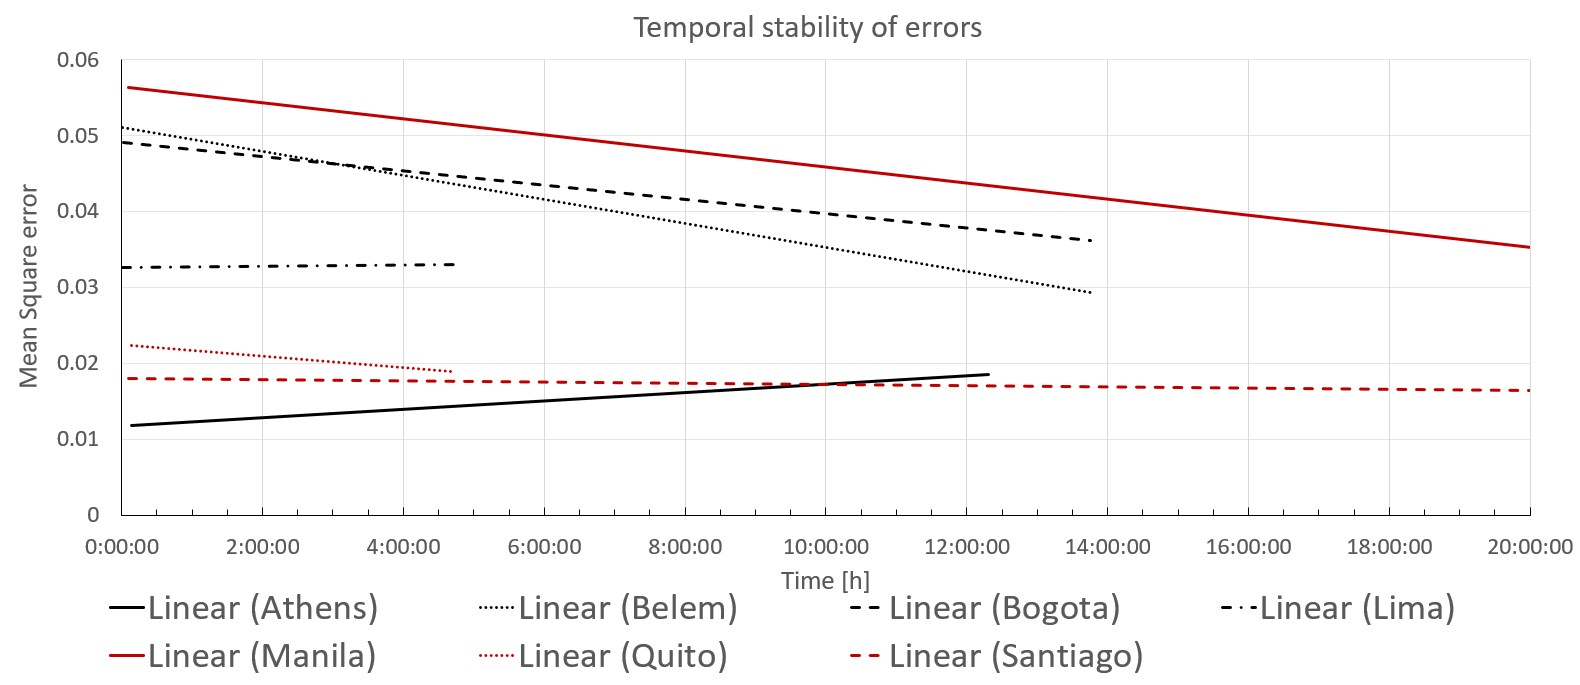
\includegraphics[width=\textwidth]{figures/chp_pdu/pdu_trend_iccs.jpg}
\caption{w funkcji czasu od kalibracji ustalającej błędy urządzenia~\cite{werner_experiment_driven_2022}}
\label{fig:pdu:trends:iccs}
\end{subfigure}

\smallskip
\begin{subfigure}{0.63\textwidth}
\centering
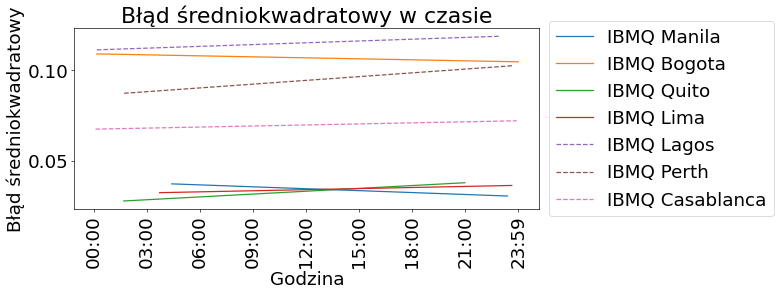
\includegraphics[width=\textwidth]{figures/chp_pdu/pdu_trend_msc.png}
\caption{w funkcji godziny doby~\cite{werner_magisterka_2022}}
\label{fig:pdu:trends:msc}
\end{subfigure}
\caption[Linie trendu błędu średniokwadratowego obwodu referencyjnego]{Linie trendu błędu średniokwadratowego wyników obwodu referencyjnego przed korektą, wyznaczone dla dwóch zbiorów danych: (a)~siedem urządzeń pięciokubitowych, (b)~urządzenia pięcio- i siedmiokubitowe.
Rysunki własne autora, przeniesione z~prac źródłowych bez zmian; na rysunku (a) oś pozioma to czas w~godzinach, a oś pionowa to błąd średniokwadratowy.}
\label{fig:pdu:trends}
\end{figure}

Linie trendu dają jedynie warunek konieczny stabilności: z nierówności trójkąta wynika, że zmiana błędu średniokwadratowego wyniku nieskorygowanego z wartości $\mathrm{MSE}_0$ do $\mathrm{MSE}_t$ ogranicza średni kwadrat dryfu tylko od dołu, $\langle\delta_t^2\rangle\ge\bigl(\sqrt{\mathrm{MSE}_t}-\sqrt{\mathrm{MSE}_0}\bigr)^2$; bezpośrednim oszacowaniem dryfu jest dopiero błąd po korekcie (podrozdział~\ref{subsec:pdu:results:one}).
% Usunięto przykład liczbowy (PHD-TS-91, ustalenia I5 i D15 recenzji): dla największej zmiany odczytanej z rysunku time stability.jpg (Belem, 0,0509 -> 0,0293 w 13,8 h) ograniczenie wynosi (sqrt(0.0509)-sqrt(0.0293))^2 = 0.0030, a dla urządzenia Manila (0.0563 -> 0.0353) 0.0024; wartości są orientacyjne, bo linie dopasowano do pomiarów z wielu dni, a ograniczenie dolne nie świadczy o stabilności.

\subsection{Korekta funkcji jednej zmiennej}\label{subsec:pdu:results:one}
\agentinfo{
Rysunek fig:pdu:example: cztery grafiki przeniesione z pracy magisterskiej (te same pliki są w katalogu artykułu): Quito, składnik o częstotliwości 2, zrzuty z 11.04.2022; Belem, MSE i odchylenie standardowe z 14.12.2021.
Wartości 0,0190, 0,0016, 0,1333 i 0,0401 podaje tylko artykuł (sekcja Results, słowa: in the cases shown there); po recenzji (ustalenie B2, PHD-TS-91) tekst przypisuje je artykułowi i podaje obok odczyt ze słupków rysunku (MSE 0,046 i 0,0005; odchylenie 0,21 i 0,02), który im nie odpowiada; krotność 12 i iloraz 8 procent usunięto.
Hipoteza recenzenta, niewpisana do tekstu: liczby artykułu są wartościami zbiorczymi dla urządzenia Quito (z r = 0,994 po korekcie wynika MSE około 0,0015 i odchylenie około 0,039).
Uwaga recenzenta do rozważenia przez autora, niewprowadzona: zbiorcze MSE po korekcie można oszacować pośrednio z wartości r po korekcie jako 0,125 razy (1/r^2 - 1), przy założeniu, że reszta nie jest skorelowana z wartością oczekiwaną (łącznie około 0,0033, od 0,0008 dla Limy do 0,0090 dla Belem); usunęłoby to lukę braku zbiorczych MSE.
Odczyt serii z urządzenia Belem (PHD-TS-91, skrypt recenzenta odczyt_serii.py): MSE przed korektą 0,029--0,062, po korekcie 0,006--0,015, iloraz 0,13--0,38 (mediana 0,25); oś czasu 33--162 minuty.
ROZBIEŻNOŚCI (DO DECYZJI AUTORA; w tekście zestawia je tabela tab:pdu:app:discrepancies w dodatku):
(1) dwa zbiory danych: artykuł ma 6006 próbek (tabela) albo 6005 (wykomentowany tekst: Belem 1248, Bogota 1857, Manila 1026, Quito 265), praca magisterska 10086; współczynniki Pearsona przed korektą różnią się (łącznie 0,876 wobec 0,761; Bogota 0,887 wobec 0,646);
(2) artykuł podaje przyrost dla Santiago 0.099, a plik pearson.png z katalogu artykułu 0.0099 (zgodne z wartościami 0.9785 i 0.99);
(3) praca magisterska podaje w tekście, że najmniejszy przyrost (0.0895) dotyczy urządzenia Manila, a z jej tabeli wynika 0.121 dla Manila i najmniejszy przyrost dla Athens (0.003), potem Quito (0.081);
(4) podpis rysunku z MSE i odchyleniem standardowym w artykule mówi o urządzeniu Lima i szeregu dwuskładnikowym, a włączone pliki pochodzą z urządzenia Belem (tak opisuje je praca magisterska);
(5) część rysunków przykładowych z czerwca 2022 r. ma oś argumentów opisaną od -2 pi do 3/2 pi (podwojone etykiety); tych rysunków nie przeniesiono.
Przedziały ufności w tabeli tab:pdu:corr obliczono w rozprawie przekształceniem Fishera z wartości r i N podanych w pracy magisterskiej.
Wykres fig:pdu:pearson (wartości r z tabel tab:pdu:corr i tab:pdu:app:iccs) przeniesiono w zadaniu PHD-TS-97 do dodatku, sekcja app:results:pdu2.
}

\begin{figure}[tb]
\centering
\begin{tabular}{@{}cc@{}}
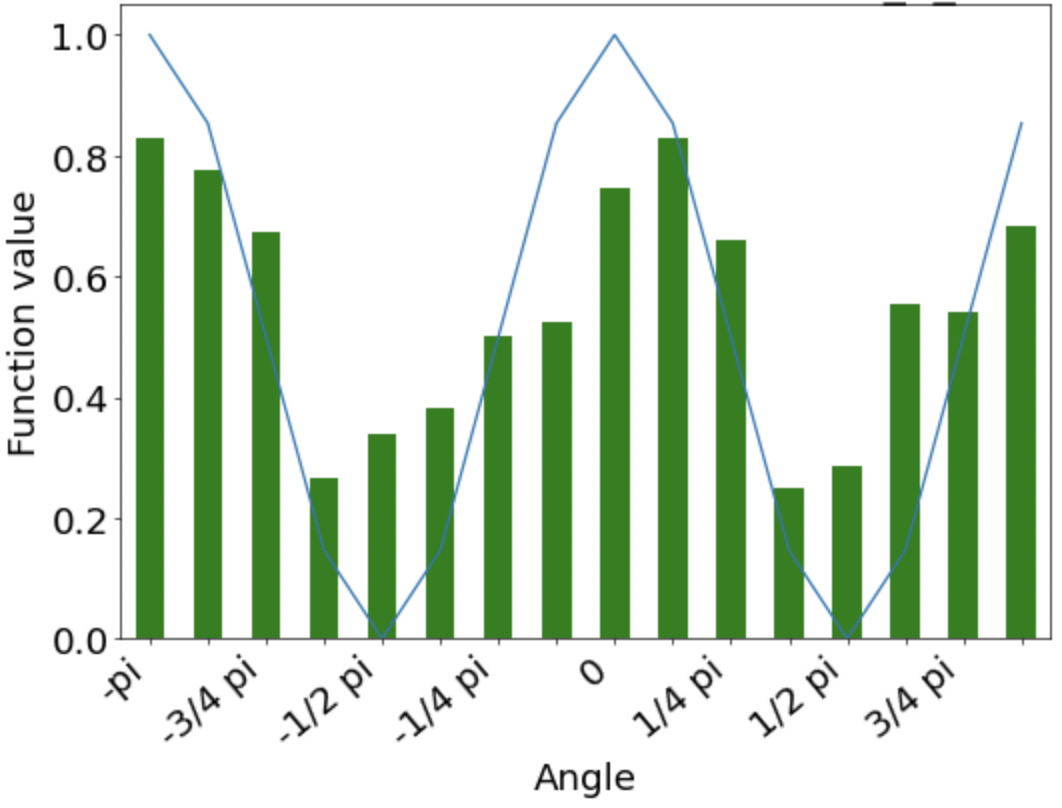
\includegraphics[width=0.30\textwidth]{figures/chp_pdu/pdu_quito_cos2x_before.png} &
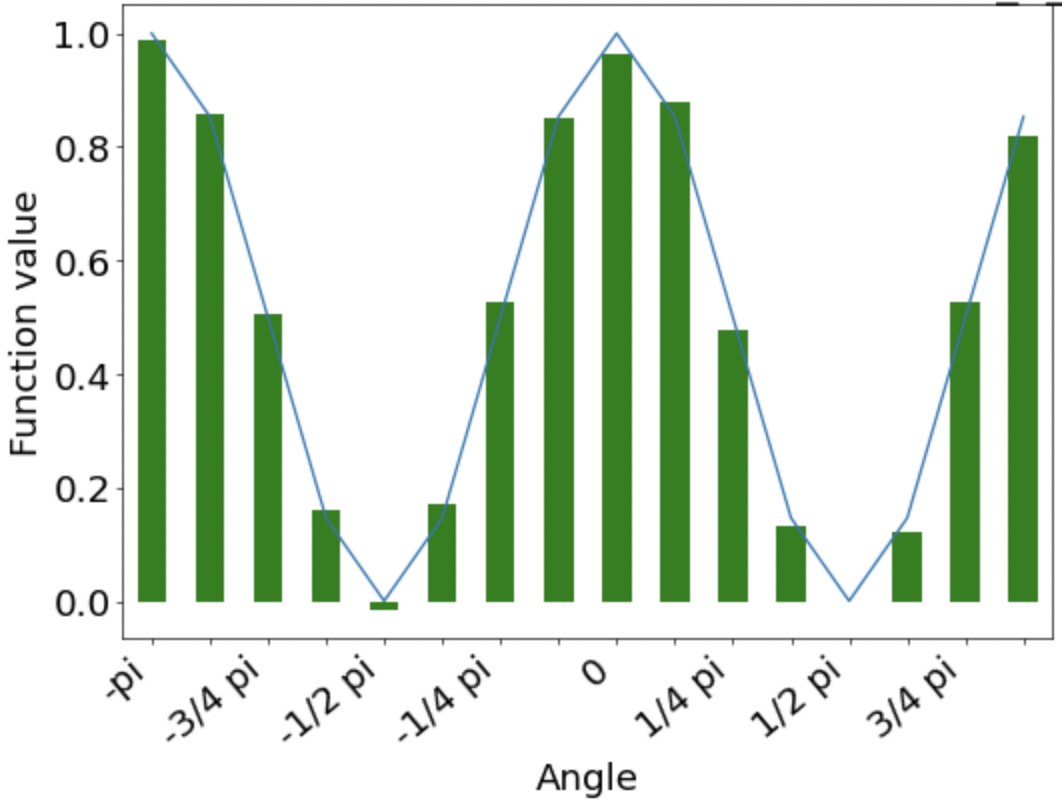
\includegraphics[width=0.30\textwidth]{figures/chp_pdu/pdu_quito_cos2x_after.png} \\
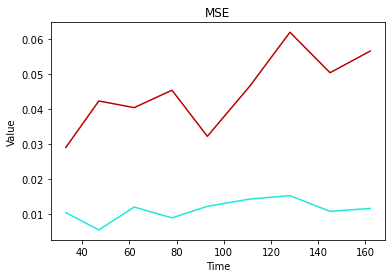
\includegraphics[width=0.30\textwidth]{figures/chp_pdu/pdu_belem_mse.png} &
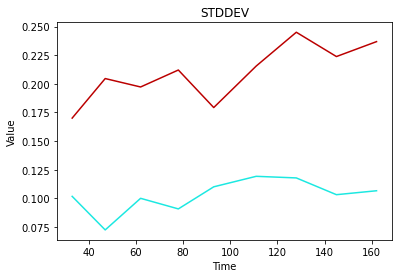
\includegraphics[width=0.30\textwidth]{figures/chp_pdu/pdu_belem_stddev.png}
\end{tabular}
\caption[Przykład korekty funkcją PDU na urządzeniach Quito i Belem]{Górny wiersz: wartości składnika $\coscomp_{2,0}$ uzyskane na urządzeniu Quito (słupki) na tle wartości oczekiwanych (linia), przed korektą (po lewej) i po korekcie (po prawej).
Dolny wiersz: błąd średniokwadratowy (po lewej) i odchylenie standardowe błędu (po prawej) kolejnych serii na urządzeniu Belem w~funkcji czasu od kalibracji funkcji PDU w~minutach; linia czerwona oznacza wynik przed korektą, linia turkusowa po korekcie.
Rysunki własne autora, przeniesione z~prac~\cite{werner_experiment_driven_2022,werner_magisterka_2022}.}
\label{fig:pdu:example}
\end{figure}

Działanie korekty na pojedynczym wyniku pokazuje górny wiersz rysunku~\ref{fig:pdu:example}: wartości składnika $\coscomp_{2,0}$ uzyskane na urządzeniu Quito 20~godzin po kalibracji urządzenia~\cite{werner_magisterka_2022}; czasu od kalibracji funkcji PDU źródła nie podają.
Praca~\cite{werner_experiment_driven_2022} podaje przy tym rysunku spadek błędu średniokwadratowego z $0{,}0190$ do $0{,}0016$ i odchylenia standardowego błędu z $0{,}1333$ do $0{,}0401$, ale odczyt wysokości słupków (dokładność około $0{,}002$) daje dla pokazanej serii MSE około $0{,}046$ przed korektą i $0{,}0005$ po niej; przy obu parach liczb błąd średniokwadratowy maleje ponad dziesięciokrotnie.
% ŹRÓDŁO: ICCS main.tex, sekcja Results, akapit ,,Significance of the PDU method'' (in the cases shown there); 20 godzin: magisterka 03.tex, opis rysunku fig:corrections_q.
% ŹRÓDŁO: odczyt z plików rozprawa/figures/chp_pdu/pdu_quito_cos2x_before.png i pdu_quito_cos2x_after.png skryptem eksperymenty/recenzje/_robocze/PHD-TS-62/odczyt_rysunkow.py (powtórzony w PHD-TS-91, plik powt_odczyt_rysunkow.txt): MSE 0,0459 i 0,0005; odchylenie standardowe błędu 0,2084 i 0,0204; rozdzielczość 0,0017--0,0018 na piksel; niezależny odczyt wzrokowy w PHD-TS-91 daje MSE przed korektą 0,046.
\agenttask{
Pytanie do autora (recenzja rozdziału 4, ustalenie B2): do której serii albo do jakiego zbioru odnoszą się wartości 0,0190, 0,0016, 0,1333 i 0,0401 z artykułu ICCS (pojedyncza seria z rysunku czy wartości zbiorcze dla urządzenia Quito) oraz ile czasu upłynęło między kalibracją funkcji PDU a serią pokazaną na rysunku?
Słupki na rysunku dają MSE około 0,046 przed korektą i 0,0005 po korekcie, więc liczby artykułu nie opisują pokazanej serii.
}%
Dolny wiersz przedstawia MSE i $\sigma_e$ dziewięciu kolejnych serii na urządzeniu Belem, od 33 do 162~minut po kalibracji funkcji PDU: według odczytu z rysunku błąd średniokwadratowy po korekcie stanowił od $13\%$ do $38\%$ błędu przed korektą.
% ŹRÓDŁO: odczyt z pliku rozprawa/figures/chp_pdu/pdu_belem_mse.png skryptem eksperymenty/recenzje/_robocze/PHD-TS-62/odczyt_serii.py (powtórzony w PHD-TS-91, plik powt_odczyt_serii.txt) w dziewięciu wierzchołkach linii (33, 47, 62, 78, 93, 111, 128, 145 i 162 min): przed korektą 0,029--0,062, po korekcie 0,0057--0,0154 (0,006--0,012 w pierwszych pięciu seriach, 0,011--0,015 w czterech ostatnich); ilorazy 0,13--0,38, mediana 0,25.
Ponieważ węzły kalibracji i węzły korygowanych wyników pokrywają się, wynik skorygowany jest tu sumą wartości oczekiwanej i różnicy dwóch pomiarów, korygowanego i kalibracyjnego.
Miary po korekcie oceniają zatem powtarzalność błędu między tymi pomiarami, a zgodnie ze wzorem~\eqref{eq:pdu:residual} błąd średniokwadratowy po korekcie jest bezpośrednim oszacowaniem średniego kwadratu dryfu.
Już w pierwszej serii, pół godziny po kalibracji, przekracza on granicę próbkowania $2/(4\nshots)\approx 6\cdot10^{-5}$ o dwa rzędy wielkości, więc dryf zawiera składową zmienną między kolejnymi seriami, a warunek~\eqref{eq:pdu:stability} jest spełniony tylko w słabym sensie kilkakrotnego zmniejszenia błędu.
% ŹRÓDŁO: obliczenie własne: 2/(4*8192) = 6,1e-5; MSE po korekcie w pierwszej serii około 0,010 (odczyt jak wyżej).

\begin{table}[tb]
\centering
\caption[Współczynniki korelacji wyników z wartościami oczekiwanymi przed korektą i po korekcie funkcją PDU]{Współczynniki korelacji wyników z wartościami oczekiwanymi przed korektą i po korekcie funkcją PDU: $r$ Pearsona z $95$-procentowym przedziałem ufności, $\tau$ Kendalla i $r_{\mathrm{S}}$ Spearmana; $N$ oznacza liczbę próbek.
Współczynniki i liczności według~\cite{werner_magisterka_2022}, przedziały ufności obliczone w rozprawie.}
\label{tab:pdu:corr}
\footnotesize
\begin{tabular}{@{}lrcccccc@{}}
\toprule
 & & \multicolumn{2}{c}{$r$ [95\% PU]} & \multicolumn{2}{c}{$\tau$} & \multicolumn{2}{c}{$r_{\mathrm{S}}$} \\
\cmidrule(lr){3-4}\cmidrule(lr){5-6}\cmidrule(l){7-8}
\textbf{Urządzenie} & $N$ & przed & po & przed & po & przed & po \\
\midrule
\multicolumn{8}{@{}l}{\emph{Funkcje jednej zmiennej (E3), urządzenia pięciokubitowe}} \\
Athens & 100 & 0,978 [0,967; 0,985] & 0,981 [0,972; 0,987] & 0,886 & 0,913 & 0,973 & 0,982 \\
Belem & 1248 & 0,836 [0,818; 0,852] & 0,966 [0,962; 0,970] & 0,653 & 0,843 & 0,828 & 0,956 \\
Bogota & 3760 & 0,646 [0,627; 0,664] & 0,978 [0,977; 0,979] & 0,516 & 0,866 & 0,649 & 0,968 \\
Lima & 1470 & 0,892 [0,881; 0,902] & 0,997 [0,997; 0,997] & 0,735 & 0,873 & 0,892 & 0,968 \\
Manila & 1667 & 0,855 [0,842; 0,867] & 0,976 [0,974; 0,978] & 0,693 & 0,874 & 0,852 & 0,969 \\
Quito & 1162 & 0,913 [0,903; 0,922] & 0,994 [0,993; 0,995] & 0,737 & 0,915 & 0,895 & 0,986 \\
Santiago & 679 & 0,875 [0,856; 0,892] & 0,990 [0,988; 0,991] & 0,737 & 0,901 & 0,866 & 0,982 \\
łącznie & 10\,086 & 0,761 [0,753; 0,769] & 0,987 [0,986; 0,987] & 0,580 & 0,900 & 0,741 & 0,979 \\
\midrule
\multicolumn{8}{@{}l}{\emph{Funkcja dwóch zmiennych (E5), urządzenia siedmiokubitowe}} \\
Casablanca & 5056 & 0,691 [0,676; 0,705] & 0,522 [0,502; 0,542] & 0,471 & 0,340 & 0,649 & 0,469 \\
Jakarta & 6208 & 0,506 [0,487; 0,524] & 0,363 [0,341; 0,384] & 0,384 & 0,328 & 0,532 & 0,457 \\
Lagos & 6272 & 0,378 [0,357; 0,399] & 0,355 [0,333; 0,376] & 0,239 & 0,236 & 0,343 & 0,331 \\
Perth & 4224 & 0,525 [0,503; 0,547] & 0,491 [0,468; 0,514] & 0,335 & 0,327 & 0,488 & 0,468 \\
łącznie & 21\,760 & 0,507 [0,497; 0,517] & 0,418 [0,407; 0,429] & 0,344 & 0,302 & 0,488 & 0,423 \\
\bottomrule
\end{tabular}
\end{table}
% ŹRÓDŁO tabeli: artykuły/magisterka_werner_final/chapters/03.tex, tabele tab:pearson_coefficients, tab:other_corrs_tau, tab:other_corrs_rho (E3) oraz tab:pearson_coefficients_seven, tab:other_corrs_seven (E5) i zdania z wartościami łącznymi; przedziały ufności: tanh(artanh(r) +/- 1,96/sqrt(N-3)).

W skali całego zbioru danych współczynniki korelacji wyników z wartościami oczekiwanymi wzrosły po korekcie na każdym urządzeniu (tabela~\ref{tab:pdu:corr}; rysunek~\ref{fig:pdu:pearson} w dodatku).
W zbiorze z pracy magisterskiej, liczącym $10\,086$ próbek, współczynnik Pearsona wzrósł z $0{,}761$ do $0{,}987$~\cite{werner_magisterka_2022}, a w mniejszym zbiorze opisanym w artykule ($6006$ próbek) z $0{,}876$ do $0{,}971$~\cite{werner_experiment_driven_2022}.
% ŹRÓDŁO: magisterka 03.tex, tabela tab:pearson_coefficients i zdanie pod nią; ICCS main.tex, sekcja Results (0.876, 0.9707) i tabela tab:coefficients (liczności; suma 6006 to obliczenie własne, w tekście artykułu nie pada).
Oba zbiory różnią się licznością i, poza urządzeniami Athens i Belem, wartościami współczynników przed korektą, zgodnie natomiast dają po korekcie wartości od $0{,}96$ do $1{,}00$.
Przedziały ufności współczynnika $r$ przed korektą i po korekcie są rozłączne dla wszystkich urządzeń z wyjątkiem Athens, także przy liczbie jednostek równej liczbie serii; dla urządzenia Athens zebrano tylko $100$ próbek, a korelacja już przed korektą wynosiła $0{,}978$, więc poprawy nie można uznać za wykazaną~\cite{werner_magisterka_2022}.
% ŹRÓDŁO: obliczenie własne z wartości r i N z tabeli tab:pdu:corr: tanh(artanh(r) +/- 1,96/sqrt(n-3)) dla n = N oraz n = N/16 (część całkowita); skrypt eksperymenty/recenzje/_robocze/PHD-TS-62/analiza_wrazliwosci.py, wynik powtórzony w PHD-TS-91 (plik powt_analiza_wrazliwosci.txt).
P-wartości oraz wyniki dla zbioru z artykułu zawiera dodatek (strona~\pageref{tab:pdu:app:pvalues}).
Według pracy~\cite{werner_magisterka_2022} funkcja PDU zmniejszała błąd nawet wiele godzin po kalibracji, do najbliższej kalibracji ustalającej nowe błędy urządzenia; źródło nie podaje przy tym liczb, a przykłady z osią czasu obejmują niespełna trzy godziny.
% ŹRÓDŁO: magisterka 03.tex, sekcja ,,Korekcja funkcji jednej zmiennej'', podsekcja ,,Wyniki eksperymentu'' (funkcja PDU skutecznie redukuje błąd nawet wiele godzin po kalibracji, dopóki nie nastąpiła kalibracja ustalająca nowe błędy); osie czasu rysunków fig:pdu:example (33--162 min) i fig:pdu:two-comp (18--94 min), odczyt skryptem odczyt_serii.py.
Dla badanych urządzeń pięciokubitowych odpowiedź na pytanie PB1 jest zatem twierdząca tylko w postaci słabszej, omówionej w podrozdziale~\ref{sec:pdu:discussion}.

\subsection{Korekta funkcji dwóch zmiennych i szeregów wieloskładnikowych}\label{subsec:pdu:results:two}
\agentinfo{
Rysunek fig:pdu:two-comp (od zadania PHD-TS-97 w dodatku, sekcja app:results:pdu2, razem z komentarzem źródłowym do dat w podpisie): trzy grafiki przeniesione z pracy magisterskiej (katalog wiele_komp; daty w nazwach plików 19.06.2022 i 19.01.2022); poziomy MSE (0,06--0,09 oraz poniżej 0,005) odczytano z osi wykresu, źródła nie podają dla tego eksperymentu statystyk zbiorczych ani sposobu kalibracji.
Wyniki eksperymentu dwóch zmiennych pochodzą wyłącznie z pracy magisterskiej (tabele tab:pearson_coefficients_seven i tab:other_corrs_seven); artykuł ich nie zawiera.
Rysunków z katalogu dwie_zmienne nie przeniesiono, bo praca magisterska ich nie opisuje i nie da się ustalić znaczenia serii.
Interpretacje dodane w rozprawie, DO AKCEPTACJI AUTORA: podwójne liczenie wspólnej części błędu przy sumowaniu poprawek oraz (po recenzji, ustalenie I7) uwaga, że sumowanie poprawek nie jest zastosowaniem definicji def:pdu:correction i że w modelu eq:tb:noise:fringe suma poprawek dla x i y nie jest poprawką dla x+y; praca magisterska mówi o pominiętym oddziaływaniu rejestrów i o możliwym współczynniku wagowym.
Recenzent policzył ilustrację liczbową tej uwagi (dla widoczności 0,7 i zerowego przesunięcia fazy korelacja spada po dodaniu sumy poprawek z 1,00 do 0,86); zgodnie z jego zaleceniem nie wprowadzono jej do tekstu bez decyzji autora.
Po recenzji (ustalenia I1, I2 i I6, PHD-TS-91): wniosek dla PB2 brzmi, że korekta poprawia wyniki obwodów, na których ją wyznaczono, a przenoszenia z funkcji referencyjnej na inne funkcje nie da się na podstawie źródeł potwierdzić; eksperyment E5 nazwano sprawdzeniem addytywności poprawek, a nie założenia Z8; dla E5 odporny jest wniosek o braku poprawy, nie o pogorszeniu (przedziały liczone dla serii zachodzą na siebie).
Odczyt słupków z rysunku fig:pdu:two-comp: przed korektą MSE 0,087 i korelacja z wartościami oczekiwanymi -0,53, po korekcie 0,0037 i +0,97.
Nazwa pliku z przebiegiem MSE na tym rysunku kończy się na MSE_cos_phi i ma datę 19.01.2022, a słupki pochodzą z 19.06.2022; praca magisterska opisuje przebieg jako wynik dla operatora wieloskładnikowego (pytanie do autora w zadaniu na końcu sekcji).
Zdanie proponujące powtórzenie eksperymentu w dwóch wariantach usunięto z tekstu (zasada: rozdział nie proponuje nowych eksperymentów); wcześniejsza propozycja z tego konspektu (E3 w dwóch wariantach kalibracji i E5 z pełną kalibracją na 64 obwodach, na symulatorze) pozostaje do decyzji autora i jest odłożona zgodnie z CLAUDE.md.
}

Dla szeregu dwuskładnikowego $\tfrac{1}{2}(\coscomp_{1,0}+\coscomp_{2,0})$, badanego na urządzeniu Lima (eksperyment E4), błąd średniokwadratowy kolejnych serii maleje po korekcie z poziomu $0{,}06$--$0{,}09$ do wartości poniżej $0{,}005$ (rysunek~\ref{fig:pdu:two-comp} w dodatku).
% ŹRÓDŁO: odczyt z rysunków wiele_komp/result_2_..., correctedResult_2_... i 01_19_2022_02_27_24_ibmq_lima_MSE_cos_phi.png (magisterka).
W pokazanej serii wynik nieskorygowany nie odtwarza jednak funkcji (odczyt ze słupków: korelacja z wartościami oczekiwanymi około $-0{,}5$ przed korektą i $0{,}97$ po korekcie), więc kształt widoczny po korekcie wnosi poprawka, a nie pomiar.
% ŹRÓDŁO: odczyt z plików rozprawa/figures/chp_pdu/pdu_lima_two_comp_before.png i pdu_lima_two_comp_after.png skryptem eksperymenty/recenzje/_robocze/PHD-TS-62/odczyt_rysunkow.py (powtórzony w PHD-TS-91, plik powt_odczyt_rysunkow.txt): r = -0,525 i +0,972; MSE 0,0866 i 0,0037 (osiem węzłów).
Sposobu kalibracji ani statystyk zbiorczych źródła nie podają, więc wynik ma charakter jakościowy i nie dowodzi przenoszenia korekty z funkcji referencyjnej.

Eksperyment E5 dał wynik negatywny.
Po korekcie sumą błędów obu rejestrów współczynniki korelacji zmalały na wszystkich czterech urządzeniach (tabela~\ref{tab:pdu:corr}): w zbiorze $21\,760$ próbek współczynnik Pearsona spadł z $0{,}507$ do $0{,}418$~\cite{werner_magisterka_2022}.
% ŹRÓDŁO: magisterka 03.tex, sekcja ,,Korekcja funkcji dwóch zmiennych'', podsekcja ,,Wyniki eksperymentu''.
Przedziały ufności liczone dla próbek są rozłączne dla zbioru łącznego oraz dla urządzeń Casablanca i Jakarta, a liczone dla serii zachodzą na siebie w każdym przypadku, więc odporny jest wniosek o braku poprawy, a nie o pogorszeniu.
% ŹRÓDŁO: obliczenie własne z wartości r i N z tabeli tab:pdu:corr dla n = N/64: łącznie n = 340, r = 0,507: [0,423; 0,582]; r = 0,418: [0,326; 0,502]; Casablanca (n = 79): [0,555; 0,791] i [0,340; 0,666]; Jakarta (n = 97): [0,341; 0,641] i [0,176; 0,524]; skrypt eksperymenty/recenzje/_robocze/PHD-TS-62/analiza_wrazliwosci.py, wynik powtórzony w PHD-TS-91.
Za prawdopodobną przyczynę uznano sposób kalibracji: błędy wyznaczone osobno dla każdego rejestru nie obejmowały oddziaływania rejestrów ani bramek drugiego rejestru~\cite{werner_magisterka_2022}.
Sumowanie poprawek nie jest ponadto zastosowaniem definicji~\ref{def:pdu:correction}, która wymagałaby funkcji PDU odczytanej dla fazy łącznej $x+y$: już w modelu~\eqref{eq:tb:noise:fringe} suma poprawek dla $x$ i $y$ nie jest na ogół poprawką dla $x+y$, a błąd odczytu, wspólny dla obu kalibracji, jest liczony dwukrotnie.
Żadnego z tych wyjaśnień nie sprawdzono: kalibracji na obwodach zawierających bramki obu rejestrów, w granicznym przypadku na wszystkich $64$ konfiguracjach, nie przeprowadzono.

Odpowiedź na pytanie PB2 jest zatem warunkowa, przy czym eksperyment E5 sprawdza inną hipotezę niż założenie~(\ref{itm:pdu:Z8}): addytywność poprawek rejestrów.
Korekta poprawia wyniki obwodów, na których ją wyznaczono, i nie przenosi się przez składanie poprawek wyznaczonych dla części układu; przenoszenia z funkcji referencyjnej na inne funkcje źródła nie pozwalają potwierdzić.
Praca~\cite{werner_experiment_driven_2022} opisuje wprawdzie korektę składnika $\coscomp_{2,0}$ funkcją wyznaczoną na funkcji referencyjnej, ale na rysunku~\ref{fig:pdu:example} poprawki w węzłach $x$ i $x+\pi$, o tej samej fazie $2x$ kubitu odczytu, różnią się nawet o $0{,}22$ (odczyt ze słupków).
% ŹRÓDŁO: odczyt jak w podrozdziale subsec:pdu:results:one (skrypt odczyt_rysunkow.py, plik powt_odczyt_rysunkow.txt): poprawka (wynik po korekcie minus przed korektą) w węzłach -3/8 pi i 5/8 pi: -0,209 i -0,431; w węzłach -1/8 pi i 7/8 pi: +0,321 i +0,136; błąd przed korektą w tych parach: +0,233 i +0,406 oraz -0,331 i -0,172; średnia kwadratowa różnic poprawek w ośmiu parach 0,109; niezależny odczyt wzrokowy w PHD-TS-91: -0,215 i -0,435 oraz +0,325 i +0,135.
Jeżeli oba panele pokazują tę samą serię, to przykład jest zgodny z tablicą wyznaczoną na obwodach korygowanego składnika, opisaną w pracy~\cite{werner_magisterka_2022}, i niezgodny z poprawką odczytywaną według samej fazy.
Wyznaczanie korekty raz dla rodziny obwodów jest więc potwierdzone dla obwodów jednej funkcji różniących się konfiguracją wejścia.
\agenttask{
Pytanie do autora (recenzja rozdziału 4, ustalenia I1 i I2): na jakich obwodach wyznaczano tablicę błędów użytą do korekty składnika o częstotliwości 2 (eksperyment E3) i szeregu dwuskładnikowego (eksperyment E4): na obwodach funkcji referencyjnej cos x, z odczytem poprawki dla fazy 2x, czy na tych samych obwodach, które potem korygowano?
Odczyt rysunku fig:pdu:example wskazuje drugi wariant (poprawki w węzłach o tej samej fazie różnią się nawet o 0,22), ale to jeden przykład i odczyt z rysunku rastrowego; po odpowiedzi doprecyzować wniosek dla PB2, zakres pierwszego wyróżnika metody w sekcjach 4.8 i 4.9 oraz brzmienie założenia Z8.
Dodatkowa obserwacja do tego samego pytania: nazwa pliku z przebiegiem MSE na rysunku fig:pdu:two-comp kończy się na MSE_cos_phi i ma datę 19.01.2022, a słupki pochodzą z 19.06.2022; czy ten przebieg dotyczy szeregu dwuskładnikowego?
}

\section{Dyskusja}\label{sec:pdu:discussion}
\agentinfo{
Napisane w zadaniu PHD-TS-57 (2026-11-27) z wyników sekcji 4.7 oraz z sekcji 3.3 i 3.5 i podrozdziału 2.3; bez nowych liczb i bez nowych pozycji bibliograficznych.
Decyzje autora z 2026-11-27: PDU jest metodą rozwijaną w ramach tego doktoratu i ważnym wkładem rozprawy; jej wyróżnikami względem metod pokrewnych są korekta indeksowana znanym argumentem, wyznaczana raz dla rodziny obwodów, oraz zbadanie stabilności błędu między kalibracjami urządzenia; metody pokrewne trzeba przywoływać (sekcja 3.3) i nie wolno pisać, że ich nie ma ani że PDU jest pierwsza.
Pytania rozdziału opisano słownie, bez numerów i bez brzmienia tezy (numeracja niezatwierdzona, zadanie pod akapitem).
Zgodnie z decyzją autora tekst nie proponuje nowych eksperymentów ani kierunków badań; mówi tylko, czego dane nie rozstrzygają.
Oceny własne, a nie twierdzenia cytowanych prac (DO AKCEPTACJI AUTORA): odczytanie wyników sekcji 4.7 jako potwierdzenia słabszej postaci założenia Z4; uwaga, że linia trendu może nie wykryć zmian skokowych; uwaga, że deklarowana kalibracja urządzenia wyznacza najwyżej górną granicę ważności funkcji PDU; zdanie o ponownym pomiarze węzłów jako sposobie rozpoznania nieaktualnej funkcji PDU (pomysł z konspektu sekcji 4.5, w eksperymentach niestosowany; to uwaga o regule ponownej kalibracji, nie propozycja badań).
Obserwacje o częstości kalibracji procesorów IBM pochodzą z sekcji 3.5: wilson_just-in-time_2020 dotyczy innych urządzeń i lat 2019--2020, a etxezarreta_multiqubit_2023 (dodatek C) tych samych procesorów pięciokubitowych (santiago i bogota kilka kalibracji na dobę; quito, belem i lima około jednej); roku tych pomiarów praca nie podaje (według notatki do sekcji 3.5 daty kwietniowe, preprint z lipca 2022), więc nie można wykluczyć, że pokrywają się z okresem eksperymentów PDU; dlatego tekst nie twierdzi, że pochodzą z innych dat.
Hipotezy o związku rozrzutu na urządzeniu Santiago z częstszymi kalibracjami nie wpisano (zadanie w sekcji 3.5).
Dopisane w zadaniu PHD-TS-94 (2026-11-27, po decyzji autora, że dawny rozdział 9 o strukturze szumu nie jest osobnym rozdziałem): trzy zdania na końcu akapitu o założeniu Z4, odnoszące się do pracy raubitzek_quantum_noise omawianej w sekcji 3.5 (akapit par:lr:noise:generators); praca jest pracą powiązaną z udziałem autora, a nie wkładem rozprawy.
Oceny własne w tych zdaniach (DO AKCEPTACJI AUTORA): warunek stabilności zaburzeń w schemacie z tej pracy jest odpowiednikiem założenia Z4; praca nie rozstrzyga o stałości błędu między kalibracjami; opis na poziomie generatorów jest uzupełnieniem, a nie uzasadnieniem metody PDU.
Zdania nie korzystają z elementów macierzy, których dotyczy ustalenie B1 recenzji dawnego rozdziału 9 \agentref{eksperymenty/recenzje/rozdzial-9.md}.
Zdanie, że rozdział opiera się na tekście, tabelach i rysunkach prac źródłowych, a nie na danych pierwotnych, zmienić, gdy autor dostarczy oryginalne dane eksperymentów PDU.
Pominięto dla objętości: osobne zdanie o mitygacji błędu odczytu (jest w podrozdziale 2.3 i w tabeli tab:lr:qem:calibrated); użyteczność metody poza erą NISQ (wstęp artykułu ICCS nazywa ją problematyczną); obserwację z wniosków artykułu ICCS, że urządzenia o bardziej poziomej linii trendu nie miały większego przyrostu korelacji; to, że zbiór z artykułu nie jest podzbiorem zbioru z pracy magisterskiej (dla urządzenia Belem tabela artykułu podaje 1360 próbek, a praca magisterska 1248; por. tabele tab:pdu:corr i tab:pdu:app:iccs); rozbieżności szczegółów protokołu opisane w konspekcie sekcji 4.6; zastrzeżenie, że poprawy dla urządzenia Athens nie wykazano (jest w sekcji 4.7.3).
Po recenzji (PHD-TS-91) uzgodniono dyskusję z poprawionymi sekcjami 4.4--4.7: odpowiedź o stabilności jest twierdząca w postaci słabszej (linie trendu nie pozwalają stwierdzić ani narastania błędu, ani jego stałości; korekta wyznaczona raz zwiększała zgodność wyników w badanych seriach), odpowiedź o przenoszeniu mówi, że korekta poprawia wyniki obwodów, na których ją wyznaczono, a przenoszenia między funkcjami źródła nie pozwalają potwierdzić; przy pierwszym wyróżniku podano zakres potwierdzenia (obwody jednej funkcji różniące się konfiguracją wejścia); usunięto słowa o poprawie przez wiele godzin i o braku wyraźnego trendu; dodano zdanie o nieudokumentowanej kontroli układu kubitów i transpilacji; trzy zdania podzielono.
Skróty z zadań PHD-TS-91 i PHD-TS-97 (wykazy w plikach wskazanych w konspekcie rozdziału): w dyskusji nie powtarza się zdania o przedziałach ufności, wyliczenia rozbieżności źródeł, zdania o wycofanych urządzeniach, wniosku o składaniu poprawek z eksperymentu E5 ani odesłania do wykresu współczynników korelacji; trzy zdania o pracy o zaburzeniach generatorów ściśnięto bez zmiany treści.
Objętość (kompilacja bez notatek, 2026-11-28, po przywróceniu schematu blokowego): treść zajmuje 16 stron i 6 wierszy na siedemnastej, w spisie treści rozdział ma 18 stron (rozdziały zaczynają się na stronie nieparzystej).
Decyzja autora z 2026-11-28: zostawić 17 stron, nie skracać rozdziału o te 6 wierszy.
Każde dalsze dopisanie zdania albo przywrócenie rysunku z dodatku wydłuża siedemnastą stronę; przekroczenie jej wymaga cięcia o tej samej wielkości.
}

W kategoriach kryteriów K1--K6 (tabela~\ref{tab:tb03:cost}) PDU nie zużywa dodatkowych kubitów ani bramek, a płaci wykonaniami obwodów kalibracyjnych (K3), założeniem o powtarzalności błędu (K5) i wąskim zakresem stosowalności metody zorientowanej na problem (K6); korekcji nie zastępuje, bo usuwa jedynie powtarzalną część błędu wyniku.
Samo to położenie nie wyróżnia jednak PDU: korektę wyznaczaną na obwodach o znanym wyniku i stosowaną klasycznie do wyniku niezmienionego obwodu zadania opisywano od 2020~r.~\cite{jattana_general_2020,czarnik_error_2021,urbanek_mitigating_2021,lolur_reference-state_2023}, a PDU jest własną realizacją tej zasady (podrozdział~\ref{sec:lr:qem}, tabela~\ref{tab:lr:qem:calibrated}).
Od metod tych odróżniają ją dwie cechy.
Po pierwsze, korekta jest tablicą błędów indeksowaną znanym argumentem, a nie funkcją wartości zmierzonej, i wyznacza się ją raz dla rodziny obwodów w każdym okresie między kalibracjami urządzenia, a nie osobno dla każdego obwodu zadania; w danych tego rozdziału rodzinę tę tworzą obwody jednej funkcji różniące się konfiguracją wejścia.
Samo wyznaczanie korekty raz dla obwodów o stałej strukturze ma odpowiednik w preprincie z 2025~r.~\cite{shen_circuit_2025}, więc odrębne dla PDU pozostaje w tej cesze indeksowanie znanym argumentem (podrozdział~\ref{sec:lr:qem}).
Po drugie, zbadano stabilność błędu między kalibracjami urządzenia (eksperymenty E2 i E3), a w tekstach głównych tamtych prac takich badań nie znaleziono.
Skalą demonstracji PDU nie wykracza natomiast poza prace pokrewne, a ceną pierwszej cechy jest wymóg znajomości argumentu (założenie~\ref{itm:pdu:Z7}): gdy argument nie jest znany, cecha ta nie ma zastosowania.

Na pytanie o stabilność błędu (podrozdział~\ref{sec:pdu:scope}) wyniki dają w zakresie badanych urządzeń pięciokubitowych odpowiedź twierdzącą w postaci słabszej: linie trendu nie pozwalają stwierdzić ani narastania błędu, ani jego stałości (rysunek~\ref{fig:pdu:trends}), a korekta wyznaczona raz zwiększała w badanych seriach zgodność wyników z wartościami oczekiwanymi, w obu zbiorach danych (tabela~\ref{tab:pdu:corr}).
Warunek~\eqref{eq:pdu:stability} sprawdzono bezpośrednio tylko w pojedynczych przykładach, do niespełna trzech godzin od kalibracji funkcji PDU (rysunek~\ref{fig:pdu:example}): zbiorczych wartości błędu średniokwadratowego po korekcie źródła nie podają, a współczynnik korelacji ocenia zgodność kształtu, nie wartości; dla urządzeń siedmiokubitowych dostępne są wyłącznie linie trendu.
Odpowiedź na pytanie o przenoszenie korekty pozostaje warunkowa (podrozdział~\ref{subsec:pdu:results:two}): korekta poprawia wyniki obwodów, na których ją wyznaczono, a tego, czy przenosi się między funkcjami, czyli jak szeroką rodzinę obwodów obsługuje jedna kalibracja, źródła nie pozwalają potwierdzić.
\agenttask{
Po zatwierdzeniu przez autora tez i numeracji pytań badawczych (sekcja sec:introduction:theses) dopisać w tym akapicie i w podsumowaniu rozdziału numery pytań, na które rozdział odpowiada (roboczo PB1 i PB2, tak jak w sekcjach 4.1, 4.2, 4.6 i 4.7), oraz zdanie odnoszące wyniki do tezy o redukcji błędów opartej na pomiarze (roboczo T1); do tego czasu nie przytaczać brzmienia tezy.
Uwaga orkiestratora do rozważenia przez autora (to nie jest decyzja): tezę T1 w brzmieniu ogólnym warto zawęzić do zakresu zbadanego w tym rozdziale.
}

Przegląd literatury w podrozdziale~\ref{sec:lr:noise} nie potwierdza założenia~(\ref{itm:pdu:Z4}) w postaci mocnej, czyli stałości błędu do następnej kalibracji urządzenia; zgodny jest z postacią słabszą, w której korekta wyznaczona z pomiaru zachowuje ważność przez czas rzędu godzin.
Wnioski te są pośrednie, bo przytoczone prace mierzą niemal wyłącznie parametry składowe, a nie błąd wyniku obwodu (tabela~\ref{tab:lr:noise:time}).
Zmiany tych parametrów bywają skokowe~\cite{klimov_fluctuations_2018,burnett_decoherence_2019}, a linia trendu, dopasowana do pomiarów z wielu okresów kalibracji, opisuje średnią zależność błędu od czasu, więc zmian epizodycznych w pojedynczym okresie nie wykrywa.
Czas od kalibracji jest ponadto wielkością deklarowaną przez dostawcę, a według innych prac częstość kalibracji procesorów IBM, także użytych w tym rozdziale, nie była stała i różniła się między urządzeniami~\cite{wilson_just-in-time_2020,etxezarreta_multiqubit_2023}, więc nie można przyjąć, że kalibracja była zawsze jednym zdarzeniem na dobę.
Wyniki podrozdziału~\ref{sec:pdu:results} należy zatem czytać jako stwierdzenie, że w badanych seriach korekta pozostawała korzystna, a nie jako dowód stałości błędu w całym okresie między kalibracjami.
Reguła ponownej kalibracji (podrozdział~\ref{sec:pdu:procedure}) wyznacza tym samym najwyżej górną granicę ważności funkcji PDU: warunek sprawdzany w algorytmie~\ref{alg:pdu:correction} jest konieczny, lecz niewystarczający.
Nieaktualna funkcja PDU, niespełniająca warunku~\eqref{eq:pdu:criterion}, może błąd zwiększać, a rozpoznać to pozwala dopiero ponowny pomiar węzłów, którego w eksperymentach nie stosowano.
Odpowiednikiem założenia~(\ref{itm:pdu:Z4}) jest warunek stabilności zaburzeń w schemacie diagnostycznym pracy o zaburzeniach generatorów bramek~\cite{raubitzek_quantum_noise} (podrozdział~\ref{par:lr:noise:generators}).
Praca ta nie rozstrzyga o stałości błędu między kalibracjami: zaburzenia dopasowano w niej do średniej z przebiegów zbieranych przez kilka miesięcy, nie rozdzielając rozrzutu między przebiegami na próbkowanie, dryf i zmiany kalibracji.
% ŹRÓDŁO: raubitzek_quantum_noise, wersja opublikowana (eksperymenty/_build/PHD-TS-38/work/pub/published.txt), sekcja VI.B, zastrzeżenie (2) (warunek stabilności), sekcja IV (dopasowanie do średniej z przebiegów) i sekcja VII (ponad pół roku zbierania danych); daty przebiegów w repozytorium danych pracy: od 2025-07-03 do 2025-10-15 (komentarz źródłowy w akapicie par:lr:noise:generators sekcji 3.5).
Wobec metody PDU, która bramek nie modeluje (założenie~\ref{itm:pdu:Z2}), opis na poziomie generatorów jest zatem uzupełnieniem, a nie uzasadnieniem.

Wyniki dotyczą obwodów metody QCoSamp z jednym kubitem odczytu na urządzeniach pięcio- i siedmiokubitowych, a funkcja PDU jest związana z rodziną obwodów, urządzeniem, układem kubitów i sposobem transpilacji (założenia~\ref{itm:pdu:Z2} i~\ref{itm:pdu:Z5}), więc nie przenoszą się wprost na inne obwody ani na większe urządzenia; kontroli układu kubitów i transpilacji między kalibracją a seriami korygowanymi źródła nie dokumentują.
Rozdział opiera się na tekście, tabelach i rysunkach dwóch prac, nie na danych pierwotnych; część wartości odczytano z rysunków.
Rozbieżności między źródłami (tabela~\ref{tab:pdu:app:discrepancies}) nie da się wyjaśnić bez danych pierwotnych, dlatego wnioski oparto na tym, w czym oba źródła są zgodne.
W eksperymencie E3 miary po korekcie oceniają powtarzalność błędu w tych samych węzłach, a nie wyznaczanie nieznanej wartości; interpolacji między węzłami nie używano w żadnym eksperymencie.
Wyjaśnienie negatywnego wyniku eksperymentu E5 pozostaje hipotezą, a koszt pełnej kalibracji rośnie wykładniczo z łączną liczbą kubitów rejestrów argumentu (podrozdział~\ref{sec:pdu:procedure}), co ogranicza skalowalność korekty tablicowej.

We wszystkich eksperymentach tego rozdziału argument korekty był znany z konstrukcji obwodu (podrozdział~\ref{par:pdu:known-argument}), więc nie mówią one, jak metoda zachowuje się, gdy faza kubitu odczytu zależy od danych nieznanych w chwili korekty (rozdział~\ref{chapter:pdu_images}).
Przeniesienie samej zasady korekty kalibrowanej z pomiaru na uczone kodowanie obrazów i na klasyfikator badają rozdziały~\ref{chapter:learned_encoding} i~\ref{chapter:classification}; wyniki są tam warunkowe, a w części negatywne (podrozdziały~\ref{sec:le:summary} i~\ref{subsec:cls:results:pdu}).

\section{Podsumowanie}\label{sec:pdu:summary}
\agentinfo{
Napisane w zadaniu PHD-TS-57 (2026-11-27): zebranie ustaleń rozdziału bez nowych treści i bez liczb; oba wyróżniki metody w brzmieniu z decyzji autora z 2026-11-27 (por. sekcja 3.3).
Po recenzji (PHD-TS-91): dopisano zakres, w jakim dane potwierdzają pierwszy wyróżnik, zdanie o trendzie doprowadzono do poziomu danych, a dla funkcji dwóch zmiennych napisano, że korekta wyników nie poprawiła (zamiast: pogorszyła).
Przejście do rozdziału 5 nie przesądza skuteczności PDU dla obrazów (sprawa otwarta, CLAUDE.md).
Numery pytań badawczych i odniesienie do tezy dopisać po decyzji autora (zadanie w sekcji 4.8).
Przy skracaniu (PHD-TS-97) usunięto z podsumowania powtórzenie zdania o liniach trendu (jest w sekcjach 4.7.2 i 4.8; wniosek, że dane nie rozstrzygają stałości błędu, pozostał).
}

W rozdziale przedstawiono metodę PDU, rozwijaną w ramach tej rozprawy: jej definicje, osiem założeń, procedurę kalibracji i korekty wraz z kosztem oraz ilościowy zapis założenia stabilności.
Metoda jest własną realizacją zasady korekty wyniku kalibrowanej na obwodach o znanym wyniku, a jej wyróżnikami, na których opiera się wkład rozprawy, są korekta indeksowana znanym argumentem, wyznaczana raz dla rodziny obwodów, oraz zbadanie stabilności błędu między kalibracjami urządzenia; pierwszy dane potwierdzają dla obwodów jednej funkcji różniących się wejściem.
Na badanych urządzeniach pięciokubitowych korekta wyznaczona raz zwiększała w badanych seriach zgodność wyników funkcji jednej zmiennej z wartościami oczekiwanymi w obu zbiorach danych; dla funkcji dwóch zmiennych korekta złożona z poprawek obu rejestrów wyników nie poprawiła.
Dane nie rozstrzygają stałości błędu w całym okresie między kalibracjami ani przenoszenia korekty między funkcjami, a metoda wymaga argumentu znanego w chwili korekty.
Ten ostatni wymóg jest punktem wyjścia rozdziału~\ref{chapter:pdu_images}, który bada zastosowanie metody do kodowania i rekonstrukcji obrazów.

% !TeX root = ./../main.tex

\chapter{Redukcja błędów w kodowaniu i rekonstrukcji obrazów kwantowych}\label{chapter:pdu_images}

\agentinfo{
Rozdział przenosi metodę PDU na kwantowe przetwarzanie obrazów i bada utratę danych w metodach reprezentacji.
Źródła:
artykuł KES 2023 o utracie danych \agentref{bib:werner_data_loss_2023} \agentref{artykuły/PROCS_KES2023_LATEX_Template/k23-558.tex},
artykuł CoDIT 2025 o schemacie kodowanie--rekonstrukcja \agentref{bib:werner_error_reduction_2025} \agentref{artykuły/CoDIT_2025_final_paper/root.tex},
rysunki \agentref{artykuły/PROCS_KES2023_LATEX_Template/imgs} \agentref{artykuły/CoDIT_2025_final_paper/imgs}.
Katalogi Quantum_Errors_ICCS_Images i Artykuł_2025_PDU_conf zawierają wcześniejsze wersje artykułu CoDIT i służą tylko pomocniczo.
Definicje FRQI, NEQR, LPIQE i miar jakości znajdują się w zapleczu teoretycznym \agentref{chapters/theoretical_background_05_QIMG.tex}; tutaj tylko odwołania.
}

\section{Cel i zakres rozdziału}\label{sec:pdui:scope}
\agentinfo{
Pytanie badawcze rozdziału: PB3.
Odniesienie do tez T1 i T2.
}

\section{Schemat kodowania i rekonstrukcji obrazu}\label{sec:pdui:scheme}
\agentinfo{
Potok: obraz, wektoryzacja, operator LPIQE, operator rekonstrukcji, pomiar, odtworzenie intensywności, korekta PDU.
Hybrydowy charakter: obliczenia na komputerze kwantowym, redukcja błędu na komputerze klasycznym.
Dwa scenariusze użycia zakodowanego obrazu: przetwarzanie wewnątrz procesora kwantowego oraz przesłanie do innego układu (komunikacja kwantowa).
}

\section{Uogólnienie funkcji PDU na przetwarzanie obrazów}\label{sec:pdui:generalisation}
\agentinfo{
Uogólniona definicja PDU: funkcja określona na parach (stan bazowy, faza), wyznaczana eksperymentalnie.
Kalibracja dla układu kubitów użytego do kodowania obrazu, ziarnistość pomiarów kalibracyjnych.
Źródło: sekcja Error reduction artykułu CoDIT.
}

\section{Metodyka badań eksperymentalnych}\label{sec:pdui:methodology}
\agentinfo{
Dane: obrazy monochromatyczne 8x8 i 16x16, liczba obrazów, sposób generowania.
Środowisko: rzeczywiste urządzenia IBM Quantum (nazwy, daty) oraz symulatory; liczba powtórzeń.
Implementacje FRQI, NEQR i LPIQE użyte w porównaniu.
Miary: MSE, odchylenie standardowe błędu, korelacja Pearsona z p-wartością.
Źródła: sekcje Experimental protocol obu artykułów.
}

\section{Wyniki}\label{sec:pdui:results}

\subsection{Utrata danych w metodach reprezentacji na symulatorze}\label{subsec:pdui:results:sim}
\agentinfo{Źródło: artykuł KES, sekcja o obrazach 8x8 na symulatorze.}

\subsection{Utrata danych w metodach reprezentacji na rzeczywistych urządzeniach}\label{subsec:pdui:results:real}
\agentinfo{Źródło: artykuł KES, sekcja o obrazach 8x8 na rzeczywistych urządzeniach.}

\subsection{Redukcja błędów dla obrazów \texorpdfstring{$8\times8$}{8x8} na rzeczywistych urządzeniach}\label{subsec:pdui:results:pdu8}
\agentinfo{Źródła: artykuł KES (sekcja o redukcji błędów z LPIQE) i artykuł CoDIT (sekcja real-comp).}

\subsection{Redukcja błędów dla obrazów \texorpdfstring{$16\times16$}{16x16} na symulatorze}\label{subsec:pdui:results:pdu16}
\agentinfo{Źródło: artykuł CoDIT, sekcja simulator.}

\section{Dyskusja}\label{sec:pdui:discussion}
\agentinfo{
Odpowiedź na PB3.
Weryfikacja tezy T2: porównanie MSE po PDU z błędem standardowych metod kompresji stratnej; artykuły nie zawierają takiego porównania wprost, więc może być potrzebny dodatkowy, prosty eksperyment klasyczny (do decyzji autora).
Kompromis między liczbą kubitów a jakością rekonstrukcji w FRQI, NEQR i LPIQE.
Znaczenie dla platform fotonicznych i komunikacji kwantowej.
Ograniczenia: małe rozmiary obrazów, operator definiowany macierzą i koszt jego transpilacji, eksperymenty wyłącznie na urządzeniach nadprzewodzących i symulatorach.
}

\section{Podsumowanie}\label{sec:pdui:summary}

% !TeX root = ./../main.tex

\chapter{Uczenie głębokie jako narzędzie redukcji błędów}\label{chapter:dl_error_reduction}

\agentinfo{
Rozdział opisuje użycie generatywnej sieci przeciwstawnej pix2pix do redukcji błędu w obrazach kodowanych metodą LPIQE, samodzielnie oraz w połączeniu z PDU.
Praca nie została opublikowana w czasopiśmie; istnieje jako preprint z 2023 r. (Preprints.org) i tak należy ją cytować.
Docelowa objętość rozdziału: około 10 stron.
Źródła:
manuskrypt w szablonie czasopisma Quantum (wersja po korekcie językowej, traktować jako nadrzędną) \agentref{bib:werner_deep_learning_manuscript} \agentref{artykuły/Quantum_journal_GAN__Copy_/article.tex},
ten sam manuskrypt w szablonie MDPI \agentref{artykuły/Energies_article/template.tex},
rysunki \agentref{artykuły/Quantum_journal_GAN__Copy_/imgs}.
Podstawy sieci GAN i pix2pix są w zapleczu teoretycznym \agentref{chapters/theoretical_background_06_ML.tex}.
}

\section{Cel i zakres rozdziału}\label{sec:dl:scope}
\agentinfo{
Pytanie badawcze rozdziału: PB4.
Odniesienie do roboczej tezy T3.
}

\section{Redukcja błędu jako translacja obraz--obraz}\label{sec:dl:concept}
\agentinfo{
Sformułowanie zadania: wejściem jest obraz zrekonstruowany z pomiarów (surowy albo po PDU), wyjściem obraz zbliżony do oryginału.
Uzasadnienie: zniekształcenie jest systematyczne i zależne od urządzenia, więc może być wyuczone.
Miejsce sieci w potoku: po rekonstrukcji i po PDU, w całości po stronie klasycznej.
}

\section{Architektura sieci}\label{sec:dl:architecture}
\agentinfo{
Generator U-Net (liczba parametrów, bloki kodujące i dekodujące, połączenia skrótowe), dyskryminator PatchGAN, funkcja straty z wagami 1 i 100, optymalizator Adam z parametrami.
Skalowanie obrazów do 256x256 i z powrotem; omówić konsekwencje.
Schematy architektury wykonać na nowo w TikZ zamiast przenosić rastrowe rysunki z manuskryptu.
}

\section{Protokół eksperymentalny}\label{sec:dl:protocol}
\agentinfo{
Cztery eksperymenty:
E1: obrazy 16x16 z symulatora, odniesieniem obrazy po PDU;
E2: obrazy 8x8 z rzeczywistego urządzenia, odniesieniem obrazy po PDU;
E3: obrazy 16x16 z symulatora po PDU, odniesieniem obrazy oryginalne;
E4: obrazy 8x8 z rzeczywistego urządzenia po PDU, odniesieniem obrazy oryginalne.
Zbiory: 631 obrazów (symulator) i 61 obrazów (urządzenie IBMQ Nairobi); liczba epok 250 i 1000.
Opisać podział na zbiór uczący i testowy oraz kroki odtworzenia eksperymentu.
W manuskrypcie tytuły podrozdziałów wyników i lista eksperymentów nie są w pełni spójne; uzgodnić numerację z danymi przed opisem.
}

\section{Wyniki}\label{sec:dl:results}

\subsection{Obrazy z symulatora}\label{subsec:dl:results:sim}
\agentinfo{Eksperymenty E1 i E3.}

\subsection{Obrazy z rzeczywistego urządzenia}\label{subsec:dl:results:real}
\agentinfo{
Eksperymenty E2 i E4.
Wynik kluczowy do zweryfikowania w danych: MSE rzędu 0,00014 i odchylenie standardowe błędu 0,00993 dla E4.
}

\subsection{Porównanie: wynik surowy, PDU, sieć, PDU z siecią}\label{subsec:dl:results:comparison}
\agentinfo{Tabela zbiorcza miar dla wszystkich wariantów.}

\section{Dyskusja}\label{sec:dl:discussion}
\agentinfo{
Odpowiedź na PB4.
Zagrożenia trafności, które trzeba omówić wprost:
bardzo mały zbiór z rzeczywistego urządzenia (61 obrazów) i ryzyko przeuczenia;
ryzyko, że sieć odtwarza rozkład danych uczących zamiast usuwać szum (obraz wiarygodny wizualnie, lecz niezgodny z pomiarem);
zależność wytrenowanej sieci od urządzenia i od kalibracji;
koszt treningu sieci o ponad 54 milionach parametrów dla obrazów 8x8 i 16x16;
skalowanie na większe obrazy.
Jeśli dane na to pozwalają, rozważyć eksperymenty uzupełniające: walidację krzyżową, test na obrazach spoza rozkładu, prostsze modele odniesienia (do decyzji autora).
}

\section{Podsumowanie}\label{sec:dl:summary}

% !TeX root = ./../main.tex

\chapter{Uczone kodowanie obrazów na rzeczywistym sprzęcie kwantowym}\label{chapter:learned_encoding}

\agentinfo{
Rozdział opisuje hybrydowy autoenkoder, w którym sieć klasyczna uczy się kodować obraz w płytki obwód kwantowy, oraz zachowanie tego kodowania na rzeczywistym urządzeniu.
Jest to kolejny etap linii badań z rozdziałów 5 i 6: kodowanie i rekonstrukcja obrazu pod szumem.
Docelowa objętość: około 12 stron.

Źródło: katalog /Users/krzysztofwerner/Downloads/Quantum/best_results_package (tylko do odczytu; nie czytać plików .env).
Manuskrypt roboczy article/main.tex jest współautorski i nieopublikowany; wkład autora rozprawy trzeba oddzielić od wkładu współautorów.
Liczby brać z plików wynikowych (article/data/eval_results.json, article/data/hw_results.json, output/hw_run1/analysis/report.md, hw_run2_finetune/baseline/summary.md), a nie z tekstu manuskryptu.
Zweryfikowany zestaw 363 liczb ze wskazaniem pliku i pola (zadanie PHD-TS-77): \agentref{eksperymenty/weryfikacja-liczb/rozdzial-7.md} \agentref{eksperymenty/weryfikacja-liczb/rozdzial-7.csv}.

Akcent rozdziału: charakterystyka szumu urządzenia, budżet błędu i redukcja błędów, a nie jakość samego kodowania.
Dwa punkty odniesienia, których nie wolno mylić (model 9x9, 10 niewidzianych obrazów, MAE): obraz średni zbioru uczącego 0,1329 oraz płaski obraz w średnim kolorze danego obrazu 0,0833.
Od obrazu średniego model jest lepszy: 0,0787 w symulatorze z szumem i 0,1009 na sprzęcie.
Od płaskiego obrazu własnego koloru jest w symulatorze lepszy tylko nieznacznie (różnica -0,0046, przedział ufności obejmuje zero, p = 0,34), a na sprzęcie gorszy na wszystkich 10 obrazach; należy to napisać wprost.
Płaski obraz własnego koloru odpowiada przekazaniu trzech liczb na obraz; opisać, co to porównanie mówi o informacji przenoszonej przez kodowanie.
Wyniki negatywne i nierozstrzygające (trening w szumie, dostrajanie na sprzęcie) są pełnoprawną treścią rozdziału.

Zagrożenia do opisania przy liczbach: duplikaty obrazów między zbiorem walidacyjnym a uczącym (4 z 14; rzetelna ocena na 10 niewidzianych obrazach), nakładanie się kafli o 50 pikseli (8 z 10 obrazów testowych przebiegu H2 nakłada się z kaflami uczącymi), wszystkie kafle z dwóch klatek, wybór punktu kontrolnego oraz dobór hiperparametrów i wariantu 16x16 na zbiorze, na którym raportowano wynik, model szumu dopasowany na obwodach testowych, bardzo mała próba, jedno urządzenie i jedno ziarno losowe.
Miarą główną w źródle jest MAE; korelacji Pearsona nie ma w plikach wynikowych, a MSE jest tylko dla przebiegu H2 i modelu 9x9.

Stan: sekcje 7.1--7.3 napisane w zadaniu PHD-TS-76 (2026-11-27); podrozdziały 7.4.1--7.4.3 z tabelami i rysunkami napisane w zadaniach PHD-TS-81 i PHD-TS-82 (2026-11-27); podrozdział 7.4.4 z rysunkiem fig:le:pdu:curves oraz sekcje 7.5 i 7.6 napisane w zadaniu PHD-TS-83 (2026-11-27); cały rozdział ma treść, czeka na przegląd autora i na odpowiedzi na pytania zapisane w zadaniach.
Poprawki po niezależnej recenzji (zadanie PHD-TS-85, plik \agentref{eksperymenty/recenzje/rozdzial-7.md}) wprowadzono w zadaniu PHD-TS-92 (2026-11-27); tabela statusów ustaleń: \agentref{eksperymenty/recenzje/rozdzial-7-poprawki.md}.
Na autora czekają: podział wkładu (zadanie w sekcji 7.1), pochodzenie kafli lotniczych i parametrów poziomu 4 (zadania w sekcji 7.3), galeria rekonstrukcji (zadanie w 7.4.2), tabela wariantów korekty w dodatku i skracanie rozdziału (zadanie w 7.4.4).
Objętość po poprawkach jest taka sama jak przed nimi (14,81 strony bez notatek: strony 75--89, ostatnia zapełniona w 0,81), bo dopisane zdania skompensowano skróceniem powtórzeń; do przywrócenia po decyzji o objętości nadają się: (a) w 7.2 pełniejsze porównanie z FRQI, NEQR i LPIQE (dokładne odtwarzanie bez szumu i przy nieskończonej liczbie pomiarów, zależność obwodu kodującego od obrazu, zajęcie 3W^2 stanów bazowych przez obraz barwny) i dwa zdania powtarzające podrozdział 2.6.4; (b) w 7.4.1 zdanie, że w zbiorze KITTI płaski obraz własnego koloru (0,2039) jest gorszy od obrazu średniego (0,1861), a A16K lepszy od obu (liczby są w tabeli tab:le:sim); (c) w 7.4.2 zdanie przejściowe do 7.4.4 o tym, że składnik depolaryzacyjny ma w przybliżeniu postać ze wzoru eq:le:noise, a jego odwrócenie wzmacnia szum próbkowania; (d) w 7.4.3 uwaga, że trening z szumem nie zapobiegł wzrostowi błędu o 28 procent; (e) w 7.4.4 szczegóły: 50 losowych podziałów, liczby TVD i wierności kontroli syntetycznej, skład kalibracji z tego samego dnia (wagi zmieniane między zadaniami), przedział ufności dla korekty addytywnej na obrazach KITTI, udział około trzech czwartych w mierze MAE; (f) w 7.5 akapit porównania z reprezentacjami zadanymi wzorem (teraz jedno zdanie z odesłaniem do 7.2) i zdanie, że pomiary nie wykluczają zmiany błędu obrazu o mniej niż około 0,003; (g) w 7.6 piąte zdanie podsumowania.
Ustalenia nazewnicze z sekcji 7.1--7.3, obowiązujące w wynikach:
(0) Oznaczenia konfiguracji zmieniono w zadaniu PHD-TS-92 z M8, M9, M16, M16K na A8, A9, A16, A16K, bo kolidowały z modelami klasyfikatora M1--M11 z rozdziału 8 (tabela tab:cls:models); stare oznaczenia występują jeszcze poza rozprawą w recenzji (eksperymenty/recenzje/rozdzial-7.md) i w jej plikach roboczych. Litery A w oznaczeniu konfiguracji nie mylić ze zbiorem A eksperymentu na symulatorze (punkt 2).
(1) Konfiguracje (tabele tab:le:configs i tab:le:data): A8 = RGB 8x8, 9 kubitów, 8 bloków, bez szumu w treningu (klucz c8 w eval_results.json, punkt kontrolny run_2026-08-12_21-21-32); A9 = RGB 9x9, 9 kubitów, 8 bloków, trening z szumem poziomu 4 (run_2026-10-13_09-57-33); A16 = RGB 16x16, 11 kubitów, 12 bloków (klucz c16_best); A16K = KITTI 16x16, 11 kubitów, 13 bloków (klucz c16_kitti2000).
(2) Zbiory oceny: K16 = 16 kafli części testowej eksportu (A8); K12 = 12 kafli walidacyjnych podziału losowego (A16); K10 = 10 kafli walidacyjnych bez kopii w części uczącej (A9), zarazem zbiór testowy przebiegu H2 i część testowa zbioru A w eksperymentach sekcji 7.4.4; dla KITTI 1500 obrazów testowych. Wartości na nominalnych 14 obrazach walidacyjnych A9 (np. MAE 0,0732) nie raportować jako wyniku.
(3) Symulatory: symulator bezszumowy; symulator poziomu 4 (odstrojenie 0,0012756 rad i depolaryzacja 0,0029837 na kubit po każdym bloku, bez tłumienia fazy i bez błędu odczytu); bliźniak (model warstwowy z samą depolaryzacją dopasowaną do zliczeń z urządzenia; wartość dopasowana jest wynikiem i należy do sekcji 7.4.2). Skończona liczba pomiarów: losowanie z rozkładu symulatora, średnia z 3 losowań (wyjątek w plikach H2: wiersz ,,poziom 4, 16 384 pomiary'' to jedno losowanie).
(4) Przebiegi: H1 (sierpień 2026, A8, 228 pomiarów rejestrów, 9 łańcuchów, obrazy KITTI spoza rozkładu; w podrozdziałach 7.4.1--7.4.3 tylko miary rozkładu, w 7.4.4 MAE obrazu wyłącznie do porównania wariantów korekty, z dolną granicą 0,154) i H2 (3 listopada 2026, A9, 5 łańcuchów, K10; zadanie bazowe, pięć zadań dostrajania, zadanie końcowe).
(5) Punkty odniesienia: obraz średni (średnia po obrazach części uczącej, osobno dla piksela i kanału) oraz płaski obraz własnego koloru (stała w każdym kanale równa średniej tego kanału w obrazie ocenianym; trzy liczby na obraz). Trzeciego wariantu z plików H2, płaskiego obrazu w średnim kolorze części uczącej (MAE 0,1333), nie używać. Dla KITTI obraz średni w eval_article.py policzono z innej losowej próby 2000 obrazów uczących niż użyta w treningu.
(6) Miary: MAE na wyjściu nieobciętym; PSNR i SSIM na wyjściu obciętym do przedziału od 0 do 1, liczone na obraz i uśredniane; SSIM z oknem Gaussa 5x5 o odchyleniu 1, stałe 0,01^2 i 0,03^2 (wartości z eval_results.json i hw_results.json, nie z summary.csv ani summary.md); MSE tylko dla A9 i H2 (summary.csv, wyjście nieobcięte); wierność Hellingera (makro hfid, etykieta eq:le:hellinger), TVD, odległość Hellingera, wierność znormalizowana; porównania sparowane: bootstrap 10 000 losowań i dokładny dwustronny test znaków.
(7) Notacja: kubity numerowane od 0 do n, kubit 0 to kubit pomocniczy a (litera q jest zajęta przez parametry kanałów); liczba bloków L; kąty bloku jako składowe wektora theta; wartość odczytana u_j przed splotem i intensywność odtworzona po splocie; współczynnik skali modelu kalibracyjnego c_kal (w plikach H1 nazywany lambda, ale lambda jest w pracy parametrem depolaryzacji); parametry modelu warstwowego jak w podrozdziale 2.2 (makra qdep, cohangle, qphase).
(8) Odchylenia standardowe w plikach: H1 z mianownikiem n, H2 z mianownikiem n-1.
(9) Odwołania przez ref z polskim rzeczownikiem, jak w pozostałych rozdziałach: pakiet cleveref nie ma polskich nazw i w pracy nie jest używany.
(10) Etykiety wyników z podrozdziałów 7.4.1--7.4.3, do odwołań w 7.4.4 i w dyskusji: tab:le:sim (symulator, cztery konfiguracje, oba odniesienia), fig:le:shots (MAE w funkcji liczby pomiarów), tab:le:hw (K10: symulatory, bliźniak, urządzenie, sieć dostrojona, odniesienia; tu także MSE), tab:le:paired (wszystkie porównania sparowane na K10 z przedziałami ufności), fig:le:gap (składniki różnicy urządzenie minus symulator); fig:le:gallery jest zakomentowany do czasu zgody autora.
(11) W wynikach parametr depolaryzacji modelu warstwowego podaje się jako qdep na blok i kubit (parametryzacja PennyLane, ta sama w treningu, w dopasowaniach H1 i w bliźniaku H2); wartości zmierzone: 0,0202 (H1, sama depolaryzacja), 0,0181 (H1, dopasowanie łączne), 0,015 (H2, bliźniak) wobec 0,0030 w poziomie 4.
(12) Podrozdział 7.4.4 (etykieta rysunku fig:le:pdu:curves; wzory wariantów są w tekście, bez numerów): warianty korekty nazywają się korekta addytywna, odwrócenie krzywej błędu, odwrócenie depolaryzacji, kontrola bez pomiaru, kontrole z tasowaniem i korekta uczona (odpowiedniki w plikach wynikowych podaje konspekt podrozdziału); wynik skorygowany oznacza się daszkiem nad symbolem rozkładu, jak wynik skorygowany w rozdziale 4; błąd względem rekonstrukcji bezszumowej to błąd wniesiony przez szum i próbkowanie, w odróżnieniu od błędu względem obrazu wejściowego.
}

\section{Cel i zakres rozdziału}\label{sec:le:scope}
\agentinfo{
Pytanie rozdziału sformułowano opisowo, bez numeru: numeracja pytań badawczych i tez (robocze PB6 i T1 w wersji uogólnionej) nie jest zatwierdzona przez autora.
Manuskrypt roboczy (plik article/main.tex w katalogu best_results_package) jest współautorski i nieopublikowany: w tekście nie jest cytowany ani nazywany publikacją i nie ma wpisu w bazie bibliograficznej.
}

W rozdziałach~\ref{chapter:pdu_images} i~\ref{chapter:dl_error_reduction} zbadano kodowanie i rekonstrukcję obrazu przy reprezentacji zadanej wzorem oraz korektę wyniku po pomiarze.
Ten rozdział jest kolejnym etapem tej linii badań: obraz jest zapisywany w \glslink{learned-encoding}{uczonym kodowaniu}, w którym sieć klasyczna wyznacza kąty bramek płytkiego obwodu o stałej strukturze, a intensywności pikseli odczytuje się z rozkładu wyników pomiaru (podrozdziały~\ref{subsec:tb:qimg:scheme} i~\ref{subsec:tb:ml:qml}); obwód wykonano także na 156-kubitowym procesorze ibm\_fez.

Pytanie rozdziału dotyczy szumu, a nie jakości kodowania: jak uczone kodowanie obrazów znosi szum rzeczywistego urządzenia, jakie składniki ma różnica między wynikiem z symulatora a wynikiem ze sprzętu i którą jej część może usunąć klasyczna korekta wyniku wyznaczona z pomiarów.
\agenttask{
Po zatwierdzeniu przez autora tez i pytań badawczych we wprowadzeniu (sekcja sec:introduction:theses) dopisać tutaj numer pytania badawczego (roboczo PB6) i zdanie wiążące rozdział z tezą o redukcji błędów opartej na pomiarze (roboczo T1 w wersji uogólnionej poza obliczenia QCoSamp); do tego czasu nie przytaczać brzmienia tez.
}
Autoenkoder jest więc obiektem pomiaru, a nie proponowaną metodą kompresji.
Jego błąd podaje się zawsze na tle dwóch punktów odniesienia (podrozdział~\ref{sec:le:methodology}) i rozdziela na błąd samego modelu, obecny także bez szumu, \glslink{shot-noise}{szum próbkowania} oraz błąd wnoszony przez urządzenie (równanie~\eqref{eq:tb01:errordecomp}).
Wyniki negatywne i nierozstrzygające są pełnoprawną częścią materiału.

Zakres obejmuje obrazy RGB o boku 8, 9 i 16 pikseli, symulację bez szumu, z modelem szumu i ze skończoną liczbą pomiarów oraz dwa przebiegi na procesorze ibm\_fez, oznaczane H1 i H2, wykonane bez mitygacji błędów (definicja~\ref{def:tb03:qem}) i trwające łącznie 203 sekundy czasu procesora.

Architektura, kod treningu, oba przebiegi sprzętowe i podstawowa analiza ich wyników (punkty odniesienia, porównania sparowane, bliźniak, rozkład różnicy) pochodzą z badań prowadzonych przez autora rozprawy wspólnie ze współautorami nieopublikowanego manuskryptu roboczego.
W rozprawie liczby odczytano ponownie z plików wynikowych i zapisanych zliczeń, bez nowych przebiegów na sprzęcie, dodano analizę nakładania się kafli i wyboru punktu kontrolnego oraz eksperymenty z korektą kalibracyjną typu PDU (podrozdział~\ref{subsec:le:results:pdu}), których manuskrypt nie obejmuje.
\agenttask{
Pytanie do autora o podział wkładu, którego nie da się ustalić ze źródeł: (1) kto zaprojektował architekturę i ansatz oraz napisał kod treningu (pliki circuit.py, autoencoder7.py, hybrid_autoencoder7.py i train_autoencoder7.py mają komentarze po ukraińsku, a README podaje polecenia dla systemu Windows); (2) kto zaprojektował, uruchomił i przeanalizował przebiegi H1 i H2 (katalogi output/hw_experiment, hw_finetune, article/scripts); (3) kto wykonał dobór hiperparametrów i trening modelu z szumem; (4) czy współautorów manuskryptu wolno wymienić z nazwiska i czy manuskrypt ma dostać wpis w bibliography/own_publications.bib jako praca nieopublikowana; (5) kto zaprojektował analizę wyników obecną już w pakiecie: płaski obraz własnego koloru jako punkt odniesienia, porównania sparowane (bootstrap i test znaków), bliźniaka i rozkład różnicy urządzenie-symulator oraz wykrywanie kopii obrazów (pliki article/scripts/eval_hardware.py, hw_finetune/core.py i manuskrypt article/main.tex).
Recenzja (PHD-TS-85, ustalenie I7) wykazała, że analizy z punktu (5) są w skryptach pakietu i w manuskrypcie, więc dwa zdania powyżej przypisują je wspólnym badaniom; własne dla rozprawy są: analiza nakładania kafli, oszacowanie wpływu wyboru epoki, kilka porównań przeliczonych z wartości na obraz (wiersze z obrazem średnim w tabeli tab:le:paired, przedział dla przesłuchu, różnica urządzenie-bliźniak bez próbkowania) oraz cały podrozdział 7.4.4.
Po odpowiedzi zastąpić dwa zdania powyżej jawnym rozdzieleniem wkładu autora rozprawy i współautorów.
}

\section{Hybrydowy autoenkoder z uczonym kodowaniem}\label{sec:le:architecture}
\agentinfo{
Opis sprawdzono w kodzie (circuit.py, autoencoder7.py, hybrid_autoencoder7.py), a liczby parametrów i bramek w plikach architecture.txt przebiegów, article/data/eval_results.json i output/hw_run1/experiment.json (rejestr A8 po translacji na bramki natywne: 128 CZ, 330 SX, 531 RZ).
Głębokości w tabeli tab:le:configs policzono samodzielnie (harmonogram najwcześniejszego wykonania bramek; skrypt w komentarzu do zadania PHD-TS-76); dla 9 kubitów zgadzają się z manuskryptem roboczym.
Wzory w równaniu eq:le:noise są wyprowadzeniem własnym z równań eq:tb01:estimator i eq:tb:noise:shrink; drugi dotyczy depolaryzacji całego rejestru, a nie modelu warstwowego, więc jest przybliżeniem (wyniki sekcji 7.4.4 pokazują skurczenie niejednorodne).
Nazewnictwo (po recenzji PHD-TS-85, ustalenie D24): koder i dekoder oznaczają wyłącznie części autoenkodera w sensie podrozdziału 2.6.4 (sieć z obwodem; pomiar z przetwarzaniem końcowym); części samej sieci klasycznej nazywają się część kodująca i część wyznaczająca kąty, a jej najwęższa warstwa wąskim gardłem (reprezentacją pośrednią jest w podrozdziale 2.6.4 stan kwantowy).
Szczegóły pominięte dla objętości, do wykorzystania w razie potrzeby: sploty części kodującej zachowują rozmiar obrazu (dopełnienie niesymetryczne dla jądra 4x4); część wyznaczająca kąty ma przed warstwą wyjściową warstwę o podwojonej szerokości; splot końcowy jest inicjalizowany filtrem uśredniającym; indeks stanu bazowego to numer kanału razy W^2 plus numer wiersza razy W plus numer kolumny; z 2^n stanów połowy a=1 wykorzystuje się N (192 albo 243 z 256, 768 z 1024); przy wszystkich kątach równych zeru obwód zwraca stan zerowy (obraz czarny); w A8 i A9 kątów jest więcej niż wartości (256 wobec 192 i 243).
Wariantów kodu nieużytych w raportowanych konfiguracjach (tryb łat z patch_autoencoder.py, odczyt falkowy, obrazy w skali szarości) rozdział nie opisuje; wyniku 32x32 z pliku README nie da się zweryfikować.
}

Model jest autoenkoderem hybrydowym opisanym w podrozdziale~\ref{subsec:tb:ml:qml} (\gls{hybrid-model}; rys.~\ref{fig:le:architecture}): po zakończeniu uczenia zakodowanie nowego obrazu wymaga jednego przejścia przez sieć klasyczną $\Theta_{\mathbf{w}}$, a na urządzeniu wykonuje się tylko obwód o kątach $\boldsymbol{\theta}=\Theta_{\mathbf{w}}(\mathbf{x})$.

\begin{figure}[tb]
\centering
% !TeX root = ./../../main.tex
% Schemat hybrydowego autoenkodera z uczonym kodowaniem (podrozdział 7.2, rys. fig:le:architecture).
% Rysunek własny (PHD-TS-76), narysowany na podstawie kodu autoencoder7.py, hybrid_autoencoder7.py i circuit.py
% z katalogu best_results_package; plik autoencoder_architecture.png był tylko wzorcem układu.
% Odcienie szarości i rodzaje linii dobrano tak, aby rysunek był czytelny w druku czarno-białym.
\begin{tikzpicture}[
  font=\footnotesize,
  >={Stealth[length=2mm]},
  node distance=0.38cm,
  box/.style={draw, rounded corners=2pt, align=center, minimum height=0.9cm, inner sep=2.5pt}, % PHD-TS-98: wysokość pól zmniejszona z 1,0 cm, odstęp wierszy z 1,25 cm
  data/.style={box, fill=white},
  cls/.style={box, fill=gray!12},
  qnt/.style={box, fill=gray!35},
  flow/.style={->, thick},
  frame/.style={draw, dashed, rounded corners=3pt, gray!40!black},
  lbl/.style={font=\scriptsize, align=center, text=gray!20!black, inner sep=1pt},
]
% --- wiersz górny: sieć klasyczna ---
\node[data]                             (in)   {obraz $\mathbf{x}$\\$3\times W\times W$};
\node[cls, dashed, right=0.55cm of in]  (conv) {splot $4\times4$\\+ ReLU};
\node[cls, right=of conv]               (enc)  {część kodująca\\MLP + ReLU};
\node[cls, very thick, right=of enc]    (bot)  {wąskie\\gardło};
\node[cls, right=of bot]                (dec)  {wyznaczanie kątów\\MLP + ReLU};
\node[cls, right=of dec]                (head) {normalizacja,\\$\tanh$, $\cdot\,\pi$};
\draw[flow] (in) -- (conv);
\draw[flow] (conv) -- (enc);
\draw[flow] (enc) -- (bot);
\draw[flow] (bot) -- (dec);
\draw[flow] (dec) -- (head);
\draw[frame] ($(conv.north west)+(-0.12,0.12)$) rectangle ($(head.south east)+(0.12,-0.12)$);
\node[lbl, anchor=south] at ($(conv.north west)!0.5!(head.north east)+(0,0.16)$) {sieć klasyczna $\Theta_{\mathbf{w}}$ (uczona); splot na wejściu tylko w części konfiguracji};

% --- wiersz dolny: obwód, pomiar, przetwarzanie końcowe ---
\node[qnt, below=1.1cm of head.south east, anchor=north east] (circ) {obwód, $n+1$ kubitów:\\$\mathrm{H}$, $L$ bloków, $\mathrm{H}$};
\node[qnt, left=of circ]            (meas) {pomiar,\\$\nshots$ powtórzeń};
\node[cls, left=0.8cm of meas]      (read) {odczyt $\tilde{u}_j$\\(połowa $a=1$)};
\node[cls, left=of read]            (smo)  {splot $3\times3$\\na kanał};
\node[data]                         (out)  at (in |- circ) {obraz\\odtworzony};
\draw[flow] (head.south) -- node[left, font=\scriptsize] {kąty $\boldsymbol{\theta}=\Theta_{\mathbf{w}}(\mathbf{x})\in(-\pi,\pi)^{4nL}$} (head.south |- circ.north);
\draw[flow] (circ) -- (meas);
\draw[flow] (meas) -- node[above, font=\scriptsize] {$\tilde{\prob}$} (read);
\draw[flow] (read) -- (smo);
\draw[flow] (smo) -- (out);
\draw[frame] ($(meas.north west)+(-0.12,0.12)$) rectangle ($(circ.south east)+(0.12,-0.12)$);
\node[lbl, anchor=north] at ($(meas.south west)!0.5!(circ.south east)+(0,-0.16)$) {obwód o stałej strukturze (symulator albo urządzenie)};
\draw[frame] ($(smo.north west)+(-0.12,0.12)$) rectangle ($(read.south east)+(0.12,-0.12)$);
% Podpis ramki przetwarzania końcowego stoi nad ramką, a podpis ramki obwodu pod ramką: umieszczone obok siebie pod dolnym wierszem
% stykały się i czytały jak jeden napis (recenzja PHD-TS-85, ustalenie D23; poprawka PHD-TS-92).
\node[lbl, anchor=south] at ($(smo.north west)!0.5!(read.north east)+(0,0.16)$) {przetwarzanie końcowe (30 parametrów)};

% --- strata ---
\draw[<->, dashed, thick, gray!40!black] (in.south) -- node[left, font=\scriptsize] {strata L1} (out.north);
\end{tikzpicture}

\caption[Hybrydowy autoenkoder z uczonym kodowaniem]{Hybrydowy autoenkoder z uczonym kodowaniem. Uczone są wagi sieci klasycznej i splotu końcowego, a obwód ma stałą strukturę. Opracowanie własne.}
\label{fig:le:architecture}
\end{figure}

Wejściem jest obraz RGB o boku $W$ pikseli, czyli $N=3W^2$ intensywności $p_j\in[0,1]$.
Część kodująca sieci $\Theta_{\mathbf{w}}$ składa się z opcjonalnych warstw splotowych o jądrze $4\times4$ i z perceptronu wielowarstwowego z funkcją ReLU, zakończonego warstwą nazywaną dalej wąskim gardłem.
Część wyznaczająca kąty ma te same szerokości warstw w odwrotnej kolejności i $4nL$ wyjść, które są normalizowane w obrębie warstwy~\cite{ba_layer_2016}, przekształcane funkcją $\tanh$ i mnożone przez $\pi$.

Rejestr ma $n+1$ kubitów ułożonych w łańcuch i ponumerowanych $w=0,\dots,n$, gdzie $n$ jest najmniejszą liczbą spełniającą $2^n\ge N$, a kubit $0$ jest kubitem pomocniczym, oznaczanym $a$.
Między dwiema warstwami bramek Hadamarda działa $L$ bloków, z których każdy przechodzi wzdłuż łańcucha (rys.~\ref{fig:le:circuit}):
\begin{equation}\label{eq:le:state}
\begin{gathered}
\ket{\psi(\boldsymbol{\theta})}=\mathrm{H}^{\otimes(n+1)}\,U_L\cdots U_1\,\mathrm{H}^{\otimes(n+1)}\ket{0}^{\otimes(n+1)},
\qquad
U_\ell=G_{\ell,n-1}\cdots G_{\ell,1}G_{\ell,0},
\\
G_{\ell,w}=\mathrm{CP}_{w,w+1}(\theta_{\ell,w,4})\,\mathrm{U3}_{w}(\theta_{\ell,w,1},\theta_{\ell,w,2},\theta_{\ell,w,3}),
\end{gathered}
\end{equation}
gdzie $\mathrm{U3}(\theta_1,\theta_2,\theta_3)=\mathrm{e}^{\mathrm{i}(\theta_2+\theta_3)/2}R_z(\theta_2)R_y(\theta_1)R_z(\theta_3)$ jest ogólną bramką jednokubitową, a $\mathrm{CP}$ kontrolowanym przesunięciem fazy (podrozdział~\ref{subsec:tb:gates}).
Obwód ma $4nL$ kątów i $nL$ bramek $\mathrm{CP}$, z których każda wymaga dwóch natywnych bramek CZ (rys.~\ref{fig:tb01:techniques:transpile}), i nie potrzebuje bramek $\mathrm{SWAP}$ na żadnym łańcuchu połączonych kubitów, jak w ansatzach dopasowanych do sprzętu~\cite{kandala_hardware-efficient_2017}.
Kolejny blok zaczyna się, zanim poprzedni dotrze do końca łańcucha, więc głębokość rośnie o około trzy warstwy na blok (tabela~\ref{tab:le:configs}).

\begin{figure}[tb]
\centering
% !TeX root = ./../../main.tex
% Obwód uczonego kodowania dla n = 8 (9 kubitów): warstwa H, blok U_l (powtarzany L razy), warstwa H, pomiar.
% Rysunek własny (PHD-TS-76), narysowany na podstawie kodu circuit.py (funkcje add_layer_pennylane i create_qnode)
% z katalogu best_results_package; pliki ansatz_block.png i circuit_overview.png były tylko wzorcem układu.
% Blok: dla w = 0..n-1 kolejno U3 na kubicie w i CP między kubitami w i w+1; ostatni kubit nie ma bramki U3.
% Kubit 0 (oznaczony a) jest kubitem pomocniczym odczytu (najstarszy bit wyniku).
\begin{quantikz}[row sep={0.46cm,between origins}, column sep=0.14cm, font=\footnotesize]
\lstick{$\ket{0}_{a}$} & \gate{\mathrm{H}} &  & \gate{\mathrm{U3}}\gategroup[9,steps=16,style={dashed,rounded corners,inner xsep=2pt,inner ysep=2pt},label style={label position=above,anchor=south,yshift=-2pt}]{\footnotesize blok $U_{\ell}$, $\ell=1,\dots,L$} & \ctrl{1} &  &  &  &  &  &  &  &  &  &  &  &  &  &  & \ \cdots\  & \gate{\mathrm{H}} & \meter{} \\
\lstick{$\ket{0}_{1}$} & \gate{\mathrm{H}} &  &  & \control{} & \gate{\mathrm{U3}} & \ctrl{1} &  &  &  &  &  &  &  &  &  &  &  &  & \ \cdots\  & \gate{\mathrm{H}} & \meter{} \\
\lstick{$\ket{0}_{2}$} & \gate{\mathrm{H}} &  &  &  &  & \control{} & \gate{\mathrm{U3}} & \ctrl{1} &  &  &  &  &  &  &  &  &  &  & \ \cdots\  & \gate{\mathrm{H}} & \meter{} \\
\lstick{$\ket{0}_{3}$} & \gate{\mathrm{H}} &  &  &  &  &  &  & \control{} & \gate{\mathrm{U3}} & \ctrl{1} &  &  &  &  &  &  &  &  & \ \cdots\  & \gate{\mathrm{H}} & \meter{} \\
\lstick{$\ket{0}_{4}$} & \gate{\mathrm{H}} &  &  &  &  &  &  &  &  & \control{} & \gate{\mathrm{U3}} & \ctrl{1} &  &  &  &  &  &  & \ \cdots\  & \gate{\mathrm{H}} & \meter{} \\
\lstick{$\ket{0}_{5}$} & \gate{\mathrm{H}} &  &  &  &  &  &  &  &  &  &  & \control{} & \gate{\mathrm{U3}} & \ctrl{1} &  &  &  &  & \ \cdots\  & \gate{\mathrm{H}} & \meter{} \\
\lstick{$\ket{0}_{6}$} & \gate{\mathrm{H}} &  &  &  &  &  &  &  &  &  &  &  &  & \control{} & \gate{\mathrm{U3}} & \ctrl{1} &  &  & \ \cdots\  & \gate{\mathrm{H}} & \meter{} \\
\lstick{$\ket{0}_{7}$} & \gate{\mathrm{H}} &  &  &  &  &  &  &  &  &  &  &  &  &  &  & \control{} & \gate{\mathrm{U3}} & \ctrl{1} & \ \cdots\  & \gate{\mathrm{H}} & \meter{} \\
\lstick{$\ket{0}_{8}$} & \gate{\mathrm{H}} &  &  &  &  &  &  &  &  &  &  &  &  &  &  &  &  & \control{} & \ \cdots\  & \gate{\mathrm{H}} & \meter{}
\end{quantikz}

\caption[Obwód uczonego kodowania z jednym blokiem ansatzu]{Obwód uczonego kodowania dla $n=8$. Blok $U_\ell$ (32 kąty) powtarza się $L$ razy z innymi kątami; połączone kropki oznaczają bramkę $\mathrm{CP}$, a indeks $a$ kubit pomocniczy. Opracowanie własne.}
\label{fig:le:circuit}
\end{figure}

Mierzy się wszystkie kubity, a wartości pikseli odczytuje z tej połowy rozkładu, w której kubit pomocniczy dał wynik 1:
\begin{equation}\label{eq:le:readout}
u_j=2^n\,\prob(\ket{1}_a\ket{j}),\qquad j=0,\dots,N-1,
\end{equation}
gdzie $\ket{j}$ jest stanem bazowym kubitów $1,\dots,n$, a indeks $j$ numeruje kolejno kanały barwne, wiersze i kolumny.
Rozkład jednostajny odpowiada szarości $u_j=\tfrac{1}{2}$, a prawdopodobieństwo wyniku $a=0$ jest dowolne, więc jasność obrazu nie jest ustalona przez normalizację rozkładu.
Wartości $u_j$ przechodzą przez uczony splot $3\times3$, osobny dla każdego kanału (30 parametrów), dający odtworzone intensywności $\tilde{p}_j$; wyjścia się nie obcina.

Odczyt jest liniowy względem prawdopodobieństw, więc oba składniki błędu z równania~\eqref{eq:tb01:errordecomp} przenoszą się na piksele wprost.
Dla wartości $\tilde{u}_j=2^n\,\tilde{\prob}(\ket{1}_a\ket{j})$ odczytanej z $\nshots$ pomiarów z wariancji~\eqref{eq:tb01:estimator} wynika pierwszy, a z depolaryzacji całego rejestru~\eqref{eq:tb:noise:shrink} drugi z wzorów
\begin{equation}\label{eq:le:noise}
\sigma(\tilde{u}_j)\approx\sqrt{2^n u_j/\nshots},
\qquad
u_j^{\mathrm{dev}}=\distshrink\,u_j+\tfrac{1}{2}(1-\distshrink).
\end{equation}
Szum próbkowania wynosi więc $0{,}125$ dla $n=8$ i $0{,}25$ dla $n=10$ przy $u_j=\tfrac{1}{2}$ i $\nshots=8192$, zanim splot uśredni sąsiednie piksele.
Depolaryzacja ściąga obraz ku jednolitej szarości i zmniejsza jego kontrast w stosunku $\distshrink$; korekta odwracająca to skurczenie dzieli przez $\distshrink$, a zatem wzmacnia szum próbkowania (podrozdział~\ref{subsec:tb:noise:models}).
Drugi wzór jest przybliżeniem, bo w modelu warstwowym skurczenie zależy od składowej obrazu (podrozdział~\ref{subsec:le:results:pdu}).

\begin{table}[tb]
\centering
\caption[Badane konfiguracje autoenkodera]{Badane konfiguracje autoenkodera (obrazy RGB). Głębokość w warstwach bramek logicznych i, po ukośniku, bramek CZ. Sieć klasyczna: liczby kanałów splotów i szerokości warstw ukrytych części kodującej, w nawiasie wymiar wąskiego gardła.}
\label{tab:le:configs}
\footnotesize
\setlength{\tabcolsep}{4pt}
\begin{tabular}{@{}llrrrrrllr@{}}
\toprule
Konf. & Obraz & $N$ & $n+1$ & $L$ & Kąty & CZ & Głębokość & Sieć klasyczna & Wagi \\
\midrule
A8 & $8\times8$ & 192 & 9 & 8 & 256 & 128 & 39 / 44 & MLP 512 (23) & 911\,157 \\
A9 & $9\times9$ & 243 & 9 & 8 & 256 & 128 & 39 / 44 & MLP 512 (256) & 1\,176\,094 \\
A16 & $16\times16$ & 768 & 11 & 12 & 480 & 240 & 55 / 64 & splot 64; MLP 64 (64) & 1\,131\,326 \\
A16K & $16\times16$ & 768 & 11 & 13 & 520 & 260 & 58 / 68 & sploty 16, 32; MLP 64, 128 (64) & 642\,982 \\
\bottomrule
\end{tabular}
\end{table}

Tabela~\ref{tab:le:configs} zestawia cztery badane konfiguracje: obrazy o boku 8 i 9 pikseli korzystają z tego samego obwodu na 9 kubitach, a w A16 i A16K kątów jest mniej niż odtwarzanych wartości, więc kompresję wymusza tam już sam obwód.
Reprezentacje FRQI, NEQR i LPIQE (podrozdział~\ref{sec:tb:qimg}) zadaje wzór: nie mają błędu modelu, lecz liczba bramek dwukubitowych w rozkładzie ich obwodu rośnie z liczbą pikseli (podrozdział~\ref{subsec:tb:gates}).
Uczone kodowanie odwraca ten kompromis: liczba bramek CZ wynosi $2nL$ niezależnie od obrazu, a obwód jest zgodny z topologią urządzenia, ale kodowanie jest stratne także bez szumu, wymaga treningu i jest dopasowane do rozkładu obrazów uczących.
W budżecie błędu pojawia się więc składnik nieobecny w rozdziale~\ref{chapter:pdu_images}: błąd samego modelu.

\section{Metodyka badań eksperymentalnych}\label{sec:le:methodology}
\agentinfo{
Parametry sprawdzono w kodzie i plikach wynikowych (train_autoencoder7.py, dataset_loader.py, hpo_autoencoder.py, fast_mixed_sim.py, hw_finetune/core.py i cli.py, output/hw_experiment/run_hardware.py, chains.py i fit_noise_combo.py, article/scripts/eval_article.py i eval_hardware.py, hw_run2_finetune/plan.json, output/hw_run1/experiment.json), a liczby dotyczące danych i przecieków w zestawie \agentref{eksperymenty/weryfikacja-liczb/rozdzial-7.md}.
Akapity mają etykiety par:le:data, par:le:leakage, par:le:training, par:le:simulators, par:le:hardware, par:le:metrics, par:le:baselines i par:le:validity (wszystkie wskazują numer podrozdziału 7.3); wyniki mają się do nich odwoływać zamiast powtarzać opis.
Symulatory tego rozdziału nie mają błędu odczytu; zaznaczono to w tekście, a zdanie o modelu warstwowym w podrozdziale 2.2 i zdanie o miarach w podrozdziale 2.5 (współczynnika korelacji r nie ma w plikach wynikowych) orkiestrator poprawił 2026-11-27.
Limit 10 minut czasu procesora na 28 dni i oznaczenie generacji procesora (Heron r2) pochodzą z opisu eksperymentu w pakiecie (output/hw_experiment/EXPERIMENT.md).
Szczegóły pominięte dla objętości, do wykorzystania w wynikach: (a) nakładanie kafli to pas 50 pikseli, czyli jedna czwarta powierzchni kafla; średnie pokrycie obrazu K10 przez kafle uczące 0,375, najwyższe 0,750; (b) liczby prób Optuny: 278 = 89 zakończonych, 186 odciętych, 1 nieudana, 2 przerwane, w trzech przeszukiwaniach (28, 200 i 50 prób; próbnik TPE, odcinanie medianowe), celem była MAE na K12; (c) symulacja: PennyLane default.qubit (wektor stanu) i default.mixed (macierz gęstości), podwójna precyzja, ziarno 42, epoka A9 trwała 330 s wobec 3,7 s dla A8, cały trening A9 36,7 godziny; (d) bliźniak: siatka parametru od 0 do 0,05 z krokiem 0,0025, wsadowy symulator macierzy gęstości w PyTorch zgodny z default.mixed; (e) skończona liczba pomiarów: 256, 1024, 4096, 8192, 32768 i 131072, średnia z trzech losowań; (f) łańcuchy wybierano według sumy -ln(1-e) po bramkach i odczycie obwodu, zachłannie, rozłączne i bez wspólnej krawędzi (co najmniej jeden nieużywany kubit między łańcuchami); kilka rejestrów w jednym obwodzie stosowano dlatego, że czas procesora zależy od liczby pomiarów, a nie od szerokości obwodu; (g) H1: 12 rejestrów pojedynczych na najlepszym łańcuchu, 216 obrazów testowych KITTI 8x8 w 24 obwodach po 9 rejestrów, z czego 12 powtarza obrazy pojedyncze na tym samym łańcuchu (ocena przesłuchu); modele warstwowe dopasowane do H1: sam kanał depolaryzujący, samo odwrócenie fazy oraz łącznie depolaryzacja, odwrócenie fazy i odstrojenie; cel dopasowania łącznego liczono na 12 rejestrach pojedynczych, a oceniano na wszystkich 228; w modelu kalibracyjnym czasy T1 i T2 dzielono przez współczynnik skali; (h) H2: 9 zadań (próbne, bazowe, pięć epok dostrajania, kontrola walidacji, końcowe); w dostrajaniu sieć uczy się na rozkładzie bliźniaka powiększonym o stałą różnicę między pomiarem a bliźniakiem, mierzoną raz na epokę; Adam, współczynnik uczenia 0,0001 dla sieci i 0,002 dla splotu końcowego, paczka 8; (i) SSIM jest średnią po położeniach okna bez dopełniania brzegów i po kanałach; PSNR to średnia wartości liczonych na obraz; (j) bootstrap: percentyle 2,5 i 97,5 z 10 000 losowań obrazów ze zwracaniem, ziarno 0, bez poprawki na wielokrotne porównania; (k) estymator wierności: w raporcie H1 notatka podaje obciążenie około 0,031, a z tabeli tego raportu wynika 0,036; (l) komentarz w pliku circuit.py nazywa parametry poziomu 4 dopasowanymi do rzeczywistego sprzętu; wartości są równe (po zaokrągleniu do pięciu cyfr znaczących) trójce z kalibracji GHZ dla sześciu kubitów w repozytorium klasyfikatora, gdzie opisują szum po jednej bramce CNOT, co sekcja 7.3 podaje jako równość wartości z pytaniem do autora o pochodzenie; niezgodność z pomiarami na urządzeniu należy do sekcji 7.4.2 i tam można ją powiązać z tym, że dawkę wyznaczoną dla jednej bramki zastosowano do całego bloku; (m) gradient w treningu pochodzi z automatycznego różniczkowania symulacji obwodu, a 10 000 losowań bootstrapu dotyczy obrazów.
}

\paragraph{Dane i przecieki danych.}\label{par:le:data}\label{par:le:leakage}
Podstawowym zbiorem są kafle lotnicze: 122 różne obrazy RGB o boku 200 pikseli, wycięte z krokiem 150 pikseli z dwóch zdjęć lotniczych i wyeksportowane z serwisu Roboflow jako zbiór do wykrywania pojazdów z częściami uczącą, walidacyjną i testową (85, 21 i 16 kafli).
\agenttask{
Pytanie do autora o kafle lotnicze: kto i czym wykonał zdjęcia (platforma, wysokość, miejsce, rozdzielczość terenowa), kto je oznaczał i na jakich warunkach wolno je wykorzystać oraz reprodukować w rozprawie.
W metadanych eksportu (plik data.yaml) licencja jest oznaczona jako Private, a projekt należy do prywatnej przestrzeni roboczej serwisu Roboflow; innych informacji o pochodzeniu w pakiecie nie ma (manuskrypt roboczy ma w tym miejscu znacznik do uzupełnienia).
Po odpowiedzi dopisać jedno zdanie o pochodzeniu i licencji po pierwszym zdaniu akapitu.
}
Drugim zbiorem jest KITTI~\cite{geiger_kitti_2012}: obrazy lewej kamery barwnej z zadania wykrywania obiektów (7481 uczących i 7518 testowych, licencja CC BY-NC-SA 3.0).
Obrazy skaluje się do $W\times W$ pikseli z interpolacją dwuliniową, a podział podaje tabela~\ref{tab:le:data}; zbiory oceny złożone z kafli oznacza się K16, K12 i K10.

\begin{table}[tb]
\centering
\caption[Dane, podział i trening konfiguracji autoenkodera]{Dane, podział i trening konfiguracji z tabeli~\ref{tab:le:configs}. A8 uczono na częściach uczącej i walidacyjnej eksportu, a oceniano na testowej; w A9 i A16 pliki katalogu podzielono losowo w stosunku 9:1; w A16K wylosowano podzbiory obu części zbioru KITTI. Epoki: budżet i, w nawiasie, epoka wybranego punktu kontrolnego; czas: średni czas epoki.}
\label{tab:le:data}
\footnotesize
\setlength{\tabcolsep}{5pt}
\begin{tabular}{@{}lllllr@{}}
\toprule
Konf. & Uczenie & Ocena & Szum w treningu & Epoki & Czas [s] \\
\midrule
A8 & 106 kafli & K16: 16 kafli & brak & 400 (96) & 3,7 \\
A9 & 129 ze 143 plików & K10: 10 z 14 plików & poziom 4 & 400 (198) & 330 \\
A16 & 110 ze 122 kafli & K12: 12 kafli & brak & 2000 (102) & 7,0 \\
A16K & 2000 z 7481 obrazów & 1500 z 7518 obrazów & brak & 300 (59) & 423 \\
\bottomrule
\end{tabular}
\end{table}

Podział obciążają trzy \glslink{data-leakage}{przecieki danych} (podrozdział~\ref{subsec:tb:ml:supervised}).
W katalogu danych 21 kafli części walidacyjnej eksportu występuje dwukrotnie (143 pliki o 122 różnych treściach), a losowy podział plików w A9 rozdzielił cztery pary kopii: cztery z 14 obrazów walidacyjnych mają identyczną kopię w części uczącej.
% ŹRÓDŁO: skróty SHA-256 plików w positive/positive/{train,valid,test}/images pakietu: 106, 21 i 16 plików, 122 różne treści, 21 treści wspólnych dla train i valid (przeliczone ponownie w zadaniu PHD-TS-92); liczby 14 i 4: eksperymenty/weryfikacja-liczb/rozdzial-7.md.
Wyniki A9 podaje się dlatego tylko na zbiorze K10, czyli na dziesięciu obrazach bez takiej kopii (porównanie skrótów SHA-256 plików), które są też zbiorem testowym przebiegu H2.
Sąsiednie kafle nakładają się pasem 50 pikseli, więc fragment wspólny z kaflem uczącym ma 8 z 10 obrazów K10, 12 z 16 obrazów K16 i 10 z 12 obrazów K12, a ocena dotyczy uogólniania w obrębie dwóch scen.
Zbiór oceny służył też w każdej konfiguracji do wyboru punktu kontrolnego i sterował harmonogramem współczynnika uczenia, a K12 był też celem doboru hiperparametrów; sam wybór epoki zmienia MAE względem ostatniej epoki o najwyżej $0{,}00015$ dla kafli i $0{,}0011$ dla KITTI, a wpływu pozostałych czynników nie da się oszacować.

\paragraph{Trening i symulatory.}\label{par:le:training}\label{par:le:simulators}
Sieć klasyczną i splot końcowy uczono łącznie, różniczkując przez symulację obwodu w bibliotece PennyLane~\cite{bergholm_pennylane_2018}, ze stratą L1 (podrozdział~\ref{subsec:tb:ml:supervised}) i optymalizatorem Adam~\eqref{eq:tb:ml:adam} o współczynniku uczenia $10^{-3}$, zmniejszanym o połowę po pięciu epokach bez poprawy straty walidacyjnej, w paczkach po 8 obrazów i z jednym ziarnem.
Raportuje się punkt kontrolny o najmniejszej stracie walidacyjnej, a architekturę A16 wybrano po 278 próbach doboru hiperparametrów w bibliotece Optuna~\cite{akiba_optuna_2019}.
\emph{Symulator bezszumowy} zwraca dokładny rozkład $\prob_{\mathrm{id}}$.
\emph{Symulator poziomu 4}, nazwany tak od numeru zestawu parametrów w kodzie, to model warstwowy z podrozdziału~\ref{subsec:tb:noise:models} bez błędu odczytu i tłumienia fazy: po każdym bloku na każdy kubit działa odstrojenie $\cohangle=0{,}0012756$~rad i kanał depolaryzujący $\qdep=0{,}0029837$; z tym modelem od początku uczono A9 (podrozdział~\ref{subsec:tb:ml:qml}).
Obie wartości są, z dokładnością do zaokrąglenia, równe parametrom wyznaczonym z kalibracji sześciokubitowym stanem GHZ w badaniach klasyfikatora (rozdział~\ref{chapter:classification}, tabela~\ref{tab:cls:models}: modele klasyfikatora M1, M2 i M6), gdzie odpowiadają szumowi po jednej bramce CNOT, a nie po całym bloku obwodu.
% ŹRÓDŁO: rozprawa/chapters/classification.tex, tabela tab:cls:models, wiersze M1, M2 i M6 (stan z 2026-11-27; oznaczenia M1--M11 należą do rozdziału 8 i nie są konfiguracjami autoenkodera); wartości pełne: /Users/krzysztofwerner/git/quantum-classifier/torus_classifier/ibm_fez_ghz_calibrations.json, klucz 6, pola depolarizing_p i detuning_eps_rad.
\agenttask{
Pytanie do autora: czy parametry poziomu 4 (depolaryzacja 0,0029837 i odstrojenie 0,0012756 w pliku circuit.py pakietu autoenkodera) przeniesiono z kalibracji GHZ dla sześciu kubitów z repozytorium klasyfikatora (plik torus_classifier/ibm_fez_ghz_calibrations.json: 0,002983733868759053 i 0,0012755623024203887, data 2026-09-10)?
Zgodność liczb stwierdził orkiestrator 2026-11-27; samo pochodzenie nie jest zapisane w żadnym z pakietów, więc zdanie powyżej podaje tylko równość wartości.
}
\emph{Bliźniak} urządzenia to model warstwowy z samym kanałem depolaryzującym, którego parametr dopasowuje się metodą największej wiarygodności do zliczeń z urządzenia.
Skończoną liczbę pomiarów odtwarza się, losując $\nshots$ wyników z rozkładu symulatora.

\paragraph{Urządzenie i przebiegi sprzętowe.}\label{par:le:hardware}
Oba przebiegi wykonano na procesorze ibm\_fez (156 kubitów nadprzewodzących, natywna bramka dwukubitowa CZ, pakiet qiskit-ibm-runtime~\cite{qiskit_ibm_runtime_2026}) przy limicie 10 minut czasu procesora na 28 dni; każdy przebieg wykonano raz.
Nie stosowano mitygacji błędów (definicja~\ref{def:tb03:qem}) ani technik ich tłumienia: dynamiczne odsprzęganie oraz randomizacja bramek i pomiaru były wyłączone, a analizie poddano surowe zliczenia, bez korekty błędu odczytu.
Rejestr zajmuje łańcuch dziewięciu połączonych kubitów, wybrany według danych kalibracyjnych, a jeden obwód fizyczny niesie kilka rejestrów na rozłącznych łańcuchach.

Przebieg H1 (sierpień 2026~r., model A8, dziewięć łańcuchów, 67 sekund) charakteryzuje szum urządzenia: 12 rejestrów pojedynczych po 8192 pomiary i 24 obwody po 9 rejestrów po 4096 pomiarów dają 228 pomiarów rejestrów z rozkładem odniesienia; osobno zmierzono 12 obwodów echa, złożonych z obwodu i jego odwrotności.
Obwody H1 kodują obrazy KITTI, czyli obrazy spoza rozkładu, na którym uczono A8, dlatego pochodzą z niego tylko miary rozkładu, a MAE obrazu służy wyłącznie do porównania wariantów korekty w podrozdziale~\ref{subsec:le:results:pdu}.
Do jego zliczeń dopasowano modele szumu: kalibracyjny, czyli zbudowany z danych kalibracyjnych (podrozdział~\ref{subsec:tb:noise:models}) i o błędach pomnożonych przez wspólny współczynnik skali $c_{\mathrm{kal}}$, oraz warstwowe, minimalizując odległość Hellingera między zliczeniami a próbą z symulatora o tej samej liczbie pomiarów.

Przebieg H2 (3~listopada 2026~r., model A9, pięć łańcuchów, 136 sekund) mierzy błąd rekonstrukcji i sprawdza dostrajanie sieci na urządzeniu.
Zadanie bazowe mierzy obrazy K10 po 16\,384 pomiary, pięć zadań dostrajania mierzy po 8192 pomiary 35 obrazów uczących i 5 walidacyjnych z części uczącej pierwotnego treningu, a zadanie końcowe mierzy K10 dla sieci pierwotnej i dostrojonej na tych samych łańcuchach.
W dostrajaniu sieć uczy się na rozkładzie bliźniaka dopasowanego do zliczeń zadania bazowego, przesuniętym o różnicę między pomiarem a bliźniakiem, wyznaczaną raz na epokę, a gradient pochodzi z bliźniaka~\cite{wright_deep_2022}; epokę wybrano według MAE zmierzonego na obrazach walidacyjnych.
% ŹRÓDŁO (opis zgodny z kodem, recenzja PHD-TS-85, ustalenie I8): hw_finetune/core.py, klasa ResidualTwinLayer (wyjście = bliźniak + stała poprawka); hw_finetune/cli.py, cmd_finetune (jeden pomiar zbioru uczącego na epokę dla wag z jej początku, residual = train_hw - twin_probs) i train_one_epoch (kroki epoki na stałej poprawce).

\paragraph{Miary i punkty odniesienia.}\label{par:le:metrics}\label{par:le:baselines}
Miarą główną jest MAE~\eqref{eq:tb:qimg:errors}; MAE i MSE liczy się na nieobciętym wyjściu modelu, tak jak stratę w treningu, a MSE jest w plikach wynikowych tylko dla A9.
PSNR i SSIM liczy się na wyjściu obciętym do $[0,1]$, osobno dla każdego obrazu, i uśrednia; SSIM~\eqref{eq:tb:qimg:ssim} ma okno gaussowskie $5\times5$ o odchyleniu standardowym 1 (okno $11\times11$ z pracy~\cite{wang_image_2004} nie mieści się w obrazie o boku 8 pikseli) i stałe $C_1=0{,}01^2$, $C_2=0{,}03^2$.
Zgodność rozkładu zmierzonego $\tilde{\prob}$ z idealnym $\prob_{\mathrm{id}}$ mierzą \gls{hellinger-fidelity} i odległość całkowitego wahania,
\begin{equation}\label{eq:le:hellinger}
\hfid=\Bigl(\sum_{x}\sqrt{\tilde{\prob}(\ket{x})\,\prob_{\mathrm{id}}(\ket{x})}\Bigr)^{2},
\qquad
\mathrm{TVD}=\frac{1}{2}\sum_{x}\bigl|\tilde{\prob}(\ket{x})-\prob_{\mathrm{id}}(\ket{x})\bigr|,
\end{equation}
a odległość Hellingera wynosi $d_{\mathrm{H}}=\sqrt{1-\sqrt{\hfid}}$.
Wysoką wierność $\hfid^{\mathrm{u}}$ ma względem szerokich rozkładów idealnych nawet rozkład jednostajny, dlatego podaje się też wierność znormalizowaną $(\hfid-\hfid^{\mathrm{u}})/(1-\hfid^{\mathrm{u}})$~\cite{lubinski_application-oriented_2023}, obciętą w zerze.
% ŹRÓDŁO: output/hw_experiment/common.py, funkcja normalized_fidelity (max(..., 0) dla każdego rejestru); stąd średnia 0,478, a nie iloraz średnich.
Przy 512 możliwych wynikach i kilku tysiącach pomiarów estymator $\hfid$ jest ponadto obciążony w dół, więc każdą wierność z urządzenia zestawia się z wartością dla obwodu bezszumowego próbkowanego tak samo.
Metody ocenione na tych samych obrazach porównuje się parami: średnią różnicą MAE z 95-procentowym przedziałem ufności metodą bootstrap (przy tak małej próbie optymistycznym) i dokładnym dwustronnym testem znaków, którego p-wartość przy 10 obrazach nie może być mniejsza niż $0{,}002$.
% ŹRÓDŁO uwagi o szerokości przedziałów: przeliczenie przedziałów t-Studenta dla wierszy tabeli tab:le:paired z wartości na obraz (eksperymenty/recenzje/_robocze/PHD-TS-85/03_t_przedzialy.py, uruchomione ponownie w PHD-TS-92): przedziały percentylowe są węższe o 15--30 procent, żaden wniosek się nie zmienia.

Błąd modelu odnosi się do dwóch rekonstrukcji trywialnych, których nie wolno mylić.
\emph{Obraz średni} to średnia po obrazach części uczącej danej konfiguracji, liczona osobno dla każdego piksela i kanału; nie zależy od obrazu ocenianego, więc model, który nie jest od niego lepszy, nie koduje treści pojedynczego obrazu.
\emph{Płaski obraz własnego koloru} ma w każdym kanale stałą wartość, równą średniej intensywności tego kanału w obrazie ocenianym; odpowiada kodowi przenoszącemu trzy liczby na obraz, a model, który nie jest od niego lepszy w MAE, nie odtwarza obrazu dokładniej niż taki kod.

\paragraph{Zagrożenia trafności.}\label{par:le:validity}
Siłę wniosków ograniczają, poza przeciekami danych, zbiory oceny liczące od 10 do 16 kafli z dwóch scen, jedno ziarno treningu oraz jednokrotne wykonanie obu przebiegów, na jednym urządzeniu.
Bliźniaka dopasowano ponadto do zliczeń tych samych dziesięciu obwodów, na których ocenia się rekonstrukcję, a epokę dostrajania wybrano na pięciu obrazach znanych sieci z pierwotnego treningu.
Obrazy są barwne, więc błędów nie należy porównywać liczbowo z wynikami rozdziałów~\ref{chapter:pdu_images}~i~\ref{chapter:dl_error_reduction}.

\section{Wyniki}\label{sec:le:results}

\subsection{Jakość rekonstrukcji na symulatorze}\label{subsec:le:results:sim}
\agentinfo{
Napisane w zadaniu PHD-TS-81, tabela tab:le:sim i rysunek fig:le:shots w zadaniu PHD-TS-82 (2026-11-27); liczby z zestawu \agentref{eksperymenty/weryfikacja-liczb/rozdzial-7.csv} (wiersze 001-116), źródła podano w komentarzach po zdaniach.
Spoza zestawu: przedział ufności różnicy między A9 bez szumu a płaskim obrazem własnego koloru w tabeli tab:le:sim, wyliczony z wartości na obraz (plik article/data/hw_results.json, pola run2_finetune.methods.sim_ideal.mae_per_image i flat_own_colour.mae_per_image) tą samą metodą co pozostałe.
Dla A8, A16 i A16K pliki wynikowe nie mają wartości na obraz dla porównania z obrazem średnim ani MSE, więc podano tylko względne zmniejszenie MAE; MSE dla A9 jest w tabeli tab:le:hw.
Średnie przy skończonej liczbie pomiarów nie mają w plikach przedziałów ufności (średnia z 3 losowań).
Różnicy przyrostu MAE przy 8192 pomiarach między A16 a A16K (0,0237 wobec 0,0079 przy tym samym rejestrze) nie wyjaśniono; tekst mówi to wprost.
Pominięto dla objętości (widoczne na rysunku fig:le:shots): przy 256 pomiarach każda konfiguracja jest gorsza od obrazu średniego, a poniżej jego błędu schodzi od 1024 pomiarów (A16 od 4096); A8 osiąga błąd płaskiego obrazu własnego koloru przy 4096 pomiarach.
}

Tabela~\ref{tab:le:sim} zestawia błąd rekonstrukcji czterech konfiguracji na symulatorze, każdy na tle obu punktów odniesienia z podrozdziału~\ref{par:le:baselines}.
Względem obrazu średniego model zmniejsza MAE o $51\%$ (A8), $42\%$ (A16 i A16K) i $41\%$ (A9, na każdym z 10 obrazów; tabela~\ref{tab:le:paired}), a więc koduje treść pojedynczego obrazu, a nie tylko średnią zbioru.
% ŹRÓDŁO: article/data/eval_results.json, c8 / c16_best / c16_kitti2000: model.mae i mean_baseline.mae; article/data/hw_results.json, run2_finetune.methods.sim_level4 i mean_train_image (mae, mae_per_image) (zestaw: wiersze 009, 030, 051, 104).

Porównanie z płaskim obrazem własnego koloru jest ostrzejsze, bo ten punkt odniesienia zna średnią barwę obrazu ocenianego.
A8 i A16 są od niego lepsze o $0{,}0175$ i $0{,}0159$, czyli o około jedną piątą jego błędu, a przedziały ufności tych różnic nie obejmują zera; w A16 miara SSIM płaskiego obrazu ($0{,}400$) nie jest przy tym mniejsza niż SSIM modelu ($0{,}394$).
% ŹRÓDŁO: article/data/hw_results.json, own_colour_baseline.c8 i .c16_best: own_colour.mae, own_colour.ssim, model_vs_own_colour (mean_diff, ci95); article/data/eval_results.json, c16_best.model.ssim (zestaw: wiersze 010-012, 028, 031-033).
A9, jedyna konfiguracja, której błąd rekonstrukcji zmierzono potem na urządzeniu, jest od płaskiego obrazu lepsza tylko nieznacznie: o $0{,}0046$ ($5{,}6\%$), na 7 z 10 obrazów, z przedziałem ufności $[-0{,}0135;\,+0{,}0039]$ obejmującym zero (test znaków: $p=0{,}34$).
% ŹRÓDŁO: article/data/hw_results.json, run2_finetune.paired.sim_level4_vs_flat_own_colour (zestaw: wiersze 105, 106).
W mierze MAE rekonstrukcji A9 nie da się więc na zbiorze K10 odróżnić od kodu przenoszącego trzy liczby na obraz, choć sieć steruje 256 kątami obwodu: w tej mierze kodowanie nie daje więcej niż znajomość średniej barwy, a SSIM modelu jest wyższy nieznacznie ($0{,}315$ wobec $0{,}296$).
% ŹRÓDŁO: article/data/hw_results.json, run2_finetune.methods.sim_level4.ssim i flat_own_colour.ssim (zestaw: wiersze 230, 238); MSE: hw_run2_finetune/baseline/summary.csv, wiersze symulatora poziomu 4 (0,011683) i płaskiego obrazu własnego koloru (jak w tabeli tab:le:hw); dla SSIM i MSE pliki nie podają przedziałów ufności.
Różnicy między A8 a A9 nie można przypisać treningowi z szumem, bo konfiguracje różnią się też rozmiarem obrazu, wąskim gardłem i zbiorem oceny.
% USUNIĘTE W PHD-TS-92 DLA KOMPENSACJI OBJĘTOŚCI (liczby są w tabeli tab:le:sim): ,,W zbiorze KITTI płaski obraz własnego koloru (0,2039) jest gorszy od obrazu średniego (0,1861), a A16K jest lepszy od obu.'' ŹRÓDŁO: article/data/hw_results.json, own_colour_baseline.c16_kitti2000; article/data/eval_results.json, c16_kitti2000.mean_baseline.mae (zestaw: wiersze 046, 052, 054).

\begin{table}[tb]
\centering
\caption[Błąd rekonstrukcji na symulatorze na tle dwóch punktów odniesienia]{Błąd rekonstrukcji na symulatorze na tle dwóch punktów odniesienia (zbiory oceny z tabeli~\ref{tab:le:data}; szum: model szumu w ocenie). PSNR w dB; MSE tylko dla A9 (tabela~\ref{tab:le:hw}). Przedział: 95-procentowy przedział ufności różnicy MAE; lepszy: liczba obrazów z mniejszym MAE modelu i liczność zbioru; ostatnia kolumna: średnia z trzech losowań. Obraz średni dla A16K policzono z innej próby 2000 obrazów uczących niż w treningu.}
\label{tab:le:sim}
\footnotesize
\setlength{\tabcolsep}{4pt}
\begin{tabular}{@{}llrrrrrcrr@{}}
\toprule
 & & \multicolumn{3}{c}{Model} & \multicolumn{2}{c}{MAE odniesień} & \multicolumn{2}{c}{Model $-$ płaski obraz} & MAE, \\
\cmidrule(lr){3-5}\cmidrule(lr){6-7}\cmidrule(lr){8-9}
Konf. & Szum & MAE & PSNR & SSIM & średni & płaski & przedział & lepszy & $\nshots=8192$ \\
\midrule
% ŹRÓDŁO wierszy A8, A16, A16K: article/data/eval_results.json (c8, c16_best, c16_kitti2000: n_eval, model, mean_baseline, shots_mae['8192']) i article/data/hw_results.json (own_colour_baseline.<klucz>).
% ŹRÓDŁO wierszy A9: article/data/hw_results.json, run2_finetune.methods (sim_ideal, sim_level4, mean_train_image, flat_own_colour), paired.sim_level4_vs_flat_own_colour, shots_mae_level4['8192']; przedział w wierszu A9 bez szumu wyliczony z mae_per_image (spoza zestawu zweryfikowanego).
A8 & brak & 0,0644 & 21,84 & 0,495 & 0,1323 & 0,0819 & $[-0{,}0260;\,-0{,}0100]$ & 15/16 & 0,0720 \\
A9 & brak & 0,0795 & 20,06 & 0,302 & 0,1329 & 0,0833 & $[-0{,}0139;\,+0{,}0058]$ & 7/10 & --- \\
A9 & poziom 4 & 0,0787 & 20,22 & 0,315 & 0,1329 & 0,0833 & $[-0{,}0135;\,+0{,}0039]$ & 7/10 & 0,0853 \\
A16 & brak & 0,0736 & 19,80 & 0,394 & 0,1261 & 0,0895 & $[-0{,}0247;\,-0{,}0090]$ & 12/12 & 0,0973 \\
A16K & brak & 0,1078 & 17,01 & 0,457 & 0,1861 & 0,2039 & $[-0{,}0982;\,-0{,}0940]$ & 1497/1500 & 0,1157 \\
\bottomrule
\end{tabular}
\end{table}

Skończona liczba pomiarów dodaje do błędu modelu szum próbkowania (rys.~\ref{fig:le:shots}).
Przy $\nshots=8192$ MAE rośnie względem wartości dokładnej o $0{,}0076$ (A8), $0{,}0066$ (A9), $0{,}0079$ (A16K) i $0{,}0237$ (A16); trzykrotnej różnicy między A16 a A16K, o takim samym rejestrze, pliki wynikowe nie pozwalają wyjaśnić.
% ŹRÓDŁO: article/data/eval_results.json, <klucz>.shots_mae['8192'] minus <klucz>.model.mae; article/data/hw_results.json, run2_finetune.shots_mae_level4['8192'] minus methods.sim_level4.mae (zestaw: wiersze 021, 042, 063, 114).
Przy 8192 pomiarach MAE konfiguracji A9 i A16 ($0{,}0853$ i $0{,}0973$) jest już większy od błędu płaskiego obrazu własnego koloru ($0{,}0833$ i $0{,}0895$), a w średniej z trzech losowań spada poniżej niego dopiero przy 32\,768 pomiarach.
% ŹRÓDŁO: article/data/eval_results.json, c16_best.shots_mae; article/data/hw_results.json, run2_finetune.shots_mae_level4 (zestaw: wiersze 039, 040, 110, 111) oraz odniesienia jak w tabeli.
Przy 8192 pomiarach sam szum próbkowania zużywa zatem cały zapas, jaki A9 ma nad kodem trzech liczb, a przy 16\,384, jak w przebiegu H2, około dwóch trzecich.
% ŹRÓDŁO: article/data/hw_results.json, run2_finetune.methods.sim_level4_sampled.mae = 0,081864 (jedno losowanie, 16 384 pomiary), sim_level4.mae = 0,078697, flat_own_colour.mae = 0,083346; (0,0819 - 0,0787)/(0,0833 - 0,0787) = 0,68 (obliczenie własne).
Liczby te obciążają zagrożenia opisane w podrozdziale~\ref{par:le:leakage}, a średnie z losowań nie mają w plikach wynikowych przedziałów ufności.

\begin{figure}[tb]
\centering
% !TeX root = ./../../main.tex
% MAE rekonstrukcji w funkcji liczby pomiarów dla czterech konfiguracji (podrozdział 7.4.1, rys. fig:le:shots).
% Wykres własny (PHD-TS-82), odtworzony w pgfplots z liczb w plikach wynikowych pakietu best_results_package;
% żadna wartość nie została odczytana z wykresu źródłowego.
% Dane (ścieżki względem katalogu pakietu):
%   A8, A16, A16K: article/data/eval_results.json, klucze c8, c16_best, c16_kitti2000,
%     pola shots_mae (średnia z 3 losowań z rozkładu bezszumowego), model.mae (wartość dokładna), mean_baseline.mae (obraz średni);
%   A9 (symulator poziomu 4, zbiór K10): article/data/hw_results.json, run2_finetune.shots_mae_level4 (średnia z 3 losowań),
%     run2_finetune.methods.sim_level4.mae (wartość dokładna), .mean_train_image.mae, .flat_own_colour.mae,
%     .sim_level4_sampled.mae (16 384 pomiary, jedno losowanie: znacznik pusty);
%   płaski obraz własnego koloru dla A8, A16, A16K: article/data/hw_results.json, own_colour_baseline.<klucz>.own_colour.mae.
% Oś pozioma: liczba pomiarów N_s (opisana w podpisie rysunku, bez etykiet pod panelami).
% Linie odróżnia rodzaj kreski, a nie barwa (druk czarno-biały).
% Każdy panel ma własny zakres osi pionowej (poprawka PHD-TS-92 po recenzji PHD-TS-85, ustalenie D23): przy wspólnym zakresie
% od 0,055 do 0,40 linie 0,0787 i 0,0833 oraz znacznik pusty w panelu A9 były prawie nierozróżnialne. Dane bez zmian.
% Wymaga: pgfplots z biblioteką groupplots (wczytane w config/my-settings.tex).
\begin{tikzpicture}
\begin{groupplot}[
  group style={group size=4 by 1, horizontal sep=8mm},
  width=0.272\textwidth,
  height=4.2cm,
  xmode=log,
  log basis x=2,
  ymode=log,
  log ticks with fixed point,
  xmin=181, xmax=185364,
  xtick={256,1024,4096,16384,65536},
  xticklabels={$2^{8}$,$2^{10}$,$2^{12}$,$2^{14}$,$2^{16}$},
  minor tick style={draw=none},
  ymajorgrids,
  grid style={black!12},
  tick label style={font=\scriptsize},
  label style={font=\footnotesize},
  title style={font=\footnotesize, yshift=-1.5mm},
  legend style={font=\scriptsize, legend columns=4, draw=none, legend cell align=left, /tikz/every even column/.append style={column sep=3mm}},
]
% ---------- A8, zbiór K16 ----------
\nextgroupplot[title={A8 (K16)}, ylabel={MAE}, ymin=0.058, ymax=0.20, ytick={0.06,0.08,0.1,0.15}, yticklabels={{0,06},{0,08},{0,10},{0,15}}, legend to name=leshotslegend]
\addplot[black, mark=*, mark size=1.5pt] coordinates {(256,0.175991) (1024,0.107354) (4096,0.079337) (8192,0.071991) (32768,0.067199) (131072,0.065364)};
\addlegendentry{model, $\nshots$ pomiarów}
\addplot[black, dashed, domain=181:185364, samples=2] {0.132313};
\addlegendentry{obraz średni}
\addplot[black!45, thin, domain=181:185364, samples=2] {0.064395};
\addlegendentry{model, wartość dokładna}
\addplot[black, densely dotted, thick, domain=181:185364, samples=2] {0.081936};
\addlegendentry{płaski obraz własnego koloru}
% ---------- A9, symulator poziomu 4, zbiór K10 ----------
\nextgroupplot[title={A9, poziom 4 (K10)}, ymin=0.072, ymax=0.19, ytick={0.08,0.1,0.15}, yticklabels={{0,08},{0,10},{0,15}}]
\addplot[black!45, thin, domain=181:185364, samples=2] {0.078697};
\addplot[black, dashed, domain=181:185364, samples=2] {0.132940};
\addplot[black, densely dotted, thick, domain=181:185364, samples=2] {0.083346};
\addplot[black, mark=*, mark size=1.5pt] coordinates {(256,0.176297) (1024,0.113524) (4096,0.090848) (8192,0.085258) (32768,0.080415) (131072,0.079308)};
\addplot[black, only marks, mark=o, mark size=1.9pt] coordinates {(16384,0.081864)};
% ---------- A16, zbiór K12 ----------
\nextgroupplot[title={A16 (K12)}, ymin=0.066, ymax=0.38, ytick={0.08,0.1,0.15,0.2,0.3}, yticklabels={{0,08},{0,10},{0,15},{0,20},{0,30}}]
\addplot[black!45, thin, domain=181:185364, samples=2] {0.073623};
\addplot[black, dashed, domain=181:185364, samples=2] {0.126098};
\addplot[black, densely dotted, thick, domain=181:185364, samples=2] {0.089495};
\addplot[black, mark=*, mark size=1.5pt] coordinates {(256,0.336980) (1024,0.179858) (4096,0.114498) (8192,0.097301) (32768,0.081386) (131072,0.075906)};
% ---------- A16K, 1500 obrazów testowych KITTI ----------
\nextgroupplot[title={A16K (KITTI)}, ymin=0.098, ymax=0.27, ytick={0.1,0.15,0.2,0.25}, yticklabels={{0,10},{0,15},{0,20},{0,25}}]
\addplot[black!45, thin, domain=181:185364, samples=2] {0.107809};
\addplot[black, dashed, domain=181:185364, samples=2] {0.186074};
\addplot[black, densely dotted, thick, domain=181:185364, samples=2] {0.203870};
\addplot[black, mark=*, mark size=1.5pt] coordinates {(256,0.248799) (1024,0.157381) (4096,0.122664) (8192,0.115692) (32768,0.109872) (131072,0.108347)};
\end{groupplot}
\node[anchor=north] at ($(group c1r1.south west)!0.5!(group c4r1.south east)+(0,-0.55cm)$) {\pgfplotslegendfromname{leshotslegend}};
\end{tikzpicture}

\caption[Błąd rekonstrukcji w funkcji liczby pomiarów]{MAE rekonstrukcji w funkcji liczby pomiarów $\nshots$ (oś pozioma; średnia z trzech losowań, obie osie logarytmiczne, zakres osi pionowej osobny dla każdego panelu) na tle wartości dokładnej i obu punktów odniesienia; znacznik pusty: jedno losowanie przy 16\,384 pomiarach, jak w przebiegu H2. Opracowanie własne.}
\label{fig:le:shots}
\end{figure}

\subsection{Degradacja na rzeczywistym urządzeniu}\label{subsec:le:results:hardware}
\agentinfo{
Napisane w zadaniu PHD-TS-81, tabele tab:le:hw i tab:le:paired oraz rysunek fig:le:gap w zadaniu PHD-TS-82 (2026-11-27); liczby z zestawu \agentref{eksperymenty/weryfikacja-liczb/rozdzial-7.csv} (wiersze 117-253), źródła podano w komentarzach po zdaniach.
Spoza zestawu, wyliczone z zapisanych wartości metodą z sekcji 7.3 (bootstrap 10 000 losowań, ziarno 0, dokładny test znaków): (a) przedział ufności różnicy wierności w ocenie przesłuchu, [-0,0038; +0,0061], wzrost w 7 z 12 par, p = 0,77 (plik output/hw_run1/analysis/report.json, pole crosstalk_packed_vs_alone.per_image); (b) różnica MAE między urządzeniem a bliźniakiem bez próbkowania, +0,0141 z przedziałem [+0,0083; +0,0198], 10 z 10 obrazów (plik article/data/hw_results.json, pola run2_finetune.methods.hw_baseline_job.mae_per_image i sim_fitted.mae_per_image).
Odległości Hellingera między zliczeniami H1 a modelami szumu podano według jednej oceny, z pliku combo_fit.json (wszystkie 228 rejestrów: model kalibracyjny przy współczynniku 1,25 daje 0,219, dopasowanie łączne 0,227, sama depolaryzacja 0,228, samo odwrócenie fazy 0,231, dwie próby z modelu 0,185); druga ocena, z report.json, różni się o najwyżej 0,002.
Powiązanie niedoszacowania depolaryzacji w poziomie 4 z dawką wyznaczoną dla jednej bramki CNOT podano jako hipotezę: pochodzenie parametrów czeka na potwierdzenie autora (pytanie w sekcji 7.3).
Wierności znormalizowanej dla H2 nie ma w plikach wynikowych; dla H2 punktem odniesienia wierności jest symulator poziomu 4 próbkowany tak samo (0,984).
Rozkład różnicy na składniki jest sekwencyjny i zależy od kolejności; zastrzeżenia są w tekście.
Pominięto dla objętości: średnia wierność bez dwóch najgorszych łańcuchów 0,863 (dla najgorszego dane kalibracyjne przewidywały wierność bliską zeru), wierność rejestrów pojedynczych 0,871, zakres różnic w ocenie przesłuchu od -0,0124 do +0,0183, trzy oszacowania współczynnika skali modelu kalibracyjnego (1,33 z minimum odległości, 1,76 z dopasowania średniej wierności, 1,45 z obwodów echa), odstrojenie w poziomie 4 około 2,8 razy silniejsze od dopasowanego, spadek PSNR o 1,9 dB.
Galeria rekonstrukcji (pliki le_gallery.tex i le_gallery.png) jest przygotowana, ale zakomentowana do czasu zgody autora na reprodukcję obrazów.
}

W przebiegu H1 średnia wierność Hellingera~\eqref{eq:le:hellinger} 228 zmierzonych rozkładów względem rozkładów idealnych wynosi $0{,}832$ (odchylenie standardowe $0{,}068$), podczas gdy obwód bezszumowy próbkowany tak samo daje $0{,}964$, a rozkład jednostajny $0{,}683$ (podrozdział~\ref{par:le:metrics}).
% ŹRÓDŁO: article/data/hw_results.json, run1_fidelity.fidelity_all (mean, sd, uniform_output_mean) i run1_fidelity.fidelity_noiseless_same_shots (zestaw: wiersze 117, 122, 123, 125, 127).
Urządzeniu należy więc przypisać stratę wierności $0{,}132$, a wierność znormalizowana $0{,}478$ oznacza, że zmierzony rozkład leży mniej więcej w połowie drogi między rozkładem jednostajnym a idealnym.
% ŹRÓDŁO: article/data/hw_results.json, run1_fidelity.fidelity_all.normalized_mean; strata wyliczona jako 0,9644 - 0,8323 (zestaw: wiersze 124, 128).
Wynik zależy od łańcucha: na siedmiu z dziewięciu łańcuchów średnia wierność mieści się między $0{,}853$ a $0{,}879$, a na dwóch pozostałych wynosi $0{,}776$ i $0{,}656$, czyli w drugim przypadku mniej niż dla rozkładu jednostajnego.
% ŹRÓDŁO: article/data/hw_results.json, run1_fidelity.fidelity_packed_per_chain (zestaw: wiersze 131-139).
Umieszczenie dziewięciu rejestrów w jednym obwodzie nie zmienia natomiast wyniku w mierzalny sposób.
Dla 12 obrazów zmierzonych na tym samym łańcuchu osobno i wśród ośmiu innych rejestrów różnica wierności wynosi, przy wyrównanej liczbie pomiarów, średnio $+0{,}0011$ (przedział ufności $[-0{,}0038;\,+0{,}0061]$).
Porównanie dotyczy \glslink{crosstalk}{przesłuchu} między rejestrami, a nie między sąsiednimi kubitami jednego rejestru.
% ŹRÓDŁO: output/hw_run1/analysis/report.json, crosstalk_packed_vs_alone (mean_delta_F_packed_minus_alone, per_image) (zestaw: wiersz 156); przedział ufności wyliczony z per_image, spoza zestawu.

Siłę szumu wyraża parametr modelu warstwowego dopasowanego do zliczeń (podrozdział~\ref{par:le:simulators}).
Sam kanał depolaryzujący najlepiej odtwarza zliczenia H1 przy $\qdep=0{,}0202$ na blok i kubit, a dopasowanie łączne daje $\qdep=0{,}0181$ przy pomijalnym prawdopodobieństwie odwrócenia fazy i odstrojeniu $\cohangle=4{,}6\cdot10^{-4}$~rad; bliźniak dopasowany do zliczeń H2 ma $\qdep=0{,}015$.
% ŹRÓDŁO: output/hw_run1/analysis/report.json, depol_p_star_distance_match; output/hw_run1/analysis/combo_fit.json, fitted_params; hw_run2_finetune/baseline/twin_fit.json, depolarizing_p (zestaw: wiersze 143, 157-159, 247).
% ŹRÓDŁO nazwy kanału: output/hw_experiment/fit_noise_combo.py używa w dopasowaniach H1 kanału odwrócenia fazy (PhaseFlip; fitted_params.dephasing_p = 9,2e-5), a symulator treningu (circuit.py) kanału tłumienia fazy (PhaseDamping); są to różne kanały z tabeli w podrozdziale 2.2, dlatego nie ujednolicono nazw (recenzja, ustalenie D24c).
Symulator poziomu 4, z którym uczono A9, zakłada $\qdep=0{,}0030$, czyli depolaryzację od 5 do 7 razy słabszą od zmierzonej.
% ŹRÓDŁO: ilorazy wyliczone z powyższych wartości i z article/data/hw_results.json, run2_finetune.noise_level4 (zestaw: wiersze 165-167).
Możliwym wyjaśnieniem jest pochodzenie tych wartości: są równe parametrom opisującym szum po jednej bramce CNOT (podrozdział~\ref{par:le:simulators}), a w jednym bloku obwodu~\eqref{eq:le:state} każdy wewnętrzny kubit uczestniczy w czterech bramkach CZ; żaden plik tego pochodzenia nie dokumentuje, więc pozostaje to hipotezą.
Model kalibracyjny wymaga pomnożenia błędów z danych kalibracyjnych przez $c_{\mathrm{kal}}$ od $1{,}33$ do $1{,}76$, zależnie od kryterium dopasowania, a żaden z modeli nie odtwarza zliczeń w granicach szumu próbkowania: odległość Hellingera między zliczeniami a próbą z modelu wynosi od $0{,}219$ do $0{,}231$ wobec $0{,}185$ dla dwóch prób z tego samego modelu.
% ŹRÓDŁO: output/hw_run1/analysis/report.json, lambda_star_distance_match, lambda_fidelity_crossing, echo.lambda_crossing; output/hw_run1/analysis/combo_fit.json, evaluation_all_registers (combo, depol_only, dephase_only, lambda_model(1.25), combo.floor) (zestaw: wiersze 141, 142, 155, 160-164).

\begin{table}[tb]
\centering
\caption[Rekonstrukcja obrazów zbioru K10 na symulatorach i na urządzeniu]{Rekonstrukcja obrazów zbioru K10 przez model A9 według źródła rozkładu wyników (przebieg H2; próbkowanie i urządzenie: 16\,384 pomiary). MAE z odchyleniem standardowym po obrazach, miary jak w tabeli~\ref{tab:le:sim}, $\hfid$ i TVD względem rozkładu idealnego tej samej sieci. Próbkowanie z poziomu 4 to jedno losowanie, a z bliźniaka średnia z trzech, dla której zapisano tylko MAE; wiersze bez dopisku dotyczą sieci pierwotnej.}
\label{tab:le:hw}
\footnotesize
\setlength{\tabcolsep}{4.5pt}
\begin{tabular}{@{}lcrrrrr@{}}
\toprule
Źródło rozkładu wyników & MAE & MSE & PSNR & SSIM & $\hfid$ & TVD \\
\midrule
% ŹRÓDŁO: MAE, odchylenie, MSE, wierność, TVD: hw_run2_finetune/baseline/summary.csv i hw_run2_finetune/final_best/summary.csv; PSNR i SSIM (okno Gaussa 5x5): article/data/hw_results.json, run2_finetune.methods.*; bliźniak z próbkowaniem: run2_finetune.sim_fitted_sampled_mae (zestaw: wiersze 182-242, 277-317).
symulator bezszumowy & $0{,}0795\pm0{,}026$ & 0,0119 & 20,06 & 0,302 & 1,000 & 0,000 \\
symulator poziomu 4 & $0{,}0787\pm0{,}028$ & 0,0117 & 20,22 & 0,315 & 0,991 & 0,054 \\
symulator poziomu 4, próbkowanie & $0{,}0819\pm0{,}026$ & 0,0123 & 19,85 & 0,278 & 0,984 & 0,083 \\
bliźniak ($\qdep=0{,}015$) & $0{,}0869\pm0{,}029$ & 0,0133 & 19,49 & 0,322 & 0,928 & 0,192 \\
bliźniak, próbkowanie & $0{,}0894$\phantom{${}\pm0{,}000$} & --- & --- & --- & --- & --- \\
urządzenie, zadanie bazowe & $0{,}1009\pm0{,}032$ & 0,0171 & 18,31 & 0,233 & 0,905 & 0,225 \\
\midrule
urządzenie, zadanie końcowe & $0{,}1026\pm0{,}031$ & 0,0178 & 18,10 & 0,205 & 0,900 & 0,233 \\
urządzenie, zadanie końcowe, sieć dostrojona & $0{,}0995\pm0{,}031$ & 0,0168 & 18,45 & 0,242 & 0,887 & 0,252 \\
symulator poziomu 4, sieć dostrojona & $0{,}0997\pm0{,}021$ & 0,0175 & 17,85 & 0,241 & 0,990 & 0,057 \\
\midrule
płaski obraz własnego koloru & $0{,}0833\pm0{,}038$ & 0,0134 & 20,10 & 0,296 & --- & --- \\
obraz średni & $0{,}1329\pm0{,}045$ & --- & 16,80 & 0,286 & --- & --- \\
\bottomrule
\end{tabular}
\end{table}

Błąd rekonstrukcji mierzy przebieg H2 (tabela~\ref{tab:le:hw}).
Na urządzeniu MAE modelu A9 na zbiorze K10 wynosi $0{,}1009$ wobec $0{,}0787$ na symulatorze poziomu 4: wzrost o $0{,}0222$ ($28\%$), z przedziałem ufności $[+0{,}0153;\,+0{,}0295]$, występuje na wszystkich 10 obrazach, a test znaków daje najmniejszą możliwą przy tej liczności wartość $p=0{,}002$ (tabela~\ref{tab:le:paired}).
% ŹRÓDŁO: hw_run2_finetune/baseline/hardware_vs_simulator.json (mean_diff, ci95, n_higher, sign_test_p); hw_run2_finetune/baseline/summary.csv, wiersz IBM hardware, kolumna mae_vs_reference_pct (zestaw: wiersze 243, 244).
MSE rośnie z $0{,}0117$ do $0{,}0171$, a wierność Hellingera rozkładów wynosi $0{,}905$ wobec $0{,}984$ dla symulatora poziomu 4 próbkowanego tak samo.
% ŹRÓDŁO: hw_run2_finetune/baseline/summary.csv (mse, hellinger) (zestaw: wiersze 191, 201, 212, 215).
Od obrazu średniego wynik z urządzenia jest średnio lepszy o $0{,}0320$ ($24\%$), czyli nadal zależy od obrazu ocenianego, choć lepszy jest tylko na 7 z 10 obrazów.
% ŹRÓDŁO: wyliczone z article/data/hw_results.json, run2_finetune.methods.hw_baseline_job.mae_per_image i mean_train_image.mae_per_image (zestaw: wiersz 246 i rozdzial-7.md, tabela porównań sparowanych H2).
Od płaskiego obrazu własnego koloru jest jednak gorszy o $0{,}0176$ (przedział ufności $[+0{,}0112;\,+0{,}0247]$), na wszystkich 10 obrazach: trzy liczby na obraz odtwarzają go dokładniej niż 16\,384 pomiary dziewięciokubitowego rejestru.
% ŹRÓDŁO: article/data/hw_results.json, run2_finetune.paired.hw_vs_flat_own_colour (zestaw: wiersz 245).
Nie ma zatem podstaw, by twierdzić, że na urządzeniu kodowanie przenosi coś ponad średnią barwę obrazu, a i ją przenosi z błędem, bo depolaryzacja ściąga ku szarości także barwę średnią (wzór~\eqref{eq:le:noise}; na symulatorze o około jedną trzecią, podrozdział~\ref{subsec:le:results:pdu}).
% ŹRÓDŁO: eksperymenty/krzywe-degradacji/autoenkoder/wyniki/skurczenie.csv, konfiguracja A, p=0.018: s_srednia_kanalu = 0,679, czyli skurczenie barwy o 0,32 (tylko symulator; na zliczeniach z urządzenia nie liczono).

% RYSUNEK ZAKOMENTOWANY (PHD-TS-82, punkt 5): galeria rekonstrukcji czeka na zgodę autora na reprodukcję obrazów, patrz zadanie pod blokiem.
%\begin{figure}[tb]
%\centering
%% !TeX root = ./../../main.tex
% Galeria rekonstrukcji dziesięciu obrazów zbioru K10 (podrozdział 7.4.2, rys. fig:le:gallery).
% UWAGA: rysunek jest w pliku rozdziału zakomentowany i czeka na zgodę autora na reprodukcję obrazów
% (licencja kafli lotniczych nie jest wyjaśniona; w metadanych eksportu: Private). Do tego czasu pliku
% le_gallery.png nie należy publikować.
% Plik le_gallery.png złożono (PHD-TS-82) z obrazów wynikowych przebiegu H2 zapisanych w rozdzielczości 9x9 pikseli:
%   <pakiet>/hw_run2_finetune/baseline/native/<obraz>__model_input_9x9.png   (wiersz 1: wejście modelu),
%   <pakiet>/hw_run2_finetune/baseline/native/<obraz>__simulator_level_4.png (wiersz 2: symulator poziomu 4),
%   <pakiet>/hw_run2_finetune/baseline/native/<obraz>__hardware.png          (wiersz 3: urządzenie, zadanie bazowe),
% w kolejności obrazów z article/data/hw_results.json (run2_finetune.test_images); każdy piksel powiększono 12 razy
% bez interpolacji (najbliższy sąsiad), odstęp między kaflami 8 pikseli, tło białe; niczego nie retuszowano.
% Kafel ma 108 pikseli, krok siatki 116 pikseli, cały obraz 1152 x 340 pikseli (stąd ułamki w położeniach etykiet).
% Wartości MAE na obraz: article/data/hw_results.json, run2_finetune.methods.sim_level4.mae_per_image
% oraz run2_finetune.methods.hw_baseline_job.mae_per_image (zaokrąglone do trzech cyfr po przecinku).
\begin{tikzpicture}[font=\scriptsize]
\node[anchor=north west, inner sep=0pt] (g) at (0,0) {\includegraphics[width=12.6cm]{figures/chp_learned_encoding/le_gallery.png}};
% etykiety wierszy
\node[anchor=east, align=right] at ($(g.north west)!0.1588!(g.south west)+(-2mm,0)$) {wejście modelu\\($9\times9$ pikseli)};
\node[anchor=east, align=right] at ($(g.north west)!0.5!(g.south west)+(-2mm,0)$) {symulator\\poziomu 4};
\node[anchor=east, align=right] at ($(g.north west)!0.8412!(g.south west)+(-2mm,0)$) {urządzenie\\ibm\_fez};
% MAE na obraz: symulator poziomu 4 (wyżej) i urządzenie (niżej)
\foreach \c/\ms/\mh in {0/{0,068}/{0,087}, 1/{0,027}/{0,060}, 2/{0,049}/{0,073}, 3/{0,083}/{0,091}, 4/{0,091}/{0,123},
                        5/{0,085}/{0,095}, 6/{0,080}/{0,104}, 7/{0,086}/{0,109}, 8/{0,084}/{0,090}, 9/{0,133}/{0,178}} {
  \pgfmathsetmacro{\galpos}{(\c*116+54)/1152}
  \node[anchor=north, inner sep=1pt] at ($(g.south west)!\galpos!(g.south east)+(0,-1.2mm)$) {\ms};
  \node[anchor=north, inner sep=1pt] at ($(g.south west)!\galpos!(g.south east)+(0,-4.6mm)$) {\mh};
}
\node[anchor=north east, inner sep=1pt] at ($(g.south west)+(-2mm,-1.2mm)$) {MAE, symulator};
\node[anchor=north east, inner sep=1pt] at ($(g.south west)+(-2mm,-4.6mm)$) {MAE, urządzenie};
\end{tikzpicture}

%\caption[Rekonstrukcje obrazów zbioru K10 na symulatorze i na urządzeniu]{Rekonstrukcje dziesięciu obrazów zbioru K10 w przebiegu H2: wejście modelu po przeskalowaniu do $9\times9$ pikseli, wynik symulatora poziomu 4 i wynik z urządzenia ibm\_fez przy 16\,384 pomiarach, z wartościami MAE dla każdego obrazu. Zachowana jest głównie barwa dominująca obrazu, a jego układ przestrzenny w większości ginie już na symulatorze. Opracowanie własne z obrazów wynikowych przebiegu H2.}
%\label{fig:le:gallery}
%\end{figure}
\agenttask{
Galeria rekonstrukcji (wejście modelu, symulator poziomu 4, urządzenie; 10 obrazów K10 z wartościami MAE) jest przygotowana w pliku figures/chp_learned_encoding/le_gallery.tex, a środowisko figure z podpisem i etykietą fig:le:gallery jest zakomentowane tuż nad tym zadaniem.
Plik graficzny le_gallery.png orkiestrator przeniósł 2026-11-27 poza repozytorium rozprawy, do katalogu eksperymenty/rozdzial-7-galeria, żeby nie trafił do zdalnego repozytorium przed decyzją autora; po zgodzie przenieść go z powrotem do figures/chp_learned_encoding.
Rysunek czeka na zgodę autora na reprodukcję obrazów: licencja kafli lotniczych nie jest wyjaśniona (pytanie w sekcji 7.3; w metadanych eksportu licencja Private).
Po zgodzie: odkomentować środowisko figure, dodać w akapicie o przebiegu H2 odwołanie do rysunku i skompilować; przy braku zgody usunąć oba pliki le_gallery i zakomentowany blok.
Do czasu decyzji nie publikować pliku le_gallery.png.
}

Różnicę $0{,}0222$ rozkłada się na składniki, wstawiając między symulator poziomu 4 a urządzenie dwa stany pośrednie (rys.~\ref{fig:le:gap}).
Losowanie 16\,384 wyników z rozkładu symulatora poziomu 4 podnosi MAE o $0{,}0032$ ($14\%$ różnicy), zastąpienie poziomu 4 bliźniakiem przy tej samej liczbie pomiarów o dalsze $0{,}0075$ ($34\%$), a pozostałe $0{,}0115$ ($52\%$) dzieli bliźniaka od urządzenia.
% ŹRÓDŁO: wyliczone z article/data/hw_results.json, run2_finetune.methods.sim_level4.mae, sim_level4_sampled.mae, hw_baseline_job.mae i run2_finetune.sim_fitted_sampled_mae (zestaw: wiersze 248-252).
Szum próbkowania i jednorodna depolaryzacja wyjaśniają więc łącznie około połowy różnicy, a druga połowa ma strukturę, której te pomiary nie rozdzielają: bliźniak nie zawiera błędu odczytu, zróżnicowania błędów między kubitami i bramkami, błędów koherentnych, przesłuchu wewnątrz rejestru ani dryfu (podrozdział~\ref{subsec:tb:noise:models}).
Reszta nie jest artefaktem próbkowania: urządzenie różni się od bliźniaka bez próbkowania o $+0{,}0141$ (przedział ufności $[+0{,}0083;\,+0{,}0198]$), a odchylenie standardowe średniego MAE wynikające z samego próbkowania wynosi $0{,}0007$.
% ŹRÓDŁO: różnica wyliczona z article/data/hw_results.json, run2_finetune.methods.hw_baseline_job.mae_per_image i sim_fitted.mae_per_image (spoza zestawu); run2_finetune.shot_noise_sd_of_mean_mae.test_10_images_16384_shots (zestaw: wiersz 326).
Rozkład ma cztery zastrzeżenia: udziały zależą od kolejności składników, bo MAE nie jest addytywny; parametr bliźniaka dopasowano do tych samych dziesięciu obwodów (podrozdział~\ref{par:le:validity}), więc udział depolaryzacji jest oszacowaniem optymistycznym; składnik próbkowania pochodzi z jednego losowania i ma niepewność około $0{,}001$; przebiegi H1 i H2 były jednokrotne i odległe o ponad dwa miesiące, więc wartości $\qdep$ od $0{,}015$ do $0{,}020$ nie można traktować jako stałej urządzenia.
% ŹRÓDŁO: article/data/hw_results.json, run2_finetune.methods.sim_level4_sampled (jedno losowanie) i sim_fitted_sampled_mae (średnia z trzech); odchylenie standardowe średniego MAE od próbkowania 0,00072 (shot_noise_sd_of_mean_mae.test_10_images_16384_shots), dla różnicy jednego losowania i średniej z trzech około 0,0008 (obliczenie własne).

\begin{figure}[tb]
\centering
% !TeX root = ./../../main.tex
% Rozkład różnicy MAE między urządzeniem a symulatorem poziomu 4 na składniki (podrozdział 7.4.2, rys. fig:le:gap).
% Wykres własny (PHD-TS-82), odtworzony w pgfplots z liczb w plikach wynikowych pakietu best_results_package
% (przebieg H2, model A9, zbiór K10, 16 384 pomiary); żadna wartość nie została odczytana z wykresu źródłowego.
% Dane (ścieżki względem katalogu pakietu; plik article/data/hw_results.json, gałąź run2_finetune):
%   symulator poziomu 4, rozkład dokładny:            methods.sim_level4.mae           = 0.078697
%   symulator poziomu 4, 16 384 pomiary (1 losowanie): methods.sim_level4_sampled.mae   = 0.081864
%   bliźniak (q_d = 0,015), 16 384 pomiary (3 losowania): sim_fitted_sampled_mae        = 0.089411
%   urządzenie ibm_fez, zadanie bazowe:               methods.hw_baseline_job.mae      = 0.100927
%   płaski obraz własnego koloru:                     methods.flat_own_colour.mae      = 0.083346
%   obraz średni części uczącej:                      methods.mean_train_image.mae     = 0.132940
% Składniki: 0.003167 (14,2%), 0.007547 (33,9%), 0.011516 (51,8%) różnicy 0.022230;
% te same wartości w eksperymenty/weryfikacja-liczb/rozdzial-7.csv, wiersze 248-251.
% Składniki odróżnia odcień szarości (druk czarno-biały).
\begin{tikzpicture}
\begin{axis}[
  width=\textwidth,
  height=3.9cm, % PHD-TS-98: zmniejszono z 4,4 cm przy skracaniu rozdziału
  xmin=0.0655, xmax=0.1385,
  ymin=-1.75, ymax=1.55,
  axis y line=none,
  axis x line=bottom,
  axis line style={-},
  xtick={0.07,0.08,0.09,0.10,0.11,0.12,0.13},
  xticklabels={{0,07},{0,08},{0,09},{0,10},{0,11},{0,12},{0,13}},
  xlabel={MAE na zbiorze K10},
  tick label style={font=\scriptsize},
  label style={font=\footnotesize},
  clip=false,
]
% punkty odniesienia
\draw[dashed] (axis cs:0.083346,-0.78) -- (axis cs:0.083346,0.72);
\draw[dashed] (axis cs:0.132940,-0.78) -- (axis cs:0.132940,0.72);
\node[anchor=north, font=\scriptsize, inner sep=1pt] at (axis cs:0.083346,-0.84) {płaski obraz własnego koloru: 0,0833};
\node[anchor=north east, font=\scriptsize, inner sep=1pt] at (axis cs:0.1338,-0.84) {obraz średni: 0,1329};
% składniki różnicy
\draw[fill=white]    (axis cs:0.078697,-0.42) rectangle (axis cs:0.081864,0.42);
\draw[fill=black!22] (axis cs:0.081864,-0.42) rectangle (axis cs:0.089411,0.42);
\draw[fill=black!62] (axis cs:0.089411,-0.42) rectangle (axis cs:0.100927,0.42);
\draw[dashed] (axis cs:0.083346,-0.42) -- (axis cs:0.083346,0.42);
\node[font=\scriptsize, inner sep=0pt] at (axis cs:0.0802805,0) {14\%};
\node[font=\scriptsize, inner sep=0pt] at (axis cs:0.0866,0) {34\%};
\node[font=\scriptsize, inner sep=0pt, text=white] at (axis cs:0.095169,0) {52\%};
% końce słupka
\node[anchor=east, font=\scriptsize, align=right, inner sep=2pt] at (axis cs:0.078697,0) {symulator\\poziomu 4\\0,0787};
\node[anchor=west, font=\scriptsize, align=left, inner sep=2pt] at (axis cs:0.100927,0) {urządzenie\\ibm\_fez\\0,1009};
% legenda (kolejne pozycje ustawiane względem poprzednich, żeby napisy się nie nakładały)
\coordinate (leg) at (rel axis cs:0.12,0.955);
\draw[fill=white] ($(leg)+(0mm,-1.05mm)$) rectangle ++(3.2mm,2.1mm);
\node[anchor=west, font=\scriptsize, inner sep=0pt] (l1) at ($(leg)+(4.4mm,0mm)$) {szum próbkowania: $+0{,}0032$};
\draw[fill=black!22] ($(l1.east)+(6mm,-1.05mm)$) rectangle ++(3.2mm,2.1mm);
\node[anchor=west, font=\scriptsize, inner sep=0pt] (l2) at ($(l1.east)+(10.4mm,0mm)$) {jednorodna depolaryzacja: $+0{,}0075$};
\draw[fill=black!62] ($(l2.east)+(6mm,-1.05mm)$) rectangle ++(3.2mm,2.1mm);
\node[anchor=west, font=\scriptsize, inner sep=0pt] (l3) at ($(l2.east)+(10.4mm,0mm)$) {reszta: $+0{,}0115$};
\end{axis}
\end{tikzpicture}

\caption[Składniki różnicy błędu rekonstrukcji między urządzeniem a symulatorem]{Rozkład różnicy MAE między urządzeniem a symulatorem poziomu 4 (przebieg H2, zbiór K10) na szum próbkowania, jednorodną depolaryzację ponad poziom 4 i resztę o nieznanej strukturze; linie przerywane: punkty odniesienia. Opracowanie własne.}
\label{fig:le:gap}
\end{figure}

\begin{table}[tb]
\centering
\caption[Porównania sparowane na zbiorze K10]{Porównania sparowane na zbiorze K10 (model A9): średnia różnica MAE, jej 95-procentowy przedział ufności, liczba obrazów, na których odjemna ma mniejszy MAE (,,niżej''), i p-wartość testu znaków, bez poprawki na wielokrotne porównania. Płaski obraz: płaski obraz własnego koloru; urządzenie bez dopisku: zadanie bazowe.}
\label{tab:le:paired}
\footnotesize
\setlength{\tabcolsep}{4pt}
\begin{tabular}{@{}lrcrr@{}}
\toprule
Porównanie & Różnica & Przedział ufności & Niżej & $p$ \\
\midrule
% ŹRÓDŁO: article/data/hw_results.json, run2_finetune.paired.* (te same wartości w hw_run2_finetune/baseline/hardware_vs_simulator.json i final_best/original_vs_finetuned.json); wiersze z obrazem średnim wyliczone z run2_finetune.methods.*.mae_per_image (zestaw: wiersze 106, 243, 245, 318, 321-323 i tabele w rozdzial-7.md).
symulator poziomu 4 $-$ obraz średni & $-0{,}0542$ & $[-0{,}0787;\,-0{,}0352]$ & 10/10 & 0,002 \\
symulator poziomu 4 $-$ płaski obraz & $-0{,}0046$ & $[-0{,}0135;\,+0{,}0039]$ & 7/10 & 0,34 \\
urządzenie $-$ symulator poziomu 4 & $+0{,}0222$ & $[+0{,}0153;\,+0{,}0295]$ & 0/10 & 0,002 \\
urządzenie $-$ obraz średni & $-0{,}0320$ & $[-0{,}0569;\,-0{,}0129]$ & 7/10 & 0,34 \\
urządzenie $-$ płaski obraz & $+0{,}0176$ & $[+0{,}0112;\,+0{,}0247]$ & 0/10 & 0,002 \\
\midrule
urządzenie, zadanie końcowe: sieć dostrojona $-$ pierwotna & $-0{,}0032$ & $[-0{,}0076;\,+0{,}0016]$ & 7/10 & 0,34 \\
urządzenie, sieć pierwotna: zadanie końcowe $-$ bazowe & $+0{,}0017$ & $[-0{,}0004;\,+0{,}0036]$ & 2/10 & 0,11 \\
symulator poziomu 4: sieć dostrojona $-$ pierwotna & $+0{,}0210$ & $[+0{,}0120;\,+0{,}0306]$ & 0/10 & 0,002 \\
urządzenie, sieć dostrojona $-$ płaski obraz & $+0{,}0161$ & $[+0{,}0081;\,+0{,}0250]$ & 0/10 & 0,002 \\
\bottomrule
\end{tabular}
\end{table}

\subsection{Trening w szumie i dostrajanie na sprzęcie}\label{subsec:le:results:training}
\agentinfo{
Napisane w zadaniu PHD-TS-81 (2026-11-27); liczby z zestawu \agentref{eksperymenty/weryfikacja-liczb/rozdzial-7.csv} (wiersze 254-343), źródła podano w komentarzach po zdaniach, a porównania sparowane zebrano w tabeli tab:le:paired.
Oba wyniki przedstawiono jako nierozstrzygające: przedział ufności zmiany po dostrojeniu obejmuje zero, a dla treningu z szumem nie ma wariantu kontrolnego (wszystkie trzy przebiegi treningu 9x9 w katalogu runs mają szum poziomu 4, co sprawdzono w nagłówkach plików training_log.txt).
Spoza zestawu: różnica MAE tych samych wag z szumem poziomu 4 i bez szumu, -0,0008 z przedziałem [-0,0022; +0,0007], wyliczona z wartości na obraz (plik article/data/hw_results.json, pola run2_finetune.methods.sim_level4.mae_per_image i sim_ideal.mae_per_image).
Pominięto dla objętości: MAE na 35 obrazach uczących w kolejnych epokach (0,0937, 0,0886, 0,0868, 0,0844, 0,0862); wielkość zmiany sieci (wagi części kodującej i części wyznaczającej kąty 0,5 procent, wagi splotu końcowego 6,9 procent, kąty średnio 0,032 rad); spadek wierności Hellingera po dostrojeniu z 0,900 do 0,887; wymianę części sieci (pole run2_finetune.swap, same średnie bez przedziałów ufności); p-wartość 0,75 w próbie generalnej.
}

Uczenie z modelem szumu (podrozdział~\ref{subsec:tb:ml:qml}) zastosowano w A9, uczonym od początku z symulatorem poziomu 4 (podrozdział~\ref{par:le:training}).
Szum tego poziomu jest dla modelu prawie niewidoczny: te same wagi dają bez szumu MAE $0{,}0795$, a z szumem $0{,}0787$ (różnica $-0{,}0008$, przedział ufności $[-0{,}0022;\,+0{,}0007]$), przy wierności Hellingera rozkładów próbkowanych jak na urządzeniu $0{,}984$ wobec $0{,}905$ zmierzonych.
% ŹRÓDŁO: article/data/hw_results.json, run2_finetune.methods.sim_ideal i sim_level4 (mae, hellinger), sim_level4_sampled.hellinger = 0,9837, hw_baseline_job.hellinger (zestaw: wiersze 182, 189, 194, 215); różnica sparowana wyliczona z mae_per_image, spoza zestawu.
Trening objął więc depolaryzację od 5 do 7 razy słabszą od zmierzonej, a czy cokolwiek dał, nie da się rozstrzygnąć, bo w materiale nie ma wariantu kontrolnego: modelu o tej samej architekturze uczonego bez szumu albo z szumem o sile zmierzonej.

Dostrajanie na urządzeniu (podrozdział~\ref{par:le:hardware}) korzysta z poprawki zmierzonej raz na epokę i z gradientu bliźniaka o $\qdep=0{,}015$.
MAE zmierzony na 5 obrazach walidacyjnych wynosił przed dostrajaniem $0{,}0816$, a po kolejnych epokach $0{,}0802$, $0{,}0810$, $0{,}0760$, $0{,}0785$ i $0{,}0814$ (odchylenie standardowe średniej od samego próbkowania: $0{,}0013$).
% ŹRÓDŁO: hw_run2_finetune/finetune/history.json (val_mae); article/data/hw_results.json, run2_finetune.shot_noise_sd_of_mean_mae.val_5_images_8192_shots (zestaw: wiersze 265, 267, 269, 271, 273-275, 325).
Wybrano epokę trzecią; spadek o $0{,}0056$ przekracza skutek samego wyboru najlepszego z pięciu pomiarów przy takim szumie (około $0{,}0016$), lecz błąd wraca potem do wartości początkowej, a zmienności między zadaniami nie zmierzono, więc minimum nie dowodzi poprawy.
% ŹRÓDŁO: spadek 0,08164 - 0,07604 = 0,0056 (history.json); wybór spośród epok 1--5: hw_finetune/cli.py, cmd_finetune (candidates = range(1, epochs + 1)); oczekiwane minimum z pięciu niezależnych losowań rozkładu normalnego leży 1,163 odchylenia standardowego poniżej średniej (całkowanie numeryczne, PHD-TS-92), czyli 1,163 * 0,00134 = 0,0016.
W zadaniu końcowym, które mierzy obie sieci na tych samych łańcuchach, sieć dostrojona ma na zbiorze K10 MAE $0{,}0995$, a pierwotna $0{,}1026$ (tabela~\ref{tab:le:hw}).
Różnica $-0{,}0032$ ($3{,}1\%$) ma przedział ufności $[-0{,}0076;\,+0{,}0016]$, który obejmuje zero; błąd maleje na 7 z 10 obrazów, a test znaków daje $p=0{,}34$.
Dla MSE różnica wynosi $-0{,}00096$ z przedziałem $[-0{,}00200;\,+0{,}00021]$.
% ŹRÓDŁO: hw_run2_finetune/final_best/original_vs_finetuned.json (mae, mse); hw_run2_finetune/final_best/summary.csv (zestaw: wiersze 277, 284, 318-320).
Nie jest to zatem wykazana poprawa, lecz wynik nierozstrzygający.
Jego skalę wyznacza zmienność między zadaniami (dryf i szum próbkowania): ta sama sieć pierwotna, zmierzona w zadaniu bazowym i w zadaniu końcowym na tych samych kubitach, różni się o $+0{,}0017$ (przedział ufności $[-0{,}0004;\,+0{,}0036]$, wzrost na 8 z 10 obrazów), czyli o około połowę zmiany przypisywanej dostrajaniu.
% ŹRÓDŁO: article/data/hw_results.json, run2_finetune.paired.drift_original_between_jobs (zestaw: wiersz 321).
Sieć dostrojona pozostaje gorsza od płaskiego obrazu własnego koloru na wszystkich 10 obrazach, a na symulatorze poziomu 4 jest gorsza od pierwotnej o $0{,}0210$ (tabela~\ref{tab:le:paired}), więc dostrajanie przesunęło model ku innemu punktowi pracy, a nie poprawiło kodowania.
% ŹRÓDŁO: article/data/hw_results.json, run2_finetune.paired.hw_finetuned_vs_flat_own_colour i finetuned_vs_original_sim (zestaw: wiersze 322, 323).
Próba generalna na symulatorze, w której urządzenie zastąpiono jednorodną depolaryzacją $\qdep=0{,}018$, a bliźniak odtworzył ją jako $0{,}0175$, dała zmianę $-0{,}0004$ (przedział ufności $[-0{,}0051;\,+0{,}0055]$), zatem niedokładność bliźniaka nie jest jedynym ograniczeniem tej procedury.
% ŹRÓDŁO: hw_run_rehearsal/plan.json (local_depol), hw_run_rehearsal/baseline/twin_fit.json (depolarizing_p), hw_run_rehearsal/final_best/original_vs_finetuned.json (mae) (zestaw: wiersze 338, 339, 341).

Przy 10 obrazach połowa szerokości przedziału ufności wynosi około $0{,}005$, czyli $5\%$ błędu, więc mniejszego efektu ten jednokrotny eksperyment nie mógł ani wykryć, ani wykluczyć (podrozdział~\ref{par:le:validity}).
Żaden z dwóch sposobów uwzględnienia szumu w uczeniu nie zmniejszył zatem błędu na urządzeniu w sposób wykazany, co uzasadnia pytanie o korektę wyniku po stronie klasycznej, podjęte w podrozdziale~\ref{subsec:le:results:pdu}.

\subsection{Korekta kalibracyjna typu PDU}\label{subsec:le:results:pdu}
\agentinfo{
Napisane w zadaniu PHD-TS-83 (2026-11-27) z wyników dwóch eksperymentów wykonanych na potrzeby rozprawy; każdą liczbę sprawdzono w pliku wynikowym, źródła podano w komentarzach po zdaniach (ścieżki względem katalogu eksperymenty/).
Zapisane pomiary z urządzenia (zadanie PHD-TS-68, bez nowych przebiegów): \agentref{eksperymenty/pdu-ibm-fez/autoenkoder/README.md}, protokół ustalony przed analizą w pliku PROTOKOL.md, liczby w katalogu wyniki (h1_podsumowanie.csv, h1_porownania_metod.csv, h1_podsumowanie_bez_slabych_lancuchow.csv, h1_rzut_na_sympleks.csv, blizniaki_podsumowanie.csv, h2_podsumowanie.csv, wyniki.json).
Symulator (zadanie PHD-TS-71): \agentref{eksperymenty/krzywe-degradacji/autoenkoder/README.md}, liczby w katalogu wyniki (krzywe.csv, korekta_uczona.csv, korekta_uczona_udzial.csv, skurczenie.csv, podzial_bledu.csv, odniesienie_sprzet.json); dane rysunku fig:le:pdu:curves skopiowano do figures/chp_learned_encoding (pliki le_pdu_*.dat, wybrane kolumny, wartości bez zmian).
Nazwy wariantów w tekście i ich odpowiedniki w plikach: korekta addytywna = PDU-S, odwrócenie krzywej błędu = PDU-V (w protokole wariant główny), odwrócenie depolaryzacji = depol, kontrola bez pomiaru = prior, kontrole z tasowaniem = tas-obrazow i tas-stanow, korekta uczona = CNN, wynik bez korekty = surowe; w tekście zbiór A eksperymentu na symulatorze to K10 z kalibracją na 112 obrazach części uczącej, a zbiór B to 600 obrazów KITTI z kalibracją na 400 innych.
Stan po recenzji (zadanie PHD-TS-92, ustalenia I1--I4, I9): wyniki opisano symetrycznie i z rozróżnieniem tego, co zapisano w protokołach przed analizą (wariant główny odwrócenie krzywej błędu, miary główne F, TVD i MAE obrazu, kryteria przewagi nad kontrolami, drugi zbiór testowy H2, porównanie główne symulacji na obrazach KITTI), od analiz dodanych po obejrzeniu wyników (rozbicie H1 na łańcuchy i analiza bez dwóch najsłabszych, rozkład skurczenia na składowe, porównanie z pomiarem H2) i od wyników eksploracyjnych (korekta addytywna i pozostałe warianty pomocnicze, 28 wariantów na dwóch zbiorach H2, bez poprawki na liczbę porównań).
Odwracanie w H1: wierność i TVD pogarszają się na każdym łańcuchu, a wzrost MAE pochodzi w 88--95 procentach z łańcuchów 5 i 8 (współczynniki 0,33 i 0,03); liczby 0,235 nie używać jako dowodu szkody w MAE bez tego zastrzeżenia.
Wyjaśnienie szkody odwracania: skurczenie niejednorodne (analiza post hoc, tylko na symulatorze) oraz wzmocnienie szumu próbkowania; kontrola syntetyczna o jednorodnym skurczeniu (w plikach: bliźniak C; ten sam współczynnik 0,43 dla wszystkich rejestrów) pokazuje, że samo wzmocnienie nie tłumaczy wzrostu TVD ani braku poprawy MAE na siedmiu sprawnych łańcuchach, ale nie odtwarza skurczenia dwóch najsłabszych; to koryguje wniosek z README zadania PHD-TS-68 i wcześniejszą wersję tego podrozdziału.
Korekta addytywna: nie pisać, że nie zmienia błędu obrazu; zmiany względem obrazu wejściowego na K10 nie wykazano (symulator, zadanie bazowe H2), a błąd względem rekonstrukcji bezszumowej zmniejsza na symulatorze (24 procent MSE na K10, 26 procent na KITTI); na urządzeniu w H2 maleje on o 0,0097 w zadaniu bazowym (przedział obejmuje zero) i o 0,0133 w powtórnym pomiarze (przedział nie obejmuje zera), co tekst podaje jako wynik eksploracyjny.
Rozkładu skurczenia na składowe nie policzono na zliczeniach z urządzenia; tekst mówi to wprost.
Słowa bliźniak nie używa się dla kontroli syntetycznych z plików PHD-TS-68 (w rozdziale oznacza ono model warstwowy dopasowany do zliczeń).
Pominięto dla objętości, do wykorzystania w razie potrzeby (wszystkie liczby sprawdzone w plikach wynikowych; część z nich weszła do tekstu w zadaniu PHD-TS-92: dolna granica MAE w H1, H1 bez dwóch najsłabszych łańcuchów, kontrola syntetyczna w TVD i wierności, 24 procent MSE dla korekty addytywnej, powtórny pomiar K10): szczegóły kalibracji (krzywa błędu w 32 przedziałach kwantylowych, wygładzona do funkcji rosnącej; rzut euklidesowy na sympleks, przed którym po odwróceniu ujemnych jest od 21 do 34 procent wartości; podział H1 na 24 grupy, 6 części, 10 000 losowań bootstrapu); dolna granica błędu H1 z próbkowania rozkładu idealnego (wierność 0,964, TVD 0,114, MAE obrazu 0,154; MAE samego modelu 0,151), względem której korekta addytywna usuwa około dwóch trzecich błędu (66, 67 i 70 procent); TVD po korekcie addytywnej 0,177 wobec 0,179 dla kontroli bez pomiaru (różnica -0,003 z przedziałem [-0,008; +0,003]); H1 bez dwóch najsłabszych łańcuchów (180 rejestrów): odwrócenie depolaryzacji nadal pogarsza TVD z 0,270 do 0,288, a MAE zmienia o +0,0019 z przedziałem [-0,0001; +0,0040]; kontrola syntetyczna także w TVD (z 0,282 do 0,253); kalibracja wspólna dla łańcuchów zamiast osobnej obniża wierność po korekcie addytywnej o 0,019 z przedziałem [0,015; 0,023]; współczynnik skurczenia H1 na łańcuch (od 0,46 do 0,56 na siedmiu, 0,33 i 0,03 na dwóch najsłabszych); przeniesienie H1 na H2 w liczbach (odwrócenia +0,036 i +0,042, korekta addytywna +0,015 z przedziałem [+0,007; +0,023]); korekta uczona dla rozkładu dokładnego (97 procent błędu względem rekonstrukcji bezszumowej, MAE 0,0796) i jej kontrola z przetasowanymi celami (MAE 0,138 wobec 0,135 dla kontroli bez pomiaru); korekta addytywna usuwa 24 i 26 procent MSE względem rekonstrukcji bezszumowej (K10 i KITTI); MSE względem rekonstrukcji bezszumowej na obrazach KITTI po odwróceniu (z 0,0062 do 0,0095) oraz na urządzeniu i symulatorze przy 16 384 pomiarach (0,0071 wobec 0,0035 i 0,0043); warianty pomocnicze (PDU-SV, PDU-Vm, PDU-SVm, wygl-y0, wygl-x) i ich wyniki; kalibracja H2 metodą zostaw-jeden-obraz; powtórny pomiar K10 po 14 minutach (korekta addytywna: -0,0039 z przedziałem [-0,0072; -0,0011], 8 z 10 obrazów, test znaków p = 0,11, wynik eksploracyjny wśród 28 wariantów); miara r_centr, dodana po obejrzeniu wyników (korelacja odchyleń od średniego rozkładu idealnego: 0,21 bez korekty, 0,45 po korekcie addytywnej, 0,38 po odwróceniu krzywej błędu, 0,81 dla samego próbkowania; jedyna miara, którą odwrócenie poprawia); progi liczby pomiarów dla odwracania w mierze TVD (od około 7 do 12 tysięcy pomiarów przy depolaryzacji od 0,01 do 0,02) i wzór obciążenie-wariancja; mapa komórek siatki (pomaga, szkodzi, nierozstrzygnięte); wyniki konfiguracji z kalibracją na obrazach innego rodzaju (korekta addytywna wtedy szkodzi: +0,0025); skurczenie na łańcuch w H2 (od 0,49 do 0,52 na czterech łańcuchach i 0,20 na piątym).
Korekty uczonej nie liczono na zliczeniach z urządzenia, a w jej uczeniu na symulatorze pomiary kalibracyjne losowano od nowa w każdej epoce (PROTOKOL.md zadania PHD-TS-71, punkt 6); tekst podaje oba zastrzeżenia.
Do decyzji autora: pytania w zadaniu pod tym blokiem; ponadto czy w rozdziale 5 odesłać do tego podrozdziału w sprawie argumentu korekty nieznanego w chwili korekty.
}
\agenttask{
Pytanie do autora po recenzji (PHD-TS-85, ustalenia I1, I2 i I12): czy wyniki wszystkich wariantów korekty (H1 łącznie i bez dwóch najsłabszych łańcuchów, kontrola syntetyczna, H2 zadanie bazowe i powtórny pomiar, symulator: błąd względem obrazu wejściowego i względem rekonstrukcji bezszumowej) przenieść do tabeli w dodatku, a akapity o H1 i H2 skrócić do wniosków?
Rozdział ma około 14,8 strony wobec budżetu 12; recenzja wskazuje kandydatów do skrócenia o około 2,5 strony (połączenie tabel tab:le:configs i tab:le:data albo przeniesienie drugiej do dodatku, tabela wariantów korekty w dodatku, opis modeli szumu dopasowanych do H1 w jednym zdaniu, akapit porównania z FRQI, NEQR i LPIQE powtórzony w dyskusji, krótsze podsumowanie, mniejszy rysunek fig:le:architecture).
Większego skracania nie wykonano: zgodnie z ustaleniem autora czeka na jego sygnał; w zadaniu PHD-TS-92 skrócono tylko powtórzenia (w tym akapit porównania w dyskusji i jedno zdanie podsumowania), żeby dopisane zdania nie zwiększyły objętości, a listę skrótów podaje konspekt na początku rozdziału.
}

Klasyczną korektę wyniku (definicja~\ref{def:tb03:reduction}) zbadano na zapisanych zliczeniach przebiegów H1 i H2 oraz na symulatorze.
Każdy wariant kalibruje się na rejestrach, dla których oprócz częstości $\tilde{\prob}$ znany jest z symulacji bezszumowej rozkład idealny $\prob_{\mathrm{id}}$, a stosuje do rejestrów kodujących inne obrazy.
\emph{Korekta addytywna} odejmuje od częstości każdego stanu bazowego jego średni błąd w części kalibracyjnej, $\hat{\prob}(\ket{x})=\tilde{\prob}(\ket{x})-\pdu_x$ (tu $\pdu$ jest średnim błędem z kalibracji).
\emph{Odwrócenie krzywej błędu} wyznacza średnią częstość zmierzoną w funkcji wartości idealnej, $g(\prob_{\mathrm{id}})=\prob_{\mathrm{id}}+\pdu(\prob_{\mathrm{id}})$, i stosuje funkcję odwrotną, $\hat{\prob}=g^{-1}(\tilde{\prob})$, bo wartość idealna jest w chwili korekty nieznana.
\emph{Odwrócenie depolaryzacji} rozwiązuje względem $\prob_{\mathrm{id}}$ równanie~\eqref{eq:tb:noise:shrink} z jednym dopasowanym współczynnikiem $\distshrink$; wyniki tych wariantów rzutuje się na zbiór rozkładów prawdopodobieństwa.
\emph{Korekta uczona}, badana tylko na symulatorze, jest siecią splotową o 11\,254 wagach, która z wartości odczytanych wyznacza poprawkę obrazu i uczy się na rekonstrukcjach bezszumowych obrazów kalibracyjnych.
% ŹRÓDŁO: krzywe-degradacji/autoenkoder/wyniki/korekta_uczona_meta.json, hiperparametry.liczba_parametrow i architektura; definicje wariantów: pdu-ibm-fez/autoenkoder/PROTOKOL.md, punkt 3, i krzywe-degradacji/autoenkoder/PROTOKOL.md, punkty 5 i 6.
W chwili korekty żaden wariant nie korzysta z rozkładu idealnego ani z obrazu wejściowego korygowanego rejestru; rozkłady idealne służą kalibracji i ocenie, a dostępne są dzięki klasycznej symulowalności obwodu dziewięciokubitowego; sieć dostawała ponadto w każdej epoce uczenia nową serię pomiarów kalibracyjnych.

Od funkcji PDU z rozdziału~\ref{chapter:pdu} warianty te różni przede wszystkim argument.
Funkcję PDU tablicuje się względem fazy kubitu odczytu, znanej z obwodu (definicje~\ref{def:pdu:function} i~\ref{def:pdu:correction}, założenie~\ref{itm:pdu:Z7}).
Tutaj obwód zależy od 256 kątów wyznaczanych przez sieć: są one znane, lecz względem tylu wymiarów błędu nie da się stablicować.
Argumentem może być więc tylko numer stanu bazowego, jak w funkcji PDU układu (definicja~\ref{def:pdu:general}) uśrednionej po obwodach kalibracyjnych, albo sama wartość prawdopodobieństwa, czyli wielkość wyznaczana, wbrew założeniu~(\ref{itm:pdu:Z7}) (podrozdział~\ref{par:pdu:known-argument}).
Korygowany jest ponadto rozkład 512 wyników: przy 4096 pomiarach na stan przypada średnio osiem zliczeń, więc względny szum próbkowania częstości, w rozdziale~\ref{chapter:pdu} pomijalny, sięga $35\%$.
% ŹRÓDŁO: obliczenie własne: 4096/512 = 8; sqrt(512/4096) = 0,354 (4096 pomiarów mają rejestry upakowane H1 i punkt główny symulacji; rejestry H2 mają 16 384 pomiary, czyli 32 zliczenia na stan).
Kalibracja pochodzi z obwodów o innych kątach, czyli wymaga przenoszalności błędu mocniejszej niż w założeniu~(\ref{itm:pdu:Z8}).
% ŹRÓDŁO relacji do założeń (stan rozprawa/chapters/pdu.tex z 2026-11-27): założenie Z7 (znany argument: konfiguracja wejścia i faza kubitu odczytu kodowane przez wykonującego obliczenie; korekta nie korzysta z wartości wyznaczanej), założenie Z8 (przenoszalność przy tej samej fazie kubitu odczytu), akapit par:pdu:known-argument.

W przebiegu H1 kalibrację i test rozdzielono według obwodów fizycznych, osobno dla każdego łańcucha (założenie~\ref{itm:pdu:Z5}); przedziały ufności pochodzą z metody bootstrap po 228 rejestrach.
% ŹRÓDŁO: pdu-ibm-fez/autoenkoder/wyniki/wyniki.json, parametry (n_folds, n_reps, n_boot) i dane_h1 (rejestry, grupy_podzialu).
Odwrócenie krzywej błędu, wskazane przed analizą jako wariant główny, pogarsza wszystkie trzy miary główne: wierność Hellingera spada z $0{,}832$ do $0{,}668$, TVD rośnie z $0{,}301$ do $0{,}408$, a MAE obrazu z $0{,}196$ do $0{,}235$ (przedział ufności różnicy: $[+0{,}028;\,+0{,}051]$; dolna granica z samego próbkowania: $0{,}154$); odwrócenie depolaryzacji działa tak samo ($[+0{,}022;\,+0{,}044]$).
% ŹRÓDŁO: pdu-ibm-fez/autoenkoder/wyniki/h1_podsumowanie.csv, wiersze surowe, PDU-V/lancuch i depol/lancuch, miary F, TVD, mae_obraz (srednia, roznica_vs_surowe, roznica_ci95_lo, roznica_ci95_hi; dolna granica: kolumna podloga_srednia dla mae_obraz = 0,1542, to samo w wyniki.json, podloga_h1.mae_obraz); miary główne: pdu-ibm-fez/autoenkoder/PROTOKOL.md, punkt 4.
Rozbicie na łańcuchy, dodane po obejrzeniu wyników, pokazuje, że wierność i TVD pogarszają się na każdym łańcuchu, a wzrost MAE pochodzi w około $90\%$ z dwóch najsłabszych ($\distshrink$ równe $0{,}33$ i $0{,}03$): na siedmiu pozostałych wynosi $+0{,}0060$ ($[+0{,}0033;\,+0{,}0088]$) dla odwrócenia krzywej błędu i $+0{,}0019$ ($[-0{,}0001;\,+0{,}0040]$) dla odwrócenia depolaryzacji.
% ŹRÓDŁO: pdu-ibm-fez/autoenkoder/wyniki/h1_podsumowanie_lancuchy.csv (dla depol/lancuch i PDU-V/lancuch zmiana F ujemna, a TVD dodatnia na każdym łańcuchu; udział łańcuchów 5 i 8 we wzroście mae_obraz ważonym liczbą rejestrów: 95 procent dla depol/lancuch i 88 procent dla PDU-V/lancuch, obliczenie w eksperymenty/recenzje/_robocze/PHD-TS-92/01_h1.py); wyniki.json, parametry_h1_caly_zbior.depol_s_lancuch (0,328 i 0,026, czyli 1/s = 3,0 i 38; pozostałe od 0,461 do 0,563) i h1_slabe_lancuchy (rejestry_pozostale = 180); h1_podsumowanie_bez_slabych_lancuchow.csv, wiersze depol/lancuch i PDU-V/lancuch, mae_obraz; analiza dodana po obejrzeniu wyników: PROTOKOL.md, punkt 9.
W kontroli syntetycznej o jednorodnym skurczeniu ($\distshrink=0{,}43$ na wszystkich łańcuchach) odwrócenie depolaryzacji przy tych samych liczbach pomiarów zmniejsza MAE z $0{,}186$ do $0{,}167$ i TVD, choć obniża wierność; samo wzmocnienie szumu próbkowania nie tłumaczy więc wyniku na siedmiu sprawnych łańcuchach, a skurczenia dwóch najsłabszych kontrola nie odtwarza.
% ŹRÓDŁO: pdu-ibm-fez/autoenkoder/wyniki/blizniaki_podsumowanie.csv, wiersze C_jednorodna_depolaryzacja (surowe i depol/lancuch: mae_obraz, TVD, F); wyniki.json, parametry_h1_caly_zbior.depol_s_glob; konstrukcja kontroli: pdu-ibm-fez/autoenkoder/run.py (C = s_hw * T + (1 - s_hw)/D, jeden współczynnik dla wszystkich rejestrów).
Korekta addytywna poprawia wierność do $0{,}919$, a MAE do $0{,}167$ ($[-0{,}032;\,-0{,}027]$), ale z konstrukcji usuwa wyłącznie średni błąd stanu bazowego: po przetasowaniu obrazów w kalibracji daje te same liczby.
\emph{Kontrola bez pomiaru}, czyli średni rozkład idealny części kalibracyjnej, ma wyższą wierność ($0{,}935$) i ustępuje jej tylko w MAE ($0{,}183$; różnica $[0{,}014;\,0{,}018]$), więc według kryteriów zapisanych przed analizą nie jest to wykazana redukcja błędu urządzenia.
% ŹRÓDŁO: pdu-ibm-fez/autoenkoder/wyniki/h1_podsumowanie.csv, wiersze PDU-S/lancuch (srednia, roznica_vs_surowe z przedziałem), prior/glob i PDU-S/lancuch[tas-obrazow]; h1_porownania_metod.csv, wiersze PDU-S/lancuch wobec prior/glob (F: -0,016 z przedziałem [-0,020; -0,011]; TVD: 0,177 wobec 0,179, różnica -0,003 z przedziałem [-0,008; +0,003]; mae_obraz: -0,016 z przedziałem [-0,018; -0,014]) i wobec PDU-S/lancuch[tas-obrazow] (różnice rzędu 1e-18); kryteria: pdu-ibm-fez/autoenkoder/PROTOKOL.md, punkt 5.

Kalibracja z H1 przeniesiona na H2 (72 dni później, inny model, jeden wspólny łańcuch) nie zmniejsza MAE ani MSE na zbiorze K10 w żadnym wariancie o wspólnej kalibracji.
% ŹRÓDŁO: pdu-ibm-fez/autoenkoder/wyniki/h2_podsumowanie.csv, zbiór H2 zadanie bazowe, warianty z dopiskiem kal. H1 (mae_obraz_roznica: depol/glob +0,036, PDU-V/glob +0,042, PDU-S/glob +0,015 z przedziałem [+0,007; +0,023], PDU-Vm/glob +0,0002; mse_obraz_roznica dodatnie; kalibracja osobna dla łańcucha daje się zastosować tylko do 2 rejestrów na łańcuchu wspólnym: mae_obraz_roznica -0,0017 i -0,0014 przy dodatnich różnicach MSE, bez podstaw do wnioskowania); wyniki.json, dane_h2 (data_h1, data_h2, lancuchy_wspolne_z_h1).
Przy kalibracji z tego samego dnia (200 rejestrów z zadań dostrajania, 40 innych obrazów) odwrócenie depolaryzacji zwiększa MAE na zbiorze K10 o $0{,}035$ ($[+0{,}018;\,+0{,}052]$), choć współczynnik skurczenia jest prawie taki jak w H1 ($0{,}44$ wobec $0{,}43$).
Korekta addytywna poprawia rozkład (TVD z $0{,}225$ do $0{,}162$), a zmiany MAE nie wykazano ($-0{,}0007$, $[-0{,}0040;\,+0{,}0023]$).
W powtórnym pomiarze po 14 minutach, dopisanym do protokołu przed policzeniem wyników, zmiana ta wynosi $-0{,}0039$ ($[-0{,}0072;\,-0{,}0011]$, test znaków $p=0{,}11$), a błąd względem rekonstrukcji bezszumowej maleje w obu pomiarach o około $0{,}01$ ($[-0{,}021;\,+0{,}001]$ i $[-0{,}025;\,-0{,}002]$); są to wyniki eksploracyjne.
% ŹRÓDŁO: pdu-ibm-fez/autoenkoder/wyniki/h2_podsumowanie.csv, zbiory H2 zadanie bazowe i H2 drugi pomiar, warianty z dopiskiem kal. H2, ten sam dzien: depol/glob (mae_obraz_roznica z przedziałem, mae_obraz_n_lepszy = 2) i PDU-S/lancuch (mae_obraz_roznica, mae_obraz_ideal_roznica z przedziałami, mae_obraz_n_lepszy, mae_obraz_test_znakow_p, TVD); 28 wariantów korekty na zbiór w tym pliku; wyniki.json, parametry_h2_kalibracja_tego_samego_dnia.depol_s_glob i dane_h2.kalibracja_tego_samego_dnia; skład kalibracji: hw_run2_finetune/plan.json (n_train 35, n_val 5, epochs 5) i hw_finetune/cli.py; drugi zbiór testowy i odstęp 14 minut: pdu-ibm-fez/autoenkoder/PROTOKOL.md, punkt 9.

\begin{figure}[tb]
\centering
% !TeX root = ./../../main.tex
% Błąd rekonstrukcji po korekcie wyniku na symulatorze i niejednorodne skurczenie rozkładu (podrozdział 7.4.4, rys. fig:le:pdu:curves).
% Wykres własny (PHD-TS-83), odtworzony w pgfplots z danych eksperymentu X4b (zadanie PHD-TS-71);
% żadna wartość nie została odczytana z wykresu źródłowego.
% Dane: kopie plików z katalogu eksperymenty/krzywe-degradacji/autoenkoder/wyniki/pgf (obok katalogu rozprawa/),
% leżące w figures/chp_learned_encoding/ pod nazwami z przedrostkiem le_pdu_ (nagłówek każdej kopii podaje plik źródłowy i jego sumę SHA-256):
%   le_pdu_krzywe_A_N4096.dat          -- panel (a): MAE względem obrazu wejściowego w funkcji depolaryzacji, 4096 pomiarów;
%   le_pdu_pomiary_A_p0.018.dat        -- panel (b): to samo w funkcji liczby pomiarów przy depolaryzacji 0,018;
%   le_pdu_pomiary_A_p0.018_Ninf.dat   -- panel (b): rozkład dokładny (wiersz N = inf), rysowany w umownym położeniu 2^26 z etykietą nieskończoności;
%   le_pdu_skurczenie_A.dat            -- panel (c): współczynniki skurczenia (kolumny s_kal, s_srednia_kanalu, s_detal);
%   le_pdu_odniesienia_A.dat           -- linie odniesienia: model_bezszumowy mae_x = 0.0795429, plaski_kolor_wlasny mae_x = 0.083346.
% Model A9, zbiór A eksperymentu X4b: test na 10 obrazach K10, kalibracja na 112 obrazach części uczącej.
% Kolumny: surowe = wynik bez korekty, PDUS = korekta addytywna, depol = odwrócenie depolaryzacji, CNN = korekta uczona.
% Odwrócenie krzywej błędu (kolumny PDUV) różni się od odwrócenia depolaryzacji o najwyżej 0,003 i nie jest rysowane.
% Szare pasmo w panelu (a): depolaryzacja dopasowana do zliczeń z urządzenia, od 0,015 (H2) do 0,0202 (H1), jak w podrozdziale 7.4.2.
% Panel (c): linia ciągła = cały rozkład (s_kal), przerywana = średnia kanału, czyli barwa (s_srednia_kanalu), kropkowana = odchylenia od niej, czyli detal (s_detal);
% rodzaje linii objaśnia podpis rysunku w pliku rozdziału.
% Linia pozioma w panelu (c): skurczenie zmierzone w przebiegu H2, 0.4472
%   (eksperymenty/krzywe-degradacji/autoenkoder/wyniki/odniesienie_sprzet.json, pole skurczenie_s).
% Linie odróżnia rodzaj kreski i znacznik, a nie barwa (druk czarno-biały).
% Wymaga: pgfplots z biblioteką groupplots (wczytane w config/my-settings.tex).
\begin{tikzpicture}
\begin{groupplot}[
  group style={group size=3 by 1, horizontal sep=3mm},
  width=0.372\textwidth,
  height=3.6cm, % PHD-TS-98: zmniejszono z 3,9 cm przy skracaniu rozdziału
  minor tick style={draw=none},
  ymajorgrids,
  grid style={black!12},
  tick label style={font=\scriptsize},
  label style={font=\footnotesize},
  title style={font=\footnotesize, yshift=-1.5mm},
  xlabel shift=-1mm,
  legend style={font=\scriptsize, legend columns=3, draw=none, legend cell align=left, /tikz/every even column/.append style={column sep=3mm}},
]
% ---------- (a) MAE w funkcji depolaryzacji, 4096 pomiarów ----------
\nextgroupplot[
  title={(a) $\nshots=4096$},
  xlabel={$\qdep$},
  ylabel={MAE},
  ymode=log,
  log ticks with fixed point,
  xmin=-0.002, xmax=0.052,
  ymin=0.075, ymax=0.23,
  xtick={0,0.01,0.02,0.03,0.04,0.05},
  xticklabels={0,{0,01},{0,02},{0,03},{0,04},{0,05}},
  scaled x ticks=false,
  ytick={0.08,0.10,0.12,0.15,0.20},
  yticklabels={{0,08},{0,10},{0,12},{0,15},{0,20}},
  legend to name=lepdulegend,
]
\fill[black!9] (axis cs:0.015,0.075) rectangle (axis cs:0.0202,0.23);
\addplot[black, mark=*, mark size=1.3pt] table[x=p, y=surowe_mae_x] {figures/chp_learned_encoding/le_pdu_krzywe_A_N4096.dat};
\addlegendentry{bez korekty}
\addplot[black, dashed, mark=square, mark size=1.3pt, mark options={solid}] table[x=p, y=PDUS_mae_x] {figures/chp_learned_encoding/le_pdu_krzywe_A_N4096.dat};
\addlegendentry{korekta addytywna}
\addplot[black, dashdotted, mark=triangle, mark size=1.6pt, mark options={solid}] table[x=p, y=depol_mae_x] {figures/chp_learned_encoding/le_pdu_krzywe_A_N4096.dat};
\addlegendentry{odwrócenie depolaryzacji}
\addplot[black!55, mark=diamond*, mark size=1.6pt, mark options={solid}] table[x=p, y=CNN_mae_x] {figures/chp_learned_encoding/le_pdu_krzywe_A_N4096.dat};
\addlegendentry{korekta uczona}
\addplot[black!45, thin, domain=-0.002:0.052, samples=2] {0.0795429};
\addlegendentry{model bez szumu, wartość dokładna}
\addplot[black, densely dotted, thick, domain=-0.002:0.052, samples=2] {0.083346};
\addlegendentry{płaski obraz własnego koloru}
% ---------- (b) MAE w funkcji liczby pomiarów, depolaryzacja 0,018 ----------
\nextgroupplot[
  title={(b) $\qdep=0{,}018$},
  xlabel={$\nshots$},
  xmode=log,
  log basis x=2,
  ymode=log,
  xmin=600, xmax=115000000,
  ymin=0.075, ymax=0.23,
  xtick={1024,16384,262144,4194304,67108864},
  xticklabels={$2^{10}$,$2^{14}$,$2^{18}$,$2^{22}$,$\infty$},
  ytick={0.08,0.10,0.12,0.15,0.20},
  yticklabels={},
]
\addplot[black!45, thin, domain=600:115000000, samples=2] {0.0795429};
\addplot[black, densely dotted, thick, domain=600:115000000, samples=2] {0.083346};
\addplot[black, mark=*, mark size=1.3pt] table[x=N, y=surowe_mae_x] {figures/chp_learned_encoding/le_pdu_pomiary_A_p0.018.dat};
\addplot[black, dashed, mark=square, mark size=1.3pt, mark options={solid}] table[x=N, y=PDUS_mae_x] {figures/chp_learned_encoding/le_pdu_pomiary_A_p0.018.dat};
\addplot[black, dashdotted, mark=triangle, mark size=1.6pt, mark options={solid}] table[x=N, y=depol_mae_x] {figures/chp_learned_encoding/le_pdu_pomiary_A_p0.018.dat};
\addplot[black!55, mark=diamond*, mark size=1.6pt, mark options={solid}] table[x=N, y=CNN_mae_x] {figures/chp_learned_encoding/le_pdu_pomiary_A_p0.018.dat};
% rozkład dokładny (N = inf) w umownym położeniu 2^26
\addplot[black, only marks, mark=*, mark size=1.3pt] table[x expr=67108864, y=surowe_mae_x] {figures/chp_learned_encoding/le_pdu_pomiary_A_p0.018_Ninf.dat};
\addplot[black, only marks, mark=square, mark size=1.3pt] table[x expr=67108864, y=PDUS_mae_x] {figures/chp_learned_encoding/le_pdu_pomiary_A_p0.018_Ninf.dat};
\addplot[black, only marks, mark=triangle, mark size=1.6pt] table[x expr=67108864, y=depol_mae_x] {figures/chp_learned_encoding/le_pdu_pomiary_A_p0.018_Ninf.dat};
\addplot[black!55, only marks, mark=diamond*, mark size=1.6pt] table[x expr=67108864, y=CNN_mae_x] {figures/chp_learned_encoding/le_pdu_pomiary_A_p0.018_Ninf.dat};
% ---------- (c) współczynniki skurczenia ----------
\nextgroupplot[
  title={(c) skurczenie},
  xlabel={$\qdep$},
  xmin=-0.002, xmax=0.052,
  ymin=0, ymax=1.05,
  xtick={0,0.01,0.02,0.03,0.04,0.05},
  xticklabels={0,{0,01},{0,02},{0,03},{0,04},{0,05}},
  scaled x ticks=false,
  ytick={0,0.25,0.5,0.75,1},
  yticklabels={0,{0,25},{0,50},{0,75},1},
  yticklabel pos=right,
]
\addplot[black, dashed, mark=square, mark size=1.3pt, mark options={solid}] table[x=p, y=s_srednia_kanalu] {figures/chp_learned_encoding/le_pdu_skurczenie_A.dat};
\addplot[black, mark=*, mark size=1.3pt] table[x=p, y=s_kal] {figures/chp_learned_encoding/le_pdu_skurczenie_A.dat};
\addplot[black, densely dotted, thick, mark=triangle, mark size=1.6pt, mark options={solid, thin}] table[x=p, y=s_detal] {figures/chp_learned_encoding/le_pdu_skurczenie_A.dat};
\addplot[black!45, thin, domain=-0.002:0.052, samples=2] {0.4472};
\node[anchor=south west, font=\scriptsize, inner sep=1pt] at (axis cs:-0.0015,0.4472) {H2};
\end{groupplot}
\node[anchor=north] at ($(group c1r1.south west)!0.5!(group c3r1.south east)+(0,-0.95cm)$) {\pgfplotslegendfromname{lepdulegend}};
\end{tikzpicture}

\caption[Korekta wyniku na symulatorze i niejednorodne skurczenie rozkładu]{Korekta wyniku na symulatorze (model A9, zbiór K10): MAE (a)~w funkcji depolaryzacji $\qdep$ przy 4096 pomiarach (pasmo: dopasowania do urządzenia) i (b)~w funkcji liczby pomiarów przy $\qdep=0{,}018$ ($\infty$: rozkład dokładny); (c)~współczynnik skurczenia całego rozkładu (linia ciągła), średniej kanału, czyli barwy (przerywana), i odchyleń od niej, czyli detalu (kropkowana), oraz wartość z przebiegu H2. Opracowanie własne.}
\label{fig:le:pdu:curves}
\end{figure}

Symulator oddziela szum od próbkowania (rys.~\ref{fig:le:pdu:curves}): model A9 z jednorodną depolaryzacją $\qdep$ po każdym bloku oceniono na zbiorze K10, z kalibracją na 112 obrazach części uczącej, i osobno na 600 obrazach KITTI spoza rozkładu uczącego.
% ŹRÓDŁO: krzywe-degradacji/autoenkoder/wyniki/analiza_meta.json, konfiguracje A i B (n_kal, n_test); dla obrazów KITTI kalibracja na 400 innych obrazach KITTI.
Przy $\qdep=0{,}018$ i 4096 pomiarach MAE na K10 wynosi $0{,}0984$; odwrócenie depolaryzacji podnosi go do $0{,}1302$ (przedział ufności różnicy: $[+0{,}022;\,+0{,}041]$), po korekcie addytywnej zmiany nie wykazano ($[-0{,}0035;\,+0{,}0016]$), a korekta uczona obniża go do $0{,}0859$ ($[-0{,}0188;\,-0{,}0056]$).
% ŹRÓDŁO: krzywe-degradacji/autoenkoder/wyniki/krzywe.csv i korekta_uczona.csv, konfiguracja A, szum p=0.018, pomiary 4096, miara mae_x, warianty surowe, depol, PDU-S, CNN (srednia, roznica_ci95_lo, roznica_ci95_hi).
Błąd względem rekonstrukcji bezszumowej, czyli wniesiony przez szum i próbkowanie, maleje w mierze MSE o $24\%$ po korekcie addytywnej (MAE o $0{,}0072$, $[-0{,}0099;\,-0{,}0045]$) i o $72\%$ po uczonej, która jednak obniża MAE także przy $\qdep=0$ (z $0{,}0904$ do $0{,}0822$), czyli w znacznej części odszumia próbkowanie.
% ŹRÓDŁO: krzywe.csv, konfiguracja A, p=0.018, pomiary 4096, wariant PDU-S: mse_y0 0,00598 -> 0,00455 (spadek o 23,9 procent), mae_y0 roznica_vs_surowe -0,00723 z przedziałem [-0,00991; -0,00445] (8 z 10 obrazów); korekta_uczona_udzial.csv, konfiguracja A, p=0.018, pomiary 4096: udzial_usuniety 0,718 z przedziałem [0,623; 0,785] (dla rozkładu dokładnego 0,970).
% ŹRÓDŁO: krzywe.csv i korekta_uczona.csv, konfiguracja A, szum p=0, pomiary 4096, mae_x: surowe 0,09042, CNN 0,08217 (różnica -0,0083 z przedziałem [-0,0117; -0,0050]); kalibracja i uczenie sieci na 112 obrazach części uczącej modelu: krzywe-degradacji/autoenkoder/PROTOKOL.md, punkty 3 i 6.
Odwrócenie szkodzi także dla rozkładu dokładnego ($0{,}0896\to0{,}1079$).
Analiza dodana po obejrzeniu wyników pokazuje, że skurczenie, inaczej niż w drugim ze wzorów~\eqref{eq:le:noise}, nie jest jednorodne, bo średnia kanału odczytu, czyli barwa, zachowuje $0{,}68$ odchylenia od szarości, odchylenia od tej średniej, czyli detal, $0{,}31$, a współczynnik wspólny wynosi $0{,}41$, więc dzielenie przez niego zawyża barwę o dwie trzecie.
% ŹRÓDŁO: krzywe-degradacji/autoenkoder/wyniki/krzywe.csv, konfiguracja A, p=0.018, pomiary inf, mae_x, warianty surowe i depol; skurczenie.csv, konfiguracja A, p=0.018: s_srednia_kanalu 0,679, s_detal 0,312, s_kalibracja 0,408; iloraz 0,679/0,408 = 1,67 (obliczenie własne); analiza dodana po obejrzeniu wyników: krzywe-degradacji/autoenkoder/PROTOKOL.md, punkt 11.
Na obrazach KITTI odwrócenie krzywej błędu, w porównaniu głównym protokołu i wbrew zapisanemu w nim oczekiwaniu, zmniejsza MAE względem obrazu wejściowego ($0{,}1955\to0{,}1769$), lecz zwiększa błąd względem rekonstrukcji bezszumowej, co jest zgodne z hipotezą, że kompensuje zbyt mały kontrast rekonstrukcji, a nie szum; korekta addytywna zmniejsza tam oba błędy (MAE o $0{,}0116$).
% ŹRÓDŁO: krzywe-degradacji/autoenkoder/wyniki/krzywe.csv, konfiguracja B, p=0.018, pomiary 4096: mae_x surowe 0,1955, PDU-V 0,1769 (depol 0,1769), mse_y0 surowe 0,00621, PDU-V 0,00938 (depol 0,00954); PDU-S: mae_x roznica_vs_surowe -0,01158 z przedziałem [-0,01201; -0,01116], mse_y0 0,00621 -> 0,00457; porównanie główne i oczekiwanie: krzywe-degradacji/autoenkoder/PROTOKOL.md, punkty 8 i 11.
Jednorodna depolaryzacja odtwarza skurczenie zmierzone w H2 ($0{,}447$), lecz w mierze MSE tylko około połowy błędu urządzenia względem rekonstrukcji bezszumowej, a rozkładu skurczenia na składowe ani korekty uczonej nie sprawdzono na jego zliczeniach.
% ŹRÓDŁO: krzywe-degradacji/autoenkoder/wyniki/odniesienie_sprzet.json (skurczenie_s 0,447, srednie.mse_y0 0,00711, srednie.mae_y0 0,0645); krzywe.csv, konfiguracja A, pomiary 16384, wariant surowe: mse_y0 0,00353 dla p=0.015 i 0,00429 dla p=0.018 (50 i 60 procent), mae_y0 0,0461 i 0,0508 (71 i 79 procent).

\section{Dyskusja}\label{sec:le:discussion}
\agentinfo{
Napisane w zadaniu PHD-TS-83 (2026-11-27); odpowiedź na pytanie rozdziału sformułowano opisowo, bez numerów pytań badawczych i tez (numeracja niezatwierdzona, zadanie w sekcji 7.6).
Liczby pochodzą z tabel i rysunków sekcji 7.4 oraz z plików wskazanych w komentarzach; udziały 78, 3 i 19 procent to ilorazy składników z rysunku fig:le:gap i błędu 0,1009 (obliczenie własne, rozkład sekwencyjny, w mierze MAE); błąd modelu oznacza tu MAE na symulatorze poziomu 4 (0,0787), a nie bez szumu (0,0795), a udziały na symulatorze (82, 4 i 14 procent MSE przy 16 384 pomiarach) odnoszą się do modelu bezszumowego.
Po recenzji (PHD-TS-92, ustalenia I1--I4, D2, D26): wnioski o korekcie rozdzielono według wariantu i miary; wyjaśnienie przez niejednorodne skurczenie oznaczono jako wynik symulatora, a relację do założenia Z7 sformułowano przez wykonalność tablicowania (kąty są znane, ale jest ich 256), nie przez nieznajomość argumentu.
Porównanie z reprezentacjami zadanymi wzorem jest wyłącznie jakościowe, na podstawie sekcji 7.2 i podrozdziału 2.5: eksperymentu porównawczego na wspólnych danych (X6b) nie wykonano, zadanie pod akapitem.
Zgodnie z decyzją autora z 2026-11-26 tekst nie proponuje nowych eksperymentów ani kierunków badań; wymienia tylko to, czego wykonane pomiary nie rozstrzygają.
Wniosków rozdziałów 5 i 6 o skuteczności PDU dla obrazów tekst nie przywołuje (sprawa otwarta, CLAUDE.md); odesłanie do analogicznej korekty odczytu klasyfikatora (etykieta subsec:cls:results:pdu) usunięto dla objętości i można je przywrócić jednym zdaniem po zamknięciu rozdziału 8.
Jedyny kontekst literaturowy: wrażliwość odwracania macierzy błędu odczytu na fluktuacje statystyczne (bib:nachman_unfolding_2020, sprawdzone w streszczeniu według notatki \agentref{eksperymenty/przeglad-literatury/sekcja-3.3-mitygacja.md}); sieci odwzorowujące rozkład zmierzony na idealny (bib:kim_quantum_2022, notatka sekcja-3.4-uczenie.md) pominięto dla objętości.
Pominięto dla objętości: udziały w MSE na obrazach KITTI (przy 4096 pomiarach model 75, szum 22 i próbkowanie 3 procent; przy 16 384 pomiarach 77, 22 i 1 procent); to, co korekta ma do odzyskania na symulatorze w mierze MAE (0,019 z 0,098 przy depolaryzacji 0,018 i 4096 pomiarach, z czego korekta uczona odzyskuje 0,0125); w porównaniu kodowań zgodność z topologią łańcucha i dopasowanie do rozkładu obrazów uczących (są w sekcji 7.2; zdanie o obsłudze koloru usunięto z 7.2 w zadaniu PHD-TS-92 dla objętości) oraz uwagę, że odczyt intensywności z częstości stanów bazowych, a z nim szum próbkowania, jest wspólny dla FRQI, LPIQE i kodowania uczonego.
}

Odpowiedź na pytanie z podrozdziału~\ref{sec:le:scope} ma trzy części.
Po pierwsze, uczone kodowanie znosi szum urządzenia słabo w stosunku do tego, co przenosi: MAE modelu A9 rośnie na procesorze ibm\_fez o $28\%$ i na wszystkich obrazach zbioru K10 przekracza błąd płaskiego obrazu własnego koloru, od którego już na symulatorze nie dawał się odróżnić (tabela~\ref{tab:le:paired}).
% ŹRÓDŁO: liczby i porównania powtórzone z podrozdziałów 7.4.1 i 7.4.2 (tabela tab:le:paired; tam komentarze ze źródłami).
Po drugie, składniki błędu są bardzo nierówne: z MAE równego $0{,}1009$ na błąd modelu w warunkach treningu przypada $0{,}0787$ ($78\%$), na szum próbkowania przy 16\,384 pomiarach $0{,}0032$ ($3\%$), a na szum urządzenia ponad poziom 4 $0{,}0191$ ($19\%$), z czego jednorodna depolaryzacja tłumaczy mniej niż połowę (rys.~\ref{fig:le:gap}).
Na symulatorze, przy $\qdep=0{,}018$ i tej samej liczbie pomiarów, udziały modelu, próbkowania i szumu w MSE wynoszą $82\%$, $4\%$ i $14\%$.
% ŹRÓDŁO: article/data/hw_results.json, run2_finetune.methods.sim_level4.mae = 0,078697, sim_level4_sampled.mae = 0,081864, hw_baseline_job.mae = 0,100927 i sim_fitted_sampled_mae = 0,089411 (jak na rysunku fig:le:gap); szum urządzenia: 0,100927 - 0,081864 = 0,019063 (wartość 0,0190 w poprzedniej wersji była sumą zaokrąglonych składników 0,0075 i 0,0115); udziały 0,0787/0,1009, 0,0032/0,1009 i 0,0191/0,1009 oraz 0,0075/0,0191 = 0,40 to obliczenie własne.
% ŹRÓDŁO (poprawka orkiestratora po recenzji PHD-TS-85, 2026-11-27, sprawdzona ponownie w PHD-TS-92): eksperymenty/krzywe-degradacji/autoenkoder/wyniki/podzial_bledu.csv, konfiguracja A, p=0.018, 16384 pomiary: mse_model 0,011872 (81,8 procent), wariancja_probkowania 0,000584 (4,0 procent), mse_szum_systematyczny + czlon_mieszany 0,002051 (14,1 procent), suma 0,014507; przy 4096 pomiarach 73,0, 14,4 i 12,6 procent; dla konfiguracji B przy 16384 pomiarach 76,9, 0,7 i 22,3 procent.
Największego składnika nie dotyczy więc żadna redukcja błędów, a korekta wyniku ma do odzyskania najwyżej około jednej piątej błędu.

Po trzecie, to, ile z tej części usuwa klasyczna korekta wyznaczona z pomiarów, zależy od wariantu i miary (podrozdział~\ref{subsec:le:results:pdu}).
Korekta addytywna, najbliższy odpowiednik funkcji PDU, usuwa średni błąd stanu bazowego: poprawia zgodność rozkładu, w przebiegu H1 nie bardziej niż sama znajomość typowego rozkładu modelu, i na symulatorze zmniejsza błąd względem rekonstrukcji bezszumowej, lecz zmiany błędu względem obrazu wejściowego na zbiorze K10 nie wykazano.
Odwracanie skurczenia wzmacnia szum próbkowania $1/\distshrink$ razy, podobnie jak odwracanie macierzy błędu odczytu~\cite{nachman_unfolding_2020}, a na symulatorze zawyża ponadto barwę obrazu, bo skurczenie w modelu warstwowym nie jest jednorodne; w przebiegu H1 pogarsza zgodność rozkładu na każdym łańcuchu, a MAE obrazu głównie na dwóch najsłabszych.
Korekta typu PDU nie przenosi się zatem wprost na odczyt rozkładu z obwodu, którego kąty zależą od danych: kątów jest 256 i funkcji PDU nie da się względem nich stablicować, więc założenie~(\ref{itm:pdu:Z7}) da się spełnić tylko dla numeru stanu bazowego, a po uśrednieniu po obwodach kalibracyjnych pozostaje ta część błędu, która nie zależy od obrazu.
Korekta uczona, która takiego argumentu nie potrzebuje, zmniejsza błąd na symulatorze, lecz na zliczeniach z urządzenia nie była sprawdzana.
% ŹRÓDŁO: porównania powtórzone z podrozdziału 7.4.4 (tam komentarze ze źródłami).
% USUNIĘTE W PHD-TS-92 DLA KOMPENSACJI OBJĘTOŚCI (recenzja, ustalenie D26): zdanie, że pomiary nie wykluczają zmiany błędu obrazu przez korektę addytywną o mniej niż około 0,003 (połowa szerokości przedziału [-0,0040; +0,0023]) i nie mówią, jak trwała jest kalibracja przy niezmienionym modelu i łańcuchach; korekta uczona zmniejsza na symulatorze MAE o 0,0125 = 0,0984 - 0,0859 (krzywe.csv i korekta_uczona.csv, konfiguracja A, p=0.018, pomiary 4096, mae_x: roznica_vs_surowe -0,01251).

Porównanie z reprezentacjami zadanymi wzorem (podrozdział~\ref{sec:le:architecture}) jest jakościowe: brak pomiarów tych kodowań na wspólnych obrazach i przy wspólnym modelu szumu.
\agenttask{
Po wykonaniu eksperymentu porównawczego X6b (LPIQE, FRQI, NEQR i uczone kodowanie na wspólnych danych, katalog eksperymenty/porownanie-kodowan) zastąpić ostatnie zdanie akapitu liczbami: błąd bez szumu, liczba bramek dwukubitowych po transpilacji na łańcuch i błąd przy wspólnym modelu szumu oraz tej samej liczbie pomiarów, z przedziałami ufności; do tego czasu nie dopisywać porównań liczbowych między rozdziałami (rozdziały 5 i 6 używają obrazów w skali szarości i innych miar).
}

Do zagrożeń trafności z podrozdziału~\ref{par:le:leakage} korekta dodaje własne: kalibracja i test w przebiegu H1 pochodzą z jednego zadania trwającego 67 sekund, a przeniesienie na H2 miesza upływ czasu ze zmianą modelu i łańcuchów, więc stabilności błędu w czasie (założenie~\ref{itm:pdu:Z4}) nie zmierzono.
Obrazy H1 leżą poza rozkładem uczącym modelu A8 i dają podobne rozkłady idealne, co podnosi wynik kontroli bez pomiaru i korekty addytywnej.
Rozkład skurczenia na składowe i rozbicie wyników H1 na łańcuchy dodano po obejrzeniu wyników, a porównań wariantów pomocniczych nie objęto poprawką na ich liczbę.

\section{Podsumowanie}\label{sec:le:summary}
\agentinfo{
Napisane w zadaniu PHD-TS-83 (2026-11-27): podsumowanie bez nowych treści i bez nowych liczb, wszystkie wartości powtórzono z sekcji 7.4.
Po recenzji (PHD-TS-92, ustalenia I1--I3): zdania o korekcie podają osobno wynik każdego wariantu, a zdanie końcowe dotyczy wyłącznie korekty tablicowanej typu PDU, tak aby nie przeczyło wynikowi korekty uczonej; nie przywracać sformułowań, że korekta addytywna nie zmienia błędu obrazu ani że redukcja błędów oparta na pomiarze w ogóle wymaga znanego argumentu.
}

W rozdziale uczone kodowanie obrazów było obiektem pomiaru szumu: hybrydowy autoenkoder oceniono na symulatorze i w dwóch przebiegach na procesorze ibm\_fez.
Konfiguracji A9 nie da się już na symulatorze odróżnić w mierze MAE od kodu przenoszącego średnią barwę, a na urządzeniu jej MAE rośnie o $28\%$, z czego szum próbkowania i jednorodna depolaryzacja wyjaśniają około połowy; trening z modelem szumu i dostrajanie sieci na urządzeniu nie dały wykazanej poprawy.
Warianty korekty odwracające zniekształcenie pogorszyły na urządzeniu zgodność rozkładu, korekta addytywna ją poprawia, lecz na zbiorze K10 nie zmniejsza w sposób wykazany błędu względem obrazu wejściowego, a korekty uczonej, która zmniejsza błąd na symulatorze, nie sprawdzono na zliczeniach z urządzenia.
W budżecie błędu przeważa błąd samego modelu, a korekta tablicowana typu PDU wymaga znanego argumentu, którym przy 256 kątach zależnych od danych może być tylko numer stanu bazowego.
% ŹRÓDŁO: wszystkie liczby tej sekcji powtórzono z podrozdziałów 7.4.1--7.4.4 i z sekcji 7.5 (tam komentarze ze źródłami).
\agenttask{
Po zatwierdzeniu przez autora tez i pytań badawczych we wprowadzeniu (sekcja sec:introduction:theses) dopisać tutaj i na początku dyskusji numer pytania badawczego, na które rozdział odpowiada (roboczo PB6; opis zadania PHD-TS-83 wymieniał PB3 i PB4), oraz zdanie odnoszące wynik do tezy o redukcji błędów opartej na pomiarze (roboczo T1); do tego czasu nie przytaczać brzmienia tez.
}

% !TeX root = ./../main.tex

\chapter{Klasyfikacja w obecności szumu i wpływ redukcji błędów}\label{chapter:classification}

\agentinfo{
Rozdział bada, jak szum wpływa na klasyfikację prowadzoną z użyciem obwodów kwantowych i czy klasyczna redukcja błędów ją poprawia.
Spina tytuł pracy z rozdziałami 4--7.
Docelowa objętość: około 16 stron.
Decyzja autora z 2026-11-27: rozdział nie ma własnej tezy (robocza teza T4 odpada); odpowiada na pytanie badawcze o wpływ szumu i klasycznej korekty wyniku na klasyfikację, a odpowiedź jest warunkowa (sekcja 8.4.2). W sekcjach 8.1 i 8.5 nie odwoływać się do tezy, tylko do pytania badawczego; numer pytania uzgodnić po zatwierdzeniu wprowadzenia.
Struktura przyjęta przez autora 2026-11-26; eksperymenty E0--E4 są zadaniami w infokuźni (epika Eksperymenty uzupełniające).

Materiał istniejący: repozytorium /Users/krzysztofwerner/git/quantum-classifier (tylko do odczytu; nie czytać plików .env).
Klasyfikator FBS z odczytem klasy z fazy (azymutu wektora Blocha), kąty bramek przewiduje sieć klasyczna, 2--7 kubitów.
Dane istniejące są syntetyczne i tabelaryczne, nie obrazowe.
Są wyniki symulatorowe z szumem, przebiegi na urządzeniu ibm_fez, kalibracja modelu szumu stanami GHZ oraz afiniczny model urządzenia; nie zastosowano żadnej mitygacji błędów.
Zapisane pomiary sprzętowe (400 próbek uczących i 100 testowych na model) pozwalają badać korektę odczytu bez nowych przebiegów na sprzęcie.
Manuskrypt roboczy Quantum_Specific_Classification_working_draft_v4_kw.tex jest współautorski i nieopublikowany; część teoretyczna (geometria) jest wkładem współautora.

Nowe eksperymenty:
E0. Korekta odczytu typu PDU (interpolacja błędu fazy na kubit) dopasowana na próbkach uczących i oceniona na testowych, na zapisanych danych z ibm_fez.
E1. Krzywe degradacji dokładności przy rosnącym szumie na symulatorze, z korektą i bez niej, w tym skończona liczba pomiarów.
E2. Porównanie treningu w szumie z korektą po fakcie, na wielu ziarnach losowych.
E4. Klasyfikacja obrazów 8x8 lub 16x16 w wariantach: oryginał, rekonstrukcja LPIQE surowa, po PDU, po pix2pix, po obu etapach; klasyfikator klasyczny i klasyfikator FBS.
Oryginalnego kodu potoku LPIQE, PDU i pix2pix nie ma na komputerze autora; potok jest odtwarzany na symulatorze w ramach osobnego zadania.

Zagrożenia do usunięcia przed użyciem wyników: jedno ziarno losowe, brak zbioru walidacyjnego (dobór hiperparametrów i punktu kontrolnego na zbiorze testowym), standaryzacja liczona przed podziałem danych.
Klasyfikator FBS jest słabszy od sieci MLP we wszystkich przypadkach; w rozprawie jest środowiskiem do badania szumu i redukcji błędów, a nie propozycją konkurencyjnego klasyfikatora, i należy to napisać wprost.
Doprecyzowanie po sprawdzeniu plików (PHD-TS-78): zdanie o przewadze sieci MLP jest prawdziwe dla dokładności na pełnym zbiorze testowym w dziesięciu modelach M2--M11 (różnica od 0,011 do 0,081, czyli od 22 do 161 próbek z 2000; pliki experiment.json przebiegów testowych); na podzbiorach 100 próbek klasyfikator bywa lepszy (M9: 0,62 wobec 0,55; M11: 0,82 wobec 0,80), a manuskrypt podaje dwa wyjątki poza tymi modelami (komórka 5 klas, 300 cech, wariant Pauliego w zestawieniu symulatorowym oraz wariant z enkoderem transformerowym).
Rozstrzygnięcie na plikach (PHD-TS-79, opisane w 8.4.1): oba wyjątki potwierdzone (0,631 wobec 0,624 przy 37 z 50 zbiorów na korzyść klasyfikatora; 0,5555 wobec 0,5195 dla odmiany z siecią typu transformer); w zestawieniu symulatorowym klasyfikator ma niższą średnią w 31 z 32 konfiguracji i jest słabszy w 1239 z 1600 porównań na pojedynczych zbiorach, przy czym odniesieniem jest tam sieć MLP o jednej warstwie ukrytej z 64 neuronami, a nie sieć o warstwach klasyfikatora; sformułowanie we wszystkich przypadkach jest więc za mocne, właściwe jest: w porównaniach z siecią o tych samych warstwach na pełnym zbiorze testowym.

Stan (PHD-TS-88, 2026-11-27): sekcje 8.1--8.3 i podrozdziały 8.4.1--8.4.2 napisane, czekają na przegląd autora; podrozdział 8.4.3 napisany 2026-11-27 na prośbę autora z eksperymentu E2 (X5 i X5b), razem z akapitem metodyki w 8.3 i zdaniem o zakresie w 8.1; podrozdział 8.4.4 i sekcje 8.5--8.6 do napisania (czekają na eksperymenty).
Ustalenia nazewnicze dla sekcji 8.4--8.6:
Model: klasyfikator z odczytem fazowym, w skrócie klasyfikator FBS (nazwa z manuskryptu); klasyczny punkt odniesienia: sieć MLP o tych samych warstwach ukrytych.
Symbole: K liczba klas, d liczba cech, n liczba kubitów, L liczba bloków (jak w rozdziale 7; uwaga: w manuskrypcie i w kodzie jest odwrotnie, L oznacza tam liczbę klas, a K liczbę bloków), makro nshots liczba pomiarów na bazę; wektor Blocha j-tego kubitu to makro blochvec z indeksem j, jego azymut varphi_j, azymut obcięty varphi_j z kreską, rzut na płaszczyznę xy r_{j,xy}, promień to norma wektora; siły szumu na blok to makra cohangle (odstrojenie), qphase (tłumienie fazy), qdep (depolaryzacja), współczynnik skrócenia 1 - 4 qdep / 3 to makro distshrink.
Nie używać dla szumu liter epsilon, gamma i p z kodu i z plików README eksperymentów: epsilon to funkcja PDU, gamma to funkcja referencyjna.
Litera K oznacza liczbę klas, więc liczbę węzłów funkcji korekty (w README: K) oznacza w 8.4.2 makro nnodes; funkcję błędu fazy klasyfikatora oznacza makro phaseerr (litera nu, nie epsilon).
Warianty korekty odczytu (8.4.2): FO i FZ to funkcja błędu fazy odczytywana dla fazy oczekiwanej i dla fazy zmierzonej, AO to odwrócenie odwzorowania afinicznego, AR to regresja wektora odniesienia na wektor zmierzony (w plikach eksperymentów: a_pdu, a2_pdu_slepa, b_afin, b2_afin_wprost); wariant FO wprowadza do korekty informację o odpowiedzi i jest podawany tylko z wynikiem kontroli.
Modele: M1--M11 według tabeli tab:cls:models (kolejność malejącej liczby bramek CZ), z identyfikatorami katalogów eksperymentów o budowie c7_f200_q3_b13 (klasy, cechy, kubity, bloki); odpowiedniki w manuskrypcie: model A = M1, model B = M2, model C = M6; M2 jako jedyny odczytuje dwie współrzędne z kubitu (przyrostek _d2).
Warianty bloku: wariant Pauliego (w kodzie pauli) i wariant uniwersalny (w kodzie universal).
Zbiory: typ problemu to para (K, d); seria trudności to 50 zbiorów jednego typu (katalog Dif_compl_data); modele M1--M11 uczono na pierwszym zbiorze serii (dataset_00); w danych jest też seria 50 zbiorów losowych (Rand_data), użyta tylko w 2 z 58 przebiegów wsadowych i w rozdziale pominięta.
Poziomy szumu: poziomy stopniowane (0; 0,01; 0,05; 0,10), poziom ibm_fez (trójka z kalibracji stanami GHZ, kolumny tabeli tab:cls:models), krotność poziomu ibm_fez (przebieg mieszany), siatka sił eksperymentu symulacyjnego (0,005--0,5).
Przebiegi na urządzeniu: przebieg testowy (100 próbek testowych), przebieg kalibracyjny (400 próbek uczących, pierwsza runda dostrajania, model niezmieniony), dostrajanie na urządzeniu (trzy rundy).
Eksperymenty: E0 to w tekście eksperyment na zapisanych pomiarach, E1 to eksperyment symulacyjny, E2 to eksperyment porównawczy (konfiguracja płytka = konfiguracja przeglądu szumu, konfiguracja głęboka = model M2 uczony od nowa); E4 nie ma jeszcze nazwy w tekście.
Miary: dokładność, zgodność predykcji, odległość wektorów Blocha, średni promień, błąd azymutu, odzysk; wartości dokładne oznaczają granicę nieskończonej liczby pomiarów.
Terminologia: korekta odczytu (nie korekcja); zagrożenia trafności mają etykiety itm:cls:ZT1 do itm:cls:ZT5 (ZT1 wybór modelu i standaryzacja z udziałem zbioru testowego, ZT2 jedno ziarno i jeden zbiór, ZT3 mała próba z urządzenia, ZT4 model szumu, ZT5 kalibracja korekty na próbkach uczących i względem symulatora).
Etykiety dodane w sekcjach 8.1--8.3: fig:cls:model (panele fig:cls:circuit i fig:cls:readout), eq:cls:readout, eq:cls:azimuth-noise, eq:cls:noise-frame, tab:cls:models, itm:cls:ZT1 do itm:cls:ZT5.
Etykiety dodane w 8.4.1: tab:cls:hw-results (modele M1--M11: symulator, urządzenie, dostrajanie), fig:cls:noise-results (panel a: promień i zgodność predykcji a liczba bramek CZ; panel b: przegląd szumu); nazwa wprowadzona w 8.4.1: przegląd szumu (64 przebiegi uczenia jednej konfiguracji przy kombinacjach poziomów stopniowanych).
Objętość sekcji 8.1--8.3 w kompilacji bez notatek: około 6,9 strony (8.1: 0,9; 8.2: 2,4; 8.3: 3,6; planowano łącznie około 5); kandydaci do cięcia, jeśli budżet rozdziału tego wymaga: tabela tab:cls:models do dodatku (0,4 strony), opis kalibracji GHZ, lista zagrożeń trafności zapisana jako jeden akapit, szczegóły siatki eksperymentu symulacyjnego przeniesione do sekcji 8.4.2.
Objętość podrozdziału 8.4.1 w kompilacji bez notatek: około 3,7 strony (tekst 2,9; tabela tab:cls:hw-results 0,4; rysunek 0,35; planowano około 3); kandydaci do cięcia: tabela do dodatku (0,4 strony), zdania o symulacji na fałszywym urządzeniu i o współczynniku determinacji odwzorowań (0,15), zdanie o stanach przygotowanych jedną warstwą obrotów (0,1), opis rundy dostrajania (0,15).
Etykiety dodane w 8.4.2: eq:cls:corrections (cztery warianty korekty), tab:cls:pdu-recovery (odzysk na progu spadku dokładności, modele M1--M3), fig:cls:pdu-curves (krzywe modelu M2).
Objętość podrozdziału 8.4.2 w kompilacji bez notatek: około 3,7 strony (tekst 3,1; tabela 0,27; rysunek 0,33; planowano około 3); kandydaci do cięcia są w konspekcie podrozdziału.
Odwołania zapisywać jak w pozostałych rozdziałach, słowem i poleceniem ref (cleveref nie ma polskich nazw i nie jest w rozprawie używany).
}

\section{Cel i zakres rozdziału}\label{sec:cls:scope}
\agentinfo{
Pytanie rozdziału sformułowano opisowo, bez numeru i bez brzmienia tezy: robocze oznaczenia PB5 i T4 z konspektu wprowadzenia nie są zatwierdzone przez autora.
Wynik może być negatywny i wtedy tezę trzeba przeformułować, a nie naginać wyniki.
Zakres obejmuje tylko materiał istniejący i eksperymenty wykonane (E0, E1, E2); eksperymentu E4 tekst nie opisuje.
Podział wkładu oparto na oznaczeniach w manuskrypcie (fragmenty z komentarzem Filled in by K. Werner: sekcje 3.1, 3.5--3.7, 4.2--4.6 oraz część 3.2 o sieci MLP); manuskrypt nie ma listy autorów, więc nazwisk nie podano.
}

Rozdziały~\ref{chapter:pdu}--\ref{chapter:learned_encoding} dotyczyły obliczeń, których wynik jest wielkością ciągłą, a miarą jakości był błąd tego wyniku.
W klasyfikacji wynik obliczenia kwantowego jest krokiem pośrednim, a ocenie podlega decyzja, czyli klasa przypisana próbce.
Rozdział odpowiada na pytanie, jak szum obwodu i skończona liczba pomiarów wpływają na skuteczność klasyfikacji prowadzonej z użyciem obwodu kwantowego oraz czy klasyczna korekta wyniku, kalibrowana eksperymentalnie na wzór funkcji PDU (rozdział~\ref{chapter:pdu}), tę skuteczność przywraca; jest to jedno z pytań badawczych postawionych w podrozdziale~\ref{sec:introduction:theses}.
Odpowiedź nie jest przesądzona: decyzja jest wielkością dyskretną, więc błąd wyniku, który nie przenosi próbki przez granicę decyzyjną, nie obniża dokładności, a jego usunięcie niczego wtedy nie poprawia.
Rozdział dopuszcza zatem wynik negatywny i raportuje go na równi z pozytywnym.
\agenttask{Po zatwierdzeniu przez autora numeracji i brzmienia pytań badawczych oraz tez (robocze PB5 i T4 w konspekcie chapters/introduction.tex) uzgodnić z wprowadzeniem akapit powyżej: podać numer pytania i odwołać się do właściwej tezy. Robocze brzmienie PB5 mówi o klasyfikacji obrazów, a istniejące wyniki dotyczą danych tabelarycznych; rozbieżność zniknie dopiero po eksperymencie E4 albo po zmianie brzmienia pytania.}

Badania prowadzi się na hybrydowym klasyfikatorze z odczytem fazowym (podrozdział~\ref{sec:cls:classifier}), w którym klasę odczytuje się z faz lokalnych kubitów, a więc z wielkości, której zniekształcenia są przedmiotem metody PDU.
Klasyfikator nie jest propozycją metody konkurencyjnej wobec klasyfikatorów klasycznych: we wszystkich dziesięciu modelach, dla których wyznaczono klasyczny punkt odniesienia, jego dokładność na zbiorze testowym jest o $0{,}011$ do $0{,}081$ niższa od dokładności sieci MLP o tych samych warstwach ukrytych.
% ŹRÓDŁO: /Users/krzysztofwerner/git/quantum-classifier/runs/*/hardware_ibm_fez_*/experiment.json modeli M2--M11, pola checkpoint.test_accuracy i mlp.best_test_accuracy (pełny zbiór testowy, 2000 próbek); skrajne różnice: M11 0,8065 wobec 0,8175 (22 próbki, 0,011) oraz M2 0,4390 wobec 0,5195 (161 próbek, 0,0805, po zaokrągleniu 0,081).
Służy wyłącznie jako układ, w którym wpływ szumu na decyzję i działanie korekty można zmierzyć na symulatorze i na rzeczywistym urządzeniu.

Zakres rozdziału obejmuje istniejące wyniki klasyfikatora na symulatorze z modelem szumu, zapisane wyniki przebiegów na urządzeniu ibm\_fez oraz trzy eksperymenty wykonane na potrzeby rozprawy: korektę odczytu dopasowaną i ocenioną na zapisanych pomiarach z urządzenia, krzywe degradacji dokładności przy rosnącym szumie na symulatorze, z korektą i bez niej, oraz porównanie korekty z treningiem w szumie na pięciu ziarnach losowych.
Dane są syntetyczne i tabelaryczne, a nowych przebiegów na urządzeniu nie wykonywano.
\agenttask{Po wykonaniu eksperymentu E4 (klasyfikacja obrazów po redukcji błędów; nierozpoczęty) dopisać go do akapitu o zakresie i uzupełnić zdanie o danych. Do tego czasu nie opisywać go jako wykonanego. Eksperyment E2 dopisano 2026-11-27.}

Klasyfikator opisano w nieopublikowanym manuskrypcie roboczym, przygotowywanym przez autora rozprawy wspólnie z innymi osobami: geometryczne sformułowanie zadania klasyfikacji jest wkładem współautora, zbiory danych dostarczyli współpracownicy, a udziałem autora rozprawy są implementacja modelu, model szumu i jego kalibracja oraz eksperymenty na symulatorze i na urządzeniu.
Wkładem tego rozdziału jest analiza klasyfikatora od strony redukcji błędów: zestawienie odczytu fazowego z założeniami metody PDU, eksperymenty z korektą odczytu, w tym jej porównanie z treningiem w szumie, i jawne wskazanie zagrożeń trafności istniejących wyników.
\agenttask{Pytania do autora w sprawie autorstwa (źródła tego nie rozstrzygają): 1. Kto jest autorem części teoretycznej manuskryptu (rozmaitość stanów klasyfikacji, reprezentacja Delta, wiązka reperów) i jak go wskazać w tekście? 2. Czyim pomysłem są odczyt klasy z azymutu wektora Blocha, promień jako miara pewności i budowa bloku ansatzu (dokument docs/design-proposal.md w repozytorium klasyfikatora przypisuje je projektowi implementacji)? 3. Jak cytować manuskrypt: czy dodać wpis typu unpublished do bibliography/own_publications.bib (potrzebne tytuł i lista autorów)? 4. Kto wygenerował zbiory danych i jakim narzędziem?}

\section{Klasyfikator z odczytem fazowym}\label{sec:cls:classifier}
\agentinfo{
Opis zwięzły, w zakresie potrzebnym do zrozumienia wpływu szumu; geometria modelu przypisana współautorowi manuskryptu (nazwisko do uzupełnienia przez autora).
Źródła: kod \agentref{/Users/krzysztofwerner/git/quantum-classifier/torus_classifier/circuit.py} oraz moduły readout.py, simplex.py, losses.py i encoder.py z tego samego katalogu; manuskrypt roboczy w katalogu \agentref{/Users/krzysztofwerner/git/quantum-classifier}, plik Quantum_Specific_Classification_working_draft_v4_kw.tex (sekcje 2.3, 2.4, 2.7 i 3.6).
Liczby kątów na blok pochodzą z kodu (circuit.n_block_params); dla n = 6 jest to 78 (wariant Pauliego) i 198 (wariant uniwersalny); wzór M = 3KQ^2 z sekcji 3.6 manuskryptu (część niepisana przez autora rozprawy) nie zgadza się z kodem i nie jest używany.
Zapis odczytu: w kodzie i w manuskrypcie współrzędna nazywa się delta i jest azymutem podzielonym przez pi; w rozprawie wzory zapisano wprost przez azymut, bo litera delta oznacza w rozdziale 4 dryf błędu.
Azymut obcina się w implementacji z marginesem 0,001 pi od krańców przedziału; sieć klasyczna ma funkcję aktywacji ReLU; składnik fazowy straty liczy się ze składowych wektora, bez funkcji arg (te szczegóły pominięto w tekście dla budżetu stron).
Dodane w rozprawie, nieobecne w źródłach (do akceptacji autora): oszacowanie niepewności azymutu eq:cls:azimuth-noise oraz zestawienie odczytu fazowego z założeniami Z3 i Z7 metody PDU.
Definicje wariantów korekty odczytu należą do sekcji 8.4.2; tutaj jest tylko uzasadnienie, dlaczego warianty są potrzebne.
}

Klasyfikator pochodzi z nieopublikowanego manuskryptu roboczego, w którym nosi nazwę FBS (ang. \english{Frame Bundle Section}).
Jego punktem wyjścia jest geometryczne sformułowanie zadania klasyfikacji, będące wkładem współautora manuskryptu: rozkład prawdopodobieństwa $K$ klas ma $K-1$ niezależnych współrzędnych, każdą z nich zamienia się na kąt, a klasyfikator opisuje się lokalnie jako cięcie wiązki reperów nad rozmaitością stanów klasyfikacji.
Rozprawa korzysta tylko z obliczeniowej konsekwencji tego sformułowania: $K-1$ kątów można zapisać w fazach lokalnych $K-1$ kubitów i odczytać z kierunków ich wektorów Blocha.

\paragraph{Sieć klasyczna i obwód.}
Model jest \glslink{hybrid-model}{modelem hybrydowym} z obwodem o stałej strukturze (podrozdział~\ref{subsec:tb:ml:qml}, rysunek~\ref{fig:tb:ml:hybrid}): sieć klasyczna $\Theta_{\mathbf{w}}$, perceptron wielowarstwowy z wyjściem $\pi\tanh(\cdot)$, zamienia wektor $d$ cech próbki na kąty wszystkich bramek, $\boldsymbol{\theta}=\Theta_{\mathbf{w}}(\mathbf{x})$.
Obwód nie zawiera bramek kodujących dane ani własnych parametrów uczonych, więc próbka wpływa na stan kwantowy wyłącznie przez kąty.
Na $n$ kubitów w stanie $\ket{0}$ działają kolejno warstwa bramek Hadamarda, $L$ bloków o jednakowej budowie i druga warstwa bramek Hadamarda (rysunek~\ref{fig:cls:circuit}).
Blok składa się z bramki jednokubitowej o trzech kątach na każdym kubicie oraz, dla każdej uporządkowanej pary kubitów, dwóch bramek dwukubitowych sterowanych w przeciwnych kierunkach, razem $2n(n-1)$ bramek dwukubitowych.
W wariancie Pauliego bramkami są złożenie obrotów $R_x$, $R_y$, $R_z$ i kontrolowane przesunięcie fazy $\mathrm{CP}$, co daje $n(2n+1)$ kątów na blok, a w wariancie uniwersalnym ogólny obrót jednokubitowy (bramka $\mathrm{U3}$ z dokładnością do fazy globalnej) i jego wersja kontrolowana, czyli $3n(2n-1)$ kątów; wszystkie modele uruchomione na urządzeniu (tabela~\ref{tab:cls:models}) używają wariantu uniwersalnego.
% ŹRÓDŁO: /Users/krzysztofwerner/git/quantum-classifier/torus_classifier/circuit.py (funkcje ansatz_block i n_block_params) oraz encoder.py (wyjście pi * tanh).

\begin{figure}[tb]
\centering
\begin{subfigure}[c]{0.47\textwidth}
\centering
% !TeX root = ./../../main.tex
% Obwód klasyfikatora z odczytem fazowym dla n = 2 kubitów (K = 3 klasy); rys. fig:cls:circuit (panel a rysunku fig:cls:model), podrozdział 8.2.
% Rysunek własny (quantikz2, zadanie PHD-TS-78), wykonany na podstawie kodu
% /Users/krzysztofwerner/git/quantum-classifier/torus_classifier/circuit.py
% (funkcje _apply_sandwiched_ansatz, ansatz_block, _apply_block_noise).
% Kolejność bramek dwukubitowych w bloku jak w ansatz_block: dla każdej uporządkowanej pary (j, m), j != m,
% bramka sterowana kubitem j, a po niej bramka sterowana kubitem m; dla n = 2 daje to cztery bramki.
% Kanał błędu (linia kropkowana) występuje tylko w symulacji z modelem szumu.
% Każdy kubit jest mierzony w trzech bazach (sigma_x, sigma_y, sigma_z), co daje jego wektor Blocha.
\begin{quantikz}[row sep=0.35cm, column sep=0.13cm, font=\footnotesize]
\lstick{$\ket{0}$} & \gate{\mathrm{H}} & \gate{U}\gategroup[2,steps=6,style={dashed,rounded corners,inner xsep=1pt,inner ysep=3pt},label style={yshift=1pt}]{blok $\ell=1,\dots,L$} & \ctrl{1} & \gate{V} & \gate{V} & \ctrl{1} & \gate[style={densely dotted}]{\errch} & \gate{\mathrm{H}} & \meter{} \\
\lstick{$\ket{0}$} & \gate{\mathrm{H}} & \gate{U} & \gate{V} & \ctrl{-1} & \ctrl{-1} & \gate{V} & \gate[style={densely dotted}]{\errch} & \gate{\mathrm{H}} & \meter{}
\end{quantikz}

\caption{}\label{fig:cls:circuit}
\end{subfigure}\hfill
\begin{subfigure}[c]{0.52\textwidth}
\centering
% !TeX root = ./../../main.tex
% Odczyt klasy z kierunku wektora Blocha: rzut na płaszczyznę xy sfery Blocha kubitu j;
% rys. fig:cls:readout (panel b rysunku fig:cls:model), podrozdział 8.2.
% Rysunek własny (TikZ, zadanie PHD-TS-78), wykonany na podstawie kodu
% /Users/krzysztofwerner/git/quantum-classifier/torus_classifier/readout.py (azymut, obcięcie, promień)
% i torus_classifier/losses.py (kierunki docelowe w azymucie -pi/2 i +pi/2).
% Wektory przykładowe: azymut -50 stopni, długość rzutu 0,85 (bez szumu, cienka strzałka) i 0,36 (po skróceniu, gruba szara strzałka);
% wektor po zniekształceniu fazy (strzałka przerywana): azymut +25 stopni, długość 0,85.
% Kółka wokół końców wektorów mają jednakowy promień (niepewność statystyczna składowych, schematycznie, nie w skali).
\begin{tikzpicture}[
    scale=1.7,
    >={Stealth[length=2mm]},
    aux/.style={thin, gray},
    lab/.style={font=\footnotesize, align=left, inner sep=1.5pt},
  ]
  % półpłaszczyzna r_x < 0: azymut obcinany do +-pi/2
  \begin{scope}
    \clip (0,0) circle[radius=1];
    \fill[gray!22] (-1.05,-1.05) rectangle (0,1.05);
  \end{scope}
  \draw[thin] (0,0) circle[radius=1];
  \node[lab, align=center, font=\scriptsize] at (-0.47,0.27) {nasycenie\\$r_{j,x}<0$};
  % osie
  \draw[->, thin] (-1.15,0) -- (1.45,0) node[above, font=\footnotesize] {$r_{j,x}$};
  \draw[->, thin] (0,-1.25) -- (0,1.38) node[left, font=\footnotesize] {$r_{j,y}$};
  % granica decyzji dla K = 2
  \draw[very thick, densely dashed] (0,0) -- (1,0);
  % kierunki docelowe
  \fill (0,-1) circle[radius=0.9pt];
  \fill (0,1) circle[radius=0.9pt];
  \node[lab, anchor=south west] at (0.06,1.03) {$\varphi_j=+\tfrac{\pi}{2}$: nie klasa $j$};
  \node[lab, anchor=north west] at (0.06,-1.03) {$\varphi_j=-\tfrac{\pi}{2}$: klasa $j$};
  % punkty końcowe wektorów
  \coordinate (A) at ({0.85*cos(-50)},{0.85*sin(-50)});
  \coordinate (S) at ({0.36*cos(-50)},{0.36*sin(-50)});
  \coordinate (R) at ({0.85*cos(25)},{0.85*sin(25)});
  % wektor bez szumu: cienka strzałka
  \draw[->, line width=0.6pt] (0,0) -- (A);
  % wektor skrócony (szum niekoherentny): ten sam azymut, gruba krótka strzałka na wierzchu
  \draw[-{Stealth[length=2.8mm,width=2.4mm]}, line width=2pt, black!55] (0,0) -- (S);
  % niepewność statystyczna składowych (schematycznie)
  \draw[thin, densely dotted] (A) circle[radius=0.095];
  \draw[thin, densely dotted] (S) circle[radius=0.095];
  % wektor po zniekształceniu fazy: inny azymut
  \draw[->, line width=0.9pt, densely dashed] (0,0) -- (R);
  % kąty
  \draw[thin] (0.2,0) arc[start angle=0, end angle=-50, radius=0.2];
  \node[font=\footnotesize] at ({0.34*cos(-19)},{0.34*sin(-19)}) {$\varphi_j$};
  \draw[->, thin] ({0.62*cos(-50)},{0.62*sin(-50)}) arc[start angle=-50, end angle=25, radius=0.62];
  % opisy wektorów
  \node[lab, anchor=west] (lr) at (1.3,0.72) {zniekształcenie fazy:\\azymut przesunięty};
  \draw[aux] (lr.west) -- ($(R)+(0.04,0.03)$);
  \node[lab, anchor=west] (ls) at (1.3,-0.36) {skrócenie wektora:\\azymut bez zmian};
  \draw[aux] (ls.west) -- ($(S)+(0.1,-0.02)$);
  \node[lab, anchor=west] (la) at (1.3,-0.8) {bez szumu};
  \draw[aux] (la.west) -- ($(A)+(0.1,-0.03)$);
\end{tikzpicture}

\caption{}\label{fig:cls:readout}
\end{subfigure}
\caption[Klasyfikator z odczytem fazowym: obwód i odczyt klasy]{Klasyfikator z odczytem fazowym. (a)~Obwód dla $n=2$ kubitów ($K=3$ klasy): $U$ oznacza bramkę jednokubitową, $V$ bramkę dwukubitową sterowaną zaznaczonym kubitem, a kanał błędu $\errch$ występuje tylko w symulacji z modelem szumu. (b)~Odczyt klasy z kierunku wektora Blocha $j$-tego kubitu w rzucie na płaszczyznę $xy$: punkty na osi $r_{j,y}$ są kierunkami wzorcowymi, gruba linia przerywana ($\varphi_j=0$) granicą decyzji dla $K=2$, w obszarze zacienionym azymut jest obcinany, a kółka oznaczają schematycznie niepewność statystyczną składowych. Opracowanie własne.}
\label{fig:cls:model}
\end{figure}

\paragraph{Odczyt klasy.}
Dla każdego kubitu wyznacza się wartości oczekiwane trzech macierzy Pauliego, czyli wektor Blocha $\blochvec_j=(r_{j,x},r_{j,y},r_{j,z})$ jego stanu zredukowanego (równanie~\eqref{eq:tb01:blochrho}), a z niego azymut $\varphi_j=\arg(r_{j,x}+\mathrm{i}\,r_{j,y})$, długość rzutu na płaszczyznę $xy$, $r_{j,xy}=(r_{j,x}^2+r_{j,y}^2)^{1/2}$, i promień $\|\blochvec_j\|$.
W odczycie podstawowym $n=K-1$.
Azymuty obcina się do przedziału $(-\tfrac{\pi}{2},\tfrac{\pi}{2})$, co daje wartości $\bar{\varphi}_j$, i zamienia na rozkład prawdopodobieństwa klas:
\begin{equation}\label{eq:cls:readout}
\hat{y}_k=\Bigl(\frac{1}{2}-\frac{\bar{\varphi}_k}{\pi}\Bigr)\prod_{i=1}^{k-1}\Bigl(\frac{1}{2}+\frac{\bar{\varphi}_i}{\pi}\Bigr)\quad\text{dla } k<K,\qquad
\hat{y}_K=\prod_{i=1}^{K-1}\Bigl(\frac{1}{2}+\frac{\bar{\varphi}_i}{\pi}\Bigr),
\end{equation}
a predykcją jest klasa o największej wartości $\hat{y}_k$.
Czynnik $\tfrac{1}{2}-\bar{\varphi}_j/\pi$ jest prawdopodobieństwem warunkowym przynależności do klasy $j$, jeśli próbka nie należy do klas o niższych numerach, więc wzorcem uczącym klasy $k<K$ są azymuty $\varphi_k=-\tfrac{\pi}{2}$ i $\varphi_i=+\tfrac{\pi}{2}$ dla $i\neq k$, a klasy $K$ wszystkie azymuty równe $+\tfrac{\pi}{2}$ (rysunek~\ref{fig:cls:readout}); dla $K=2$ granicą decyzji jest $\varphi_1=0$.
W modelu M2 z każdego kubitu odczytuje się dwie współrzędne: rolę kolejnych azymutów we wzorze~\eqref{eq:cls:readout} pełnią wielkości $2\theta_j-\pi$, gdzie $\theta_j$ jest kątem biegunowym wektora $\blochvec_j$, i siedem klas mieści się na trzech kubitach.
% ŹRÓDŁO: torus_classifier/readout.py (expectations_to_delta, polar_delta, bloch_to_readout), simplex.py (delta_to_prob), losses.py (labels_to_delta).
Strata próbki jest sumą składnika fazowego $\sum_j\bigl[1-\cos(\varphi_j-\varphi_j^{\ast})\bigr]$, w którym $\varphi_j^{\ast}$ jest azymutem wzorcowym, składnika $\sum_j(1-\|\blochvec_j\|)^2$ z wagą $0{,}01$ i entropii krzyżowej rozkładu~\eqref{eq:cls:readout} z wagą $0{,}5$, a uczenie prowadzi się na symulatorze PennyLane~\cite{bergholm_pennylane_2018}, na dokładnych wartościach oczekiwanych (granica $\nshots\to\infty$).
% ŹRÓDŁO: torus_classifier/losses.py (CompositeTorusLoss) i config.py (lambda_conf = 0.01, lambda_ce = 0.5); wartości potwierdzone w plikach experiment.json modeli M1--M11.

\paragraph{Promień jako miara pewności.}
Rozkład~\eqref{eq:cls:readout} zależy wyłącznie od kierunków wektorów Blocha, a promień, mniejszy od jedności, gdy kubit jest splątany z pozostałymi albo gdy stan został zaszumiony (podrozdział~\ref{subsec:tb:density}), określa jedynie, jak pewnie można decyzję odczytać.
Każdą składową wektora estymuje się z $\nshots$ pomiarów z odchyleniem standardowym nie większym niż $1/\sqrt{\nshots}$ (równanie~\eqref{eq:tb01:estimator}), więc w przybliżeniu liniowym estymator azymutu $\tilde{\varphi}_j$ ma odchylenie standardowe
\begin{equation}\label{eq:cls:azimuth-noise}
\sqrt{\mathrm{Var}\,\tilde{\varphi}_j}\;\lesssim\;\frac{1}{r_{j,xy}\sqrt{\nshots}},
\end{equation}
czyli około $0{,}31$~rad ($18^{\circ}$) dla $\nshots=1024$ i $r_{j,xy}=0{,}1$.
% ŹRÓDŁO: obliczenie własne: Var(phi) = (x^2 Var(y) + y^2 Var(x)) / r_xy^4 <= 1/(N r_xy^2) dla niezależnych estymatorów składowych; 1/(0,1 * 32) = 0,3125 rad = 17,9 stopnia.
Szum, który tylko skraca wektor, zwiększa więc rozrzut azymutu, a szum zmieniający kierunek wektora przesuwa azymut systematycznie (rysunek~\ref{fig:cls:readout}).

\paragraph{Związek z metodą PDU.}
W obwodzie referencyjnym metody PDU argument funkcji jest zapisany w fazie lokalnej kubitu odczytu, a wynikiem jest prawdopodobieństwo, w które tę fazę zamienia interferencja (podrozdział~\ref{sec:pdu:reference}).
W klasyfikatorze wynikiem jest sama faza: jej zniekształcenie przesuwa wprost współrzędną, od której zależy decyzja, podczas gdy utrata czystości stanu zmienia tylko promień.
Klasyfikator jest dzięki temu naturalnym układem do sprawdzenia, czy korekta wyniku kalibrowana eksperymentalnie przenosi się na zadanie decyzyjne, ale odczyt fazowy nie spełnia dwóch założeń metody (podrozdział~\ref{sec:pdu:assumptions}).
Po pierwsze, wartości oczekiwane nie są znane niezależnie od obwodu (założenie~\ref{itm:pdu:Z3}): odniesieniem może być tylko klasyczna symulacja tego samego obwodu, wykonalna dla badanych rejestrów o co najwyżej siedmiu kubitach, a wyznaczony błąd jest odchyleniem od symulatora, nie od wartości idealnej.
Po drugie, nie jest znany argument korekty (założenie~\ref{itm:pdu:Z7}): faza kubitu zależy od danych i jest wielkością, którą odczyt ma dopiero wyznaczyć, co odpowiada przypadkowi wyłączonemu z rozważań w podrozdziale~\ref{par:pdu:known-argument}.
Funkcję błędu można więc odczytywać albo dla fazy oczekiwanej z symulacji ocenianej próbki, co wprowadza do korekty informację o poprawnej odpowiedzi, albo dla fazy zmierzonej, obarczonej błędem, który ma zostać usunięty, a kalibrować ją trzeba nie na zaprojektowanej siatce argumentów, lecz na próbkach danych, których fazy skupiają się wokół kierunków wzorcowych.
Warianty korekty odczytu wynikające z tych wyborów definiuje podrozdział~\ref{subsec:cls:results:pdu}.

\section{Metodyka badań eksperymentalnych}\label{sec:cls:methodology}
\agentinfo{
Sekcja opisuje metodykę wyników istniejących oraz eksperymentów wykonanych E0, E1 i E2; metodyka poprawiona (zbiór walidacyjny, standaryzacja po podziale, pięć ziaren) dotyczy tylko eksperymentu E2 (akapit Eksperyment porównawczy, dopisany 2026-11-27).
Dane obrazowe (eksperyment E4) nie są jeszcze opisane.
Wszystkie parametry sprawdzono w kodzie i w plikach JSON przebiegów, nie tylko w manuskrypcie: \agentref{/Users/krzysztofwerner/git/quantum-classifier/torus_classifier/data.py} oraz config.py, hardware.py, hardware_training.py i ibm_fez_ghz_calibrations.json z tego samego katalogu, pliki hyperparameters.json i experiment.json przebiegów modeli M1--M11, pliki case_info.txt i complexity.csv w katalogu data.
Metodyka eksperymentów E0 i E1: \agentref{eksperymenty/pdu-ibm-fez/klasyfikator/README.md} \agentref{eksperymenty/krzywe-degradacji/klasyfikator/README.md}.
Rozbieżności manuskrypt--kod (w tekście użyto wartości z kodu i danych): manuskrypt podaje 1800 zbiorów w 18 typach (2--7 klas, 100--300 cech, po 100 zbiorów) i podział 80:20, a w danych i kodzie są 32 typy (3--10 klas, 100--400 cech) po 50 zbiorów serii trudności i 50 zbiorów losowych oraz podział 60:40; manuskrypt mówi o zbiorze walidacyjnym, którego w kodzie nie ma; manuskrypt mówi o tomografii stanu GHZ, a wierność wyznaczono metodą koherencji wielokwantowych.
Pominięte w tekście dla budżetu stron: problem dwuklasowy otrzymany z trójklasowego przez usunięcie jednej klasy (katalog Case_F100_C2_from_C3_pair01); zakresy dopasowanych sił szumu (depolaryzacja 0,0030--0,0053, odstrojenie 1,3--9,0 mrad, tłumienie fazy 0 z wyjątkiem 0,00015 dla trzech kubitów); daty kalibracji GHZ (10 września 2026 dla sześciu kubitów, 5 listopada 2026 dla pozostałych); szczegóły symulatorów odniesienia w przebiegu testowym (wartości dokładne i 1024 pomiary).
Procedurę kalibracji GHZ opisano na podstawie części manuskryptu napisanej przez autora rozprawy (sekcja 3.5) i komentarzy w config.py; kodu projektu GHZ (katalog poza repozytorium klasyfikatora) nie czytano.
Do opisania w sekcji 8.4.1 (tu pominięte dla budżetu stron): parametry uczenia (współczynnik uczenia 0,001 zmniejszany o połowę po pięciu epokach bez poprawy straty testowej, wsady po 32 próbki, ziarno 42) oraz przebieg rundy dostrajania na urządzeniu (pomiar 400 próbek uczących losowanych warstwowo z części uczącej, kontrola akceptacji na stracie zmierzonej, odwzorowanie afiniczne wektora Blocha symulowanego w zmierzony dopasowane na kubit metodą najmniejszych kwadratów, pięć epok optymalizatorem Adam ze współczynnikiem 0,0001, ponowny pomiar 100 próbek testowych); źródło: torus_classifier/hardware_training.py.
Wzór eq:cls:noise-frame wyprowadzono w rozprawie i sprawdzono rachunkiem na macierzach 2x2 (zgodność do 1e-15); README eksperymentu E1 podaje tę samą własność opisowo.
Podrozdział 2.2 (akapit o modelu warstwowym) podaje, że model używany w rozdziałach 7 i 8 zawiera błąd odczytu; w kodzie klasyfikatora błędu odczytu nie ma, co zaznaczono w tekście.
}

\paragraph{Dane i uczenie.}
Klasyfikator uczono na syntetycznych zbiorach tabelarycznych dostarczonych przez współpracowników.
Każdy zbiór ma $5000$ próbek, a typ problemu określają liczba cech $d\in\{100,200,300,400\}$ i liczba klas $K$ od $3$ do $10$; według metadanych $35$ cech jest informatywnych i $25$ redundantnych, a każdą klasę tworzą dwa skupienia.
Dla każdego typu dostępna jest seria $50$ zbiorów o stopniowanej trudności, w której separacja klas rośnie liniowo od $0{,}6$ do $1{,}1$, a udział losowo zmienionych etykiet maleje od $0{,}08$ do $0{,}01$; seria jest gradientem trudności, a nie zbiorem niezależnych powtórzeń.
Istniejące wyniki obejmują zestawienie symulatorowe, w którym jedną konfigurację modelu uczono kolejno na wszystkich zbiorach serii, oraz jedenaście modeli M1--M11 (tabela~\ref{tab:cls:models}), uczonych na pierwszym, najtrudniejszym zbiorze serii i uruchomionych na urządzeniu.
% ŹRÓDŁO: /Users/krzysztofwerner/git/quantum-classifier/data/Case_F*_C*/case_info.txt i complexity.csv (jednakowe dla wszystkich typów); pole data w plikach hyperparameters.json modeli M1--M11 (Dif_compl_data/dataset_00.npz); pliki summary.json przebiegów wsadowych runs/batch_* (n_datasets = 50, 56 z 58 przebiegów na serii Dif_compl_data).
\agenttask{Uzupełnić opis generatora danych po uzyskaniu informacji od autora albo współpracowników: nazwy parametrów w metadanych (class_sep, flip_y, cechy informatywne i redundantne, skupienia na klasę) odpowiadają funkcji make_classification biblioteki scikit-learn, ale kodu generatora nie ma w repozytorium, więc narzędzia nie nazwano i nie cytowano. Potrzebne także liczności klas.}
Cechy standaryzuje się średnią i odchyleniem standardowym policzonymi na całym zbiorze, po czym zbiór dzieli się losowo, z ziarnem $42$, na część uczącą ($3000$ próbek) i testową ($2000$ próbek); zbioru walidacyjnego nie ma.
% ŹRÓDŁO: torus_classifier/data.py, funkcja load_dataset (splits=(0.6, 0.4), seed=42); n_train i n_test w plikach hyperparameters.json.
Modele uczono optymalizatorem Adam (równanie~\eqref{eq:tb:ml:adam}) z jednym ziarnem generatora liczb losowych, a harmonogram współczynnika uczenia, punkt kontrolny i hiperparametry, czyli budowę sieci $\Theta_{\mathbf{w}}$ i w części modeli liczbę bloków, wybierano według wyniku na zbiorze testowym.
Klasycznym punktem odniesienia modeli M2--M11 jest sieć MLP o tych samych warstwach ukrytych i wyjściu softmax, uczona i wybierana tak samo; w zestawieniu symulatorowym odniesieniem jest sieć MLP o jednej warstwie ukrytej z $64$ neuronami, a model M1 nie ma własnego odniesienia.
% ŹRÓDŁO: pliki hyperparameters.json modeli M1--M11 (optimizer Adam, learning_rate 0.001, batch_size 32, scheduler ReduceLROnPlateau o współczynniku 0.5 i cierpliwości 5 epok na stracie testowej, seed 42); README.md repozytorium klasyfikatora, sekcje Data splits oraz Run artifacts and checkpoints (punkt kontrolny o najwyższej dokładności testowej, cel przeszukiwania hiperparametrów: dokładność testowa); pole mlp w plikach experiment.json.

\paragraph{Model szumu i jego poziomy.}
W symulacjach stosowano model warstwowy z podrozdziału~\ref{subsec:tb:noise:models}, bez błędu odczytu: po każdym bloku na każdy kubit działają odstrojenie $R_z(\cohangle)$, tłumienie fazy o parametrze $\qphase$ i kanał depolaryzujący o parametrze $\qdep$ (tabela~\ref{tab:tb:noise:channels}).
Szum działa przed końcową warstwą bramek Hadamarda, która zamienia osie $x$ i $z$, więc w modelu jednoblokowym zmierzony wektor Blocha $\blochvec_j'$ jest obrazem wektora bez szumu w odwzorowaniu postaci~\eqref{eq:tb:noise:affine}:
\begin{equation}\label{eq:cls:noise-frame}
r_{j,x}'=\distshrink r_{j,x},\quad
r_{j,y}'=\distshrink c_{\varphi}(r_{j,y}\cos\cohangle-r_{j,z}\sin\cohangle),\quad
r_{j,z}'=\distshrink c_{\varphi}(r_{j,y}\sin\cohangle+r_{j,z}\cos\cohangle),
\end{equation}
gdzie $\distshrink=1-\tfrac{4}{3}\qdep$ i $c_{\varphi}=\sqrt{1-\qphase}$.
Depolaryzacja nie zmienia zatem azymutu, tłumienie fazy przyciąga go do osi $x$, leżącej w połowie między kierunkami wzorcowymi, a odstrojenie jest obrotem wokół osi $x$ i zmienia azymut w stopniu zależnym od składowej $r_{j,z}$; przy większej liczbie bloków szum wcześniejszych bloków przekształcają kolejne bramki dwukubitowe i odwzorowanie nie jest już lokalne.

Siły składowych zadawano na dwa sposoby: jako poziomy stopniowane $0$, $0{,}01$, $0{,}05$ i $0{,}10$, używane w zestawieniu symulatorowym, oraz jako poziom ibm\_fez, wyznaczony z kalibracji stanami GHZ, $(\ket{0}^{\otimes n}+\ket{1}^{\otimes n})/\sqrt{2}$.
Stany te przygotowano na urządzeniu ibm\_fez dla $n$ od $2$ do $7$ i zmierzono z $8192$ powtórzeniami każdego obwodu, bez mitygacji błędów; wierność wyznaczono metodą koherencji wielokwantowych~\cite{wei_verifying_2020}, a trójkę $(\cohangle,\qphase,\qdep)$ dobrano tak, by symulacja obwodu przygotowującego stan, z szumem po początkowej bramce Hadamarda i po każdej bramce CNOT, odtwarzała zmierzoną wierność.
Wierność wynosi od $0{,}985$ dla dwóch kubitów do $0{,}863$ dla siedmiu, a dopasowane siły podaje tabela~\ref{tab:cls:models}: modele M1, M2 i M6 uczono z trójką dla $n=6$, pozostałe z trójką dla własnej liczby kubitów.
% ŹRÓDŁO: torus_classifier/config.py (GRADED_NOISE_LEVELS, IBM_FEZ_GHZ6_CALIBRATION) i torus_classifier/ibm_fez_ghz_calibrations.json; opis procedury: manuskrypt, sekcja 3.5 (część napisana przez autora rozprawy).
W obwodach GHZ dawka szumu następuje po każdej bramce CNOT, a w klasyfikatorze po całym bloku zawierającym $2n(n-1)$ bramek dwukubitowych, więc poziom ibm\_fez nie jest modelem urządzenia dla obwodów klasyfikatora, lecz punktem odniesienia na osi siły szumu.

\paragraph{Przebiegi na urządzeniu.}
Zapisane wyniki pochodzą z procesora ibm\_fez ($156$ kubitów, rodzina Heron~r2), z przebiegów wykonanych od września do listopada 2026~r. bez mitygacji błędów, losowej kompilacji bramek (ang. \english{twirling}) i dynamicznego odsprzęgania.
W przebiegu testowym losowano z części testowej, warstwowo względem klas, $100$ próbek; dla każdej z nich obwód o kątach wyznaczonych przez nauczoną sieć odtwarzano w Qiskit~\cite{javadi-abhari_quantum_2024} bez operacji modelu szumu, transpilowano na poziomie optymalizacji~3 na ustalone kubity fizyczne i wykonywano w trzech bazach pomiarowych, $\sigma_x$, $\sigma_y$ i $\sigma_z$, po $1024$ pomiary.
Te same próbki oceniano na symulatorze z szumem uczenia, na symulatorze bez szumu i, z wyjątkiem modelu M1, siecią MLP.
Modele M2--M11 poddano następnie dostrajaniu na urządzeniu w trzech rundach, z których każdą otwiera pomiar $400$ próbek uczących w protokole przebiegu testowego.
Pierwszy z tych pomiarów, nazywany dalej przebiegiem kalibracyjnym, wykonano tym samym, jeszcze niezmienionym modelem co przebieg testowy i na tych samych kubitach fizycznych, dlatego może on służyć do kalibracji korekty odczytu ocenianej na próbkach testowych.
% ŹRÓDŁO: torus_classifier/hardware.py i hardware_training.py (stałe DEFAULT_*); pliki experiment.json przebiegów (n_samples, shots, opt_level, backend_info, sampler_options, transpile); zgodność modelu i kubitów obu przebiegów: eksperymenty/pdu-ibm-fez/klasyfikator/wyniki/metadane.json, klucz kontrole_spojnosci.

\begin{table}[tb]
\centering
\caption[Modele klasyfikatora użyte w przebiegach na urządzeniu i w eksperymentach z korektą odczytu]{Modele klasyfikatora uruchomione na urządzeniu, w kolejności malejącej liczby bramek dwukubitowych CZ po transpilacji. $K$: liczba klas, $d$: liczba cech, $n$: liczba kubitów, $L$: liczba bloków; $\cohangle$ i $\qdep$: poziom ibm\_fez, z którym model uczono ($\qphase=0$, w modelu M10 $1{,}5\cdot10^{-4}$). ZP i S: udział w eksperymencie na zapisanych pomiarach i w eksperymencie symulacyjnym; (u) oznacza analizę uzupełniającą.}
\label{tab:cls:models}
\footnotesize
\setlength{\tabcolsep}{5pt}
\begin{tabular}{@{}llrrrrrrrcc@{}}
\toprule
Model & Identyfikator & $K$ & $d$ & $n$ & $L$ & CZ & $\cohangle$ [mrad] & $\qdep$ [$10^{-3}$] & ZP & S \\
\midrule
M1 & \texttt{c7\_f200\_q6\_b15} & 7 & 200 & 6 & 15 & 1814 & 1{,}28 & 2{,}98 & (u) & tak \\
M2 & \texttt{c7\_f200\_q3\_b13\_d2} & 7 & 200 & 3 & 13 & 233 & 1{,}28 & 2{,}98 & tak & tak \\
M3 & \texttt{c6\_f300\_q5\_b3} & 6 & 300 & 5 & 3 & 198 & 5{,}98 & 4{,}33 & tak & tak \\
M4 & \texttt{c8\_f200\_q7\_b1} & 8 & 200 & 7 & 1 & 138 & 5{,}66 & 3{,}63 & tak & -- \\
M5 & \texttt{c8\_f300\_q7\_b1} & 8 & 300 & 7 & 1 & 138 & 5{,}66 & 3{,}63 & tak & -- \\
M6 & \texttt{c7\_f200\_q6\_b1} & 7 & 200 & 6 & 1 & 113 & 1{,}28 & 2{,}98 & tak & tak \\
M7 & \texttt{c6\_f100\_q5\_b1} & 6 & 100 & 5 & 1 & 63 & 5{,}98 & 4{,}33 & tak & -- \\
M8 & \texttt{c6\_f300\_q5\_b1} & 6 & 300 & 5 & 1 & 63 & 5{,}98 & 4{,}33 & tak & -- \\
M9 & \texttt{c5\_f300\_q4\_b1} & 5 & 300 & 4 & 1 & 29 & 3{,}94 & 5{,}25 & tak & -- \\
M10 & \texttt{c4\_f400\_q3\_b1} & 4 & 400 & 3 & 1 & 15 & 3{,}70 & 3{,}81 & tak & tak \\
M11 & \texttt{c3\_f200\_q2\_b1} & 3 & 200 & 2 & 1 & 3 & 9{,}02 & 4{,}89 & tak & tak \\
\bottomrule
\end{tabular}
\end{table}
% ŹRÓDŁO tabeli: pliki experiment.json przebiegów testowych (config: n_classes, n_features, n_qubits, n_blocks, deltas_per_qubit, noise_strengths; transpile.two_qubit_gates) w katalogach wymienionych w eksperymenty/pdu-ibm-fez/klasyfikator/wyniki/metadane.json i punkty_odniesienia.json; udział w eksperymentach: pliki README.md obu eksperymentów.

\paragraph{Eksperymenty z korektą odczytu.}
Na potrzeby rozprawy wykonano dwa eksperymenty, oba bez nowych przebiegów na urządzeniu i bez ponownego uczenia modeli.
W eksperymencie na zapisanych pomiarach korektę odczytu dopasowano do par wektorów Blocha z przebiegu kalibracyjnego, zmierzonego i symulowanego z szumem uczenia, a oceniono na $100$ próbkach przebiegu testowego modeli M2--M11; model M1 nie ma przebiegu kalibracyjnego i występuje tylko w analizie uzupełniającej.
Przebieg testowy poprzedzał kalibracyjny o czas od kilkunastu minut do pięciu i pół doby, więc założenie stabilności błędu~(\ref{itm:pdu:Z4}) jest w tych danych spełnione w różnym stopniu.
W eksperymencie symulacyjnym dla sześciu modeli wyznaczono na symulatorze macierzy gęstości dokładność w funkcji siły szumu: każdej składowej osobno, na siatce dziesięciu wartości od $0{,}005$ do $0{,}5$ i na poziomie ibm\_fez, oraz wszystkich trzech łącznie, jako krotności od $1$ do $50$ poziomu ibm\_fez, dla wartości dokładnych oraz dla $8192$ i $1024$ pomiarów na bazę.
Korektę kalibrowano na $400$ próbkach uczących, a oceniano na całej części testowej, w dziesięciu powtórzeniach z nowym podzbiorem kalibracyjnym i nową realizacją szumu próbkowania; odniesieniem był symulator bez szumu, a odpowiednikiem dryfu urządzenia korekta skalibrowana przy innej sile szumu niż ta, przy której jest stosowana.
W obu eksperymentach korekta nie korzysta z etykiet klas, jej parametry swobodne wybiera walidacja krzyżowa wewnątrz próbek kalibracyjnych, a wynik sprawdzają dwie kontrole negatywne: korekta dopasowana do par o losowo przestawionym przyporządkowaniu oraz ocena na pomiarach przestawionych losowo między próbkami.
% ŹRÓDŁO: eksperymenty/pdu-ibm-fez/klasyfikator/README.md (sekcje Dane, Metoda, Czas pomiarów) i eksperymenty/krzywe-degradacji/klasyfikator/README.md (sekcje Modele i dane, Metoda); w modelu M1 eksperymentu symulacyjnego podzbiór kalibracyjny jest ustalony (400 próbek).

\paragraph{Eksperyment porównawczy.}
Trzeci eksperyment porównuje korektę odczytu z treningiem w szumie i usuwa część zagrożeń trafności wymienionych niżej.
Konfigurację przeglądu szumu ($K=3$, $n=2$, $L=7$) i model M2 uczono od nowa, z ich dotychczasowymi hiperparametrami ($35$ i $75$ epok), bez szumu i na trzech poziomach stopniowanych, z wszystkimi składowymi na tym samym poziomie.
Dla każdego z pięciu ziaren zbiór dzieli się losowo na część uczącą ($3000$ próbek), walidacyjną ($1000$) i testową ($1000$), a parametry standaryzacji liczy się tylko na części uczącej; ziarno wyznacza też wagi początkowe i kolejność próbek, więc modele jednego ziarna różnią się wyłącznie szumem w uczeniu.
Harmonogram współczynnika uczenia i punkt kontrolny wybiera się na części walidacyjnej, a część testowa służy tylko do oceny wyuczonych modeli przy każdym poziomie szumu testu, przy każdej składowej osobno i, w modelu M2, przy poziomie ibm\_fez.
Korektę odczytu w wariantach FZ i AR (podrozdział~\ref{subsec:cls:results:pdu}) kalibruje się bez etykiet na próbkach uczących, a odniesieniem jest ten sam model w szumie, w którym go uczono, na wartościach dokładnych.
Odczyt ocenia się dla wartości dokładnych i dla $1024$ pomiarów na bazę, w dwudziestu realizacjach szumu próbkowania, a w modelu M2 także dla $8192$ pomiarów.
Porównania są sparowane po ziarnach: podaje się średnią różnicę z $95$-procentowym przedziałem ufności z rozkładu t~Studenta i test t o czterech stopniach swobody, a poprawkę Holma stosuje się w rodzinie pięciu porównań głównych, ustalonej przed obliczeniami; pozostałe porównania mają charakter opisowy.
Klasycznym punktem odniesienia jest sieć MLP o tych samych warstwach ukrytych, uczona i wybierana na tych samych podziałach.
% ŹRÓDŁO: eksperymenty/trening-w-szumie/OPIS.md, IMPLEMENTACJA.md i README.md oraz gleboka/OPIS.md, IMPLEMENTACJA.md i README.md (ziarna 42--46; podział z permutacji torch.randperm z ziarnem, części 0,6 / 0,2 / 0,2; korekty a2 = FZ i b2 = AR kalibrowane na 3000 próbkach uczących, analiza czułości na 1000 walidacyjnych; 20 realizacji szumu próbkowania; uzupełniająco test permutacyjny ze zmianą znaku i test McNemara w obrębie ziarna). Kod modułów klasyfikatora zmieniono tylko w podziale danych i wyborze punktu kontrolnego (roznice_wzgledem_oryginalu.diff); niezmieniona kopia kodu odtwarza oryginalne przebiegi co do bitu (kontrole w obu katalogach).

\paragraph{Miary i analiza statystyczna.}
Podstawową miarą jest dokładność (równanie~\eqref{eq:tb:ml:metrics}), a uzupełniają ją zgodność predykcji, czyli odsetek próbek, którym dwa źródła wyników (na przykład urządzenie i symulator) przypisują tę samą klasę, odległość euklidesowa wektorów Blocha z dwóch źródeł uśredniona po próbkach i kubitach, średni promień i średni bezwzględny błąd azymutu.
W eksperymencie symulacyjnym skuteczność korekty wyraża odzysk, czyli stosunek przyrostu dokładności po korekcie do jej spadku wywołanego szumem, podawany dla spadków nie mniejszych niż $0{,}02$.
Porównania są sparowane, na tych samych próbkach, z przedziałami ufności $95\%$ wyznaczanymi metodą bootstrap~\cite{efron_bootstrap_1979}; w eksperymencie na zapisanych pomiarach stosuje się dokładny test McNemara~\cite{mcnemar_note_1947} dla dokładności i zgodności, test Wilcoxona~\cite{bib:statistics_wilc} dla odległości oraz poprawkę Holma w rodzinie dwudziestu testów głównych.
Przy $100$ próbkach błąd standardowy dokładności sięga $0{,}05$, więc w danych z urządzenia wykrywalne są tylko różnice rzędu $0{,}1$.
\agenttask{Dodać cytowanie poprawki Holma (S. Holm, A simple sequentially rejective multiple test procedure, Scandinavian Journal of Statistics 6, 1979, s. 65--70): pozycja nie ma numeru DOI, a strona JSTOR nie pozwala na automatyczną weryfikację, więc wpisu nie utworzono; do potwierdzenia przez autora albo zastąpienia podręcznikiem z bazy.}

\paragraph{Zagrożenia trafności.}
Istniejące wyniki nie powstały z myślą o rozprawie i mają ograniczenia wpływające na interpretację liczb z podrozdziału~\ref{sec:cls:results}.
\begin{enumerate}
\renewcommand{\theenumi}{ZT\arabic{enumi}}
\renewcommand{\labelenumi}{(\theenumi)}
\item\label{itm:cls:ZT1} \emph{Wybór modelu na zbiorze testowym.}
Harmonogram uczenia, punkt kontrolny i hiperparametry wybrano na zbiorze testowym, a parametry standaryzacji policzono z udziałem jego próbek; ten \glslink{data-leakage}{przeciek danych} (podrozdział~\ref{subsec:tb:ml:supervised}) zawyża dokładności bezwzględne, także sieci MLP.
\item\label{itm:cls:ZT2} \emph{Jedno ziarno i jeden zbiór.}
Każdy z modeli M1--M11 ma jeden przebieg uczenia na jednym zbiorze, a średnie po $50$ zbiorach w zestawieniu symulatorowym opisują rozrzut wzdłuż gradientu trudności, nie niepewność estymacji.
\item\label{itm:cls:ZT3} \emph{Mała próba z urządzenia.}
Wyniki z urządzenia opierają się na $100$ próbkach testowych na model, wspólnych dla modeli uczonych na tym samym zbiorze.
\item\label{itm:cls:ZT4} \emph{Model szumu.}
Dawka szumu na blok nie zależy od liczby bramek w bloku, model nie zawiera błędu odczytu, relaksacji ani przesłuchu, a kalibrację stanami GHZ wykonano w innym dniu niż przebiegi klasyfikatora i, w dziewięciu z dziesięciu modeli M2--M11, na innych kubitach fizycznych.
\item\label{itm:cls:ZT5} \emph{Kalibracja korekty.}
Korektę odczytu kalibruje się na próbkach, które sieć widziała w uczeniu, a jej odniesieniem jest symulator, nie wartości idealne.
\end{enumerate}
Porównania sparowane, z korektą i bez niej na tych samych próbkach tego samego modelu, są na zagrożenie (\ref{itm:cls:ZT1}) mało wrażliwe, natomiast dokładności bezwzględne i porównania z siecią MLP należy czytać z tym zastrzeżeniem.
Eksperyment porównawczy usuwa w obu swoich konfiguracjach przeciek danych z zagrożenia (\ref{itm:cls:ZT1}), bo punkt kontrolny i standaryzację wyznacza bez części testowej, oraz zastępuje jeden przebieg uczenia pięcioma ziarnami (\ref{itm:cls:ZT2}); budowa sieci i liczba bloków pochodzą jednak nadal ze strojenia na zbiorze testowym, a każdą konfigurację uczy się na jednym zbiorze.
\agenttaskDONE{Wykonane 2026-11-27 (akapit Eksperyment porównawczy i zdanie o zagrożeniach ZT1 i ZT2 powyżej). Treść zadania: po wykonaniu eksperymentu E2 dopisać akapit o jego metodyce w zakresie faktycznie zastosowanym i zaktualizować zagrożenia ZT1 i ZT2, wskazując, które z nich ten eksperyment usuwa i dla jakich modeli.}
\agenttask{Po wykonaniu eksperymentu E4 (klasyfikacja obrazów po redukcji błędów; nierozpoczęty) dopisać do akapitu o danych opis zbioru obrazów, a do metodyki opis potoku LPIQE, PDU i pix2pix oraz rozłączności danych użytych do uczenia sieci pix2pix i do testu klasyfikatora.}

\section{Wyniki}\label{sec:cls:results}

\subsection{Wpływ szumu i głębokości obwodu na dokładność}\label{subsec:cls:results:noise}
\agentinfo{
Napisane w zadaniu PHD-TS-79 (2026-11-27) wyłącznie z plików wynikowych repozytorium klasyfikatora; pełne zestawienie liczb ze wskazaniem pliku i pola: \agentref{eksperymenty/weryfikacja-liczb/rozdzial-8.md} oraz rozdzial-8.csv i skrypty w katalogu rozdzial-8-skrypty (tam też generator danych rysunku i wierszy tabeli).
Liczby manuskryptu zgadzają się z plikami; testy sparowane i przedziały ufności (bootstrap, 10 000 losowań) policzono w rozprawie z zapisanych predykcji na próbkę.
Zaokrąglenia: połówki w górę (na przykład 0,3775 to 0,378; manuskrypt podaje 0,377).
Nazwy wprowadzone tutaj: przegląd szumu (64 przebiegi uczenia z katalogu noisesweep), odmiana modelu M6 z siecią typu transformer.
Ustalenia interpretacyjne: odporność odczytu na skrócenie wektora Blocha jest przedstawiona jako zgodna z pracą larose_robust_2020, a nie jako wynik nowy; zmian po dostrajaniu nie nazywa się efektem, bo żaden przedział nie wyklucza zera; grupa obu modeli wieloblokowych (14 próbek zyskało, 5 straciło, p = 0,064) jest wyodrębniona po obejrzeniu wyników.
Pominięte dla budżetu stron, dostępne w plikach i w zestawieniu liczb: eksperyment z głowicą klasyczną na zamrożonej sieci (katalog encoder_head modelu M2, liczb nie weryfikowano), skrócenie i obrót odwzorowania afinicznego na kubit (device_model.json), czas pracy procesora w dostrajaniu, porównanie bez szumu i z szumem dla K = 3 i d = 200 (0,825 wobec 0,823), zestawienie symulatorowe dla K = 7 (dwa pełne przebiegi wsadowe bez odniesienia MLP), zakres dokładności przeglądu szumu w epoce o najwyższej dokładności testowej (0,761--0,818), różnica 0,142 między modelem M1 a siecią MLP modeli M2 i M6, zmiana dokładności symulowanej na pełnym zbiorze testowym po dostrajaniu (od -0,036 do +0,010), promień około 0,05 przypisywany stanowi maksymalnie mieszanemu przy 1024 pomiarach.
Symulacja modelu M2 na fałszywym urządzeniu (fake_fez, Qiskit Aer) używa migawki kalibracyjnej dołączonej do biblioteki, a nie kalibracji z dnia pomiaru; plik uv.lock repozytorium przypina qiskit-ibm-runtime 0.49.0 (migawka z 26 lutego 2025 według podrozdziału 2.2), ale pliki przebiegu z 23 września 2026 nie zapisują wersji biblioteki, więc w tekście nie podano daty migawki ani cytowania.
Wykres i tabela: dane rysunku w plikach cls_depth.dat i cls_noise_sweep.dat (katalog figures/chp_classification), generowane skryptem rysunki.py; po zmianie danych źródłowych uruchomić skrypt ponownie.
}

Podrozdział zestawia istniejące wyniki klasyfikatora odczytane z plików wynikowych przebiegów; testy sparowane i przedziały ufności policzono na potrzeby rozprawy z zapisanych predykcji.
Modele uczono ze współczynnikiem uczenia $0{,}001$, zmniejszanym o połowę po pięciu epokach bez poprawy straty testowej, na wsadach po $32$ próbki i z ziarnem $42$; punkty kontrolne modeli M1--M11 pochodzą z epok od $16$ do $41$, w których dokładność na części uczącej wynosi już od $0{,}90$ do $0{,}99$.
% ŹRÓDŁO: /Users/krzysztofwerner/git/quantum-classifier/runs/<przebieg>/hyperparameters.json (learning_rate, batch_size, seed, scheduler, epochs) i metrics.json (best.epoch, train_accuracy) modeli M1--M11; hyperparameters.json przebiegów wsadowych (35--50 epok) i przeglądu szumu (35 epok); modele M1--M11: 50 albo 75 epok; eksperymenty/weryfikacja-liczb/rozdzial-8.csv, grupa H.

\paragraph{Dokładność na symulatorze na tle sieci MLP.}
Zestawienie symulatorowe obejmuje $16$ typów problemu ($K$ od $3$ do $6$, $d$ od $100$ do $400$) w obu wariantach bloku, czyli $32$ konfiguracje uczone osobno na każdym z $50$ zbiorów serii trudności; punktem odniesienia jest w nim sieć MLP o jednej warstwie ukrytej z $64$ neuronami, a nie sieć o warstwach klasyfikatora.
Średnia dokładność klasyfikatora po $50$ zbiorach wynosi od $0{,}42$ do $0{,}87$ i w $31$ z $32$ konfiguracji jest niższa od średniej sieci MLP, przeciętnie o $0{,}034$, a najwyżej o $0{,}075$; wyjątkiem jest wariant Pauliego dla $K=5$ i $d=300$ ($0{,}631$ wobec $0{,}624$), lepszy na $37$ z $50$ zbiorów.
Na pojedynczych zbiorach klasyfikator jest lepszy w $347$, równy w $14$ i słabszy w $1239$ z $1600$ porównań.
Odchylenie standardowe po zbiorach (od $0{,}04$ do $0{,}14$, dla sieci MLP od $0{,}02$ do $0{,}05$) opisuje rozrzut wzdłuż gradientu trudności~(\ref{itm:cls:ZT2}), a nie niepewność tych średnich.
% ŹRÓDŁO: runs/batch_*/summary.json (aggregates.test_accuracy, datasets[].test_accuracy; 48 przebiegów: 32 klasyfikatora i 16 sieci MLP) oraz dataset_00/hyperparameters.json (hidden = [64] w przebiegach batch_64_mlp_*, noise_strengths, n_blocks); parowanie po nazwie zbioru w skrypcie macierz.py; rozdzial-8.csv, grupa A. Odchylenie w plikach liczone z dzielnikiem 50 (manuskrypt nazywa je odchyleniem z próby). Wariant uniwersalny ma wyższą średnią w 8 z 16 typów.

Dla modeli M1--M11 odniesieniem jest sieć MLP o tych samych warstwach ukrytych (tabela~\ref{tab:cls:hw-results}).
Na pełnym zbiorze testowym klasyfikator jest od niej słabszy we wszystkich dziesięciu modelach M2--M11, o $0{,}011$ do $0{,}081$; model M1 nie ma takiego odniesienia.
Na podzbiorach $100$ próbek nie ustępuje jej w dwóch modelach (M9: $0{,}62$ wobec $0{,}55$, M11: $0{,}82$ wobec $0{,}80$), lecz żadna z dziesięciu różnic nie jest istotna (dokładny test McNemara, $p\geq 0{,}07$).
Lepsza od sieci MLP na pełnym zbiorze testowym jest tylko odmiana modelu M6, w której perceptron $\Theta_{\mathbf{w}}$ zastąpiono siecią typu transformer~\cite{vaswani2017attention} ($0{,}556$ wobec $0{,}520$), różniąca się od odniesienia budową sieci klasycznej.
Stwierdzenie o przewadze sieci MLP z podrozdziału~\ref{sec:cls:scope} dotyczy zatem porównań z siecią o tych samych warstwach na pełnym zbiorze testowym.
% ŹRÓDŁO: runs/<przebieg>/hardware_ibm_fez_*/experiment.json (checkpoint.test_accuracy, mlp.best_test_accuracy, mlp.hidden) i results.csv (sim_noisy_correct, mlp_correct) modeli M1--M11; runs/run_1_tf256x4h4p200dr20_torus_c7_f200_universal_noise444_01-10-2026-10-56-52/metrics.json (best.test_accuracy = 0,5555, epoka 76) i hyperparameters.json; rozdzial-8.csv, grupy B, C i G. Model M1 jest o 0,142 słabszy od sieci MLP modeli M2 i M6 (ten sam zbiór, inne warstwy).

\begin{table}[tb]
\centering
\caption[Modele M1--M11 na symulatorze i na urządzeniu ibm\_fez przed dostrajaniem i po nim]{Modele M1--M11 na symulatorze i na urządzeniu ibm\_fez. CZ: liczba bramek dwukubitowych po transpilacji. Pełny zbiór: dokładność klasyfikatora (FBS, symulator) i sieci MLP o tych samych warstwach ukrytych na $2000$ próbkach testowych. S: symulator z szumem uczenia (wartości dokładne), U: urządzenie; zg.: zgodność predykcji obu źródeł; S/U: liczba próbek poprawnych tylko na symulatorze i tylko na urządzeniu; $+/-$: liczba próbek, które po dostrajaniu stały się poprawne i błędne; $p$: $p$-wartość dokładnego testu McNemara.}
\label{tab:cls:hw-results}
\footnotesize
\setlength{\tabcolsep}{3.6pt}
\begin{tabular}{@{}lrcccccccccccc@{}}
\toprule
 & & \multicolumn{2}{c}{Pełny zbiór} & \multicolumn{5}{c}{Przebieg testowy, $100$ próbek} & \multicolumn{2}{c}{Średni promień} & \multicolumn{3}{c}{Po dostrajaniu} \\
\cmidrule(lr){3-4}\cmidrule(lr){5-9}\cmidrule(lr){10-11}\cmidrule(l){12-14}
Model & CZ & FBS & MLP & S & U & zg. & S/U & $p$ & S & U & U & $+/-$ & $p$ \\
\midrule
M1 & 1814 & $0{,}378$ & -- & $0{,}34$ & $0{,}13$ & $0{,}12$ & 29/8 & $<0{,}001$ & $0{,}69$ & $0{,}09$ & -- & -- & -- \\
M2 & 233 & $0{,}439$ & $0{,}520$ & $0{,}45$ & $0{,}35$ & $0{,}71$ & 14/4 & $0{,}03$ & $0{,}84$ & $0{,}37$ & $0{,}41$ & 11/5 & $0{,}21$ \\
M3 & 198 & $0{,}455$ & $0{,}509$ & $0{,}46$ & $0{,}43$ & $0{,}91$ & 4/1 & $0{,}38$ & $0{,}90$ & $0{,}50$ & $0{,}46$ & 3/0 & $0{,}25$ \\
M4 & 138 & $0{,}425$ & $0{,}477$ & $0{,}41$ & $0{,}42$ & $0{,}97$ & 0/1 & $1$ & $0{,}92$ & $0{,}67$ & $0{,}46$ & 6/2 & $0{,}29$ \\
M5 & 138 & $0{,}327$ & $0{,}400$ & $0{,}43$ & $0{,}41$ & $0{,}96$ & 2/0 & $0{,}50$ & $0{,}88$ & $0{,}64$ & $0{,}39$ & 3/5 & $0{,}73$ \\
M6 & 113 & $0{,}455$ & $0{,}520$ & $0{,}46$ & $0{,}47$ & $0{,}89$ & 1/2 & $1$ & $0{,}91$ & $0{,}61$ & $0{,}48$ & 5/4 & $1$ \\
M7 & 63 & $0{,}606$ & $0{,}660$ & $0{,}53$ & $0{,}53$ & $0{,}97$ & 1/1 & $1$ & $0{,}92$ & $0{,}71$ & $0{,}51$ & 5/7 & $0{,}77$ \\
M8 & 63 & $0{,}503$ & $0{,}524$ & $0{,}51$ & $0{,}50$ & $0{,}99$ & 1/0 & $1$ & $0{,}95$ & $0{,}77$ & $0{,}49$ & 3/4 & $1$ \\
M9 & 29 & $0{,}568$ & $0{,}605$ & $0{,}62$ & $0{,}61$ & $0{,}98$ & 1/0 & $1$ & $0{,}95$ & $0{,}78$ & $0{,}58$ & 3/6 & $0{,}51$ \\
M10 & 15 & $0{,}624$ & $0{,}648$ & $0{,}58$ & $0{,}58$ & $1{,}00$ & 0/0 & $1$ & $0{,}88$ & $0{,}83$ & $0{,}60$ & 6/4 & $0{,}75$ \\
M11 & 3 & $0{,}807$ & $0{,}818$ & $0{,}82$ & $0{,}82$ & $1{,}00$ & 0/0 & $1$ & $0{,}99$ & $0{,}94$ & $0{,}81$ & 0/1 & $1$ \\
\bottomrule
\end{tabular}
\end{table}
% ŹRÓDŁO tabeli: przebiegi testowe runs/<przebieg>/hardware_ibm_fez_*/ modeli M1--M11: experiment.json (transpile.two_qubit_gates, checkpoint.test_accuracy, mlp.best_test_accuracy), summary.json (sources.sim_noisy.r_mean, sources.hardware.r_mean), results.csv (kolumny sim_noisy_correct, hardware_correct, sim_noisy_pred, hardware_pred); dostrajanie: runs/<przebieg>/hwtrain_ibm_fez_*/eval/final_hardware/results.csv (hardware_correct). Katalogi przebiegów: eksperymenty/weryfikacja-liczb/rozdzial-8-skrypty/common.py. Wiersze wygenerował skrypt rysunki.py; testy McNemara policzono w rozprawie.

\paragraph{Głębokość obwodu na urządzeniu.}
Tabela~\ref{tab:cls:hw-results} i rysunek~\ref{fig:cls:noise-results}a zestawiają przebiegi testowe z symulatorem na tych samych $100$ próbkach.
W ośmiu modelach jednoblokowych, od $3$ do $138$ bramek CZ, dokładność na urządzeniu różni się od symulowanej najwyżej o $0{,}02$ i w żadnym z nich różnica nie jest istotna, a predykcje obu źródeł są identyczne dla $776$ z $800$ próbek (łączna różnica dokładności $-0{,}003$, $95$-procentowy przedział ufności $[-0{,}010;\,+0{,}005]$).
W modelach wieloblokowych różnica rośnie z liczbą bramek: $-0{,}03$ $[-0{,}08;\,+0{,}01]$ w modelu M3 ($198$ bramek CZ), $-0{,}10$ $[-0{,}18;\,-0{,}02]$ w modelu M2 ($233$) i $-0{,}21$ $[-0{,}32;\,-0{,}10]$ w modelu M1 ($1814$), który klasyfikuje na urządzeniu poprawnie $13$ próbek na $100$ przy $14$ oczekiwanych dla wyboru losowego.
Średni promień na urządzeniu maleje przy tym od $0{,}94$ do $0{,}09$.
% ŹRÓDŁO: results.csv i summary.json przebiegów testowych (jak w tabeli); przedziały bootstrap (10 000 losowań, ziarno 20261127) i zestawienie łączne ośmiu modeli jednoblokowych M4--M11 (urządzenie 0,5425, symulator 0,5450, różnica -0,0025): skrypty modele.py i dostrajanie.py; rozdzial-8.csv, grupy B i C.
Liczba bloków nie była zmieniana niezależnie od typu problemu i terminu pomiaru, ale ten sam obraz dają modele uczone na tym samym zbiorze (M6, M2 i M1 oraz M8 i M3); model jednoblokowy jest w obu grupach najlepszy także na symulatorze, więc większa głębokość nie daje zysku równoważącego stratę na urządzeniu.

\begin{figure}[tb]
\centering
% !TeX root = ./../../main.tex
% Rysunek fig:cls:noise-results: (a) średni promień wektora Blocha i zgodność predykcji w funkcji liczby bramek CZ,
% (b) dokładność a średni promień w przeglądzie szumu.
% Wykresy odtworzone w pgfplots z plików danych; żadna wartość nie została odczytana z rysunków manuskryptu.
% Dane (a): figures/chp_classification/cls_depth.dat
%   (źródło: /Users/krzysztofwerner/git/quantum-classifier/runs/<przebieg>/hardware_ibm_fez_*/experiment.json, summary.json, results.csv).
% Dane (b): figures/chp_classification/cls_noise_sweep.dat
%   (źródło: /Users/krzysztofwerner/git/quantum-classifier/runs/noisesweep_7_435_331_187_286_202_torus_c3_f200_29-07-2026-16-26-05/results.csv).
% Oba pliki danych generuje eksperymenty/weryfikacja-liczb/rozdzial-8-skrypty/rysunki.py.
% Wymaga: pgfplots z biblioteką groupplots (wczytane w config/my-settings.tex).
\begin{tikzpicture}
\begin{groupplot}[
  group style={group size=2 by 1, horizontal sep=1.7cm},
  width=0.5\textwidth,
  height=4.6cm,
  ymajorgrids,
  grid style={black!15},
  tick label style={font=\footnotesize},
  label style={font=\footnotesize},
  title style={font=\footnotesize, yshift=-1mm},
  legend style={font=\scriptsize, draw=black!40, fill=white, inner sep=1.5pt, row sep=-1.5pt},
  legend cell align=left,
  yticklabel style={/pgf/number format/.cd, fixed, fixed zerofill, precision=1, use comma},
]
% ---------- (a) modele M1--M11: promień i zgodność predykcji a liczba bramek CZ ----------
\nextgroupplot[
  title={(a) modele M1--M11},
  xmode=log,
  log ticks with fixed point,
  xmin=2, xmax=3200,
  xtick={3,10,30,100,300,1000},
  xticklabels={3,10,30,100,300,1000},
  ymin=0, ymax=1.05,
  ytick={0,0.2,0.4,0.6,0.8,1.0},
  xlabel={liczba bramek CZ po transpilacji},
  ylabel={średni promień, zgodność},
  legend pos=south west,
]
\addplot[only marks, mark=o, mark size=2.2pt, black] table[x=cz, y=rsim] {figures/chp_classification/cls_depth.dat};
\addlegendentry{promień, symulator}
\addplot[only marks, mark=*, mark size=2.2pt, black] table[x=cz, y=rhw] {figures/chp_classification/cls_depth.dat};
\addlegendentry{promień, urządzenie}
\addplot[only marks, mark=x, mark size=3pt, thick, black!75] table[x=cz, y=agree] {figures/chp_classification/cls_depth.dat};
\addlegendentry{zgodność predykcji}
\node[font=\scriptsize, anchor=east, inner sep=4pt] at (axis cs:1814,0.105) {M1};
\node[font=\scriptsize, anchor=north west, inner sep=3pt] at (axis cs:233,0.3658) {M2};
\node[font=\scriptsize, anchor=north east, inner sep=3pt] at (axis cs:198,0.5032) {M3};
% ---------- (b) przegląd szumu: dokładność a promień ----------
\nextgroupplot[
  title={(b) przegląd szumu, 64 kombinacje},
  xmin=0.15, xmax=1.05,
  xtick={0.2,0.4,0.6,0.8,1.0},
  xticklabel style={/pgf/number format/.cd, fixed, fixed zerofill, precision=1, use comma},
  ymin=0.70, ymax=0.85,
  ytick={0.70,0.75,0.80,0.85},
  yticklabel style={/pgf/number format/.cd, fixed, fixed zerofill, precision=2, use comma},
  xlabel={średni promień},
  ylabel={dokładność},
  legend pos=south west,
  legend columns=2,
  legend style={/tikz/every even column/.append style={column sep=2mm}},
]
\addplot[only marks, mark=o, mark size=2pt, black, restrict expr to domain={\thisrow{dep}}{0:0}] table[x=r, y=accfinal] {figures/chp_classification/cls_noise_sweep.dat};
\addlegendentry{$\qdep=0$}
\addplot[only marks, mark=square, mark size=1.8pt, black, restrict expr to domain={\thisrow{dep}}{1:1}] table[x=r, y=accfinal] {figures/chp_classification/cls_noise_sweep.dat};
\addlegendentry{$\qdep=0{,}01$}
\addplot[only marks, mark=triangle, mark size=2.4pt, black, restrict expr to domain={\thisrow{dep}}{2:2}] table[x=r, y=accfinal] {figures/chp_classification/cls_noise_sweep.dat};
\addlegendentry{$\qdep=0{,}05$}
\addplot[only marks, mark=*, mark size=1.8pt, black, restrict expr to domain={\thisrow{dep}}{3:3}] table[x=r, y=accfinal] {figures/chp_classification/cls_noise_sweep.dat};
\addlegendentry{$\qdep=0{,}10$}
\end{groupplot}
\end{tikzpicture}

\caption[Promień wektora Blocha i zgodność predykcji a liczba bramek oraz dokładność a promień w przeglądzie szumu]{Szum a stan odczytu i decyzja klasyfikatora. (a)~Średni promień wektora Blocha na symulatorze z szumem uczenia i na urządzeniu ibm\_fez oraz zgodność predykcji obu źródeł w funkcji liczby bramek CZ po transpilacji; modele M1--M11, po $100$ próbek testowych. (b)~Dokładność na części testowej a średni promień w ostatniej epoce uczenia dla $64$ kombinacji poziomów stopniowanych w przeglądzie szumu ($K=3$, $d=200$, $n=2$, $L=7$, wartości dokładne); znacznik oznacza siłę depolaryzacji $\qdep$. Opracowanie własne.}
\label{fig:cls:noise-results}
\end{figure}

\paragraph{Odporność odczytu kierunkowego.}
W przeglądzie szumu jedną konfigurację ($K=3$, $d=200$, $n=2$, $L=7$, wariant Pauliego) uczono od nowa dla każdej z $64$ kombinacji poziomów stopniowanych trzech składowych szumu, na zbiorze spoza serii trudności, i oceniano w szumie uczenia na wartościach dokładnych.
Dokładność na części testowej w ostatniej epoce wynosi od $0{,}758$ do $0{,}815$, choć średni promień maleje od $0{,}99$ do $0{,}25$ (rysunek~\ref{fig:cls:noise-results}b), a współczynnik korelacji obu wielkości to $-0{,}05$.
Na kolejnych poziomach depolaryzacji średnia dokładność wynosi $0{,}793$, $0{,}795$, $0{,}795$ i $0{,}799$ przy średnim promieniu $0{,}84$, $0{,}77$, $0{,}52$ i $0{,}31$; z rosnącą siłą szumu średnia dokładność maleje monotonicznie dla odstrojenia, z $0{,}802$ do $0{,}786$ przy prawie niezmienionym promieniu ($0{,}62$ i $0{,}60$), oraz słabiej dla tłumienia fazy, z $0{,}798$ do $0{,}792$ przy promieniu malejącym z $0{,}69$ do $0{,}50$.
% ŹRÓDŁO (dopisek orkiestratora, 2026-11-27): średnie po 16 przebiegach na poziom, przeliczone niezależnie z tego samego pliku results.csv; tłumienie fazy: 0,7977; 0,7973; 0,7948; 0,7920; odstrojenie: 0,8021; 0,7994; 0,7939; 0,7864.
% ŹRÓDŁO: runs/noisesweep_7_435_331_187_286_202_torus_c3_f200_29-07-2026-16-26-05/results.csv (final_test_accuracy, test_r_mean; 64 wiersze, status ok; w epoce o najwyższej dokładności testowej, kolumna best_test_accuracy, zakres wynosi 0,761--0,818), summary.json i noise000/hyperparameters.json (zbiór data/synthetic_dataset_3class_5000x200.npz, 3000 i 2000 próbek, 35 epok), noise000/architecture.txt (warstwa wyjściowa 70 = 7 bloków po 10 kątów, czyli wariant Pauliego dla n = 2); średnie po poziomach i korelacja: skrypt uczenie.py; błąd standardowy pojedynczej dokładności na 2000 próbkach: 0,009; rozdzial-8.csv, grupa D.
Jest to zgodne z równaniem~\eqref{eq:cls:noise-frame}: depolaryzacja skraca wektor Blocha bez zmiany azymutu, a decyzja według wzoru~\eqref{eq:cls:readout} zależy tylko od azymutów.
Nie jest to obserwacja nowa: LaRose i~Coyle~\cite{larose_robust_2020} udowodnili, że decyzji binarnego klasyfikatora progowego nie zmienia depolaryzacja, a przy ograniczeniu prawdopodobieństw błędów także inne kanały Pauliego.
Twierdzenia te, podobnie jak przegląd szumu, dotyczą dokładnych prawdopodobieństw; przy skończonej liczbie pomiarów skrócenie wektora zwiększa rozrzut azymutu zgodnie z oszacowaniem~\eqref{eq:cls:azimuth-noise}.
Przy $1024$ pomiarach na bazę odporność potwierdzają modele jednoblokowe na urządzeniu: średni promień wynosi w nich od $0{,}61$ do $0{,}94$, a zgodność predykcji z symulatorem od $0{,}89$ do $1{,}00$; w modelu M7, zmierzonym dwukrotnie w odstępie około piętnastu godzin na tych samych kubitach fizycznych, promień wyniósł $0{,}62$ i $0{,}71$, a wszystkie $100$ predykcji było identycznych.
% ŹRÓDŁO: przebiegi modelu M7 hardware_ibm_fez_06-11-2026-09-40-05 i hardware_ibm_fez_07-11-2026-00-27-30: summary.json (sources.hardware.r_mean = 0,6177 i 0,7089), results.csv (hardware_pred), experiment.json (physical_qubits, created_at); rozdzial-8.csv, grupa G. Twierdzenia pracy larose_robust_2020: notatka eksperymenty/przeglad-literatury/sekcja-3.7-klasyfikacja.md (Tw. 1, 3 i 5; praca czytana w pełnym tekście).

\paragraph{Niedopasowanie poziomu szumu.}
Przegląd szumu dotyczy modeli ocenianych w szumie, w którym je uczono, dlatego model M2, uczony na poziomie ibm\_fez, oceniono także bez ponownego uczenia na symulatorze z trzema składowymi szumu ustawionymi jednocześnie na $0{,}01$, $0{,}05$ i $0{,}10$.
Dokładność na $100$ próbkach spada wtedy z $0{,}45$ do $0{,}43$, $0{,}40$ i $0{,}21$, a średni promień z $0{,}84$ do $0{,}65$, $0{,}20$ i $0{,}06$.
Istotny jest tylko ostatni spadek, $-0{,}24$ $[-0{,}36;\,-0{,}12]$; dla siły $0{,}05$ różnica wynosi $-0{,}05$ $[-0{,}11;\,+0{,}01]$.
Sam promień tej straty nie tłumaczy: stany produktowe o tych samych kierunkach wektorów Blocha, przygotowane jedną warstwą obrotów jednokubitowych i poddane trzynastu dawkom szumu o sile $0{,}10$, dają dokładność $0{,}42$ przy promieniu $0{,}12$ (różnica $-0{,}03$ $[-0{,}09;\,+0{,}03]$), przy czym szum działa w nich tuż przed pomiarem, w innym układzie osi niż w klasyfikatorze.
Wskazuje to, że o stracie decyduje szum wcześniejszych bloków, który kolejne bramki dwukubitowe przekształcają w zmianę kierunku wektorów Blocha (podrozdział~\ref{sec:cls:methodology}) i do którego sieć uczona przy $\cohangle=1{,}3$~mrad i $\qphase=0$ nie mogła się dostosować.
Jest to wynik jednego modelu na jednym zbiorze~(\ref{itm:cls:ZT2}, \ref{itm:cls:ZT3}); zależność od każdej składowej osobno bada eksperyment symulacyjny (podrozdział~\ref{subsec:cls:results:pdu}).
% ŹRÓDŁO: runs/run_13_512_512_256_128_256_torus_c7_f200_d2_universal_noise444_23-09-2026-09-49-24/replay_sim_23-09-2026-22-39-53, -22-39-55 i -22-39-57: experiment.json (experiment_noise_strengths, deep_noise_layers = 13), summary.json (sources.trained_noisy, sources.trained_noisy_levels, sources.replay_noisy_deep: accuracy, r_mean; prediction_agreement.trained_noisy) i results.csv (kolumny *_correct, testy sparowane w skrypcie powtorzenia.py); opis źródeł: torus_classifier/bloch_replay.py; rozdzial-8.csv, grupa E.

\paragraph{Model szumu a urządzenie.}
Poziom ibm\_fez prawie nie zmienia stanów modeli jednoblokowych: średni promień na symulatorze z szumem jest najwyżej o $0{,}007$ mniejszy niż bez szumu, a na urządzeniu jest od symulowanego mniejszy o $0{,}04$ do $0{,}30$ (w modelach wieloblokowych o $0{,}40$ do $0{,}60$).
Model szumu zaniża zatem utratę czystości stanu, zgodnie z zagrożeniem~(\ref{itm:cls:ZT4}): dawka szumu skalibrowana na jedną bramkę CNOT przypada w nim na cały blok.
Symulacja modelu M2 w Qiskit Aer z modelem szumu na poziomie bramek, zbudowanym z migawki kalibracyjnej ibm\_fez dołączonej do biblioteki, daje średni promień $0{,}38$ wobec $0{,}37$ na urządzeniu, ale dokładność $0{,}47$ i zgodność z symulatorem uczenia $0{,}92$ wobec $0{,}35$ i $0{,}71$: odtwarza utratę czystości, lecz nie zmianę decyzji.
Odchylenie urządzenia od symulatora jest przy tym w dużej części systematyczne: odwzorowanie afiniczne wektora Blocha symulowanego w zmierzony, dopasowane dla każdego kubitu w pierwszej rundzie dostrajania, ma współczynnik determinacji $R^2$ od $0{,}91$ do $0{,}996$ w modelach M3--M11 i $0{,}78$ w modelu M2, a odwzorowanie tożsamościowe od $0{,}99$ (M10, M11) przez $0{,}38$ (M4) do wartości ujemnych (M2, M3).
% ŹRÓDŁO: summary.json przebiegów testowych (sources.sim_noiseless.r_mean, sources.sim_noisy.r_mean, sources.hardware.r_mean); runs/run_13_..._d2_universal_noise444_23-09-2026-09-49-24/hardware_fake_fez_23-09-2026-22-13-31/summary.json (sources.hardware: accuracy 0,47, r_mean 0,3790; prediction_agreement.hardware.sim_noisy 0,92) i experiment.json (backend fake_fez); runs/<przebieg>/hwtrain_ibm_fez_*/experiment.json, history[0].device_model (r2_mean, r2_identity_mean; 400 próbek uczących); rozdzial-8.csv, grupy B, E i F.

\paragraph{Dostrajanie na urządzeniu.}
Każda z trzech rund dostrajania zaczyna się pomiarem $400$ próbek uczących, wylosowanych warstwowo z części uczącej; jeśli zmierzona strata wzrosła względem ostatniego zaakceptowanego pomiaru, poprzednią aktualizację sieci cofa się, a współczynnik uczenia i liczbę epok zmniejsza o połowę.
Następnie dla każdego kubitu dopasowuje się metodą najmniejszych kwadratów odwzorowanie afiniczne wektora Blocha symulowanego w zmierzony i przez pięć epok uczy sieć na tych samych próbkach (Adam, współczynnik uczenia $10^{-4}$), licząc odczyt z obrazu wektora symulowanego w tym odwzorowaniu; po trzeciej rundzie ponownie mierzy się $100$ próbek testowych.
% ŹRÓDŁO: torus_classifier/hardware_training.py (docstring modułu, funkcje acceptance, fit_device_model, train_epochs, prepare_setup; stałe DEFAULT_ROUNDS = 3, DEFAULT_EPOCHS_PER_ROUND = 5, DEFAULT_LR = 1e-4, DEFAULT_N_TRAIN = 400) i pola rounds, epochs_per_round, lr, train w plikach experiment.json dostrajania.
Na próbkach uczących procedura działa: zmierzona strata zmalała we wszystkich dziesięciu modelach, od $1{,}2$ do $2{,}8$ razy, a z $20$ pomiarów następujących po aktualizacji odrzucono trzy.
Na próbkach testowych zysku nie widać (tabela~\ref{tab:cls:hw-results}): zmiany dokładności mieszczą się między $-0{,}03$ a $+0{,}06$ i w żadnym modelu nie są istotne ($p\geq 0{,}21$), a w ośmiu modelach jednoblokowych $31$ próbek zyskało i $33$ straciły (różnica $-0{,}003$ $[-0{,}023;\,+0{,}018]$).
Dodatni znak mają zmiany w obu modelach wieloblokowych, w których urządzenie odbiegało od symulatora, $+0{,}06$ $[-0{,}02;\,+0{,}14]$ w modelu M2 i $+0{,}03$ $[0{,}00;\,+0{,}07]$ w modelu M3 (łącznie $14$ próbek zyskało, $5$ straciło, $p=0{,}064$), lecz grupę tę wyodrębniono po obejrzeniu wyników i dane nie rozstrzygają, czy dostrajanie pomaga tam, gdzie urządzenie odbiega od symulatora.
Skalę zmienności przypadkowej pokazuje powtórzenie całej sekwencji dla modelu M7: z tej samej dokładności $0{,}53$ dostrajanie dało $0{,}48$ w pierwszym i $0{,}51$ w drugim wykonaniu.
W płytkich obwodach nie ma czego odzyskiwać, bo urządzenie zgadza się z symulatorem, a dostrajanie obniża stratę na próbkach, które sieć klasyfikuje już niemal bezbłędnie (zmierzona dokładność w pierwszej rundzie od $0{,}945$ do $0{,}9925$ w modelach M3--M11).
% ŹRÓDŁO: runs/<przebieg>/hwtrain_ibm_fez_*/experiment.json (history[].hardware.loss i accuracy, history[].decision.accepted, history[-1].final_epoch.sim_test_full_accuracy) oraz eval/final_hardware/results.csv i results.csv przebiegów testowych (hardware_correct; testy sparowane w skrypcie dostrajanie.py); osiem modeli jednoblokowych łącznie: 0,5425 przed i 0,5400 po; dokładność symulowana na pełnym zbiorze testowym zmieniła się o -0,036 do +0,010; model M7: hwtrain_ibm_fez_06-11-2026-17-45-59 i hwtrain_ibm_fez_07-11-2026-00-58-36 (hardware_evaluations[].hardware_accuracy); rozdzial-8.csv, grupy F i G.

Poza zagrożeniami (\ref{itm:cls:ZT1})--(\ref{itm:cls:ZT5}) wyniki tego podrozdziału mają dwa ograniczenia własne: przegląd szumu i ocena przy innym poziomie szumu nie obejmują szumu próbkowania, a testy podano bez poprawki na wielokrotne porównania, więc mają charakter opisowy.
\agenttaskDONE{Wykonane przez orkiestratora 2026-11-27 (zdanie w podrozdziale 8.3 doprecyzowano po potwierdzeniu pola hidden w plikach przebiegów batch_64_mlp). Treść zgłoszenia: zdanie w akapicie Dane i uczenie podrozdziału 8.3, że klasycznym punktem odniesienia jest sieć MLP o tych samych warstwach ukrytych, jest prawdziwe tylko dla modeli M2--M11; w zestawieniu symulatorowym odniesieniem jest sieć o jednej warstwie ukrytej z 64 neuronami (pliki hyperparameters.json przebiegów batch_64_mlp, pole hidden), a model M1 nie ma własnego odniesienia. Podrozdział 8.4.1 podaje to wprost; warto uzgodnić brzmienie w 8.3.}

\subsection{Korekta odczytu typu PDU}\label{subsec:cls:results:pdu}
\agentinfo{
Napisane w zadaniu PHD-TS-88 (2026-11-27) z plików wynikowych eksperymentów E0 \agentref{eksperymenty/pdu-ibm-fez/klasyfikator/README.md} i E1 \agentref{eksperymenty/krzywe-degradacji/klasyfikator/README.md}; liczby policzone dodatkowo odtwarza skrypt \agentref{eksperymenty/weryfikacja-liczb/rozdzial-8-skrypty/korekta_odczytu.py}.
Nazwy wariantów w tekście i ich odpowiedniki w plikach: FO = (a) a_pdu, FZ = (a2) a2_pdu_slepa, AO = (b) b_afin, AR = (b2) b2_afin_wprost; warianty z funkcją błędu kąta biegunowego (a_pdu_polar, a2_pdu_slepa_polar, tylko model M2) pominięto.
Wariant FO podawać wyłącznie z wynikiem kontroli, w której pomiary przestawiono między próbkami; wnioski opierać na wariantach FZ, AO i AR.
W eksperymencie E0 rodzinę 20 testów głównych tworzą warianty FO i AO (tak eksperyment zaplanowano), a FZ i AR są tam eksploracyjne; tekst mówi to wprost i nie należy tego wygładzać.
Notacja: wektor zmierzony ma znak prim jak w eq:cls:noise-frame, wynik skorygowany daszek jak w rozdziale 4, funkcja błędu fazy to makro phaseerr (litera nu, nie epsilon), liczba jej węzłów to makro nnodes (nie K), macierze wariantu AO to makra ptmblock i ptmshift z indeksem kubitu.
Policzone dodatkowo z pliku wyniki/predykcje.csv eksperymentu E0 (pliki zbiorcze tego nie zawierają): wynik zbiorczy wariantów FZ i AR na 1000 predykcji (bootstrap warstwowy po modelach, 10 000 losowań, ziarno 20261127, dokładny test McNemara) oraz liczby próbek o zmienionej poprawności w ośmiu modelach jednoblokowych.
Zaokrąglenia: połówki w górę, jak w 8.4.1.
Rozbieżność README--pliki (drobna): README eksperymentu E1 podaje, że przy depolaryzacji 0,5 i 1024 pomiarach dokładność modeli jednoblokowych zmienia się najwyżej o 0,002, a w pliku krzywe.csv spadek dla modelu M11 wynosi 0,00265; w tekście tej liczby nie użyto.
Objętość w kompilacji bez notatek (2026-11-27): około 3,7 strony (tekst 3,1; tabela 0,27; rysunek 0,33) przy planowanych około 3; kandydaci do dalszego cięcia: tabela tab:cls:pdu-recovery do dodatku (0,27), analiza uzupełniająca modelu M1 (0,13), zdanie o kalibracji na odłożonej połowie części testowej (0,08), zdanie o literaturze (0,07).
Pominięte dla budżetu stron, z liczbami zapisanymi w komentarzach źródłowych przy odpowiednich zdaniach: walidacja krzyżowa w obrębie przebiegu kalibracyjnego modelu M2 (FZ i AR podnoszą tam dokładność z 0,795 do 0,890 i 0,963 na próbkach uczących; jedyny sygnał dodatni z urządzenia, eksploracyjny), wiersze przebiegu mieszanego w tabeli, niestabilność wariantu AO między powtórzeniami kalibracji, niedopasowanie kalibracji w modelu M1, porównanie promienia z urządzeniem (krotność 11 poziomu ibm_fez w modelu M2), liczba 99,7 procent faz przy kierunkach wzorcowych, zliczenia próbek w modelach jednoblokowych.
Pominięte i niezapisane w komentarzach, dostępne w plikach: krzywe modeli M1 i M3, wyniki dla 8192 pomiarów i wartości dokładnych poza zdaniami w tekście, pełne macierze niedopasowania (także dla tłumienia fazy i depolaryzacji), czułość na liczbę węzłów, druga para przebiegów modelu M7, skutki uboczne korekty przy braku spadku dokładności, kontrola z przestawionymi parami w eksperymencie E1.
Kontekst literaturowy: wyłącznie prace oznaczone w notatce \agentref{eksperymenty/przeglad-literatury/sekcja-3.7-klasyfikacja.md} jako czytane w pełnym tekście (peters_machine_2021, singh_benchmarking_2026), bez liczb; zdanie o normalizacji wyników pomiaru (wang_quantumnat_2022) usunięto dla budżetu stron.
Etykiety dodane: eq:cls:corrections, tab:cls:pdu-recovery, fig:cls:pdu-curves.
Rysunek: dane w plikach cls_pdu_m2_*.csv (katalog figures/chp_classification) są niezmienionymi kopiami plików wyniki/pgfplots eksperymentu E1 dla modelu M2; po ponownym uruchomieniu eksperymentu skopiować je ponownie.
}

\paragraph{Warianty korekty odczytu.}
Niech $\blochvec_j'$ i $\varphi_j'$ oznaczają zmierzony wektor Blocha $j$-tego kubitu i jego azymut, a $\blochvec_j$ i $\varphi_j$ wektor i azymut odniesienia z klasycznej symulacji tego samego obwodu (z szumem uczenia w eksperymencie na zapisanych pomiarach, bez szumu w symulacyjnym).
Korektę dopasowuje się dla każdego kubitu do par $(\blochvec_j',\blochvec_j)$ próbek kalibracyjnych w czterech wariantach:
\begin{equation}\label{eq:cls:corrections}
\begin{aligned}
\text{FO:}\quad&\hat{\varphi}_j=\varphi_j'-\phaseerr_j^{\mathrm{o}}(\varphi_j), &\qquad \text{AO:}\quad&\hat{\blochvec}_j=\ptmblock_j^{-1}\bigl(\blochvec_j'-\ptmshift_j\bigr),\\
\text{FZ:}\quad&\hat{\varphi}_j=\varphi_j'-\phaseerr_j^{\mathrm{z}}(\varphi_j'), &\qquad \text{AR:}\quad&\hat{\blochvec}_j=\mathbf{B}_j\blochvec_j'+\mathbf{b}_j.
\end{aligned}
\end{equation}
W wariantach fazowych funkcja błędu fazy $\phaseerr_j$ jest odpowiednikiem funkcji PDU kubitu (definicja~\ref{def:pdu:function}): jej wartością w każdym z $\nnodes$ równoodległych węzłów jest ważona średnia kołowa błędów $\varphi_j'-\varphi_j$ próbek kalibracyjnych o argumencie najbliższym temu węzłowi, między węzłami interpoluje się liniowo, a liczbę $\nnodes\leq 32$ wybiera walidacja krzyżowa; argumentem jest faza oczekiwana $\varphi_j$ (FO) albo zmierzona $\varphi_j'$ (FZ).
W wariancie AO dopasowuje się metodą najmniejszych kwadratów odwzorowanie~\eqref{eq:tb:noise:affine}, $\blochvec_j'\approx\ptmblock_j\blochvec_j+\ptmshift_j$, i odwraca je, a w wariancie AR dopasowuje się od razu regresję wektora odniesienia na wektor zmierzony.
% ŹRÓDŁO: eksperymenty/pdu-ibm-fez/klasyfikator/README.md (sekcja Metoda) i eksperymenty/krzywe-degradacji/klasyfikator/korekta.py (funkcje pdu_fit, pdu_eval, select_K, affine, fit, apply; K_GRID, N_FOLDS = 5). Szczegóły pominięte w tekście: liczbę węzłów wybiera się ze zbioru 1, 2, 4, 8, 16, 32; błąd azymutu sprowadza się do przedziału (-pi, pi]; węzły leżą w punktach -pi/2 + 2 pi k / N_w; wagą jest iloczyn długości rzutów obu wektorów na płaszczyznę xy; uśrednia się i interpoluje wskazy, nie kąty; do każdego węzła dodaje się jedną pseudoobserwację o globalnym błędzie kubitu; stratą walidacji krzyżowej jest ważone 1 - cos reszty fazy; w wariancie AO używa się pseudoodwrotności; warianty fazowe obracają wektor wokół osi z, więc nie zmieniają jego długości ani kąta biegunowego.

W chwili korekty warianty FZ, AO i AR wymagają tylko pomiaru, a wariant FO fazy oczekiwanej ocenianej próbki, czyli symulacji każdego ocenianego obwodu; ponieważ decyzja~\eqref{eq:cls:readout} jest funkcją samych azymutów, argument ten zawiera predykcję odniesienia i wprowadza do korekty informację o poprawnej odpowiedzi.
Wariant FO ma postać wyniku skorygowanego z definicji~\ref{def:pdu:correction}, lecz nie spełnia założenia~(\ref{itm:pdu:Z7}), a wariant FZ zastępuje znany argument zmierzonym, co jest przypadkiem wyłączonym w podrozdziale~\ref{par:pdu:known-argument}; w obu odniesieniem jest symulator (wbrew założeniu~\ref{itm:pdu:Z3}), a węzły nie tworzą zaprojektowanej siatki, bo fazy próbek kalibracyjnych skupiają się przy kierunkach wzorcowych.
% ŹRÓDŁO: eksperymenty/pdu-ibm-fez/klasyfikator/wyniki/metadane.json, pole modele[].udzial_faz_sym_dalej_niz_30st_od_pm90.uczace (najwyżej 0,0029 w dziesięciu modelach, czyli ponad 99,7% faz oczekiwanych próbek kalibracyjnych leży nie dalej niż 30 stopni od kierunków wzorcowych).
Wyniki wariantu FO podaje się dalej wyłącznie z wynikiem kontroli, w której pomiary przestawiono między próbkami, a wnioski opierają się na pozostałych wariantach.

\paragraph{Zapisane pomiary z urządzenia.}
Rodzinę dwudziestu testów głównych tworzą warianty FO i AO w modelach M2--M11; warianty FZ i AR zdefiniowano przed obejrzeniem wyników na próbkach testowych, lecz poza tą rodziną, więc ich wyniki są w tym eksperymencie eksploracyjne.
Żaden wariant nie zmienia dokładności, która na $1000$ predykcji wynosi przed korektą $0{,}512$: zmiana z $95$-procentowym przedziałem ufności to $0{,}000$ $[-0{,}005;\,+0{,}005]$ (FO), $+0{,}001$ $[-0{,}013;\,+0{,}015]$ (AO), $+0{,}003$ $[-0{,}003;\,+0{,}009]$ (FZ) i $+0{,}006$ $[-0{,}003;\,+0{,}016]$ (AR), a $p$-wartości testów głównych dla dokładności są po poprawce Holma równe jedności.
% ŹRÓDŁO: eksperymenty/pdu-ibm-fez/klasyfikator/wyniki/zbiorczo.csv (warianty a_pdu i b_afin: dokl_przed, dokl_delta, dokl_delta_ci_lo, dokl_delta_ci_hi) i per_model.csv (dokl_p_mcnemar_holm20 = 1 w 20 wierszach); warianty FZ i AR policzono dodatkowo z pliku predykcje.csv (kolumny etykieta, pred_sprzet, pred_a2_pdu_slepa, pred_b2_afin_wprost) skryptem eksperymenty/weryfikacja-liczb/rozdzial-8-skrypty/korekta_odczytu.py: FZ 0,515 (7 zysków, 4 straty, p = 0,55), AR 0,518 (15 zysków, 9 strat, p = 0,31); bootstrap warstwowy po modelach, 10 000 losowań, ziarno 20261127; ten sam skrypt odtwarza wiersze pliku zbiorczo.csv dla FO i AO z dokładnością do losowości bootstrapu (krańce przedziałów różnią się najwyżej o 0,001).
W ośmiu modelach jednoblokowych, w których urządzenie zgadza się z symulatorem w $776$ z $800$ predykcji (podrozdział~\ref{subsec:cls:results:noise}), nie ma czego korygować: warianty FO, FZ i AR zmieniają tam poprawność najwyżej trzech predykcji.
% ŹRÓDŁO: policzone dodatkowo z pliku predykcje.csv (modele M4--M11) skryptem korekta_odczytu.py: zyski i straty FO 0/0, FZ 0/1, AR 1/2, AO 8/15.
W modelach M6 i M2 wariant AO jest źle uwarunkowany (wskaźnik uwarunkowania macierzy $\ptmblock_j$ sięga $31$ i $93$) i obniża zgodność predykcji z symulatorem z $0{,}89$ do $0{,}64$ oraz z $0{,}71$ do $0{,}52$ ($p=0{,}0002$ i $p=0{,}049$ po poprawce Holma).
% ŹRÓDŁO: per_model.csv, wiersze b_afin (zgod_przed, zgod_po, zgod_p_mcnemar_holm20; w ośmiu pozostałych modelach wariant zmniejsza odległość wektorów Blocha od symulatora o 13--52%, kolumny odl_przed i odl_po, bez zmiany dokładności); metadane.json, pola modele[].b_afin_cond_A (największe: 31,06 i 93,21) oraz sym_min_odch_std_PCA_na_kubit.uczace (0,0137--0,0392, czyli tyle co niepewność statystyczna składowej, sigma_strzalowa_srednia 0,025--0,030: wektory odniesienia próbek kalibracyjnych leżą prawie na jednej osi i jedna kolumna macierzy jest wyznaczona przez szum próbkowania).

W modelu M2, jedynym z przebiegiem kalibracyjnym, w którym urządzenie odbiega od symulatora ($0{,}35$ wobec $0{,}45$), warianty FZ i AR podnoszą dokładność o $0{,}04$ i $0{,}05$, z przedziałami ufności $[-0{,}02;\,+0{,}10]$ i $[-0{,}03;\,+0{,}13]$, czego przy stu próbkach nie da się odróżnić od zera ($p=0{,}34$ i $p=0{,}33$).
Przebieg kalibracyjny tego modelu wykonano pięć i pół doby po testowym, a średni błąd fazy pierwszego kubitu wynosi w nich $-9{,}3^{\circ}$ i $-26{,}0^{\circ}$, więc założenie stabilności~(\ref{itm:pdu:Z4}) nie jest spełnione.
% ŹRÓDŁO: eksperymenty/pdu-ibm-fez/klasyfikator/wyniki/uzupelniajace.csv, model c7_f200_q3_b13_d2, analiza test (warianty a2_pdu_slepa i b2_afin_wprost: dokl_delta, przedział, dokl_p_mcnemar); pominięte w tekście: analiza cv_w_przebiegu_uczacym tego modelu (zagnieżdżona walidacja krzyżowa na 400 próbkach uczących tej samej sesji: dokładność 0,795 rośnie do 0,89 dla FZ i 0,9625 dla AR, przyrosty +0,095 [+0,065; +0,125] i +0,1675 [+0,125; +0,210], a wariant AO obniża ją do 0,6175; są to próbki znane sieci z uczenia); metadane.json, pola modele[0].odstep_test_kalibracja_min (7851,7--7860,9 min) i blad_globalny_fazy_st (uczace -9,31; testowe -26,0 dla kubitu 0).

Korekta dopasowana do par o przestawionym przyporządkowaniu obniża dokładność w każdym modelu i wariancie (do $0{,}12$--$0{,}35$), a po przestawieniu pomiarów między próbkami zgodność z symulatorem nie rośnie po korekcie o więcej niż $0{,}01$, z wyjątkiem modelu M2 (z $0{,}19$ do $0{,}23$--$0{,}25$ w wariantach FO, FZ i AR).
W modelu M1, w którym z braku przebiegu kalibracyjnego korektę dopasowano w walidacji krzyżowej na stu próbkach testowych, wariant FO podnosi dokładność z $0{,}13$ do $0{,}26$, a zgodność z symulatorem z $0{,}12$ do $0{,}66$, lecz zgodność $0{,}66$ daje także dla pomiarów przestawionych: poprawa pochodzi z fazy oczekiwanej podanej jako argument, a warianty FZ i AR niczego nie odzyskują ($0{,}17$ i $0{,}15$; $p\geq 0{,}58$).
% ŹRÓDŁO: eksperymenty/pdu-ibm-fez/klasyfikator/wyniki/kontrole.csv (kontrola tasowane_pary: dokl_srednia 0,12--0,349 wobec 0,35--0,82 bez korekty; kontrola tasowany_sprzet: zgod_srednia wariantu bez_korekty i wariantów korekty, różnice od -0,03 do +0,005 w dziewięciu modelach, w modelu c7_f200_q3_b13_d2 0,193 wobec 0,232; 0,246 i 0,234; model c7_f200_q6_b15: 0,655 dla a_pdu, 0,340 dla a2_pdu_slepa, 0,360 dla b2_afin_wprost przy zgodności dla pomiarów prawdziwych 0,66; 0,33 i 0,36) i uzupelniajace.csv, analiza cv_w_100_testowych_modelu_15_blokow (a_pdu: +0,13 [+0,03; +0,23]; średni promień na urządzeniu 0,09 według punkty_odniesienia.json).

\begin{table}[tb]
\centering
\caption[Korekta odczytu na progu spadku dokładności w eksperymencie symulacyjnym]{Korekta odczytu na progu spadku dokładności w eksperymencie symulacyjnym (modele wieloblokowe, $\nshots=1024$). Próg: siła składowej, przy której dokładność bez korekty spada o $0{,}05$; poziom: pierwszy poziom siatki, na którym spadek osiąga $0{,}05$, i średni promień wektora Blocha na tym poziomie. Dokładność bez szumu obwodu wynosi $0{,}377$ (M1), $0{,}437$ (M2) i $0{,}453$ (M3); w nawiasach odzysk w procentach.}
\label{tab:cls:pdu-recovery}
\footnotesize
\setlength{\tabcolsep}{4pt}
\begin{tabular}{@{}llrrrcccc@{}}
\toprule
 & & & & & & \multicolumn{3}{c}{Dokładność po korekcie (odzysk)} \\
\cmidrule(l){7-9}
Model & Składowa & Próg & Poziom & Promień & Bez korekty & FZ & AO & AR \\
\midrule
M1 & odstrojenie & $0{,}107$ & $0{,}2$ & $0{,}30$ & $0{,}142$ & $0{,}218$ ($32$) & $0{,}211$ ($29$) & $0{,}319$ ($75$) \\
 & tłumienie fazy & $0{,}146$ & $0{,}2$ & $0{,}25$ & $0{,}285$ & $0{,}352$ ($73$) & $0{,}312$ ($29$) & $0{,}363$ ($85$) \\
 & depolaryzacja & $0{,}040$ & $0{,}05$ & $0{,}09$ & $0{,}290$ & $0{,}318$ ($32$) & $0{,}241$ ($-57$) & $0{,}304$ ($16$) \\
\addlinespace
M2 & odstrojenie & $0{,}067$ & $0{,}07$ & $0{,}85$ & $0{,}378$ & $0{,}384$ ($11$) & $0{,}421$ ($74$) & $0{,}427$ ($83$) \\
 & tłumienie fazy & $0{,}186$ & $0{,}2$ & $0{,}41$ & $0{,}383$ & $0{,}383$ ($-1$) & $0{,}416$ ($61$) & $0{,}412$ ($53$) \\
 & depolaryzacja & $0{,}071$ & $0{,}1$ & $0{,}07$ & $0{,}279$ & $0{,}301$ ($14$) & $0{,}220$ ($-37$) & $0{,}262$ ($-11$) \\
\addlinespace
M3 & odstrojenie & $0{,}237$ & $0{,}3$ & $0{,}90$ & $0{,}329$ & $0{,}366$ ($30$) & $0{,}454$ ($100$) & $0{,}453$ ($100$) \\
 & tłumienie fazy & \multicolumn{7}{l}{próg nieosiągnięty: do siły $0{,}5$ zmiana dokładności poniżej $0{,}002$} \\
 & depolaryzacja & $0{,}309$ & $0{,}5$ & $0{,}01$ & $0{,}192$ & $0{,}155$ ($-14$) & $0{,}181$ ($-4$) & $0{,}154$ ($-14$) \\
\bottomrule
\end{tabular}
\end{table}
% ŹRÓDŁO tabeli: eksperymenty/krzywe-degradacji/klasyfikator/wyniki/progi.csv (2000 próbek testowych, średnie z dziesięciu powtórzeń; siła progowa z interpolacji liniowej w logarytmie siły), wiersze o strzaly = 1024 modeli c7_f200_q6_b15 (M1), c7_f200_q3_b13_d2 (M2) i c6_f300_q5_b3 (M3): sila_progowa, poziom_siatki, promien_analityczny, dokl_zero_szumu, dokl_bez_korekty, dokl_a2 i odzysk_a2, dokl_b i odzysk_b, dokl_b2 i odzysk_b2; te same wartości z większą liczbą cyfr w pliku krzywe.csv (dokl, odzysk_dokl); wiersz M3, tłumienie fazy: progi.csv, spadek_przy_sile_maks = -0,0016. Zaokrąglenia połówek w górę (na przykład 0,31885 to 0,319). Pominięte dla budżetu stron wiersze przebiegu mieszanego (siła = krotność poziomu ibm_fez; próg, poziom, promień, bez korekty, FZ, AO, AR z odzyskiem w procentach): M1 12,7; 20; 0,06; 0,234; 0,260 (18); 0,201 (-23); 0,238 (3); M2 22,6; 50; 0,02; 0,169; 0,160 (-3); 0,165 (-1); 0,155 (-5); M3 28,6; 50; 0,19; 0,309; 0,378 (47); 0,446 (95); 0,452 (99).

\begin{figure}[tb]
\centering
% !TeX root = ./../../main.tex
% Rysunek fig:cls:pdu-curves: dokładność modelu M2 (c7_f200_q3_b13_d2) w funkcji siły jednej składowej szumu,
% bez korekty odczytu i z korektą w wariantach FZ i AR (eksperyment symulacyjny, 2000 próbek testowych).
% Wykres odtworzony w pgfplots z plików danych; żadna wartość nie została odczytana z rysunków.
% Dane: figures/chp_classification/cls_pdu_m2_<składowa>_<pomiary>.csv, czyli niezmienione kopie plików
%   eksperymenty/krzywe-degradacji/klasyfikator/wyniki/pgfplots/c7_f200_q3_b13_d2__<składowa>__<pomiary>.csv
%   (składowa: odstrojenie, tlumienie_fazy, depolaryzacja; pomiary: 1024 albo dokladne).
% Kolumny: sila, dokl_bez (bez korekty), dokl_a2 (wariant FZ), dokl_b2 (wariant AR); pierwszy wiersz (sila = 0)
%   to brak szumu obwodu i jest pomijany, bo oś jest logarytmiczna.
% Poziom ibm_fez modelu M2: odstrojenie 0,0012756 rad, depolaryzacja 0,0029837, tłumienie fazy 0 (kolumna ibm_fez = 1).
% Najlepsza stała predykcja: 0,1555 (wyniki/kontrole.csv, kolumna dokl_stala_predykcja).
% Wymaga: pgfplots z biblioteką groupplots i biblioteki calc (wczytane w config/my-settings.tex).
\begin{tikzpicture}
\pgfplotsset{
  clsbez/.style={black, thick, mark=*, mark size=1.5pt},
  clsexact/.style={black!45, line width=1.3pt, no marks},
  clsfz/.style={black, dashed, mark=square, mark size=1.6pt, mark options={solid}},
  clsar/.style={black, densely dashdotted, mark=triangle, mark size=2.2pt, mark options={solid}},
}
\begin{groupplot}[
  group style={group size=3 by 1, horizontal sep=0.45cm, y descriptions at=edge left},
  width=0.385\textwidth,
  height=4.5cm,
  xmode=log,
  xmin=0.001, xmax=0.7,
  xtick={0.001,0.01,0.1},
  ymin=0.05, ymax=0.47,
  ytick={0.1,0.2,0.3,0.4},
  ymajorgrids,
  grid style={black!15},
  tick label style={font=\footnotesize},
  label style={font=\footnotesize},
  title style={font=\footnotesize, yshift=-1mm},
  yticklabel style={/pgf/number format/.cd, fixed, fixed zerofill, precision=1, use comma},
  legend style={font=\scriptsize, draw=black!40, fill=white, inner sep=2pt, /tikz/every even column/.append style={column sep=3mm}},
  legend cell align=left,
  legend columns=4,
]
% ---------- (a) odstrojenie ----------
\nextgroupplot[
  title={(a) odstrojenie},
  xlabel={$\cohangle$ [rad na blok]},
  ylabel={dokładność},
  legend to name=clspdulegend,
]
\draw[black!40, thin, densely dotted] (axis cs:0.001,0.1555) -- (axis cs:0.7,0.1555);
\draw[black!55, thin, densely dashed] (axis cs:0.0012756,0.05) -- (axis cs:0.0012756,0.47);
\node[font=\scriptsize, rotate=90, anchor=south west, inner sep=1.5pt] at (axis cs:0.0021,0.06) {ibm\_fez};
\addplot[clsexact, skip coords between index={0}{1}] table[col sep=comma, x=sila, y=dokl_bez] {figures/chp_classification/cls_pdu_m2_odstrojenie_dokladne.csv};
\addlegendentry{bez korekty, wartości dokładne}
\addplot[clsbez, skip coords between index={0}{1}] table[col sep=comma, x=sila, y=dokl_bez] {figures/chp_classification/cls_pdu_m2_odstrojenie_1024.csv};
\addlegendentry{bez korekty}
\addplot[clsfz, skip coords between index={0}{1}] table[col sep=comma, x=sila, y=dokl_a2] {figures/chp_classification/cls_pdu_m2_odstrojenie_1024.csv};
\addlegendentry{wariant FZ}
\addplot[clsar, skip coords between index={0}{1}] table[col sep=comma, x=sila, y=dokl_b2] {figures/chp_classification/cls_pdu_m2_odstrojenie_1024.csv};
\addlegendentry{wariant AR}
% ---------- (b) tłumienie fazy ----------
\nextgroupplot[
  title={(b) tłumienie fazy},
  xlabel={$\qphase$},
]
\draw[black!40, thin, densely dotted] (axis cs:0.001,0.1555) -- (axis cs:0.7,0.1555);
\addplot[clsexact, skip coords between index={0}{1}] table[col sep=comma, x=sila, y=dokl_bez] {figures/chp_classification/cls_pdu_m2_tlumienie_fazy_dokladne.csv};
\addplot[clsbez, skip coords between index={0}{1}] table[col sep=comma, x=sila, y=dokl_bez] {figures/chp_classification/cls_pdu_m2_tlumienie_fazy_1024.csv};
\addplot[clsfz, skip coords between index={0}{1}] table[col sep=comma, x=sila, y=dokl_a2] {figures/chp_classification/cls_pdu_m2_tlumienie_fazy_1024.csv};
\addplot[clsar, skip coords between index={0}{1}] table[col sep=comma, x=sila, y=dokl_b2] {figures/chp_classification/cls_pdu_m2_tlumienie_fazy_1024.csv};
% ---------- (c) depolaryzacja ----------
\nextgroupplot[
  title={(c) depolaryzacja},
  xlabel={$\qdep$},
]
\draw[black!40, thin, densely dotted] (axis cs:0.001,0.1555) -- (axis cs:0.7,0.1555);
\draw[black!55, thin, densely dashed] (axis cs:0.0029837,0.05) -- (axis cs:0.0029837,0.47);
\node[font=\scriptsize, rotate=90, anchor=south west, inner sep=1.5pt] at (axis cs:0.0048,0.06) {ibm\_fez};
\addplot[clsexact, skip coords between index={0}{1}] table[col sep=comma, x=sila, y=dokl_bez] {figures/chp_classification/cls_pdu_m2_depolaryzacja_dokladne.csv};
\addplot[clsbez, skip coords between index={0}{1}] table[col sep=comma, x=sila, y=dokl_bez] {figures/chp_classification/cls_pdu_m2_depolaryzacja_1024.csv};
\addplot[clsfz, skip coords between index={0}{1}] table[col sep=comma, x=sila, y=dokl_a2] {figures/chp_classification/cls_pdu_m2_depolaryzacja_1024.csv};
\addplot[clsar, skip coords between index={0}{1}] table[col sep=comma, x=sila, y=dokl_b2] {figures/chp_classification/cls_pdu_m2_depolaryzacja_1024.csv};
\end{groupplot}
\node[anchor=north] at ($(group c2r1.south)+(0,-1.05cm)$) {\pgfplotslegendfromname{clspdulegend}};
\end{tikzpicture}

\caption[Dokładność modelu M2 w funkcji siły szumu bez korekty odczytu i z korektą]{Dokładność modelu M2 w eksperymencie symulacyjnym w funkcji siły jednej składowej szumu ($\nshots=1024$), bez korekty odczytu i z korektą w wariantach FZ i AR. Linia szara: bez korekty, wartości dokładne; linia kropkowana: najlepsza stała predykcja; pionowa linia przerywana: poziom ibm\_fez. Opracowanie własne.}
\label{fig:cls:pdu-curves}
\end{figure}

\paragraph{Symulacja: krzywe degradacji.}
Na poziomie ibm\_fez żaden z sześciu modeli nie traci dokładności (zmiana najwyżej o $0{,}001$ przy $1024$ pomiarach), a w modelach jednoblokowych M6, M10 i M11 żadna składowa o sile do $0{,}5$ nie obniża jej o więcej niż $0{,}017$: zgodnie z równaniem~\eqref{eq:cls:noise-frame} szum działa tam raz, tuż przed pomiarem, a depolaryzacja nie zmienia azymutu.
% ŹRÓDŁO: eksperymenty/krzywe-degradacji/klasyfikator/wyniki/krzywe.csv, wariant bez_korekty: wiersze ibm_fez = 1 i strzaly = 1024 (spadek_dokl od -0,0012 do +0,0012) oraz największy spadek_dokl modeli jednoblokowych (0,01675: c7_f200_q6_b1, odstrojenie 0,5, strzaly 8192; w modelach c4_f400_q3_b1 i c3_f200_q2_b1 najwyżej 0,0027).
W modelach wieloblokowych M1, M2 i M3 dokładność spada o $0{,}05$ przy siłach podanych w tabeli~\ref{tab:cls:pdu-recovery}, a krzywe modelu M2 przedstawia rysunek~\ref{fig:cls:pdu-curves}.
Liczba pomiarów ma znaczenie dopiero przy małym promieniu, zgodnie z oszacowaniem~\eqref{eq:cls:azimuth-noise}: w modelu M2 przy $\qdep=0{,}1$ (promień $0{,}07$) dokładność wynosi $0{,}394$ dla wartości dokładnych, $0{,}380$ przy $8192$ i $0{,}279$ przy $1024$ pomiarach, a bez szumu obwodu skończona liczba pomiarów zmienia ją najwyżej o $0{,}002$.
% ŹRÓDŁO: krzywe.csv, wariant bez_korekty: model c7_f200_q3_b13_d2, depolaryzacja 0,1 (dokl 0,3935; 0,37965; 0,279 dla strzaly 0, 8192 i 1024; promien_analityczny 0,073); wiersze skladowa = zero wszystkich modeli (dokl dla strzaly 0 i 1024, różnica najwyżej 0,0019).

\paragraph{Symulacja: odzysk dokładności.}
Przy odstrojeniu wariant AR odzyskuje na poziomie progowym $83\%$ (M2), $75\%$ (M1) i $100\%$ (M3) utraconej dokładności, a przedziały ufności przyrostów, $[+0{,}031;\,+0{,}066]$, $[+0{,}153;\,+0{,}202]$ i $[+0{,}100;\,+0{,}146]$, nie zawierają zera; wariant FZ odzyskuje $11\%$, $32\%$ i $30\%$ (w modelu M2 nie koryguje on kąta biegunowego, z którego korzysta odczyt tego modelu).
Zgodnie z równaniem~\eqref{eq:cls:noise-frame} odstrojenie jest obrotem wokół osi $x$, więc przesunięcie azymutu zależy od składowej $r_{j,z}$: funkcja samego azymutu tej zależności nie opisuje, a odwzorowanie całego wektora tak.
Tłumienie fazy ściska w tym równaniu składowe $y$ i $z$ w sposób deterministyczny, dlatego przy promieniu $0{,}25$--$0{,}41$ wariant AR odzyskuje $53\%$ (M2) i $85\%$ (M1), a wariant FZ $-1\%$ i $73\%$.
Depolaryzacji korekta nie odwraca: próg spadku wypada tam, gdzie promień maleje poniżej $0{,}1$, odzysk wariantów AR i FZ mieści się między $-14\%$ a $+32\%$, wariant AO pogarsza wynik, a odzysk $67\%$, który wariant AR daje w modelu M2 dla wartości dokładnych ($\qdep=0{,}2$, promień $0{,}007$), nie jest osiągalny w pomiarze.
% ŹRÓDŁO: progi.csv, strzaly = 1024 (odzysk_a2, odzysk_b, odzysk_b2, delta_b2_ci_lo, delta_b2_ci_hi, promien_analityczny); pominięte w tekście: w przebiegu mieszanym decyduje składowa, która pierwsza obniża dokładność (M3: odstrojenie, odzysk AR 99%; M1 i M2: depolaryzacja, odzysk AR 3% i -5%); dla strzaly 8192 i 0 odzysk wariantu AR przy odstrojeniu wynosi 75--99%; krzywe.csv, model c7_f200_q3_b13_d2, depolaryzacja 0,2, wariant b2_afin_wprost: strzaly 0 (dokl 0,3934, odzysk_dokl 0,668, promien_analityczny 0,0072) i strzaly 1024 (dokl 0,153 i zgod 0,4455, czyli stała predykcja, tak samo w kontroli z przestawionymi pomiarami w pliku kontrole.csv).
Kalibracja wariantu AR na odłożonej połowie części testowej zamiast na próbkach uczących zmienia jego dokładność przy odstrojeniu i tłumieniu fazy o $-0{,}010$ do $+0{,}003$, więc zagrożenie~(\ref{itm:cls:ZT5}) nie wpływa na te wyniki.
% ŹRÓDŁO: czulosc_kalibracji.csv, wariant b2_afin_wprost, strzaly 1024, poziomy progowe z tabeli: zbior_kalibracyjny uczacy (n_kal 400) oraz testowy_krzyzowo (n_kal 400); różnice policzone skryptem korekta_odczytu.py (ten sam skrypt: kalibracja na 100 zamiast 400 próbek uczących zmienia dokładność najwyżej o 0,009). Pominięte w tekście: wariant AO jest w modelu M2 niestabilny między powtórzeniami kalibracji (krzywe.csv, dokl_sd_powt do 0,0647 wobec 0,0078 dla wariantu AR).
Po przestawieniu pomiarów między próbkami testowymi zgodność predykcji wariantu FO przewyższa zgodność najlepszej stałej predykcji o ponad $0{,}02$ w $12$, $31$ i $1$ ze $117$ ustawień modeli M2, M1 i M3, a pozostałych wariantów w żadnym, więc jego pozornie najlepszy odzysk w modelu M1 ($90\%$ przy odstrojeniu) nie jest wynikiem korekty pomiaru.
% ŹRÓDŁO: kontrole.csv (zgod_tasowany_pomiar wariantu minus większa z wartości zgod_tasowany_pomiar wariantu bez_korekty i zgod_stala_predykcja; największe nadwyżki 0,209; 0,597 i 0,106; zliczenia skryptem korekta_odczytu.py, zgodne z tabelą 6b w README eksperymentu); progi.csv, odzysk_a = 0,90 (c7_f200_q6_b15, odstrojenie).

\paragraph{Niedopasowanie kalibracji.}
Wariant AR skalibrowany przy odstrojeniu do dwóch razy słabszym od rzeczywistego zachowuje zysk, a skalibrowany przy silniejszym traci go i szkodzi tam, gdzie szum jest słaby: w modelu M2 przy $\cohangle=0{,}1$ (bez korekty $0{,}225$) kalibracja przy $0{,}05$ i $0{,}1$ daje $0{,}422$, a przy $0{,}2$ daje $0{,}282$, natomiast przy $\cohangle=0{,}02$ (bez korekty $0{,}440$) kalibracja przy $0{,}2$ daje $0{,}167$.
% ŹRÓDŁO: eksperymenty/krzywe-degradacji/klasyfikator/wyniki/niedopasowanie.csv, skladowa odstrojenie, strzaly 1024, warianty b2_afin_wprost i bez_korekty, kolumny sila_kalibracji, sila_testu, dokl (5 powtórzeń); pominięte w tekście: w modelu c7_f200_q6_b15 zysk znika już na sąsiednim poziomie siatki (przy sile 0,2: bez korekty 0,142, kalibracja zgodna 0,321, kalibracja przy 0,1 i 0,3 daje 0,166 i 0,195); model c7_f200_q3_b13_d2 przy sile 0,1: kalibracja przy 0,03 daje 0,371, przy 0,07 daje 0,427; model c6_f300_q5_b3 przy sile 0,3 (bez korekty 0,328): kalibracja przy 0,1--0,3 daje 0,453--0,459, przy 0,5 daje 0,412.
Nieaktualna korekta bywa więc gorsza od braku korekty, co odpowiada warunkowi~\eqref{eq:pdu:criterion}.

\paragraph{Wynik.}
Odpowiedź na drugą część pytania rozdziału (podrozdział~\ref{sec:cls:scope}) jest warunkowa, a w odniesieniu do urządzenia negatywna: na zapisanych pomiarach korekta odczytu nie zmieniła dokładności w żadnym z dziesięciu modeli, bo w modelach płytkich urządzenie zgadzało się z symulatorem, a w jedynym głębszym modelu z danymi kalibracyjnymi przyrost $0{,}04$--$0{,}05$ nie odróżnia się od zera.
W symulacji korekta przywraca dokładność tylko wtedy, gdy szum zmienia kierunek wektora Blocha systematycznie, a promień pozostaje mierzalny, czyli przy odstrojeniu i częściowo przy tłumieniu fazy; nie odwraca utraty czystości stanu przy skończonej liczbie pomiarów, a skalibrowana przy innym szumie niż rzeczywisty może szkodzić.
Skuteczna jest przy tym regresja całego wektora Blocha, a nie funkcja błędu fazy: wariant FZ, najbliższy funkcji PDU spośród wariantów niekorzystających z informacji o odpowiedzi, odzyskuje przy odstrojeniu $11$--$32\%$ utraconej dokładności, więc funkcja PDU w postaci z rozdziału~\ref{chapter:pdu} nie przenosi się wprost na klasyfikator z odczytem fazowym; przenosi się zasada klasycznej korekty kalibrowanej z pomiaru.
Brak poprawy na urządzeniu jest zgodny z pracami, w których sama mitygacja błędu odczytu nie dała spójnej poprawy klasyfikacji~\cite{peters_machine_2021,singh_benchmarking_2026}.
% ŹRÓDŁO: eksperymenty/przeglad-literatury/sekcja-3.7-klasyfikacja.md, tabela E (prace czytane w pełnym tekście: peters_machine_2021, dod. E; singh_benchmarking_2026, tab. 4).
Poza zagrożeniami (\ref{itm:cls:ZT1})--(\ref{itm:cls:ZT5}) korekta ma dwa ograniczenia własne: każdy wariant wymaga klasycznej symulacji obwodów kalibracyjnych, a wynik z urządzenia opiera się na jednej realizacji przebiegu kalibracyjnego, wykonanego po przebiegu testowym.
% Pominięte w tekście (zagrożenie ZT4 opisuje to ogólnie): eksperymenty/krzywe-degradacji/klasyfikator/wyniki/porownanie_ze_sprzetem.csv, model c7_f200_q3_b13_d2: promień zmierzony na urządzeniu odpowiada krotności 11,17 poziomu ibm_fez (krotnosc_rownowazna), przy której symulowana zgodność z predykcją bez szumu wynosi 0,933 (zgod_sym_przy_krotnosci_rownowaznej_1024) wobec 0,71 na urządzeniu (zgod_sprzet_z_sym_bez_szumu).

\subsection{Trening w szumie a korekta po fakcie}\label{subsec:cls:results:training}
\agentinfo{
Napisane 2026-11-27 na prośbę autora z wyników eksperymentu E2 w dwóch konfiguracjach: X5 (konfiguracja płytka) \agentref{eksperymenty/trening-w-szumie/README.md} i X5b (konfiguracja głęboka) \agentref{eksperymenty/trening-w-szumie/gleboka/README.md}; wszystkie trzy etapy obu eksperymentów (opis, implementacja, wynik) zaakceptował autor.
Liczby pochodzą z plików wyniki/komorki.csv, porownania.csv, dokladnosc.csv i mlp.csv obu katalogów; zaokrąglenia jak w 8.4.1.
Nazwa w tekście: eksperyment porównawczy (opis metodyki w akapicie sekcji 8.3); konfiguracja płytka = konfiguracja przeglądu szumu (K = 3, n = 2, L = 7), konfiguracja głęboka = model M2 uczony od nowa.
Odpowiedniki nazw z plików: poziom T/E 1, 2, 3 = poziomy stopniowane 0,01; 0,05; 0,10 wszystkich trzech składowych; E4 = poziom ibm_fez; wariant 1 = bez działań, wariant 2 = korekta po fakcie, wariant 3 = trening w szumie, wariant 4 = oba; a2 = FZ, b2 = AR, a3 = FZB (nowy wariant X5b: FZ uzupełniony o funkcję błędu kąta biegunowego z argumentem zmierzonym, tylko analiza uzupełniająca).
Rodzina główna była ustalona w opisach przed obliczeniami: dla konfiguracji płytkiej poziom 0,10, dla głębokiej 0,05; wyraźne efekty przy 0,10 w konfiguracji głębokiej są analizą uzupełniającą i tak je opisano; nie przenosić ich do rodziny głównej.
Etykieta dodana: tab:cls:training.
Objętość w kompilacji bez notatek (2026-11-27): podrozdział 8.4.3 około 3 strony (str. 106--108, z tabelą około 0,5 strony), akapit Eksperyment porównawczy w 8.3 około 0,4 strony; rozdział 8 ma teraz 20 stron (str. 91--110) przy budżecie 16, a podrozdział 8.4.4 i sekcje 8.5--8.6 są puste; skracanie czeka na sygnał autora. Kandydaci do cięcia w 8.4.3: wiersze składowych w tabeli (0,15 strony), akapit Punkt odniesienia klasyczny (przenieść jedno zdanie do 8.4.1; 0,1), zdania o ziarnach w akapicie Rodzina główna (0,15), zdanie o koszcie treningu w szumie (0,05).
Pominięte dla budżetu stron (dostępne w plikach): kalibracja na części walidacyjnej (w konfiguracji głębokiej zysk AR przy 0,05 znika: +0,001), pełne macierze niedopasowania, wariant FZB poza zdaniem o odstrojeniu, kontrole negatywne poza jednym zdaniem, testy McNemara poza dwoma ziarnami.
}

Eksperyment porównawczy (podrozdział~\ref{sec:cls:methodology}) zestawia korektę odczytu z dwóch poprzednich podrozdziałów z drugą strategią obrony przed szumem: uczeniem sieci $\Theta_{\mathbf{w}}$ z modelem szumu w obwodzie, tak by sama nauczyła się go kompensować.
Obie strategie porównano na dwóch konfiguracjach uczonych od nowa na pięciu ziarnach: płytkiej, czyli konfiguracji przeglądu szumu ($K=3$, $d=200$, $n=2$, $L=7$, wariant Pauliego), i głębokiej, czyli modelu M2 ($K=7$, $d=200$, $n=3$, $L=13$, wariant uniwersalny, dwie współrzędne z kubitu).
Przy szumie testu o danym poziomie porównywano cztery strategie: bez działań (model uczony bez szumu), korektę po fakcie (ten sam model z korektą odczytu FZ albo AR), trening w szumie (model uczony na poziomie szumu testu) oraz obie naraz.
Rodzinę główną pięciu porównań ustalono przed obliczeniami dla $\nshots=1024$: na poziomie $0{,}10$ w konfiguracji płytkiej i $0{,}05$ w głębokiej, bo według danych modelu M2 z podrozdziału~\ref{subsec:cls:results:noise} rzut wektora Blocha na płaszczyznę $xy$ maleje przy $0{,}10$ do około $0{,}05$, czyli do wielkości porównywalnej z niepewnością statystyczną składowej ($1/\sqrt{1024}\approx0{,}03$).
% ŹRÓDŁO: eksperymenty/trening-w-szumie/OPIS.md (punkt 9) i gleboka/OPIS.md (punkt 9, uzasadnienie wyboru poziomu 0,05: summary.json odtworzeń modelu M2, m_mean 0,149 i 0,047 przy poziomach 0,05 i 0,10).

\paragraph{Spadek dokładności bez działań.}
W konfiguracji płytkiej poziomy $0{,}01$ i $0{,}05$ zmieniają dokładność modelu uczonego bez szumu najwyżej o $0{,}001$, a poziom $0{,}10$ obniża ją średnio o $0{,}048$ $[-0{,}156;\,+0{,}060]$, przy czym spadek pochodzi niemal w całości z jednego ziarna, w którym błąd azymutu wynosi $45^{\circ}$ wobec $13^{\circ}$--$18^{\circ}$ w pozostałych, a dokładność $0{,}556$ wobec $0{,}781$ bez szumu (wartości dokładne).
W konfiguracji głębokiej poziom $0{,}01$ i poziom ibm\_fez nie zmieniają dokładności (najwyżej o $0{,}001$), poziom $0{,}05$ obniża ją o $0{,}053$ $[-0{,}113;\,+0{,}007]$ w czterech z pięciu ziaren, a poziom $0{,}10$ o $0{,}202$ $[-0{,}249;\,-0{,}155]$ we wszystkich, do $0{,}163$ wobec $1/7\approx 0{,}143$ dla wyboru losowego.
Potwierdza to na pięciu ziarnach i pełnej części testowej wynik pojedynczego modelu M2 z podrozdziału~\ref{subsec:cls:results:noise}.
Dokładności bezwzględne są niższe niż w tabeli~\ref{tab:cls:hw-results} ($0{,}364$ wobec $0{,}439$), bo punkt kontrolny wybiera się tu na części walidacyjnej, a część testowa jest inna~(\ref{itm:cls:ZT1}).
% ŹRÓDŁO: eksperymenty/trening-w-szumie/wyniki/porownania.csv, rodzina warunek_wstepny_H0, tryb strzaly (E1 -0,0002; E2 -0,0012; E3 -0,0482 [-0,1563; +0,0599]) i dokladnosc.csv (T0, tryb dokladny, ziarno 43: E0 0,781, E3 0,556, faza_st 44,9; pozostałe ziarna przy E3: faza_st 13,3--17,5); gleboka/wyniki/porownania.csv, warunek_wstepny_H0, strzaly (E1 -0,0002; E2 -0,0526 [-0,1126; +0,0074], 1/4 ziaren; E3 -0,2024 [-0,2493; -0,1554], 0/5; E4 -0,0010) i komorki.csv (T0, strzaly, E3 0,1626; T0, dokladny, E0 0,3638).

\paragraph{Rodzina główna.}
W żadnej konfiguracji żadne z pięciu porównań nie ma przedziału ufności bez zera, a $p$-wartości po poprawce Holma wynoszą $1$ w konfiguracji płytkiej i od $0{,}45$ do $0{,}62$ w głębokiej (tabela~\ref{tab:cls:training}).
Względem braku działań trening w szumie daje $+0{,}046$ $[-0{,}070;\,+0{,}162]$ i $+0{,}059$ $[-0{,}025;\,+0{,}143]$, wariant AR $+0{,}049$ $[-0{,}059;\,+0{,}156]$ i $+0{,}026$ $[-0{,}025;\,+0{,}076]$, a wariant FZ $+0{,}031$ $[-0{,}045;\,+0{,}107]$ i $-0{,}003$ $[-0{,}021;\,+0{,}014]$ (kolejno konfiguracja płytka i głęboka); trening w szumie różni się od wariantu AR o $-0{,}003$ $[-0{,}047;\,+0{,}041]$ i $+0{,}033$ $[-0{,}008;\,+0{,}075]$.
Na poziomach rodziny głównej spadek bez działań jest mały i niejednolity, a obie strategie zależą od ziarna.
W konfiguracji płytkiej w ziarnie ze spadkiem każda strategia istotnie poprawia wynik, ale model uczony w szumie jest w innym ziarnie gorszy od modelu bez działań (wartości dokładne: $0{,}740$ wobec $0{,}783$; dokładny test McNemara w obrębie ziarna: $69$ próbek zyskało, $112$ straciło, $p=0{,}033$ po poprawce Holma).
W konfiguracji głębokiej jedno ziarno nie traci dokładności przy $0{,}05$, a wariant AR obniża ją w nim z $0{,}427$ do $0{,}398$ ($17$ zysków, $46$ strat, $p=0{,}007$).
% ŹRÓDŁO: eksperymenty/trening-w-szumie/wyniki/porownania.csv i gleboka/wyniki/porownania.csv, rodzina glowna (roznica, ci95_lo, ci95_hi, p_t_holm_w_rodzinie_glownej; płytka: 3-2a2 +0,015 [-0,036; +0,066]; głęboka: 3-2a2 +0,062 [-0,016; +0,140]) oraz rodzina mcnemar_w_ziarnie, tryb dokładny (płytka: E3, ziarno 43: zyski wszystkich trzech strategii 304/78, 260/40, 291/63; ziarno 45, wariant 3 - wariant 1: 69/112, p Holma 0,033; dokladnosc.csv, ziarno 45, dokladny, E3: T3 0,740, T0 0,783; głęboka: E2, ziarno 45, wariant 2 b2 - wariant 1: 17/46, p Holma 0,0071; dokladnosc.csv, ziarno 45, dokladny, E2: bez działań 0,427, b2 0,398; przy 1024 pomiarach 0,421 i 0,387).

\begin{table}[tb]
\centering
\caption[Trening w szumie a korekta po fakcie: dokładność na pięciu ziarnach]{Trening w szumie a korekta po fakcie w eksperymencie porównawczym: dokładność na części testowej ($1000$ próbek na ziarno), średnia $\pm$ odchylenie standardowe po pięciu ziarnach, $\nshots=1024$, w wierszach oznaczonych (d) wartości dokładne. Szum testu: wszystkie trzy składowe na poziomie stopniowanym albo jedna składowa o sile $0{,}10$. Bez działań: model uczony bez szumu; FZ i AR: ten sam model z korektą odczytu kalibrowaną na $3000$ próbkach uczących; trening w szumie: model uczony na poziomie szumu testu. Konfiguracja płytka: $K=3$, $n=2$, $L=7$; głęboka: model M2, $K=7$, $n=3$, $L=13$; odstr.: odstrojenie, depol.: depolaryzacja. Wiersze rodziny głównej oznaczono gwiazdką.}
\label{tab:cls:training}
\footnotesize
\setlength{\tabcolsep}{3pt}
\begin{tabular}{@{}llcccc@{}}
\toprule
Konf. & Szum testu & Bez działań & FZ & AR & Trening w szumie \\
\midrule
płytka & brak & $0{,}785\pm0{,}012$ & -- & -- & -- \\
 & $0{,}01$ & $0{,}785\pm0{,}012$ & $0{,}785\pm0{,}012$ & $0{,}785\pm0{,}012$ & $0{,}781\pm0{,}006$ \\
 & $0{,}05$ & $0{,}783\pm0{,}010$ & $0{,}783\pm0{,}010$ & $0{,}785\pm0{,}012$ & $0{,}786\pm0{,}021$ \\
 & $0{,}10$\,$^{\ast}$ & $0{,}737\pm0{,}089$ & $0{,}768\pm0{,}029$ & $0{,}786\pm0{,}012$ & $0{,}783\pm0{,}024$ \\
 & odstr. $0{,}10$ & $0{,}770\pm0{,}026$ & $0{,}782\pm0{,}007$ & $0{,}785\pm0{,}013$ & -- \\
 & depol. $0{,}10$ & $0{,}784\pm0{,}012$ & $0{,}784\pm0{,}012$ & $0{,}786\pm0{,}012$ & -- \\
\addlinespace
głęboka & brak & $0{,}365\pm0{,}039$ & -- & -- & -- \\
(M2) & $0{,}01$ & $0{,}365\pm0{,}039$ & $0{,}364\pm0{,}038$ & $0{,}364\pm0{,}038$ & $0{,}374\pm0{,}032$ \\
 & $0{,}05$\,$^{\ast}$ & $0{,}312\pm0{,}071$ & $0{,}309\pm0{,}060$ & $0{,}338\pm0{,}043$ & $0{,}371\pm0{,}041$ \\
 & $0{,}10$ & $0{,}163\pm0{,}018$ & $0{,}177\pm0{,}028$ & $0{,}171\pm0{,}010$ & $0{,}310\pm0{,}043$ \\
 & $0{,}10$ (d) & $0{,}187\pm0{,}063$ & $0{,}246\pm0{,}098$ & $0{,}334\pm0{,}043$ & $0{,}367\pm0{,}055$ \\
 & odstr. $0{,}10$ & $0{,}187\pm0{,}056$ & $0{,}229\pm0{,}043$ & $0{,}360\pm0{,}043$ & -- \\
 & depol. $0{,}10$ & $0{,}223\pm0{,}037$ & $0{,}239\pm0{,}040$ & $0{,}217\pm0{,}039$ & -- \\
 & depol. $0{,}10$ (d) & $0{,}346\pm0{,}040$ & $0{,}347\pm0{,}038$ & $0{,}357\pm0{,}034$ & -- \\
\bottomrule
\end{tabular}
\end{table}
% ŹRÓDŁO tabeli: eksperymenty/trening-w-szumie/wyniki/komorki.csv (konfiguracja płytka) i eksperymenty/trening-w-szumie/gleboka/wyniki/komorki.csv (głęboka): tryb strzaly albo dokladny, kalibracja uczaca, T = 0 (bez działań, FZ = korekta a2, AR = korekta b2) albo T = poziom testu (trening w szumie, korekta brak), E = E0, E1, E2, E3, det3, dep3; kolumny dokl_srednia, dokl_sd.

\paragraph{Składowe szumu.}
Każdą składową o sile $0{,}10$ podawano też osobno, bez nowego uczenia (analiza uzupełniająca, $p$ bez poprawki).
W obu konfiguracjach szkodzi przede wszystkim odstrojenie, czyli błąd koherentny, a wariant AR usuwa jego skutek całkowicie: w konfiguracji głębokiej dokładność rośnie z $0{,}187$ do $0{,}360$ (o $0{,}174$ $[+0{,}100;\,+0{,}247]$, we wszystkich ziarnach), przy błędzie azymutu $34^{\circ}$ i kąta biegunowego $41^{\circ}$ oraz prawie niezmienionym promieniu ($0{,}79$).
Wariant FZ odzyskuje tu tylko $0{,}04$, bo nie zmienia kąta biegunowego, a odstrojenie jest obrotem wokół osi $x$ (równanie~\eqref{eq:cls:noise-frame}); dopisany do niego wariant FZB, w którym funkcję błędu z argumentem zmierzonym wyznacza się także dla kąta biegunowego, odzyskuje $0{,}12$.
Depolaryzacja skraca wektor w konfiguracji płytkiej do promienia $0{,}31$, prawie bez zmiany decyzji, a w głębokiej do $0{,}06$; tam decyzję zmienia głównie szum próbkowania: dokładność wynosi $0{,}346$ dla wartości dokładnych, $0{,}308$ przy $8192$ i $0{,}223$ przy $1024$ pomiarach, a żaden wariant korekty jej nie przywraca.
Tłumienie fazy o sile $0{,}10$ obniża dokładność najwyżej o $0{,}007$.
Odpowiada to wynikom eksperymentu symulacyjnego (tabela~\ref{tab:cls:pdu-recovery}), tym razem na pięciu ziarnach.
% ŹRÓDŁO: gleboka/wyniki/porownania.csv, rodzina kanaly_osobno, strzaly, det3 (b2: +0,1736 [+0,1001; +0,2471], 5/0; a2: +0,0424; a3: +0,1241), dep3 (b2: -0,0062); gleboka/wyniki/tabela.md, tabela 7 (det3: błąd azymutu 33,6, kąta biegunowego 41,2, r 0,787; dep3: r 0,062); komorki.csv, dep3 bez korekty: dokladny 0,3458, strzaly8192 0,3078, strzaly 0,2230; deph3: 0,358 (strzaly, głęboka) wobec 0,365 przy E0; konfiguracja płytka: README.md, tabela mechanizmu (depolaryzacja poziom 3: r 0,306; dokl. 0,785) i komorki.csv (det3, deph3, dep3).

\paragraph{Silny szum w konfiguracji głębokiej.}
Przy wszystkich trzech składowych o sile $0{,}10$ i $1024$ pomiarach pomaga tylko trening w szumie: $0{,}310$ wobec $0{,}163$ bez działań (o $0{,}147$ $[+0{,}095;\,+0{,}199]$, we wszystkich ziarnach), podczas gdy obie korekty zostają przy wyborze losowym ($0{,}177$ i $0{,}171$; analiza uzupełniająca).
Informacja o klasie nie znika jednak ze stanów: dla wartości dokładnych wariant AR podnosi dokładność do $0{,}334$, a przy $8192$ pomiarach do $0{,}244$.
Ten zysk wymaga prawdziwego powiązania odczytów, bo korekta AR dopasowana do par o przestawionym przyporządkowaniu daje wybór losowy ($0{,}151$), natomiast część zysku wariantu FZ ($0{,}187\to0{,}246$) daje także korekta dopasowana do par przestawionych ($0{,}221$).
Rzut wektora na płaszczyznę $xy$ wynosi wtedy około $0{,}045$, więc według oszacowania~\eqref{eq:cls:azimuth-noise} niepewność azymutu przy $1024$ pomiarach sięga około $0{,}7$~rad, a takiego rozrzutu korekta kalibrowana po fakcie nie odwraca.
Model uczony w szumie zachowuje $0{,}310$, choć jego wektory są niewiele dłuższe ($0{,}082$ wobec $0{,}049$); przyczyny tej różnicy eksperyment nie rozstrzyga.
Korekta AR dodana do treningu w szumie obniża wtedy wynik do $0{,}262$.
Trening w silnym szumie ma też koszt: model uczony na poziomie $0{,}10$ ma bez szumu dokładność $0{,}278$ wobec $0{,}365$, a uczony na poziomie $0{,}05$ zachowuje $0{,}367$ bez szumu i $0{,}371$ przy $0{,}05$, lecz przy $0{,}10$ spada do $0{,}276$.
% ŹRÓDŁO: gleboka/wyniki/tabela.md, tabela 8 (kontrole negatywne, model T0, tryb dokładny, E3: bez korekty 0,187; a2 po korekcie 0,246, tasowane pary 0,221; b2 po korekcie 0,334, tasowane pary 0,151; tasowany odczyt 0,140--0,149) i kontrole.csv; gleboka/wyniki/porownania.csv, rodzina uzupelniajace, strzaly, uczaca, E3, wariant 3 - wariant 1 (+0,1468 [+0,0950; +0,1986], 5/0); komorki.csv: E3 dokladny b2 0,3340; strzaly8192 b2 0,2442; strzaly T3 b2 0,2620; tryb strzaly: T3 przy E0 0,27765, T0 przy E0 0,36504, T2 przy E0 0,36687, przy E2 0,3713 i przy E3 0,2763; dokladnosc.csv, średnie m i r modelu T0 przy E3 (0,045; 0,049) i T3 przy E3 (r 0,082), tryb dokladny; 1/(0,045 * 32) = 0,69 rad.

\paragraph{Punkt odniesienia klasyczny.}
Sieć MLP o tych samych warstwach ukrytych, uczona i wybierana na tych samych podziałach, osiąga $0{,}793\pm0{,}016$ w konfiguracji płytkiej i $0{,}496\pm0{,}018$ w głębokiej, wobec $0{,}785\pm0{,}012$ i $0{,}364\pm0{,}040$ klasyfikatora bez szumu.
W konfiguracji płytkiej jest lepsza w czterech z pięciu ziaren (o $0{,}008$, $p=0{,}44$), w głębokiej we wszystkich (o $0{,}132$ $[+0{,}080;\,+0{,}184]$, $p=0{,}002$).
% ŹRÓDŁO: wyniki/mlp.csv obu katalogów (dokl_testowa, klasyfikator_kwantowy_T0_E0_dokladny); test t sparowany po ziarnach policzony dodatkowo (głęboka: różnice 0,126; 0,184; 0,159; 0,113; 0,076, p = 0,0021); płytka: README.md (różnica +0,008, p = 0,44).

\paragraph{Wynik.}
Testy zaplanowane z góry nie rozstrzygają, która strategia lepiej chroni klasyfikator: na poziomach rodziny głównej szum obniża dokładność słabo i niejednolicie, a obie strategie poprawiają wynik w części ziaren i pogarszają w innych.
Analizy uzupełniające pokazują podział zadań zgodny z podrozdziałem~\ref{subsec:cls:results:pdu}: korekta po fakcie w wariancie AR usuwa błąd koherentny, dopóki rzut wektora Blocha jest wyraźnie większy od niepewności statystycznej, a gdy depolaryzacja w głębokim obwodzie skraca wektor do wielkości tej niepewności, pomaga tylko trening w szumie, kosztem dokładności przy słabszym szumie.
Wariant FZ, najbliższy funkcji PDU, jest najsłabszy, bo koryguje sam azymut.
Wnioski dotyczą symulatora z uproszczonym modelem szumu~(\ref{itm:cls:ZT4}), dwóch konfiguracji uczonych na jednym zbiorze każda i pięciu ziaren; architektury i hiperparametry pochodzą ze strojenia na zbiorze testowym~(\ref{itm:cls:ZT1}), a wyraźne efekty przy poziomie $0{,}10$ w konfiguracji głębokiej są analizą uzupełniającą, bo rodzinę główną tej konfiguracji ustalono na poziomie $0{,}05$.

\subsection{Klasyfikacja obrazów po redukcji błędów}\label{subsec:cls:results:images}
\agentinfo{Eksperyment E4. Pisać po jego wykonaniu. Zwrócić uwagę na rozłączność danych użytych do treningu sieci pix2pix i do testu klasyfikatora.}

\section{Dyskusja}\label{sec:cls:discussion}
\agentinfo{
Odpowiedź na PB5 oraz zagrożenia trafności.
Co korekta klasyczna usuwa (składowa koherentna, systematyczne przesunięcie fazy), a czego nie (utrata czystości stanu).
}

\section{Podsumowanie}\label{sec:cls:summary}

% !TeX root = ./../main.tex

\chapter{Prace powiązane z udziałem autora: struktura szumu kwantowego}\label{chapter:noise_structure}

\agentinfo{
Krótki rozdział (około 5 stron) omawiający dwie prace współautorskie, których pierwszym autorem jest Sebastian Raubitzek (SBA Research, Wiedeń).
Ustalenie autora z 2026-11-26: autor rozprawy implementował część kodu i uruchamiał eksperymenty.
Prace są przedstawiane jako prace powiązane z udziałem autora, a nie jako wkład tej rozprawy; rozdział nie ma własnej tezy.
Perspektywa uzupełniająca wobec rozdziałów 4--8: zamiast usuwać skutki szumu, opisuje się jego strukturę i możliwość jej wykorzystania.

Źródła:
rekonstrukcja szumu z generatorów łamiących symetrię, opublikowana w APS Open Science \agentref{bib:raubitzek_quantum_noise} \agentref{artykuły/quantum_noise_elsevier_submission/main.tex},
sieci neuronowe oparte na grupach Liego, preprint \agentref{bib:raubitzek_lie_group_manuscript} \agentref{artykuły/noisy_lie_group_learners/main.tex}.
Praca powiązana bez udziału autora rozprawy: raubitzek_obfuscation_2025.
Wersja w katalogu artykuły/ jest wersją zgłoszeniową; przed cytowaniem liczb sprawdzić zgodność z wersją opublikowaną.
Manuskrypt o grupach Liego jest bardzo obszerny; wybrać wyłącznie wątki związane z szumem i błędami.
Sformułowania muszą odpowiadać temu, co faktycznie pokazano: sieci są klasyczne, a zaburzenie łamiące symetrię jest opcjonalnym elementem konstrukcji.
Podstawy matematyczne są w zapleczu teoretycznym \agentref{chapters/theoretical_background_01_Q.tex} \agentref{chapters/theoretical_background_02_noise.tex}.
}

\section{Zakres i udział autora}\label{sec:ns:scope}
\agentinfo{
Jawne określenie udziału autora rozprawy w obu pracach (które części kodu, które eksperymenty), zgodne z oświadczeniami współautorów.
Uzasadnienie, dlaczego prace są omawiane: uzupełniają obraz szumu, z którym mierzą się metody z rozdziałów 4--8.
}

\section{Rekonstrukcja szumu z generatorów łamiących symetrię}\label{sec:ns:generators}
\agentinfo{
Bramka jako eksponenta generatora z addytywnym zaburzeniem; zaburzenie hermitowskie (błąd koherentny) i niehermitowskie (efektywna nieunitarność).
Analityczna jednokubitowa tomografia procesu, model próbkowania, dopasowanie zaburzeń algorytmem genetycznym.
Wynik: zaburzenia niehermitowskie odtwarzają macierz transferu Pauliego zmierzoną na urządzeniu IBM pełniej niż hermitowskie.
Zwięźle, bez powtarzania wyprowadzeń.
}

\section{Sieci oparte na grupach Liego i kontrolowane łamanie symetrii}\label{sec:ns:lie}
\agentinfo{
Warstwa działania grupy Liego: współrzędne w algebrze, mapa wykładnicza, lokalne działanie grupy.
Opcjonalne addytywne zaburzenie wzorowane na szumie kwantowym jako dodatkowy stopień swobody uczenia.
Sprawdzić w manuskrypcie, w których eksperymentach faktycznie użyto zaburzenia, i opisać tylko to, co wynika z danych.
}

\section{Znaczenie dla redukcji błędów}\label{sec:ns:implications}
\agentinfo{
Sygnatury łamania symetrii jako wskaźnik diagnostyczny oraz zastrzeżenia (stabilność zaburzeń, pominięte źródła szumu).
Wspólne założenie z metodą PDU: błąd jest stabilną, mierzalną cechą urządzenia.
Ograniczenia: model jednokubitowy, jedno urządzenie, model fenomenologiczny.
}

% !TeX root = ./../main.tex

\chapter{Podsumowanie}\label{chapter:summary}

\agentinfo{
Rozdział pisać na końcu.
Każde twierdzenie musi mieć pokrycie w wynikach rozdziałów 4--8; nie wprowadzać tu nowych wyników.
}

\section{Najważniejsze wyniki}\label{sec:summary:results}
\agentinfo{Po jednym akapicie na rozdział badawczy, z kluczowymi wartościami liczbowymi.}

\section{Weryfikacja tez badawczych}\label{sec:summary:theses}
\agentinfo{
Dla każdej tezy z wprowadzenia: stwierdzenie, czy została potwierdzona, w jakim zakresie i na podstawie których wyników.
Odpowiedzi na pytania badawcze PB1--PB6.
}

\section{Ograniczenia}\label{sec:summary:limitations}
\agentinfo{
Zebrać ograniczenia z dyskusji poszczególnych rozdziałów: skala eksperymentów, wycofane urządzenia, zależność od kalibracji, brak eksperymentów na sprzęcie fotonicznym, rozmiar zbiorów danych.
}

\section{Kierunki dalszych badań}\label{sec:summary:future}
\agentinfo{
Kierunki zapowiadane w artykułach: implementacja na układach fotonicznych, komunikacja kwantowa, przetwarzanie obrazu w stanie zakodowanym, wykrywanie obiektów (przyrządy lotnicze), rozszerzenie modelu szumu na układy wielokubitowe, wbudowanie diagnostyki łamania symetrii w schematy odporne na błędy.
}


\backmatter

\cleardoublepage
\phantomsection
\addcontentsline{toc}{chapter}{Bibliografia}
\printbibliography           % biblatex

\cleardoublepage
\printnoidxglossary[title={Słownik pojęć}]

% Skorowidz
\cleardoublepage
\phantomsection
\printindex

\begin{appendices}

% !TeX root = ./../main.tex

\chapter{Środowisko eksperymentalne i parametry urządzeń}\label{appendix:experiments}

\agentinfo{
Zestawienie urządzeń i symulatorów użytych w eksperymentach rozdziałów 4--8: nazwa, liczba kubitów, topologia, daty eksperymentów, parametry kalibracyjne dostępne w danych, wersje bibliotek.
Informacje o dostępności kodu i danych.
Źródła: \agentref{artykuły/magisterka_werner_final/chapters/02.tex} (sekcja Środowisko eksperymentalne) oraz sekcje protokołów w artykułach.
}
 % środowisko eksperymentalne i parametry urządzeń
% !TeX root = ./../main.tex

\chapter{Wyniki uzupełniające}\label{appendix:results}

\agentinfo{
Tabele i rysunki, które nie mieszczą się w rozdziałach głównych: pełne tabele MSE dla poszczególnych urządzeń, dodatkowe przykłady obrazów przed korektą i po korekcie, krzywe uczenia sieci.
}
     % wyniki uzupełniające

\cleardoublepage
\phantomsection
\addcontentsline{toc}{chapter}{Spis rysunków}
\listoffigures

\cleardoublepage
\phantomsection
\addcontentsline{toc}{chapter}{Spis tabel}
\listoftables

\end{appendices}

\end{document}


%% Finis coronat opus.
